\documentclass[twoside]{book}

% Packages required by doxygen
\usepackage{calc}
\usepackage{doxygen}
\usepackage{graphicx}
\usepackage[utf8]{inputenc}
\usepackage{makeidx}
\usepackage{multicol}
\usepackage{multirow}
\usepackage{textcomp}
\usepackage[table]{xcolor}

% Font selection
\usepackage[T1]{fontenc}
\usepackage{mathptmx}
\usepackage[scaled=.90]{helvet}
\usepackage{courier}
\usepackage{amssymb}
\usepackage{sectsty}
\renewcommand{\familydefault}{\sfdefault}
\allsectionsfont{%
  \fontseries{bc}\selectfont%
  \color{darkgray}%
}
\renewcommand{\DoxyLabelFont}{%
  \fontseries{bc}\selectfont%
  \color{darkgray}%
}

% Page & text layout
\usepackage{geometry}
\geometry{%
  a4paper,%
  top=2.5cm,%
  bottom=2.5cm,%
  left=2.5cm,%
  right=2.5cm%
}
\tolerance=750
\hfuzz=15pt
\hbadness=750
\setlength{\emergencystretch}{15pt}
\setlength{\parindent}{0cm}
\setlength{\parskip}{0.2cm}
\makeatletter
\renewcommand{\paragraph}{%
  \@startsection{paragraph}{4}{0ex}{-1.0ex}{1.0ex}{%
    \normalfont\normalsize\bfseries\SS@parafont%
  }%
}
\renewcommand{\subparagraph}{%
  \@startsection{subparagraph}{5}{0ex}{-1.0ex}{1.0ex}{%
    \normalfont\normalsize\bfseries\SS@subparafont%
  }%
}
\makeatother

% Headers & footers
\usepackage{fancyhdr}
\pagestyle{fancyplain}
\fancyhead[LE]{\fancyplain{}{\bfseries\thepage}}
\fancyhead[CE]{\fancyplain{}{}}
\fancyhead[RE]{\fancyplain{}{\bfseries\leftmark}}
\fancyhead[LO]{\fancyplain{}{\bfseries\rightmark}}
\fancyhead[CO]{\fancyplain{}{}}
\fancyhead[RO]{\fancyplain{}{\bfseries\thepage}}
\fancyfoot[LE]{\fancyplain{}{}}
\fancyfoot[CE]{\fancyplain{}{}}
\fancyfoot[RE]{\fancyplain{}{\bfseries\scriptsize Generated on Tue Dec 26 2017 16\-:14\-:14 for opt\-\_\-jr\-\_\-doc by Doxygen }}
\fancyfoot[LO]{\fancyplain{}{\bfseries\scriptsize Generated on Tue Dec 26 2017 16\-:14\-:14 for opt\-\_\-jr\-\_\-doc by Doxygen }}
\fancyfoot[CO]{\fancyplain{}{}}
\fancyfoot[RO]{\fancyplain{}{}}
\renewcommand{\footrulewidth}{0.4pt}
\renewcommand{\chaptermark}[1]{%
  \markboth{#1}{}%
}
\renewcommand{\sectionmark}[1]{%
  \markright{\thesection\ #1}%
}

% Indices & bibliography
\usepackage{natbib}
\usepackage[titles]{tocloft}
\setcounter{tocdepth}{3}
\setcounter{secnumdepth}{5}
\makeindex

% Hyperlinks (required, but should be loaded last)
\usepackage{ifpdf}
\ifpdf
  \usepackage[pdftex,pagebackref=true]{hyperref}
\else
  \usepackage[ps2pdf,pagebackref=true]{hyperref}
\fi
\hypersetup{%
  colorlinks=true,%
  linkcolor=blue,%
  citecolor=blue,%
  unicode%
}

% Custom commands
\newcommand{\clearemptydoublepage}{%
  \newpage{\pagestyle{empty}\cleardoublepage}%
}


%===== C O N T E N T S =====

\begin{document}

% Titlepage & ToC
\hypersetup{pageanchor=false}
\pagenumbering{roman}
\begin{titlepage}
\vspace*{7cm}
\begin{center}%
{\Large opt\-\_\-jr\-\_\-doc }\\
\vspace*{1cm}
{\large Generated by Doxygen 1.8.5}\\
\vspace*{0.5cm}
{\small Tue Dec 26 2017 16:14:14}\\
\end{center}
\end{titlepage}
\clearemptydoublepage
\tableofcontents
\clearemptydoublepage
\pagenumbering{arabic}
\hypersetup{pageanchor=true}

%--- Begin generated contents ---
\chapter{P\-A\-C\-S P\-R\-O\-J\-E\-C\-T D\-E\-S\-C\-R\-I\-P\-T\-I\-O\-N\-:}
\label{md__vagrant_PROJECT_SPARK_PACS_PROJECT_README}
\hypertarget{md__vagrant_PROJECT_SPARK_PACS_PROJECT_README}{}
Program that manage soft deadline application when heavy load occurs. The program reassign the number of core and V\-M to each application. The project is already build in C and the goal is to re-\/write it in C++ with some parallelization (using M\-P\-I and open\-M\-P).

The original project is available at\-: \href{https://github.com/eubr-bigsea/opt_jr}{\tt https\-://github.\-com/eubr-\/bigsea/opt\-\_\-jr}

B\-U\-I\-L\-D D\-O\-C\-U\-M\-E\-N\-T\-A\-T\-I\-O\-N\-:

run in the doc directory\-: doxygen opt\-\_\-jr\-\_\-doxy 
\chapter{Hierarchical Index}
\section{Class Hierarchy}
This inheritance list is sorted roughly, but not completely, alphabetically\-:\begin{DoxyCompactList}
\item \contentsline{section}{Application}{\pageref{classApplication}}{}
\item \contentsline{section}{Batch}{\pageref{classBatch}}{}
\item \contentsline{section}{Bounds}{\pageref{classBounds}}{}
\item \contentsline{section}{Candidate\-\_\-pair}{\pageref{classCandidate__pair}}{}
\item \contentsline{section}{Candidates}{\pageref{classCandidates}}{}
\item \contentsline{section}{Configuration}{\pageref{classConfiguration}}{}
\item \contentsline{section}{Objective\-\_\-fun}{\pageref{classObjective__fun}}{}
\item \contentsline{section}{Opt\-\_\-jr\-\_\-parameters}{\pageref{classOpt__jr__parameters}}{}
\item \contentsline{section}{Search\-\_\-base}{\pageref{classSearch__base}}{}
\begin{DoxyCompactList}
\item \contentsline{section}{Search$<$ Policy $>$}{\pageref{classSearch}}{}
\end{DoxyCompactList}
\item \contentsline{section}{Search\-\_\-factory}{\pageref{classSearch__factory}}{}
\item \contentsline{section}{Search\-\_\-methods}{\pageref{classSearch__methods}}{}
\begin{DoxyCompactList}
\item \contentsline{section}{Search\-\_\-alterning}{\pageref{classSearch__alterning}}{}
\item \contentsline{section}{Search\-\_\-separing}{\pageref{classSearch__separing}}{}
\end{DoxyCompactList}
\item \contentsline{section}{Statistic\-\_\-iter}{\pageref{classStatistic__iter}}{}
\item \contentsline{section}{Statistics}{\pageref{classStatistics}}{}
\end{DoxyCompactList}

\chapter{Class Index}
\section{Class List}
Here are the classes, structs, unions and interfaces with brief descriptions\-:\begin{DoxyCompactList}
\item\contentsline{section}{\hyperlink{classApplication}{Application} }{\pageref{classApplication}}{}
\item\contentsline{section}{\hyperlink{classBatch}{Batch} }{\pageref{classBatch}}{}
\item\contentsline{section}{\hyperlink{classBounds}{Bounds} }{\pageref{classBounds}}{}
\item\contentsline{section}{\hyperlink{classCandidate}{Candidate} }{\pageref{classCandidate}}{}
\item\contentsline{section}{\hyperlink{classObjFun}{Obj\-Fun} }{\pageref{classObjFun}}{}
\item\contentsline{section}{\hyperlink{classoptJrParameters}{opt\-Jr\-Parameters} }{\pageref{classoptJrParameters}}{}
\item\contentsline{section}{\hyperlink{classsCandidates}{s\-Candidates} }{\pageref{classsCandidates}}{}
\item\contentsline{section}{\hyperlink{classsearch}{search$<$ Policy $>$} }{\pageref{classsearch}}{}
\item\contentsline{section}{\hyperlink{classSearch__alterning}{Search\-\_\-alterning} }{\pageref{classSearch__alterning}}{}
\item\contentsline{section}{\hyperlink{classSearch__methods}{Search\-\_\-methods} }{\pageref{classSearch__methods}}{}
\item\contentsline{section}{\hyperlink{classSearch__selector}{Search\-\_\-selector} }{\pageref{classSearch__selector}}{}
\item\contentsline{section}{\hyperlink{classSearch__separing}{Search\-\_\-separing} }{\pageref{classSearch__separing}}{}
\item\contentsline{section}{\hyperlink{classStatistic}{Statistic} }{\pageref{classStatistic}}{}
\end{DoxyCompactList}

\chapter{File Index}
\section{File List}
Here is a list of all files with brief descriptions\-:\begin{DoxyCompactList}
\item\contentsline{section}{/vagrant/\-P\-R\-O\-J\-E\-C\-T\-\_\-\-S\-P\-A\-R\-K/\-P\-A\-C\-S\-\_\-\-P\-R\-O\-J\-E\-C\-T/opt\-\_\-jr/src/\hyperlink{appByWeight_8cpp}{app\-By\-Weight.\-cpp} }{\pageref{appByWeight_8cpp}}{}
\item\contentsline{section}{/vagrant/\-P\-R\-O\-J\-E\-C\-T\-\_\-\-S\-P\-A\-R\-K/\-P\-A\-C\-S\-\_\-\-P\-R\-O\-J\-E\-C\-T/opt\-\_\-jr/src/\hyperlink{appByWeight_8hh}{app\-By\-Weight.\-hh} }{\pageref{appByWeight_8hh}}{}
\item\contentsline{section}{/vagrant/\-P\-R\-O\-J\-E\-C\-T\-\_\-\-S\-P\-A\-R\-K/\-P\-A\-C\-S\-\_\-\-P\-R\-O\-J\-E\-C\-T/opt\-\_\-jr/src/\hyperlink{application_8cpp}{application.\-cpp} }{\pageref{application_8cpp}}{}
\item\contentsline{section}{/vagrant/\-P\-R\-O\-J\-E\-C\-T\-\_\-\-S\-P\-A\-R\-K/\-P\-A\-C\-S\-\_\-\-P\-R\-O\-J\-E\-C\-T/opt\-\_\-jr/src/\hyperlink{application_8hh}{application.\-hh} }{\pageref{application_8hh}}{}
\item\contentsline{section}{/vagrant/\-P\-R\-O\-J\-E\-C\-T\-\_\-\-S\-P\-A\-R\-K/\-P\-A\-C\-S\-\_\-\-P\-R\-O\-J\-E\-C\-T/opt\-\_\-jr/src/\hyperlink{batch_8cpp}{batch.\-cpp} }{\pageref{batch_8cpp}}{}
\item\contentsline{section}{/vagrant/\-P\-R\-O\-J\-E\-C\-T\-\_\-\-S\-P\-A\-R\-K/\-P\-A\-C\-S\-\_\-\-P\-R\-O\-J\-E\-C\-T/opt\-\_\-jr/src/\hyperlink{batch_8hh}{batch.\-hh} }{\pageref{batch_8hh}}{}
\item\contentsline{section}{/vagrant/\-P\-R\-O\-J\-E\-C\-T\-\_\-\-S\-P\-A\-R\-K/\-P\-A\-C\-S\-\_\-\-P\-R\-O\-J\-E\-C\-T/opt\-\_\-jr/src/\hyperlink{bounds_8cpp}{bounds.\-cpp} }{\pageref{bounds_8cpp}}{}
\item\contentsline{section}{/vagrant/\-P\-R\-O\-J\-E\-C\-T\-\_\-\-S\-P\-A\-R\-K/\-P\-A\-C\-S\-\_\-\-P\-R\-O\-J\-E\-C\-T/opt\-\_\-jr/src/\hyperlink{bounds_8hh}{bounds.\-hh} }{\pageref{bounds_8hh}}{}
\item\contentsline{section}{/vagrant/\-P\-R\-O\-J\-E\-C\-T\-\_\-\-S\-P\-A\-R\-K/\-P\-A\-C\-S\-\_\-\-P\-R\-O\-J\-E\-C\-T/opt\-\_\-jr/src/\hyperlink{candidates_8cpp}{candidates.\-cpp} }{\pageref{candidates_8cpp}}{}
\item\contentsline{section}{/vagrant/\-P\-R\-O\-J\-E\-C\-T\-\_\-\-S\-P\-A\-R\-K/\-P\-A\-C\-S\-\_\-\-P\-R\-O\-J\-E\-C\-T/opt\-\_\-jr/src/\hyperlink{candidates_8hh}{candidates.\-hh} }{\pageref{candidates_8hh}}{}
\item\contentsline{section}{/vagrant/\-P\-R\-O\-J\-E\-C\-T\-\_\-\-S\-P\-A\-R\-K/\-P\-A\-C\-S\-\_\-\-P\-R\-O\-J\-E\-C\-T/opt\-\_\-jr/src/\hyperlink{db_8cpp}{db.\-cpp} }{\pageref{db_8cpp}}{}
\item\contentsline{section}{/vagrant/\-P\-R\-O\-J\-E\-C\-T\-\_\-\-S\-P\-A\-R\-K/\-P\-A\-C\-S\-\_\-\-P\-R\-O\-J\-E\-C\-T/opt\-\_\-jr/src/\hyperlink{db_8hh}{db.\-hh} }{\pageref{db_8hh}}{}
\item\contentsline{section}{/vagrant/\-P\-R\-O\-J\-E\-C\-T\-\_\-\-S\-P\-A\-R\-K/\-P\-A\-C\-S\-\_\-\-P\-R\-O\-J\-E\-C\-T/opt\-\_\-jr/src/\hyperlink{debugmessage_8cpp}{debugmessage.\-cpp} }{\pageref{debugmessage_8cpp}}{}
\item\contentsline{section}{/vagrant/\-P\-R\-O\-J\-E\-C\-T\-\_\-\-S\-P\-A\-R\-K/\-P\-A\-C\-S\-\_\-\-P\-R\-O\-J\-E\-C\-T/opt\-\_\-jr/src/\hyperlink{debugmessage_8hh}{debugmessage.\-hh} }{\pageref{debugmessage_8hh}}{}
\item\contentsline{section}{/vagrant/\-P\-R\-O\-J\-E\-C\-T\-\_\-\-S\-P\-A\-R\-K/\-P\-A\-C\-S\-\_\-\-P\-R\-O\-J\-E\-C\-T/opt\-\_\-jr/src/\hyperlink{invokePredictor_8cpp}{invoke\-Predictor.\-cpp} }{\pageref{invokePredictor_8cpp}}{}
\item\contentsline{section}{/vagrant/\-P\-R\-O\-J\-E\-C\-T\-\_\-\-S\-P\-A\-R\-K/\-P\-A\-C\-S\-\_\-\-P\-R\-O\-J\-E\-C\-T/opt\-\_\-jr/src/\hyperlink{invokePredictor_8hh}{invoke\-Predictor.\-hh} }{\pageref{invokePredictor_8hh}}{}
\item\contentsline{section}{/vagrant/\-P\-R\-O\-J\-E\-C\-T\-\_\-\-S\-P\-A\-R\-K/\-P\-A\-C\-S\-\_\-\-P\-R\-O\-J\-E\-C\-T/opt\-\_\-jr/src/\hyperlink{invokePredictor__helper_8cpp}{invoke\-Predictor\-\_\-helper.\-cpp} }{\pageref{invokePredictor__helper_8cpp}}{}
\item\contentsline{section}{/vagrant/\-P\-R\-O\-J\-E\-C\-T\-\_\-\-S\-P\-A\-R\-K/\-P\-A\-C\-S\-\_\-\-P\-R\-O\-J\-E\-C\-T/opt\-\_\-jr/src/\hyperlink{invokePredictor__helper_8hh}{invoke\-Predictor\-\_\-helper.\-hh} }{\pageref{invokePredictor__helper_8hh}}{}
\item\contentsline{section}{/vagrant/\-P\-R\-O\-J\-E\-C\-T\-\_\-\-S\-P\-A\-R\-K/\-P\-A\-C\-S\-\_\-\-P\-R\-O\-J\-E\-C\-T/opt\-\_\-jr/src/\hyperlink{main_8cpp}{main.\-cpp} }{\pageref{main_8cpp}}{}
\item\contentsline{section}{/vagrant/\-P\-R\-O\-J\-E\-C\-T\-\_\-\-S\-P\-A\-R\-K/\-P\-A\-C\-S\-\_\-\-P\-R\-O\-J\-E\-C\-T/opt\-\_\-jr/src/\hyperlink{objectiveFunction_8cpp}{objective\-Function.\-cpp} }{\pageref{objectiveFunction_8cpp}}{}
\item\contentsline{section}{/vagrant/\-P\-R\-O\-J\-E\-C\-T\-\_\-\-S\-P\-A\-R\-K/\-P\-A\-C\-S\-\_\-\-P\-R\-O\-J\-E\-C\-T/opt\-\_\-jr/src/\hyperlink{objectiveFunction_8hh}{objective\-Function.\-hh} }{\pageref{objectiveFunction_8hh}}{}
\item\contentsline{section}{/vagrant/\-P\-R\-O\-J\-E\-C\-T\-\_\-\-S\-P\-A\-R\-K/\-P\-A\-C\-S\-\_\-\-P\-R\-O\-J\-E\-C\-T/opt\-\_\-jr/src/\hyperlink{optjrParam__helper_8cpp}{optjr\-Param\-\_\-helper.\-cpp} }{\pageref{optjrParam__helper_8cpp}}{}
\item\contentsline{section}{/vagrant/\-P\-R\-O\-J\-E\-C\-T\-\_\-\-S\-P\-A\-R\-K/\-P\-A\-C\-S\-\_\-\-P\-R\-O\-J\-E\-C\-T/opt\-\_\-jr/src/\hyperlink{optjrParam__helper_8hh}{optjr\-Param\-\_\-helper.\-hh} }{\pageref{optjrParam__helper_8hh}}{}
\item\contentsline{section}{/vagrant/\-P\-R\-O\-J\-E\-C\-T\-\_\-\-S\-P\-A\-R\-K/\-P\-A\-C\-S\-\_\-\-P\-R\-O\-J\-E\-C\-T/opt\-\_\-jr/src/\hyperlink{optjrparameters_8cpp}{optjrparameters.\-cpp} }{\pageref{optjrparameters_8cpp}}{}
\item\contentsline{section}{/vagrant/\-P\-R\-O\-J\-E\-C\-T\-\_\-\-S\-P\-A\-R\-K/\-P\-A\-C\-S\-\_\-\-P\-R\-O\-J\-E\-C\-T/opt\-\_\-jr/src/\hyperlink{optjrParameters_8hh}{optjr\-Parameters.\-hh} }{\pageref{optjrParameters_8hh}}{}
\item\contentsline{section}{/vagrant/\-P\-R\-O\-J\-E\-C\-T\-\_\-\-S\-P\-A\-R\-K/\-P\-A\-C\-S\-\_\-\-P\-R\-O\-J\-E\-C\-T/opt\-\_\-jr/src/\hyperlink{read__app__file_8cpp}{read\-\_\-app\-\_\-file.\-cpp} }{\pageref{read__app__file_8cpp}}{}
\item\contentsline{section}{/vagrant/\-P\-R\-O\-J\-E\-C\-T\-\_\-\-S\-P\-A\-R\-K/\-P\-A\-C\-S\-\_\-\-P\-R\-O\-J\-E\-C\-T/opt\-\_\-jr/src/\hyperlink{read__app__file_8hh}{read\-\_\-app\-\_\-file.\-hh} }{\pageref{read__app__file_8hh}}{}
\item\contentsline{section}{/vagrant/\-P\-R\-O\-J\-E\-C\-T\-\_\-\-S\-P\-A\-R\-K/\-P\-A\-C\-S\-\_\-\-P\-R\-O\-J\-E\-C\-T/opt\-\_\-jr/src/\hyperlink{readConfigurationFile_8cpp}{read\-Configuration\-File.\-cpp} }{\pageref{readConfigurationFile_8cpp}}{}
\item\contentsline{section}{/vagrant/\-P\-R\-O\-J\-E\-C\-T\-\_\-\-S\-P\-A\-R\-K/\-P\-A\-C\-S\-\_\-\-P\-R\-O\-J\-E\-C\-T/opt\-\_\-jr/src/\hyperlink{readConfigurationFile_8hh}{read\-Configuration\-File.\-hh} }{\pageref{readConfigurationFile_8hh}}{}
\item\contentsline{section}{/vagrant/\-P\-R\-O\-J\-E\-C\-T\-\_\-\-S\-P\-A\-R\-K/\-P\-A\-C\-S\-\_\-\-P\-R\-O\-J\-E\-C\-T/opt\-\_\-jr/src/\hyperlink{search_8cpp}{search.\-cpp} }{\pageref{search_8cpp}}{}
\item\contentsline{section}{/vagrant/\-P\-R\-O\-J\-E\-C\-T\-\_\-\-S\-P\-A\-R\-K/\-P\-A\-C\-S\-\_\-\-P\-R\-O\-J\-E\-C\-T/opt\-\_\-jr/src/\hyperlink{search_8hh}{search.\-hh} }{\pageref{search_8hh}}{}
\item\contentsline{section}{/vagrant/\-P\-R\-O\-J\-E\-C\-T\-\_\-\-S\-P\-A\-R\-K/\-P\-A\-C\-S\-\_\-\-P\-R\-O\-J\-E\-C\-T/opt\-\_\-jr/src/\hyperlink{utility_8cpp}{utility.\-cpp} }{\pageref{utility_8cpp}}{}
\item\contentsline{section}{/vagrant/\-P\-R\-O\-J\-E\-C\-T\-\_\-\-S\-P\-A\-R\-K/\-P\-A\-C\-S\-\_\-\-P\-R\-O\-J\-E\-C\-T/opt\-\_\-jr/src/\hyperlink{utility_8hh}{utility.\-hh} }{\pageref{utility_8hh}}{}
\end{DoxyCompactList}

\chapter{Class Documentation}
\hypertarget{classApplication}{\section{Application Class Reference}
\label{classApplication}\index{Application@{Application}}
}


{\ttfamily \#include $<$application.\-hh$>$}



Collaboration diagram for Application\-:\nopagebreak
\begin{figure}[H]
\begin{center}
\leavevmode
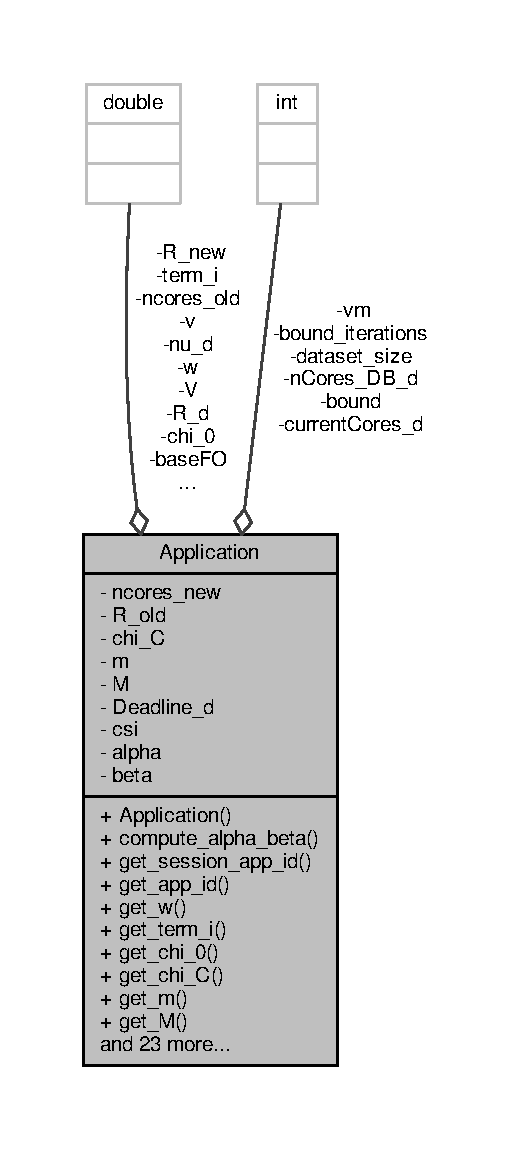
\includegraphics[width=309pt]{classApplication__coll__graph}
\end{center}
\end{figure}
\subsection*{Public Member Functions}
\begin{DoxyCompactItemize}
\item 
\hyperlink{classApplication_aa660e2135b162cfddaca0918be8599e8}{Application} (std\-::string \hyperlink{classApplication_a5e28ffadb86925ecae57ab18c0085d90}{session\-\_\-app\-\_\-id}, std\-::string \hyperlink{classApplication_a05377e6cdcb9d48f29e0f1972a4a16fe}{app\-\_\-id}, double \hyperlink{classApplication_aead1b7b0150c2a3ebd6c36b1db8c4732}{w}, double \hyperlink{classApplication_a3b9dab40d189989c836b8d328946bbb6}{chi\-\_\-0}, double \hyperlink{classApplication_a46e29a6bfc74de610feec809a77dfb62}{chi\-\_\-\-C}, double \hyperlink{classApplication_ab903d83d3cde51569a27f97752c9f158}{m}, double \hyperlink{classApplication_a14904a2abf46cc0a50eb82043fa0912e}{M}, double \hyperlink{classApplication_aa92ad37e6701931176e0dc9b260fd7ee}{V}, double \hyperlink{classApplication_a9efc167094a42382504dd28a7ac402e0}{v}, double D, double \hyperlink{classApplication_a20adc533c6b6147342b3f60dc0fbd9bc}{csi}, std\-::string St, int Dataset\-Size)
\item 
double \hyperlink{classApplication_a97054cee52b315da040098c3927c909e}{Obj\-Function\-Component} (\hyperlink{readConfigurationFile_8hh_ab8f35b1da3261263c5e9c0e7c8921f5c}{s\-Configuration} \&configuration, M\-Y\-S\-Q\-L $\ast$conn, \hyperlink{classoptJrParameters}{opt\-Jr\-Parameters} \&par)
\end{DoxyCompactItemize}
\subsection*{Public Attributes}
\begin{DoxyCompactItemize}
\item 
int \hyperlink{classApplication_abc7e87e8cbe2e64fa4e2ff2afdf7a4fc}{mode}
\item 
std\-::string \hyperlink{classApplication_a5e28ffadb86925ecae57ab18c0085d90}{session\-\_\-app\-\_\-id}
\item 
std\-::string \hyperlink{classApplication_a05377e6cdcb9d48f29e0f1972a4a16fe}{app\-\_\-id}
\item 
double \hyperlink{classApplication_aead1b7b0150c2a3ebd6c36b1db8c4732}{w}
\item 
double \hyperlink{classApplication_ad5486702327ad61e56ed04fb54d58c20}{term\-\_\-i}
\item 
double \hyperlink{classApplication_a3b9dab40d189989c836b8d328946bbb6}{chi\-\_\-0}
\item 
double \hyperlink{classApplication_a46e29a6bfc74de610feec809a77dfb62}{chi\-\_\-\-C}
\item 
double \hyperlink{classApplication_ab903d83d3cde51569a27f97752c9f158}{m}
\item 
double \hyperlink{classApplication_a14904a2abf46cc0a50eb82043fa0912e}{M}
\item 
double \hyperlink{classApplication_aa92ad37e6701931176e0dc9b260fd7ee}{V}
\item 
double \hyperlink{classApplication_a9efc167094a42382504dd28a7ac402e0}{v}
\item 
double \hyperlink{classApplication_a2a989ae288a74ee5250b5acf449c864a}{Deadline\-\_\-d}
\item 
double \hyperlink{classApplication_a20adc533c6b6147342b3f60dc0fbd9bc}{csi}
\item 
std\-::string \hyperlink{classApplication_adb1cba2c06695bfdf81482dfba449d5b}{stage}
\item 
int \hyperlink{classApplication_aaa155e818d807f585d83ecacf4abfe42}{dataset\-Size}
\item 
double \hyperlink{classApplication_a42c22b9a3130cf1f2722ce222f2e5bae}{nu\-\_\-d}
\item 
int \hyperlink{classApplication_adee341a84a5389dfd4d16e7f8e697190}{current\-Cores\-\_\-d}
\item 
int \hyperlink{classApplication_a95104d330c9c7ed2c1017b4938a39a9a}{n\-Cores\-\_\-\-D\-B\-\_\-d}
\item 
int \hyperlink{classApplication_a6e91bef9d503af0e8ba38c8f445c8cb0}{bound}
\item 
double \hyperlink{classApplication_a374d43f68ae27aaed98278e8152a434c}{R\-\_\-d}
\item 
double \hyperlink{classApplication_a32da2e06513ef910601d75eb89bb528b}{R\-\_\-bound\-\_\-d}
\item 
double \hyperlink{classApplication_aa703e7525d446d98b5cd51c959d35998}{base\-F\-O}
\item 
double \hyperlink{classApplication_a95fd54cbed658fb23ce27939666c91d2}{initial\-Base\-F\-O}
\item 
float \hyperlink{classApplication_a087ef34a09792f2954940324dcea20d6}{alpha}
\item 
float \hyperlink{classApplication_a7c74ef816a425a4115005d15d01ac9c6}{beta}
\item 
\hyperlink{classsAlphaBetaManagement}{s\-Alpha\-Beta\-Management} \hyperlink{classApplication_a6bbd698f2df7c4cedb9fb46fce23dbfe}{s\-A\-B}
\item 
int \hyperlink{classApplication_a6a3692743eccba602a58fdfc3f23950b}{bound\-Iterations}
\item 
int \hyperlink{classApplication_a0a3fe386eb8244e536bc5297709d1269}{vm}
\end{DoxyCompactItemize}


\subsection{Constructor \& Destructor Documentation}
\hypertarget{classApplication_aa660e2135b162cfddaca0918be8599e8}{\index{Application@{Application}!Application@{Application}}
\index{Application@{Application}!Application@{Application}}
\subsubsection[{Application}]{\setlength{\rightskip}{0pt plus 5cm}Application\-::\-Application (
\begin{DoxyParamCaption}
\item[{std\-::string}]{session\-\_\-app\-\_\-id, }
\item[{std\-::string}]{app\-\_\-id, }
\item[{double}]{w, }
\item[{double}]{chi\-\_\-0, }
\item[{double}]{chi\-\_\-\-C, }
\item[{double}]{m, }
\item[{double}]{M, }
\item[{double}]{V, }
\item[{double}]{v, }
\item[{double}]{D, }
\item[{double}]{csi, }
\item[{std\-::string}]{St, }
\item[{int}]{Dataset\-Size}
\end{DoxyParamCaption}
)}}\label{classApplication_aa660e2135b162cfddaca0918be8599e8}


\subsection{Member Function Documentation}
\hypertarget{classApplication_a97054cee52b315da040098c3927c909e}{\index{Application@{Application}!Obj\-Function\-Component@{Obj\-Function\-Component}}
\index{Obj\-Function\-Component@{Obj\-Function\-Component}!Application@{Application}}
\subsubsection[{Obj\-Function\-Component}]{\setlength{\rightskip}{0pt plus 5cm}double Application\-::\-Obj\-Function\-Component (
\begin{DoxyParamCaption}
\item[{{\bf s\-Configuration} \&}]{configuration, }
\item[{M\-Y\-S\-Q\-L $\ast$}]{conn, }
\item[{{\bf opt\-Jr\-Parameters} \&}]{par}
\end{DoxyParamCaption}
)}}\label{classApplication_a97054cee52b315da040098c3927c909e}


Here is the call graph for this function\-:\nopagebreak
\begin{figure}[H]
\begin{center}
\leavevmode
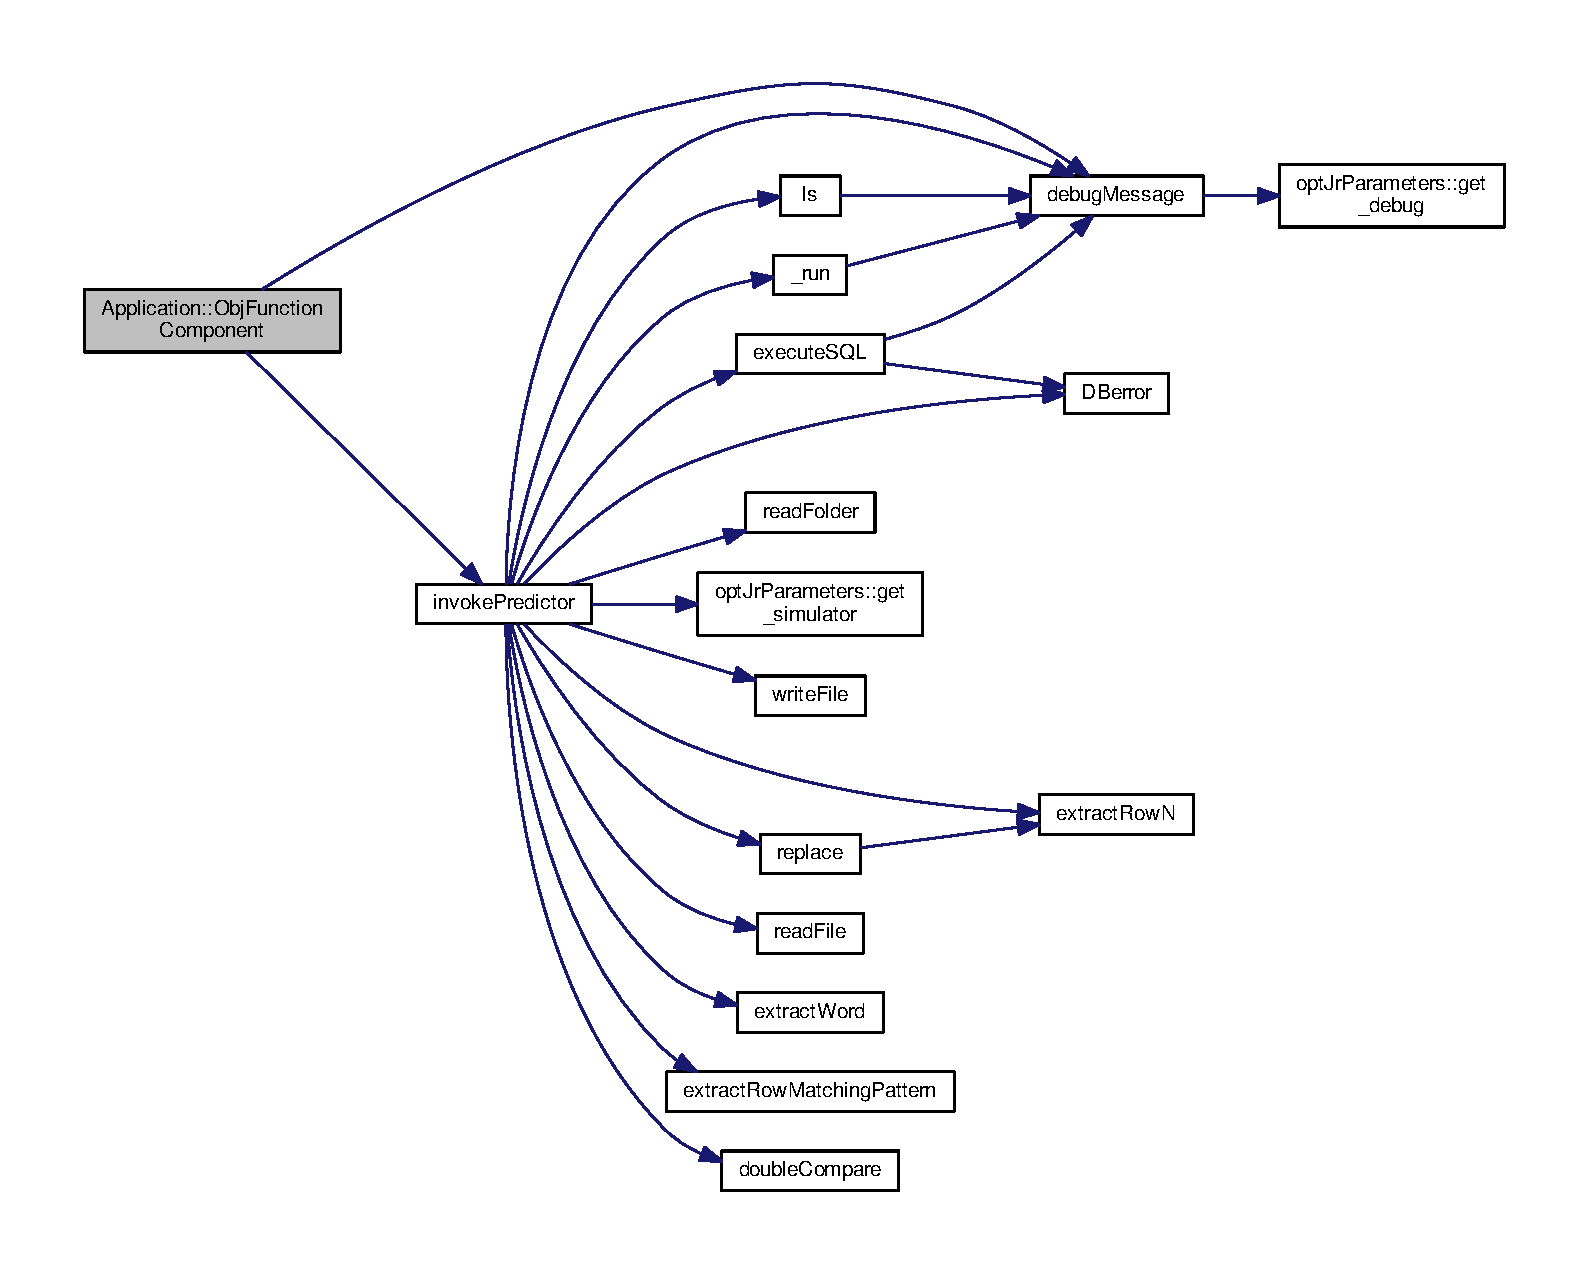
\includegraphics[width=350pt]{classApplication_a97054cee52b315da040098c3927c909e_cgraph}
\end{center}
\end{figure}




\subsection{Member Data Documentation}
\hypertarget{classApplication_a087ef34a09792f2954940324dcea20d6}{\index{Application@{Application}!alpha@{alpha}}
\index{alpha@{alpha}!Application@{Application}}
\subsubsection[{alpha}]{\setlength{\rightskip}{0pt plus 5cm}float Application\-::alpha}}\label{classApplication_a087ef34a09792f2954940324dcea20d6}
\hypertarget{classApplication_a05377e6cdcb9d48f29e0f1972a4a16fe}{\index{Application@{Application}!app\-\_\-id@{app\-\_\-id}}
\index{app\-\_\-id@{app\-\_\-id}!Application@{Application}}
\subsubsection[{app\-\_\-id}]{\setlength{\rightskip}{0pt plus 5cm}std\-::string Application\-::app\-\_\-id}}\label{classApplication_a05377e6cdcb9d48f29e0f1972a4a16fe}
\hypertarget{classApplication_aa703e7525d446d98b5cd51c959d35998}{\index{Application@{Application}!base\-F\-O@{base\-F\-O}}
\index{base\-F\-O@{base\-F\-O}!Application@{Application}}
\subsubsection[{base\-F\-O}]{\setlength{\rightskip}{0pt plus 5cm}double Application\-::base\-F\-O}}\label{classApplication_aa703e7525d446d98b5cd51c959d35998}
\hypertarget{classApplication_a7c74ef816a425a4115005d15d01ac9c6}{\index{Application@{Application}!beta@{beta}}
\index{beta@{beta}!Application@{Application}}
\subsubsection[{beta}]{\setlength{\rightskip}{0pt plus 5cm}float Application\-::beta}}\label{classApplication_a7c74ef816a425a4115005d15d01ac9c6}
\hypertarget{classApplication_a6e91bef9d503af0e8ba38c8f445c8cb0}{\index{Application@{Application}!bound@{bound}}
\index{bound@{bound}!Application@{Application}}
\subsubsection[{bound}]{\setlength{\rightskip}{0pt plus 5cm}int Application\-::bound}}\label{classApplication_a6e91bef9d503af0e8ba38c8f445c8cb0}
\hypertarget{classApplication_a6a3692743eccba602a58fdfc3f23950b}{\index{Application@{Application}!bound\-Iterations@{bound\-Iterations}}
\index{bound\-Iterations@{bound\-Iterations}!Application@{Application}}
\subsubsection[{bound\-Iterations}]{\setlength{\rightskip}{0pt plus 5cm}int Application\-::bound\-Iterations}}\label{classApplication_a6a3692743eccba602a58fdfc3f23950b}
\hypertarget{classApplication_a3b9dab40d189989c836b8d328946bbb6}{\index{Application@{Application}!chi\-\_\-0@{chi\-\_\-0}}
\index{chi\-\_\-0@{chi\-\_\-0}!Application@{Application}}
\subsubsection[{chi\-\_\-0}]{\setlength{\rightskip}{0pt plus 5cm}double Application\-::chi\-\_\-0}}\label{classApplication_a3b9dab40d189989c836b8d328946bbb6}
\hypertarget{classApplication_a46e29a6bfc74de610feec809a77dfb62}{\index{Application@{Application}!chi\-\_\-\-C@{chi\-\_\-\-C}}
\index{chi\-\_\-\-C@{chi\-\_\-\-C}!Application@{Application}}
\subsubsection[{chi\-\_\-\-C}]{\setlength{\rightskip}{0pt plus 5cm}double Application\-::chi\-\_\-\-C}}\label{classApplication_a46e29a6bfc74de610feec809a77dfb62}
\hypertarget{classApplication_a20adc533c6b6147342b3f60dc0fbd9bc}{\index{Application@{Application}!csi@{csi}}
\index{csi@{csi}!Application@{Application}}
\subsubsection[{csi}]{\setlength{\rightskip}{0pt plus 5cm}double Application\-::csi}}\label{classApplication_a20adc533c6b6147342b3f60dc0fbd9bc}
\hypertarget{classApplication_adee341a84a5389dfd4d16e7f8e697190}{\index{Application@{Application}!current\-Cores\-\_\-d@{current\-Cores\-\_\-d}}
\index{current\-Cores\-\_\-d@{current\-Cores\-\_\-d}!Application@{Application}}
\subsubsection[{current\-Cores\-\_\-d}]{\setlength{\rightskip}{0pt plus 5cm}int Application\-::current\-Cores\-\_\-d}}\label{classApplication_adee341a84a5389dfd4d16e7f8e697190}
\hypertarget{classApplication_aaa155e818d807f585d83ecacf4abfe42}{\index{Application@{Application}!dataset\-Size@{dataset\-Size}}
\index{dataset\-Size@{dataset\-Size}!Application@{Application}}
\subsubsection[{dataset\-Size}]{\setlength{\rightskip}{0pt plus 5cm}int Application\-::dataset\-Size}}\label{classApplication_aaa155e818d807f585d83ecacf4abfe42}
\hypertarget{classApplication_a2a989ae288a74ee5250b5acf449c864a}{\index{Application@{Application}!Deadline\-\_\-d@{Deadline\-\_\-d}}
\index{Deadline\-\_\-d@{Deadline\-\_\-d}!Application@{Application}}
\subsubsection[{Deadline\-\_\-d}]{\setlength{\rightskip}{0pt plus 5cm}double Application\-::\-Deadline\-\_\-d}}\label{classApplication_a2a989ae288a74ee5250b5acf449c864a}
\hypertarget{classApplication_a95fd54cbed658fb23ce27939666c91d2}{\index{Application@{Application}!initial\-Base\-F\-O@{initial\-Base\-F\-O}}
\index{initial\-Base\-F\-O@{initial\-Base\-F\-O}!Application@{Application}}
\subsubsection[{initial\-Base\-F\-O}]{\setlength{\rightskip}{0pt plus 5cm}double Application\-::initial\-Base\-F\-O}}\label{classApplication_a95fd54cbed658fb23ce27939666c91d2}
\hypertarget{classApplication_ab903d83d3cde51569a27f97752c9f158}{\index{Application@{Application}!m@{m}}
\index{m@{m}!Application@{Application}}
\subsubsection[{m}]{\setlength{\rightskip}{0pt plus 5cm}double Application\-::m}}\label{classApplication_ab903d83d3cde51569a27f97752c9f158}
\hypertarget{classApplication_a14904a2abf46cc0a50eb82043fa0912e}{\index{Application@{Application}!M@{M}}
\index{M@{M}!Application@{Application}}
\subsubsection[{M}]{\setlength{\rightskip}{0pt plus 5cm}double Application\-::\-M}}\label{classApplication_a14904a2abf46cc0a50eb82043fa0912e}
\hypertarget{classApplication_abc7e87e8cbe2e64fa4e2ff2afdf7a4fc}{\index{Application@{Application}!mode@{mode}}
\index{mode@{mode}!Application@{Application}}
\subsubsection[{mode}]{\setlength{\rightskip}{0pt plus 5cm}int Application\-::mode}}\label{classApplication_abc7e87e8cbe2e64fa4e2ff2afdf7a4fc}
\hypertarget{classApplication_a95104d330c9c7ed2c1017b4938a39a9a}{\index{Application@{Application}!n\-Cores\-\_\-\-D\-B\-\_\-d@{n\-Cores\-\_\-\-D\-B\-\_\-d}}
\index{n\-Cores\-\_\-\-D\-B\-\_\-d@{n\-Cores\-\_\-\-D\-B\-\_\-d}!Application@{Application}}
\subsubsection[{n\-Cores\-\_\-\-D\-B\-\_\-d}]{\setlength{\rightskip}{0pt plus 5cm}int Application\-::n\-Cores\-\_\-\-D\-B\-\_\-d}}\label{classApplication_a95104d330c9c7ed2c1017b4938a39a9a}
\hypertarget{classApplication_a42c22b9a3130cf1f2722ce222f2e5bae}{\index{Application@{Application}!nu\-\_\-d@{nu\-\_\-d}}
\index{nu\-\_\-d@{nu\-\_\-d}!Application@{Application}}
\subsubsection[{nu\-\_\-d}]{\setlength{\rightskip}{0pt plus 5cm}double Application\-::nu\-\_\-d}}\label{classApplication_a42c22b9a3130cf1f2722ce222f2e5bae}
\hypertarget{classApplication_a32da2e06513ef910601d75eb89bb528b}{\index{Application@{Application}!R\-\_\-bound\-\_\-d@{R\-\_\-bound\-\_\-d}}
\index{R\-\_\-bound\-\_\-d@{R\-\_\-bound\-\_\-d}!Application@{Application}}
\subsubsection[{R\-\_\-bound\-\_\-d}]{\setlength{\rightskip}{0pt plus 5cm}double Application\-::\-R\-\_\-bound\-\_\-d}}\label{classApplication_a32da2e06513ef910601d75eb89bb528b}
\hypertarget{classApplication_a374d43f68ae27aaed98278e8152a434c}{\index{Application@{Application}!R\-\_\-d@{R\-\_\-d}}
\index{R\-\_\-d@{R\-\_\-d}!Application@{Application}}
\subsubsection[{R\-\_\-d}]{\setlength{\rightskip}{0pt plus 5cm}double Application\-::\-R\-\_\-d}}\label{classApplication_a374d43f68ae27aaed98278e8152a434c}
\hypertarget{classApplication_a6bbd698f2df7c4cedb9fb46fce23dbfe}{\index{Application@{Application}!s\-A\-B@{s\-A\-B}}
\index{s\-A\-B@{s\-A\-B}!Application@{Application}}
\subsubsection[{s\-A\-B}]{\setlength{\rightskip}{0pt plus 5cm}{\bf s\-Alpha\-Beta\-Management} Application\-::s\-A\-B}}\label{classApplication_a6bbd698f2df7c4cedb9fb46fce23dbfe}
\hypertarget{classApplication_a5e28ffadb86925ecae57ab18c0085d90}{\index{Application@{Application}!session\-\_\-app\-\_\-id@{session\-\_\-app\-\_\-id}}
\index{session\-\_\-app\-\_\-id@{session\-\_\-app\-\_\-id}!Application@{Application}}
\subsubsection[{session\-\_\-app\-\_\-id}]{\setlength{\rightskip}{0pt plus 5cm}std\-::string Application\-::session\-\_\-app\-\_\-id}}\label{classApplication_a5e28ffadb86925ecae57ab18c0085d90}
\hypertarget{classApplication_adb1cba2c06695bfdf81482dfba449d5b}{\index{Application@{Application}!stage@{stage}}
\index{stage@{stage}!Application@{Application}}
\subsubsection[{stage}]{\setlength{\rightskip}{0pt plus 5cm}std\-::string Application\-::stage}}\label{classApplication_adb1cba2c06695bfdf81482dfba449d5b}
\hypertarget{classApplication_ad5486702327ad61e56ed04fb54d58c20}{\index{Application@{Application}!term\-\_\-i@{term\-\_\-i}}
\index{term\-\_\-i@{term\-\_\-i}!Application@{Application}}
\subsubsection[{term\-\_\-i}]{\setlength{\rightskip}{0pt plus 5cm}double Application\-::term\-\_\-i}}\label{classApplication_ad5486702327ad61e56ed04fb54d58c20}
\hypertarget{classApplication_aa92ad37e6701931176e0dc9b260fd7ee}{\index{Application@{Application}!V@{V}}
\index{V@{V}!Application@{Application}}
\subsubsection[{V}]{\setlength{\rightskip}{0pt plus 5cm}double Application\-::\-V}}\label{classApplication_aa92ad37e6701931176e0dc9b260fd7ee}
\hypertarget{classApplication_a9efc167094a42382504dd28a7ac402e0}{\index{Application@{Application}!v@{v}}
\index{v@{v}!Application@{Application}}
\subsubsection[{v}]{\setlength{\rightskip}{0pt plus 5cm}double Application\-::v}}\label{classApplication_a9efc167094a42382504dd28a7ac402e0}
\hypertarget{classApplication_a0a3fe386eb8244e536bc5297709d1269}{\index{Application@{Application}!vm@{vm}}
\index{vm@{vm}!Application@{Application}}
\subsubsection[{vm}]{\setlength{\rightskip}{0pt plus 5cm}int Application\-::vm}}\label{classApplication_a0a3fe386eb8244e536bc5297709d1269}
\hypertarget{classApplication_aead1b7b0150c2a3ebd6c36b1db8c4732}{\index{Application@{Application}!w@{w}}
\index{w@{w}!Application@{Application}}
\subsubsection[{w}]{\setlength{\rightskip}{0pt plus 5cm}double Application\-::w}}\label{classApplication_aead1b7b0150c2a3ebd6c36b1db8c4732}


The documentation for this class was generated from the following files\-:\begin{DoxyCompactItemize}
\item 
/vagrant/\-P\-R\-O\-J\-E\-C\-T\-\_\-\-S\-P\-A\-R\-K/\-P\-A\-C\-S\-\_\-\-P\-R\-O\-J\-E\-C\-T/opt\-\_\-jr/src/\hyperlink{application_8hh}{application.\-hh}\item 
/vagrant/\-P\-R\-O\-J\-E\-C\-T\-\_\-\-S\-P\-A\-R\-K/\-P\-A\-C\-S\-\_\-\-P\-R\-O\-J\-E\-C\-T/opt\-\_\-jr/src/\hyperlink{application_8cpp}{application.\-cpp}\end{DoxyCompactItemize}

\hypertarget{classBatch}{\section{Batch Class Reference}
\label{classBatch}\index{Batch@{Batch}}
}


{\ttfamily \#include $<$batch.\-hh$>$}



Collaboration diagram for Batch\-:\nopagebreak
\begin{figure}[H]
\begin{center}
\leavevmode
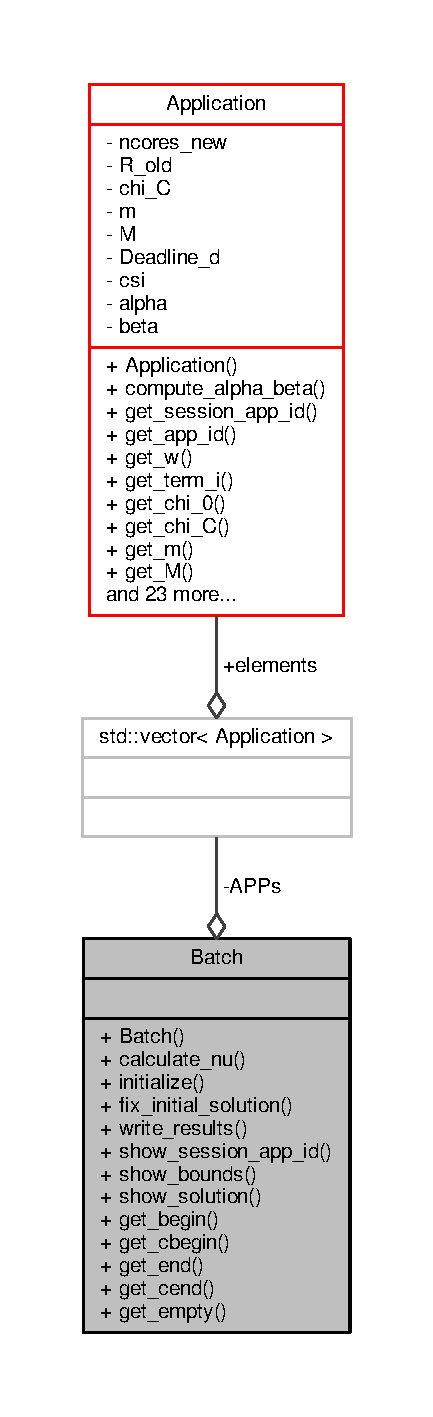
\includegraphics[width=309pt]{classBatch__coll__graph}
\end{center}
\end{figure}
\subsection*{Public Member Functions}
\begin{DoxyCompactItemize}
\item 
\hyperlink{classBatch_aea459d16c99c2f02af53b3ad5b0ff12d}{Batch} (std\-::vector$<$ \hyperlink{classApplication}{Application} $>$ apps)
\item 
void \hyperlink{classBatch_a14f132321413b45d6446200807451414}{calculate\-\_\-nu} (\hyperlink{classoptJrParameters}{opt\-Jr\-Parameters} \&par)
\item 
void \hyperlink{classBatch_ae212d22fa812b51160f57507242152c1}{initialize} (\hyperlink{readConfigurationFile_8hh_ab8f35b1da3261263c5e9c0e7c8921f5c}{s\-Configuration} \&configuration, M\-Y\-S\-Q\-L $\ast$conn, \hyperlink{classoptJrParameters}{opt\-Jr\-Parameters} \&par)
\item 
void \hyperlink{classBatch_ac50dad870490ca7c60e0e15d86c02614}{fix\-Initial\-Solution} (\hyperlink{classoptJrParameters}{opt\-Jr\-Parameters} \&par)
\item 
\hyperlink{candidates_8hh_af1ec7d668b0f7361dc7e1e1da5c4ce7d}{s\-Candidates} \hyperlink{classBatch_acf54e153a40b4720b1f7bebf000b1600}{approximated\-Loop} (int \&iteration, \hyperlink{classoptJrParameters}{opt\-Jr\-Parameters} \&par)
\end{DoxyCompactItemize}
\subsection*{Public Attributes}
\begin{DoxyCompactItemize}
\item 
std\-::vector$<$ \hyperlink{classApplication}{Application} $>$ \hyperlink{classBatch_a757bf1a36fee46b1b47263ab4a59c560}{A\-P\-Ps}
\end{DoxyCompactItemize}


\subsection{Constructor \& Destructor Documentation}
\hypertarget{classBatch_aea459d16c99c2f02af53b3ad5b0ff12d}{\index{Batch@{Batch}!Batch@{Batch}}
\index{Batch@{Batch}!Batch@{Batch}}
\subsubsection[{Batch}]{\setlength{\rightskip}{0pt plus 5cm}Batch\-::\-Batch (
\begin{DoxyParamCaption}
\item[{std\-::vector$<$ {\bf Application} $>$}]{apps}
\end{DoxyParamCaption}
)\hspace{0.3cm}{\ttfamily [inline]}}}\label{classBatch_aea459d16c99c2f02af53b3ad5b0ff12d}


\subsection{Member Function Documentation}
\hypertarget{classBatch_acf54e153a40b4720b1f7bebf000b1600}{\index{Batch@{Batch}!approximated\-Loop@{approximated\-Loop}}
\index{approximated\-Loop@{approximated\-Loop}!Batch@{Batch}}
\subsubsection[{approximated\-Loop}]{\setlength{\rightskip}{0pt plus 5cm}{\bf s\-Candidates} Batch\-::approximated\-Loop (
\begin{DoxyParamCaption}
\item[{int \&}]{iteration, }
\item[{{\bf opt\-Jr\-Parameters} \&}]{par}
\end{DoxyParamCaption}
)}}\label{classBatch_acf54e153a40b4720b1f7bebf000b1600}


Here is the call graph for this function\-:\nopagebreak
\begin{figure}[H]
\begin{center}
\leavevmode
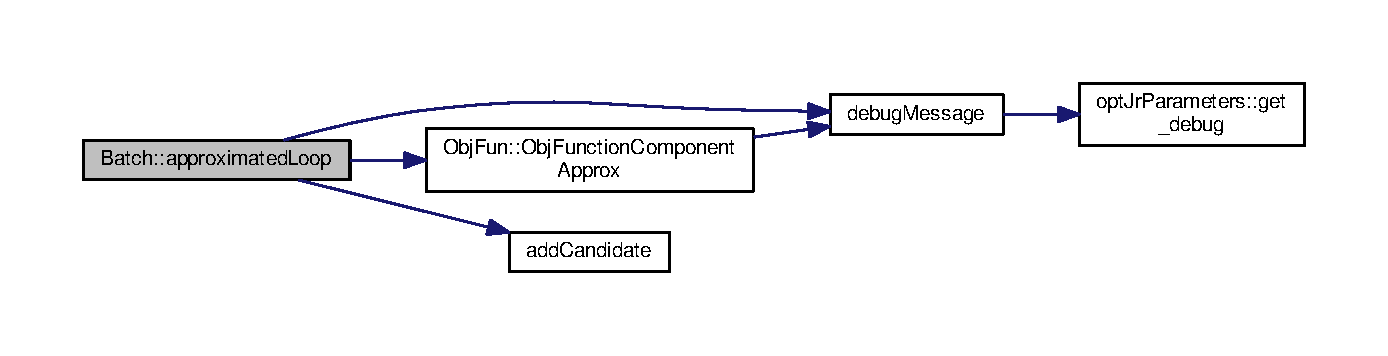
\includegraphics[width=350pt]{classBatch_acf54e153a40b4720b1f7bebf000b1600_cgraph}
\end{center}
\end{figure}




Here is the caller graph for this function\-:\nopagebreak
\begin{figure}[H]
\begin{center}
\leavevmode
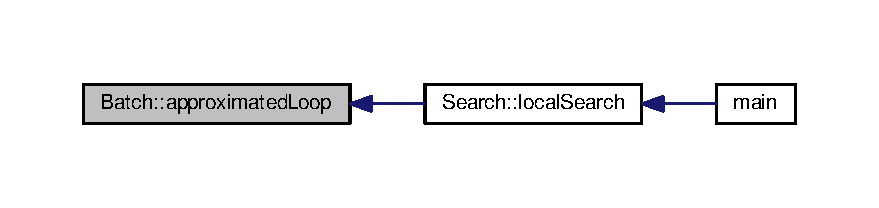
\includegraphics[width=350pt]{classBatch_acf54e153a40b4720b1f7bebf000b1600_icgraph}
\end{center}
\end{figure}


\hypertarget{classBatch_a14f132321413b45d6446200807451414}{\index{Batch@{Batch}!calculate\-\_\-nu@{calculate\-\_\-nu}}
\index{calculate\-\_\-nu@{calculate\-\_\-nu}!Batch@{Batch}}
\subsubsection[{calculate\-\_\-nu}]{\setlength{\rightskip}{0pt plus 5cm}void Batch\-::calculate\-\_\-nu (
\begin{DoxyParamCaption}
\item[{{\bf opt\-Jr\-Parameters} \&}]{par}
\end{DoxyParamCaption}
)}}\label{classBatch_a14f132321413b45d6446200807451414}


Here is the call graph for this function\-:\nopagebreak
\begin{figure}[H]
\begin{center}
\leavevmode
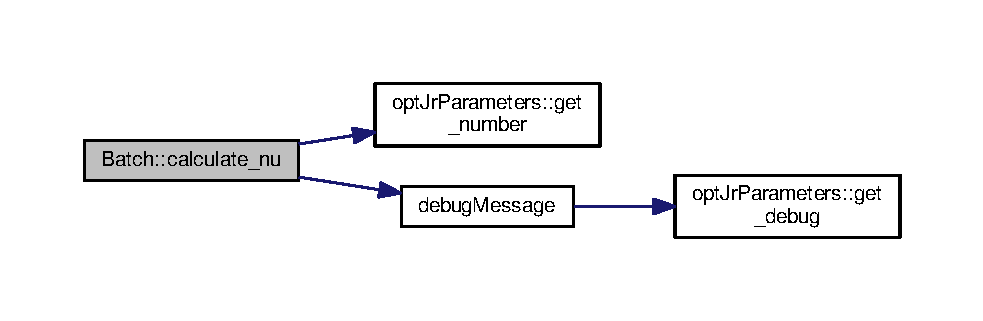
\includegraphics[width=350pt]{classBatch_a14f132321413b45d6446200807451414_cgraph}
\end{center}
\end{figure}




Here is the caller graph for this function\-:\nopagebreak
\begin{figure}[H]
\begin{center}
\leavevmode
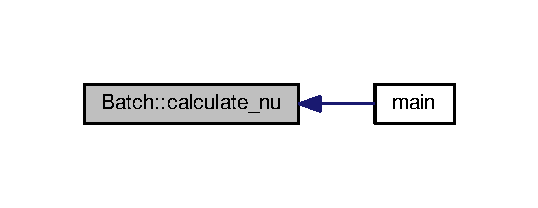
\includegraphics[width=258pt]{classBatch_a14f132321413b45d6446200807451414_icgraph}
\end{center}
\end{figure}


\hypertarget{classBatch_ac50dad870490ca7c60e0e15d86c02614}{\index{Batch@{Batch}!fix\-Initial\-Solution@{fix\-Initial\-Solution}}
\index{fix\-Initial\-Solution@{fix\-Initial\-Solution}!Batch@{Batch}}
\subsubsection[{fix\-Initial\-Solution}]{\setlength{\rightskip}{0pt plus 5cm}void Batch\-::fix\-Initial\-Solution (
\begin{DoxyParamCaption}
\item[{{\bf opt\-Jr\-Parameters} \&}]{par}
\end{DoxyParamCaption}
)}}\label{classBatch_ac50dad870490ca7c60e0e15d86c02614}


Here is the call graph for this function\-:\nopagebreak
\begin{figure}[H]
\begin{center}
\leavevmode
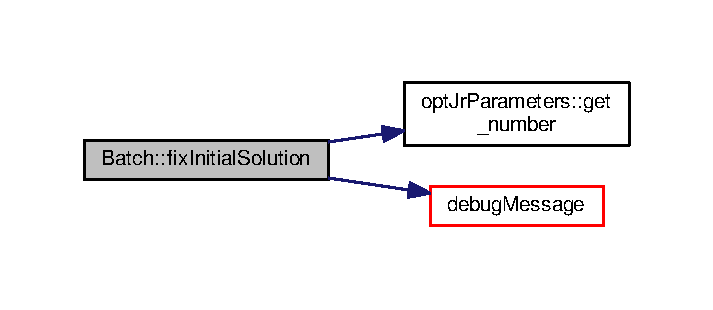
\includegraphics[width=350pt]{classBatch_ac50dad870490ca7c60e0e15d86c02614_cgraph}
\end{center}
\end{figure}




Here is the caller graph for this function\-:\nopagebreak
\begin{figure}[H]
\begin{center}
\leavevmode
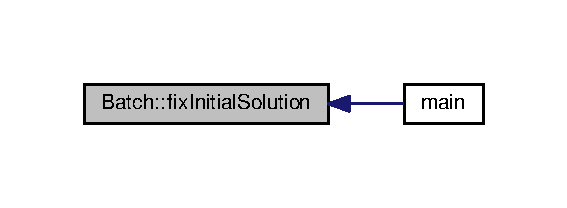
\includegraphics[width=272pt]{classBatch_ac50dad870490ca7c60e0e15d86c02614_icgraph}
\end{center}
\end{figure}


\hypertarget{classBatch_ae212d22fa812b51160f57507242152c1}{\index{Batch@{Batch}!initialize@{initialize}}
\index{initialize@{initialize}!Batch@{Batch}}
\subsubsection[{initialize}]{\setlength{\rightskip}{0pt plus 5cm}void Batch\-::initialize (
\begin{DoxyParamCaption}
\item[{{\bf s\-Configuration} \&}]{configuration, }
\item[{M\-Y\-S\-Q\-L $\ast$}]{conn, }
\item[{{\bf opt\-Jr\-Parameters} \&}]{par}
\end{DoxyParamCaption}
)}}\label{classBatch_ae212d22fa812b51160f57507242152c1}


Here is the call graph for this function\-:\nopagebreak
\begin{figure}[H]
\begin{center}
\leavevmode
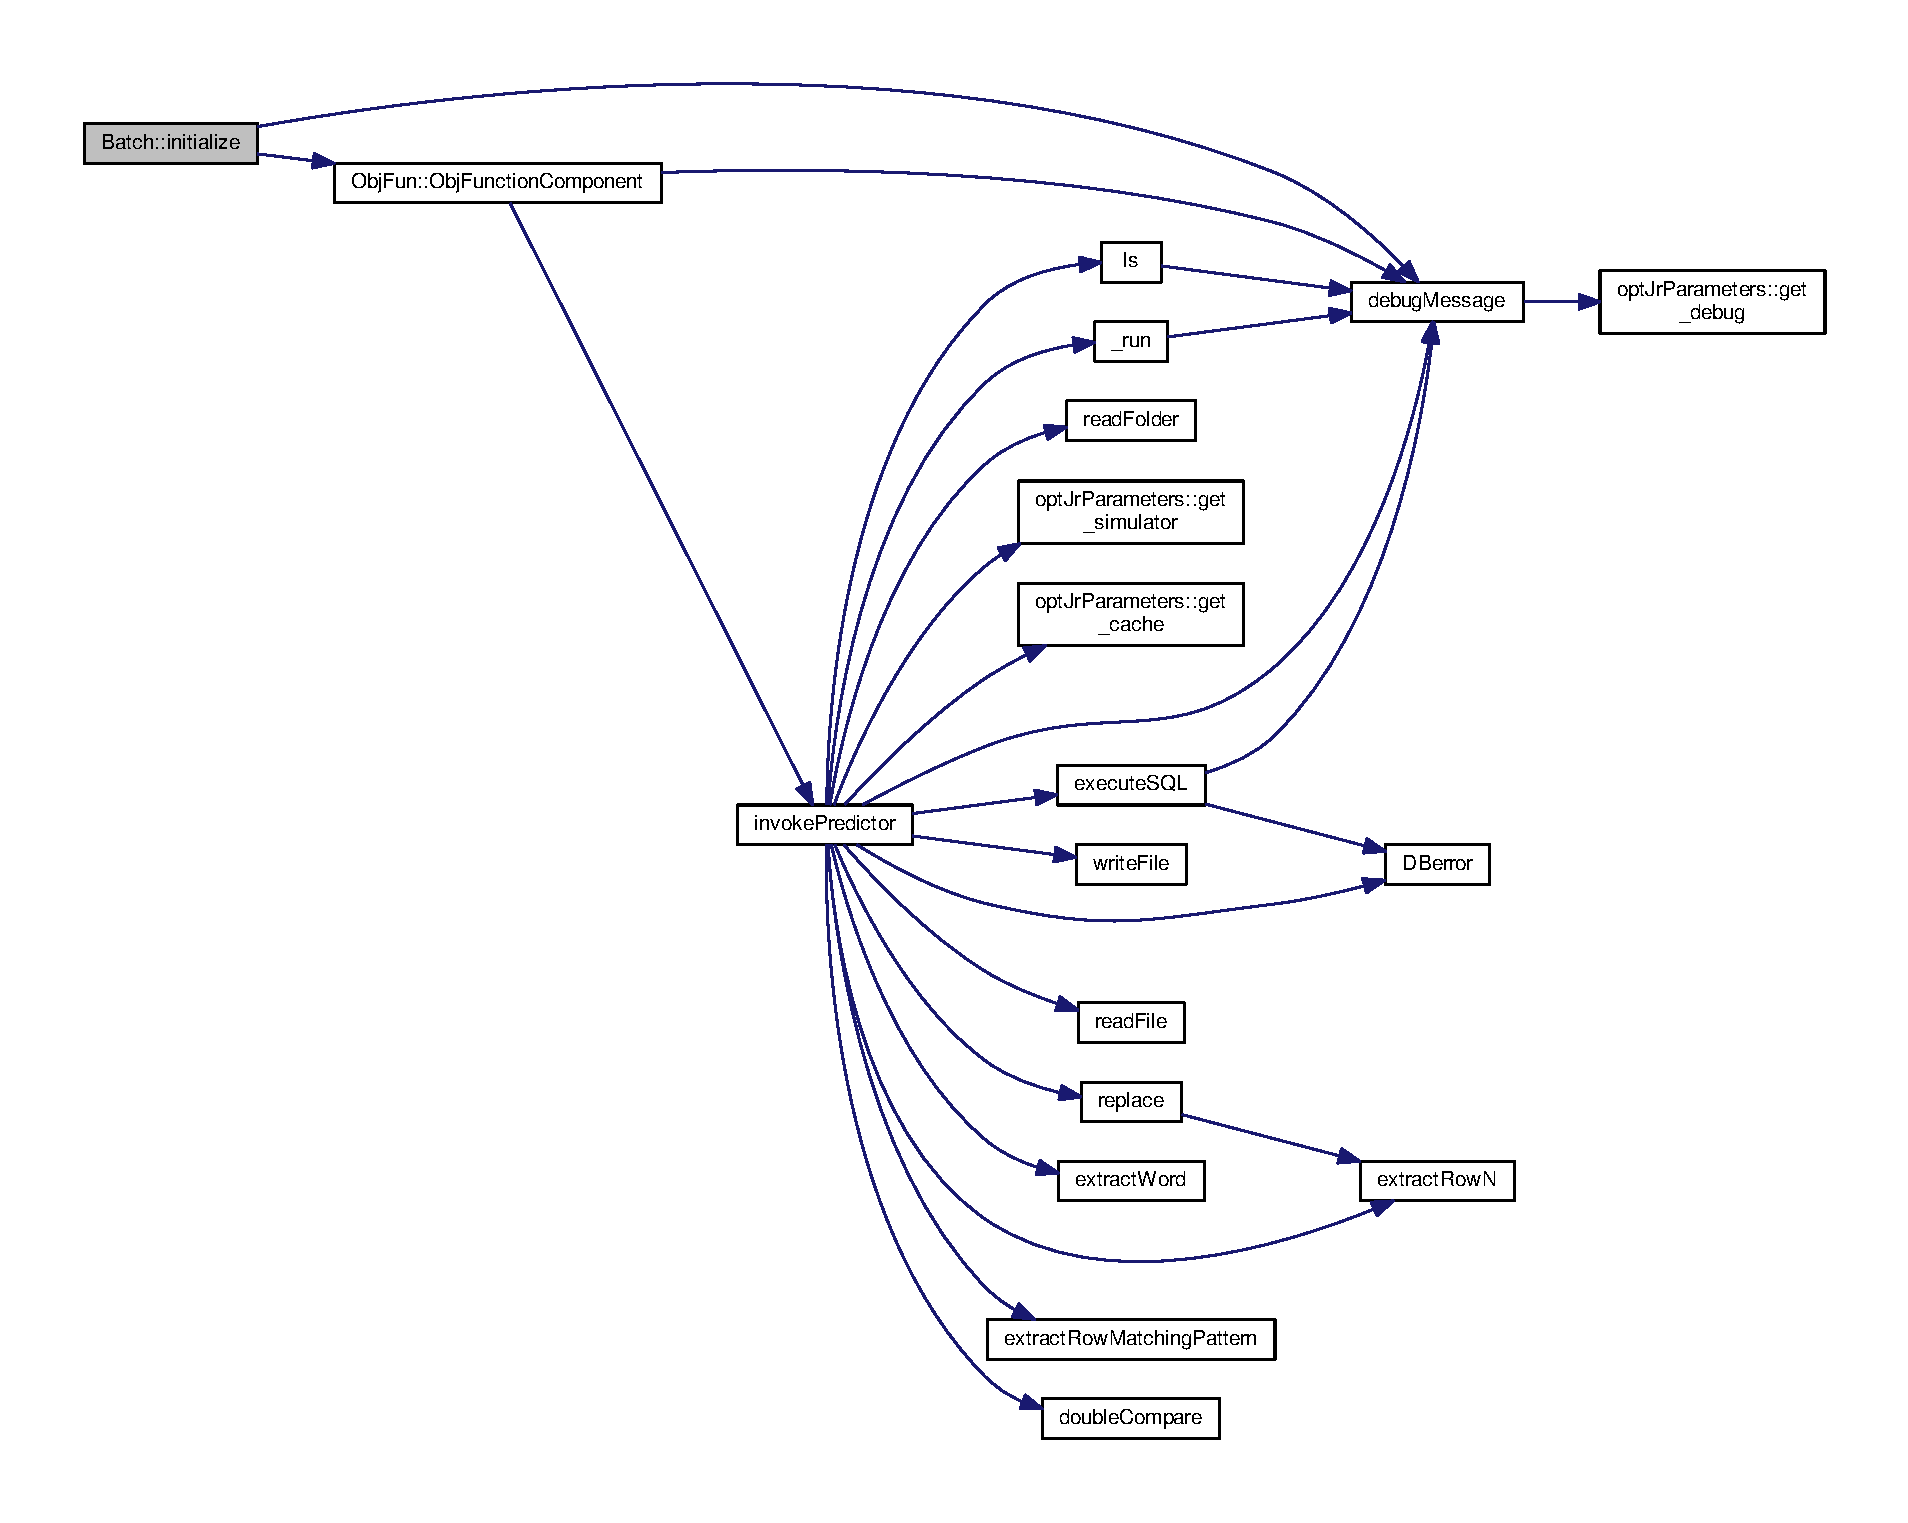
\includegraphics[width=350pt]{classBatch_ae212d22fa812b51160f57507242152c1_cgraph}
\end{center}
\end{figure}




Here is the caller graph for this function\-:\nopagebreak
\begin{figure}[H]
\begin{center}
\leavevmode
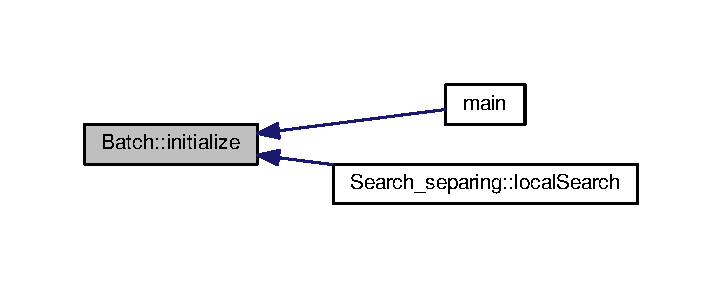
\includegraphics[width=238pt]{classBatch_ae212d22fa812b51160f57507242152c1_icgraph}
\end{center}
\end{figure}




\subsection{Member Data Documentation}
\hypertarget{classBatch_a757bf1a36fee46b1b47263ab4a59c560}{\index{Batch@{Batch}!A\-P\-Ps@{A\-P\-Ps}}
\index{A\-P\-Ps@{A\-P\-Ps}!Batch@{Batch}}
\subsubsection[{A\-P\-Ps}]{\setlength{\rightskip}{0pt plus 5cm}std\-::vector$<${\bf Application}$>$ Batch\-::\-A\-P\-Ps}}\label{classBatch_a757bf1a36fee46b1b47263ab4a59c560}


The documentation for this class was generated from the following files\-:\begin{DoxyCompactItemize}
\item 
/vagrant/\-P\-R\-O\-J\-E\-C\-T\-\_\-\-S\-P\-A\-R\-K/\-P\-A\-C\-S\-\_\-\-P\-R\-O\-J\-E\-C\-T/opt\-\_\-jr/src/\hyperlink{batch_8hh}{batch.\-hh}\item 
/vagrant/\-P\-R\-O\-J\-E\-C\-T\-\_\-\-S\-P\-A\-R\-K/\-P\-A\-C\-S\-\_\-\-P\-R\-O\-J\-E\-C\-T/opt\-\_\-jr/src/\hyperlink{batch_8cpp}{batch.\-cpp}\end{DoxyCompactItemize}

\hypertarget{classBounds}{\section{Bounds Class Reference}
\label{classBounds}\index{Bounds@{Bounds}}
}


{\ttfamily \#include $<$bounds.\-hh$>$}



Collaboration diagram for Bounds\-:
\nopagebreak
\begin{figure}[H]
\begin{center}
\leavevmode
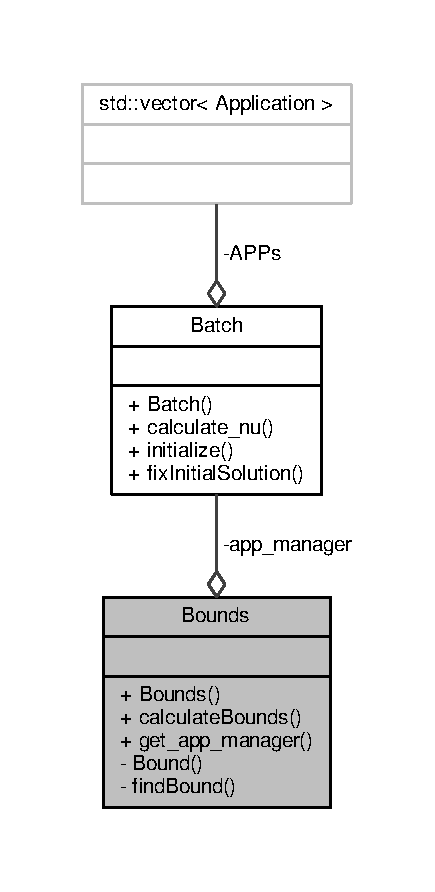
\includegraphics[width=209pt]{classBounds__coll__graph}
\end{center}
\end{figure}
\subsection*{Public Member Functions}
\begin{DoxyCompactItemize}
\item 
\hyperlink{classBounds_a57a9894ee450eb885a83e884b5fb79e7}{Bounds} (\hyperlink{classBatch}{Batch} app\-\_\-m)
\item 
void \hyperlink{classBounds_aefc7e0bd2cd1c5850a903aabe0351dbe}{calculate\-Bounds} (\hyperlink{readConfigurationFile_8hh_ab8f35b1da3261263c5e9c0e7c8921f5c}{s\-Configuration} \&configuration, M\-Y\-S\-Q\-L $\ast$conn, \hyperlink{classoptJrParameters}{opt\-Jr\-Parameters} \&par)
\item 
\hyperlink{classBatch}{Batch} \hyperlink{classBounds_aefebbfe17ca3a7d6a0f6cbf4a0bf2782}{get\-\_\-app\-\_\-manager} ()
\end{DoxyCompactItemize}
\subsection*{Private Member Functions}
\begin{DoxyCompactItemize}
\item 
void \hyperlink{classBounds_a6bc038892059a8181984daff0003065f}{Bound} (\hyperlink{readConfigurationFile_8hh_ab8f35b1da3261263c5e9c0e7c8921f5c}{s\-Configuration} \&configuration, M\-Y\-S\-Q\-L $\ast$conn, \hyperlink{classApplication}{Application} \&app, \hyperlink{classoptJrParameters}{opt\-Jr\-Parameters} \&par, int flag\-Dagsim)
\item 
void \hyperlink{classBounds_ade8356aa22e675868ba98226e4216cf3}{find\-Bound} (\hyperlink{readConfigurationFile_8hh_ab8f35b1da3261263c5e9c0e7c8921f5c}{s\-Configuration} \&configuration, M\-Y\-S\-Q\-L $\ast$conn, char $\ast$db, \hyperlink{classApplication}{Application} \&app, \hyperlink{classoptJrParameters}{opt\-Jr\-Parameters} \&par)
\end{DoxyCompactItemize}
\subsection*{Private Attributes}
\begin{DoxyCompactItemize}
\item 
\hyperlink{classBatch}{Batch} \hyperlink{classBounds_a9b463c00e877b6bf67d9e1ff4f36950b}{app\-\_\-manager}
\end{DoxyCompactItemize}


\subsection{Detailed Description}
\hyperlink{classBounds}{Bounds} class provide a method to evaluate the bound for the applications in B\-A\-T\-C\-H i.\-e. the minimal number of cores necessary to finish the execution before the deadline 

\subsection{Constructor \& Destructor Documentation}
\hypertarget{classBounds_a57a9894ee450eb885a83e884b5fb79e7}{\index{Bounds@{Bounds}!Bounds@{Bounds}}
\index{Bounds@{Bounds}!Bounds@{Bounds}}
\subsubsection[{Bounds}]{\setlength{\rightskip}{0pt plus 5cm}Bounds\-::\-Bounds (
\begin{DoxyParamCaption}
\item[{{\bf Batch}}]{app\-\_\-m}
\end{DoxyParamCaption}
)\hspace{0.3cm}{\ttfamily [inline]}}}\label{classBounds_a57a9894ee450eb885a83e884b5fb79e7}


\subsection{Member Function Documentation}
\hypertarget{classBounds_a6bc038892059a8181984daff0003065f}{\index{Bounds@{Bounds}!Bound@{Bound}}
\index{Bound@{Bound}!Bounds@{Bounds}}
\subsubsection[{Bound}]{\setlength{\rightskip}{0pt plus 5cm}void Bounds\-::\-Bound (
\begin{DoxyParamCaption}
\item[{{\bf s\-Configuration} \&}]{configuration, }
\item[{M\-Y\-S\-Q\-L $\ast$}]{conn, }
\item[{{\bf Application} \&}]{app, }
\item[{{\bf opt\-Jr\-Parameters} \&}]{par, }
\item[{int}]{flag\-Dagsim}
\end{DoxyParamCaption}
)\hspace{0.3cm}{\ttfamily [private]}}}\label{classBounds_a6bc038892059a8181984daff0003065f}


Here is the caller graph for this function\-:\nopagebreak
\begin{figure}[H]
\begin{center}
\leavevmode
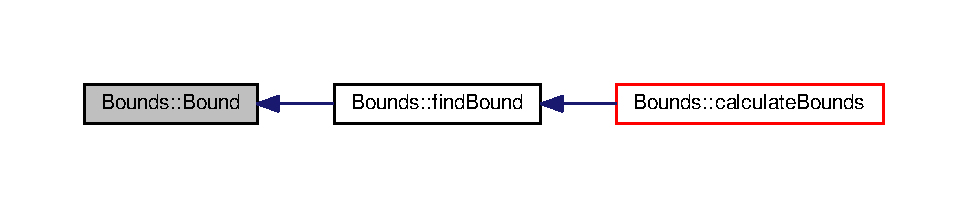
\includegraphics[width=350pt]{classBounds_a6bc038892059a8181984daff0003065f_icgraph}
\end{center}
\end{figure}


\hypertarget{classBounds_aefc7e0bd2cd1c5850a903aabe0351dbe}{\index{Bounds@{Bounds}!calculate\-Bounds@{calculate\-Bounds}}
\index{calculate\-Bounds@{calculate\-Bounds}!Bounds@{Bounds}}
\subsubsection[{calculate\-Bounds}]{\setlength{\rightskip}{0pt plus 5cm}void Bounds\-::calculate\-Bounds (
\begin{DoxyParamCaption}
\item[{{\bf s\-Configuration} \&}]{configuration, }
\item[{M\-Y\-S\-Q\-L $\ast$}]{conn, }
\item[{{\bf opt\-Jr\-Parameters} \&}]{par}
\end{DoxyParamCaption}
)}}\label{classBounds_aefc7e0bd2cd1c5850a903aabe0351dbe}
calculate\-Bounds evaluates the bound for the applications in B\-A\-T\-C\-H i.\-e. the minimal number of cores necessary to finish the execution before the deadline. The function looks before if the result is already stored in the database, otherwise it invokes the predictor doing a \char`\"{}\-H\-I\-L\-L C\-L\-I\-M\-B\-I\-N\-G\char`\"{}. If the number of threads in the configuration file is greater than 0, it does the computations in parallel (using open\-M\-P). 

Here is the caller graph for this function\-:\nopagebreak
\begin{figure}[H]
\begin{center}
\leavevmode
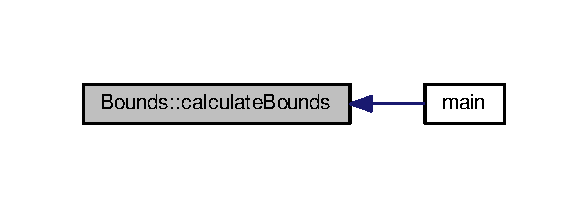
\includegraphics[width=282pt]{classBounds_aefc7e0bd2cd1c5850a903aabe0351dbe_icgraph}
\end{center}
\end{figure}


\hypertarget{classBounds_ade8356aa22e675868ba98226e4216cf3}{\index{Bounds@{Bounds}!find\-Bound@{find\-Bound}}
\index{find\-Bound@{find\-Bound}!Bounds@{Bounds}}
\subsubsection[{find\-Bound}]{\setlength{\rightskip}{0pt plus 5cm}void Bounds\-::find\-Bound (
\begin{DoxyParamCaption}
\item[{{\bf s\-Configuration} \&}]{configuration, }
\item[{M\-Y\-S\-Q\-L $\ast$}]{conn, }
\item[{char $\ast$}]{db, }
\item[{{\bf Application} \&}]{app, }
\item[{{\bf opt\-Jr\-Parameters} \&}]{par}
\end{DoxyParamCaption}
)\hspace{0.3cm}{\ttfamily [private]}}}\label{classBounds_ade8356aa22e675868ba98226e4216cf3}


Here is the caller graph for this function\-:\nopagebreak
\begin{figure}[H]
\begin{center}
\leavevmode
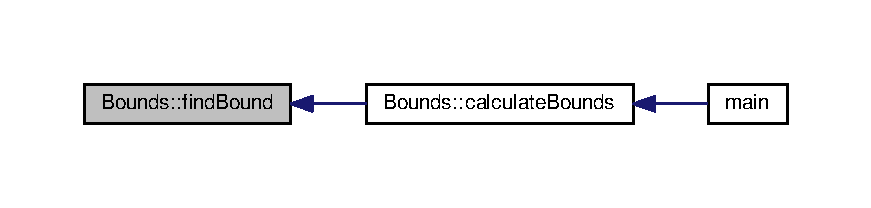
\includegraphics[width=350pt]{classBounds_ade8356aa22e675868ba98226e4216cf3_icgraph}
\end{center}
\end{figure}


\hypertarget{classBounds_aefebbfe17ca3a7d6a0f6cbf4a0bf2782}{\index{Bounds@{Bounds}!get\-\_\-app\-\_\-manager@{get\-\_\-app\-\_\-manager}}
\index{get\-\_\-app\-\_\-manager@{get\-\_\-app\-\_\-manager}!Bounds@{Bounds}}
\subsubsection[{get\-\_\-app\-\_\-manager}]{\setlength{\rightskip}{0pt plus 5cm}{\bf Batch} Bounds\-::get\-\_\-app\-\_\-manager (
\begin{DoxyParamCaption}
{}
\end{DoxyParamCaption}
)\hspace{0.3cm}{\ttfamily [inline]}}}\label{classBounds_aefebbfe17ca3a7d6a0f6cbf4a0bf2782}


Here is the caller graph for this function\-:\nopagebreak
\begin{figure}[H]
\begin{center}
\leavevmode
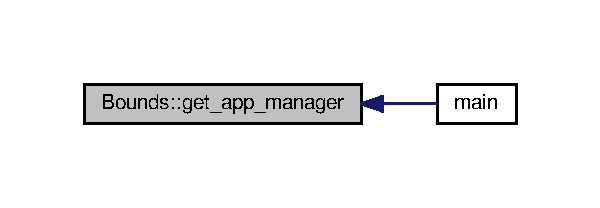
\includegraphics[width=288pt]{classBounds_aefebbfe17ca3a7d6a0f6cbf4a0bf2782_icgraph}
\end{center}
\end{figure}




\subsection{Member Data Documentation}
\hypertarget{classBounds_a9b463c00e877b6bf67d9e1ff4f36950b}{\index{Bounds@{Bounds}!app\-\_\-manager@{app\-\_\-manager}}
\index{app\-\_\-manager@{app\-\_\-manager}!Bounds@{Bounds}}
\subsubsection[{app\-\_\-manager}]{\setlength{\rightskip}{0pt plus 5cm}{\bf Batch} Bounds\-::app\-\_\-manager\hspace{0.3cm}{\ttfamily [private]}}}\label{classBounds_a9b463c00e877b6bf67d9e1ff4f36950b}


The documentation for this class was generated from the following files\-:\begin{DoxyCompactItemize}
\item 
/vagrant/\-P\-R\-O\-J\-E\-C\-T\-\_\-\-S\-P\-A\-R\-K/\-P\-A\-C\-S\-\_\-\-P\-R\-O\-J\-E\-C\-T/opt\-\_\-jr/src/\hyperlink{bounds_8hh}{bounds.\-hh}\item 
/vagrant/\-P\-R\-O\-J\-E\-C\-T\-\_\-\-S\-P\-A\-R\-K/\-P\-A\-C\-S\-\_\-\-P\-R\-O\-J\-E\-C\-T/opt\-\_\-jr/src/\hyperlink{bounds_8cpp}{bounds.\-cpp}\end{DoxyCompactItemize}

\hypertarget{classCandidate__pair}{\section{Candidate\-\_\-pair Class Reference}
\label{classCandidate__pair}\index{Candidate\-\_\-pair@{Candidate\-\_\-pair}}
}


{\ttfamily \#include $<$candidate\-\_\-pair.\-hh$>$}



Collaboration diagram for Candidate\-\_\-pair\-:
\nopagebreak
\begin{figure}[H]
\begin{center}
\leavevmode
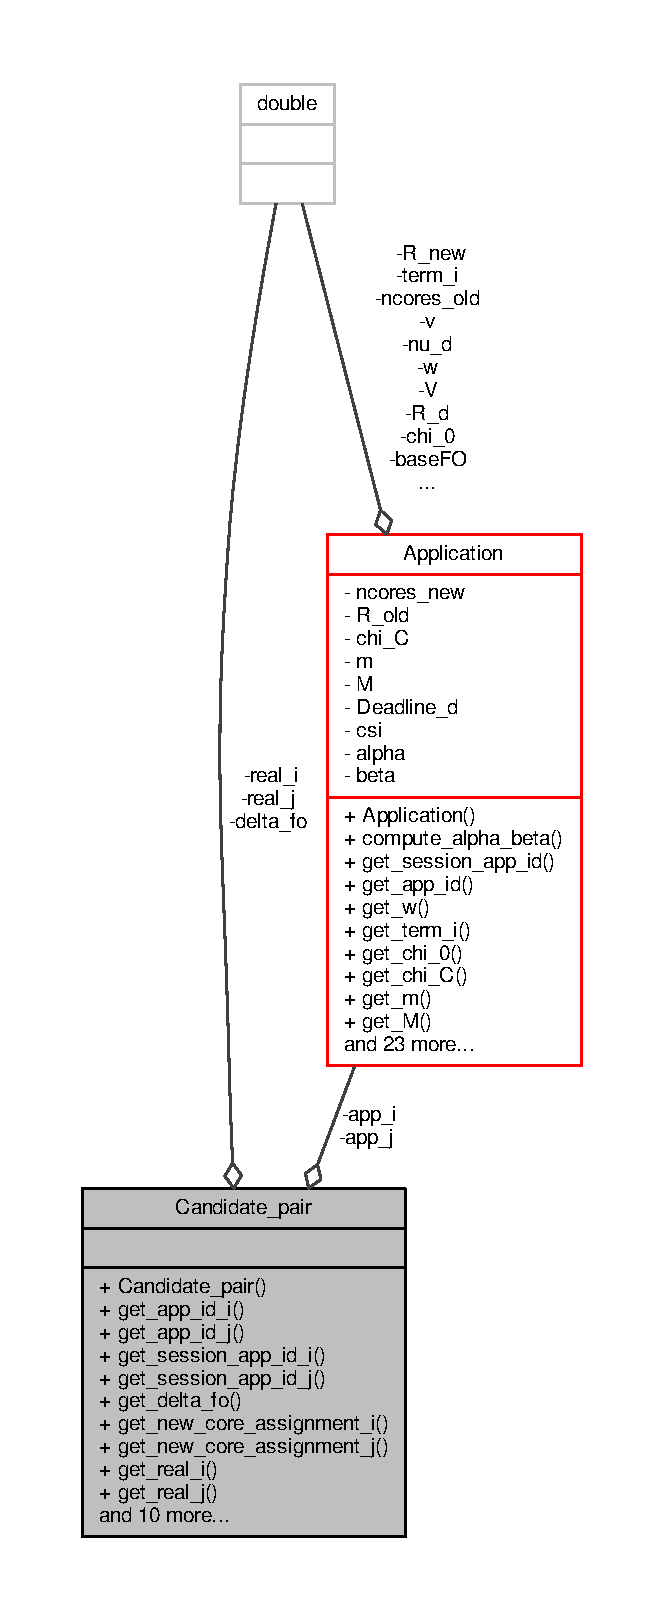
\includegraphics[height=550pt]{classCandidate__pair__coll__graph}
\end{center}
\end{figure}
\subsection*{Public Member Functions}
\begin{DoxyCompactItemize}
\item 
\hyperlink{classCandidate__pair_a59168f369264a7cd8bd7ddb16f23c785}{Candidate\-\_\-pair} (\hyperlink{classApplication}{Application} i, \hyperlink{classApplication}{Application} j, int N\-Ci, int N\-Cj, double D\-\_\-\-F\-O, int d\-\_\-i, int d\-\_\-j)
\begin{DoxyCompactList}\small\item\em Constructor. \end{DoxyCompactList}\item 
const std\-::string \hyperlink{classCandidate__pair_a8fcc74d1e2ad95ab0ecb483a2ceb39b0}{get\-\_\-app\-\_\-id\-\_\-i} ()
\item 
const std\-::string \hyperlink{classCandidate__pair_aaee11e17681cfe95daed61e23b3bd6dc}{get\-\_\-app\-\_\-id\-\_\-j} ()
\item 
const std\-::string \hyperlink{classCandidate__pair_a3d7cb54ffabff340b583925427424085}{get\-\_\-session\-\_\-app\-\_\-id\-\_\-i} ()
\item 
const std\-::string \hyperlink{classCandidate__pair_a8e2faa0c4a09de7667d760a7de0b9596}{get\-\_\-session\-\_\-app\-\_\-id\-\_\-j} ()
\item 
const double \hyperlink{classCandidate__pair_a4d45f63a1ffc4d420b28e88ae7e1dc99}{get\-\_\-delta\-\_\-fo} ()
\item 
const int \hyperlink{classCandidate__pair_a986854ee106c5d7cb64a7ab1161963f2}{get\-\_\-new\-\_\-core\-\_\-assignment\-\_\-i} ()
\item 
const int \hyperlink{classCandidate__pair_ab008e2c787a8ee44ab0102a280d9bea6}{get\-\_\-new\-\_\-core\-\_\-assignment\-\_\-j} ()
\item 
double \hyperlink{classCandidate__pair_a829335d66b073892cba3a89a90a9c5c8}{get\-\_\-real\-\_\-i} ()
\item 
double \hyperlink{classCandidate__pair_af2dc9a093dced6724b85018cfdb307cd}{get\-\_\-real\-\_\-j} ()
\item 
const double \hyperlink{classCandidate__pair_a82a48babd2f32c73e1f167d54e8c6ebd}{get\-\_\-base\-\_\-fo\-\_\-i} ()
\item 
const double \hyperlink{classCandidate__pair_a3f36cbb93291e8a72a6b3e88737d2a85}{get\-\_\-base\-\_\-fo\-\_\-j} ()
\item 
const int \hyperlink{classCandidate__pair_a98ed7825fa11908514e7cfcc99013e4a}{get\-\_\-current\-Cores\-\_\-d\-\_\-i} ()
\item 
const int \hyperlink{classCandidate__pair_a6e597198ca612c1d3c610edb38b395a0}{get\-\_\-current\-Cores\-\_\-d\-\_\-j} ()
\item 
\hyperlink{classApplication}{Application} \hyperlink{classCandidate__pair_a48fd777a95c35ebb45c9d7a241cfa962}{get\-\_\-app\-\_\-i} ()
\item 
\hyperlink{classApplication}{Application} \hyperlink{classCandidate__pair_a68d1dec30fcbfd265355a980c0d01d63}{get\-\_\-app\-\_\-j} ()
\item 
\hyperlink{classApplication}{Application} \& \hyperlink{classCandidate__pair_a4d108cca57baeb0c7df2f4a527ac8692}{get\-\_\-app\-\_\-i\-\_\-ref} ()
\item 
\hyperlink{classApplication}{Application} \& \hyperlink{classCandidate__pair_ae322ed41aa4660ba68d272a4c1d7f9f9}{get\-\_\-app\-\_\-j\-\_\-ref} ()
\item 
void \hyperlink{classCandidate__pair_aee6e0ca68882feefe44c6f095961a8d7}{set\-\_\-real\-\_\-i} (double d)
\item 
void \hyperlink{classCandidate__pair_a9277d72b649e1cdd857fcb42d6926da1}{set\-\_\-real\-\_\-j} (double d)
\end{DoxyCompactItemize}
\subsection*{Private Attributes}
\begin{DoxyCompactItemize}
\item 
\hyperlink{classApplication}{Application} \hyperlink{classCandidate__pair_acc570b14122b1f3cbc0e5440778cd4d8}{app\-\_\-i}
\begin{DoxyCompactList}\small\item\em Copy of the first \hyperlink{classApplication}{Application}. \end{DoxyCompactList}\item 
\hyperlink{classApplication}{Application} \hyperlink{classCandidate__pair_a7497fbea2f53cb71a01486e2b655880e}{app\-\_\-j}
\begin{DoxyCompactList}\small\item\em Copy of the second \hyperlink{classApplication}{Application}. \end{DoxyCompactList}\item 
int \hyperlink{classCandidate__pair_a8ede26b1a4d583b2b9ac360612c789bf}{new\-\_\-core\-\_\-assignment\-\_\-i}
\begin{DoxyCompactList}\small\item\em Cores after the move (first application) \end{DoxyCompactList}\item 
int \hyperlink{classCandidate__pair_ab4d273d1e72ae26d5230f4d783ef745b}{new\-\_\-core\-\_\-assignment\-\_\-j}
\begin{DoxyCompactList}\small\item\em Cores after the move (second application) \end{DoxyCompactList}\item 
double \hyperlink{classCandidate__pair_a190b95c0ee800a6b37fec8f5d84c62c6}{delta\-\_\-fo}
\begin{DoxyCompactList}\small\item\em Delta Objective Function following the move. \end{DoxyCompactList}\item 
int \hyperlink{classCandidate__pair_af9ed12a88dc27e921764feea5d1369f1}{delta\-\_\-i}
\begin{DoxyCompactList}\small\item\em Delta cores following the move (first application) \end{DoxyCompactList}\item 
int \hyperlink{classCandidate__pair_a65cec47eee407768393199d82f1eebe4}{delta\-\_\-j}
\begin{DoxyCompactList}\small\item\em Delta cores following the move (second application) \end{DoxyCompactList}\item 
double \hyperlink{classCandidate__pair_a8ac003373540c4149eaa8db2392921e0}{real\-\_\-i}
\begin{DoxyCompactList}\small\item\em Real predictor value calculated (M\-P\-I) after the interpolation (first application) \end{DoxyCompactList}\item 
double \hyperlink{classCandidate__pair_ad1096cd9230ebca7f706981dee48794c}{real\-\_\-j}
\begin{DoxyCompactList}\small\item\em Real predictor value calculated (M\-P\-I) after the interpolation (second application) \end{DoxyCompactList}\end{DoxyCompactItemize}


\subsection{Detailed Description}
\hyperlink{classCandidate__pair}{Candidate\-\_\-pair} class is an auxiliary class included in \hyperlink{classCandidates}{Candidates} which is used by local\-\_\-search; it stores data about pairs of application and the consequent changes on the objective function after cores exchange. 

\subsection{Constructor \& Destructor Documentation}
\hypertarget{classCandidate__pair_a59168f369264a7cd8bd7ddb16f23c785}{\index{Candidate\-\_\-pair@{Candidate\-\_\-pair}!Candidate\-\_\-pair@{Candidate\-\_\-pair}}
\index{Candidate\-\_\-pair@{Candidate\-\_\-pair}!Candidate_pair@{Candidate\-\_\-pair}}
\subsubsection[{Candidate\-\_\-pair}]{\setlength{\rightskip}{0pt plus 5cm}Candidate\-\_\-pair\-::\-Candidate\-\_\-pair (
\begin{DoxyParamCaption}
\item[{{\bf Application}}]{i, }
\item[{{\bf Application}}]{j, }
\item[{int}]{N\-Ci, }
\item[{int}]{N\-Cj, }
\item[{double}]{D\-\_\-\-F\-O, }
\item[{int}]{d\-\_\-i, }
\item[{int}]{d\-\_\-j}
\end{DoxyParamCaption}
)\hspace{0.3cm}{\ttfamily [inline]}}}\label{classCandidate__pair_a59168f369264a7cd8bd7ddb16f23c785}


Constructor. 



\subsection{Member Function Documentation}
\hypertarget{classCandidate__pair_a48fd777a95c35ebb45c9d7a241cfa962}{\index{Candidate\-\_\-pair@{Candidate\-\_\-pair}!get\-\_\-app\-\_\-i@{get\-\_\-app\-\_\-i}}
\index{get\-\_\-app\-\_\-i@{get\-\_\-app\-\_\-i}!Candidate_pair@{Candidate\-\_\-pair}}
\subsubsection[{get\-\_\-app\-\_\-i}]{\setlength{\rightskip}{0pt plus 5cm}{\bf Application} Candidate\-\_\-pair\-::get\-\_\-app\-\_\-i (
\begin{DoxyParamCaption}
{}
\end{DoxyParamCaption}
)\hspace{0.3cm}{\ttfamily [inline]}}}\label{classCandidate__pair_a48fd777a95c35ebb45c9d7a241cfa962}
\hypertarget{classCandidate__pair_a4d108cca57baeb0c7df2f4a527ac8692}{\index{Candidate\-\_\-pair@{Candidate\-\_\-pair}!get\-\_\-app\-\_\-i\-\_\-ref@{get\-\_\-app\-\_\-i\-\_\-ref}}
\index{get\-\_\-app\-\_\-i\-\_\-ref@{get\-\_\-app\-\_\-i\-\_\-ref}!Candidate_pair@{Candidate\-\_\-pair}}
\subsubsection[{get\-\_\-app\-\_\-i\-\_\-ref}]{\setlength{\rightskip}{0pt plus 5cm}{\bf Application}\& Candidate\-\_\-pair\-::get\-\_\-app\-\_\-i\-\_\-ref (
\begin{DoxyParamCaption}
{}
\end{DoxyParamCaption}
)\hspace{0.3cm}{\ttfamily [inline]}}}\label{classCandidate__pair_a4d108cca57baeb0c7df2f4a527ac8692}
\hypertarget{classCandidate__pair_a8fcc74d1e2ad95ab0ecb483a2ceb39b0}{\index{Candidate\-\_\-pair@{Candidate\-\_\-pair}!get\-\_\-app\-\_\-id\-\_\-i@{get\-\_\-app\-\_\-id\-\_\-i}}
\index{get\-\_\-app\-\_\-id\-\_\-i@{get\-\_\-app\-\_\-id\-\_\-i}!Candidate_pair@{Candidate\-\_\-pair}}
\subsubsection[{get\-\_\-app\-\_\-id\-\_\-i}]{\setlength{\rightskip}{0pt plus 5cm}const std\-::string Candidate\-\_\-pair\-::get\-\_\-app\-\_\-id\-\_\-i (
\begin{DoxyParamCaption}
{}
\end{DoxyParamCaption}
)\hspace{0.3cm}{\ttfamily [inline]}}}\label{classCandidate__pair_a8fcc74d1e2ad95ab0ecb483a2ceb39b0}


Here is the call graph for this function\-:
\nopagebreak
\begin{figure}[H]
\begin{center}
\leavevmode
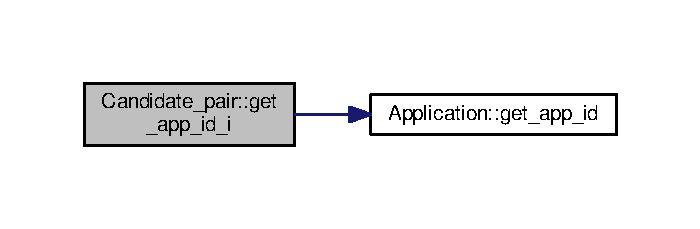
\includegraphics[width=336pt]{classCandidate__pair_a8fcc74d1e2ad95ab0ecb483a2ceb39b0_cgraph}
\end{center}
\end{figure}


\hypertarget{classCandidate__pair_aaee11e17681cfe95daed61e23b3bd6dc}{\index{Candidate\-\_\-pair@{Candidate\-\_\-pair}!get\-\_\-app\-\_\-id\-\_\-j@{get\-\_\-app\-\_\-id\-\_\-j}}
\index{get\-\_\-app\-\_\-id\-\_\-j@{get\-\_\-app\-\_\-id\-\_\-j}!Candidate_pair@{Candidate\-\_\-pair}}
\subsubsection[{get\-\_\-app\-\_\-id\-\_\-j}]{\setlength{\rightskip}{0pt plus 5cm}const std\-::string Candidate\-\_\-pair\-::get\-\_\-app\-\_\-id\-\_\-j (
\begin{DoxyParamCaption}
{}
\end{DoxyParamCaption}
)\hspace{0.3cm}{\ttfamily [inline]}}}\label{classCandidate__pair_aaee11e17681cfe95daed61e23b3bd6dc}


Here is the call graph for this function\-:
\nopagebreak
\begin{figure}[H]
\begin{center}
\leavevmode
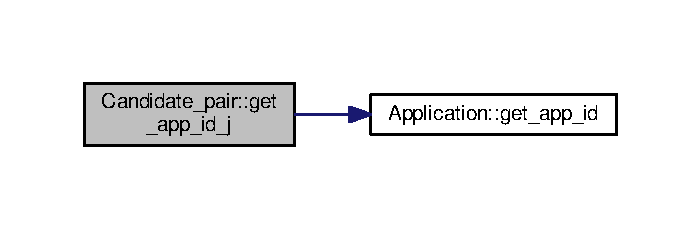
\includegraphics[width=336pt]{classCandidate__pair_aaee11e17681cfe95daed61e23b3bd6dc_cgraph}
\end{center}
\end{figure}


\hypertarget{classCandidate__pair_a68d1dec30fcbfd265355a980c0d01d63}{\index{Candidate\-\_\-pair@{Candidate\-\_\-pair}!get\-\_\-app\-\_\-j@{get\-\_\-app\-\_\-j}}
\index{get\-\_\-app\-\_\-j@{get\-\_\-app\-\_\-j}!Candidate_pair@{Candidate\-\_\-pair}}
\subsubsection[{get\-\_\-app\-\_\-j}]{\setlength{\rightskip}{0pt plus 5cm}{\bf Application} Candidate\-\_\-pair\-::get\-\_\-app\-\_\-j (
\begin{DoxyParamCaption}
{}
\end{DoxyParamCaption}
)\hspace{0.3cm}{\ttfamily [inline]}}}\label{classCandidate__pair_a68d1dec30fcbfd265355a980c0d01d63}
\hypertarget{classCandidate__pair_ae322ed41aa4660ba68d272a4c1d7f9f9}{\index{Candidate\-\_\-pair@{Candidate\-\_\-pair}!get\-\_\-app\-\_\-j\-\_\-ref@{get\-\_\-app\-\_\-j\-\_\-ref}}
\index{get\-\_\-app\-\_\-j\-\_\-ref@{get\-\_\-app\-\_\-j\-\_\-ref}!Candidate_pair@{Candidate\-\_\-pair}}
\subsubsection[{get\-\_\-app\-\_\-j\-\_\-ref}]{\setlength{\rightskip}{0pt plus 5cm}{\bf Application}\& Candidate\-\_\-pair\-::get\-\_\-app\-\_\-j\-\_\-ref (
\begin{DoxyParamCaption}
{}
\end{DoxyParamCaption}
)\hspace{0.3cm}{\ttfamily [inline]}}}\label{classCandidate__pair_ae322ed41aa4660ba68d272a4c1d7f9f9}
\hypertarget{classCandidate__pair_a82a48babd2f32c73e1f167d54e8c6ebd}{\index{Candidate\-\_\-pair@{Candidate\-\_\-pair}!get\-\_\-base\-\_\-fo\-\_\-i@{get\-\_\-base\-\_\-fo\-\_\-i}}
\index{get\-\_\-base\-\_\-fo\-\_\-i@{get\-\_\-base\-\_\-fo\-\_\-i}!Candidate_pair@{Candidate\-\_\-pair}}
\subsubsection[{get\-\_\-base\-\_\-fo\-\_\-i}]{\setlength{\rightskip}{0pt plus 5cm}const double Candidate\-\_\-pair\-::get\-\_\-base\-\_\-fo\-\_\-i (
\begin{DoxyParamCaption}
{}
\end{DoxyParamCaption}
)\hspace{0.3cm}{\ttfamily [inline]}}}\label{classCandidate__pair_a82a48babd2f32c73e1f167d54e8c6ebd}


Here is the call graph for this function\-:
\nopagebreak
\begin{figure}[H]
\begin{center}
\leavevmode
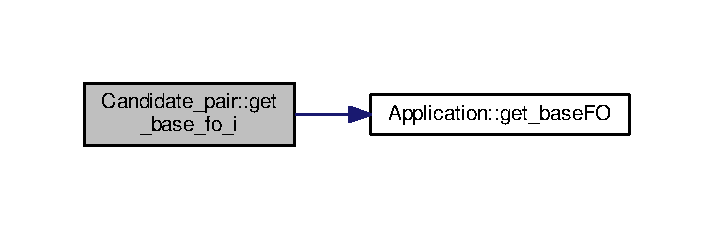
\includegraphics[width=342pt]{classCandidate__pair_a82a48babd2f32c73e1f167d54e8c6ebd_cgraph}
\end{center}
\end{figure}


\hypertarget{classCandidate__pair_a3f36cbb93291e8a72a6b3e88737d2a85}{\index{Candidate\-\_\-pair@{Candidate\-\_\-pair}!get\-\_\-base\-\_\-fo\-\_\-j@{get\-\_\-base\-\_\-fo\-\_\-j}}
\index{get\-\_\-base\-\_\-fo\-\_\-j@{get\-\_\-base\-\_\-fo\-\_\-j}!Candidate_pair@{Candidate\-\_\-pair}}
\subsubsection[{get\-\_\-base\-\_\-fo\-\_\-j}]{\setlength{\rightskip}{0pt plus 5cm}const double Candidate\-\_\-pair\-::get\-\_\-base\-\_\-fo\-\_\-j (
\begin{DoxyParamCaption}
{}
\end{DoxyParamCaption}
)\hspace{0.3cm}{\ttfamily [inline]}}}\label{classCandidate__pair_a3f36cbb93291e8a72a6b3e88737d2a85}


Here is the call graph for this function\-:
\nopagebreak
\begin{figure}[H]
\begin{center}
\leavevmode
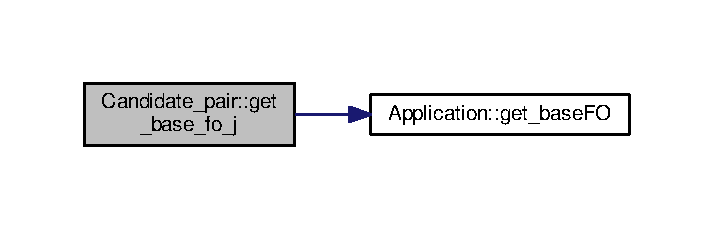
\includegraphics[width=342pt]{classCandidate__pair_a3f36cbb93291e8a72a6b3e88737d2a85_cgraph}
\end{center}
\end{figure}


\hypertarget{classCandidate__pair_a98ed7825fa11908514e7cfcc99013e4a}{\index{Candidate\-\_\-pair@{Candidate\-\_\-pair}!get\-\_\-current\-Cores\-\_\-d\-\_\-i@{get\-\_\-current\-Cores\-\_\-d\-\_\-i}}
\index{get\-\_\-current\-Cores\-\_\-d\-\_\-i@{get\-\_\-current\-Cores\-\_\-d\-\_\-i}!Candidate_pair@{Candidate\-\_\-pair}}
\subsubsection[{get\-\_\-current\-Cores\-\_\-d\-\_\-i}]{\setlength{\rightskip}{0pt plus 5cm}const int Candidate\-\_\-pair\-::get\-\_\-current\-Cores\-\_\-d\-\_\-i (
\begin{DoxyParamCaption}
{}
\end{DoxyParamCaption}
)\hspace{0.3cm}{\ttfamily [inline]}}}\label{classCandidate__pair_a98ed7825fa11908514e7cfcc99013e4a}


Here is the call graph for this function\-:
\nopagebreak
\begin{figure}[H]
\begin{center}
\leavevmode
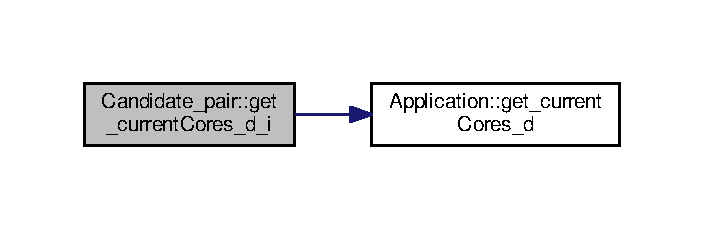
\includegraphics[width=338pt]{classCandidate__pair_a98ed7825fa11908514e7cfcc99013e4a_cgraph}
\end{center}
\end{figure}


\hypertarget{classCandidate__pair_a6e597198ca612c1d3c610edb38b395a0}{\index{Candidate\-\_\-pair@{Candidate\-\_\-pair}!get\-\_\-current\-Cores\-\_\-d\-\_\-j@{get\-\_\-current\-Cores\-\_\-d\-\_\-j}}
\index{get\-\_\-current\-Cores\-\_\-d\-\_\-j@{get\-\_\-current\-Cores\-\_\-d\-\_\-j}!Candidate_pair@{Candidate\-\_\-pair}}
\subsubsection[{get\-\_\-current\-Cores\-\_\-d\-\_\-j}]{\setlength{\rightskip}{0pt plus 5cm}const int Candidate\-\_\-pair\-::get\-\_\-current\-Cores\-\_\-d\-\_\-j (
\begin{DoxyParamCaption}
{}
\end{DoxyParamCaption}
)\hspace{0.3cm}{\ttfamily [inline]}}}\label{classCandidate__pair_a6e597198ca612c1d3c610edb38b395a0}


Here is the call graph for this function\-:
\nopagebreak
\begin{figure}[H]
\begin{center}
\leavevmode
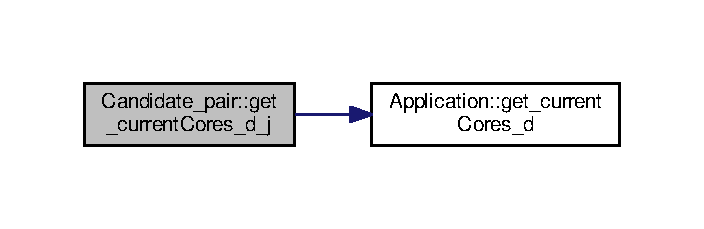
\includegraphics[width=338pt]{classCandidate__pair_a6e597198ca612c1d3c610edb38b395a0_cgraph}
\end{center}
\end{figure}


\hypertarget{classCandidate__pair_a4d45f63a1ffc4d420b28e88ae7e1dc99}{\index{Candidate\-\_\-pair@{Candidate\-\_\-pair}!get\-\_\-delta\-\_\-fo@{get\-\_\-delta\-\_\-fo}}
\index{get\-\_\-delta\-\_\-fo@{get\-\_\-delta\-\_\-fo}!Candidate_pair@{Candidate\-\_\-pair}}
\subsubsection[{get\-\_\-delta\-\_\-fo}]{\setlength{\rightskip}{0pt plus 5cm}const double Candidate\-\_\-pair\-::get\-\_\-delta\-\_\-fo (
\begin{DoxyParamCaption}
{}
\end{DoxyParamCaption}
)\hspace{0.3cm}{\ttfamily [inline]}}}\label{classCandidate__pair_a4d45f63a1ffc4d420b28e88ae7e1dc99}
\hypertarget{classCandidate__pair_a986854ee106c5d7cb64a7ab1161963f2}{\index{Candidate\-\_\-pair@{Candidate\-\_\-pair}!get\-\_\-new\-\_\-core\-\_\-assignment\-\_\-i@{get\-\_\-new\-\_\-core\-\_\-assignment\-\_\-i}}
\index{get\-\_\-new\-\_\-core\-\_\-assignment\-\_\-i@{get\-\_\-new\-\_\-core\-\_\-assignment\-\_\-i}!Candidate_pair@{Candidate\-\_\-pair}}
\subsubsection[{get\-\_\-new\-\_\-core\-\_\-assignment\-\_\-i}]{\setlength{\rightskip}{0pt plus 5cm}const int Candidate\-\_\-pair\-::get\-\_\-new\-\_\-core\-\_\-assignment\-\_\-i (
\begin{DoxyParamCaption}
{}
\end{DoxyParamCaption}
)\hspace{0.3cm}{\ttfamily [inline]}}}\label{classCandidate__pair_a986854ee106c5d7cb64a7ab1161963f2}
\hypertarget{classCandidate__pair_ab008e2c787a8ee44ab0102a280d9bea6}{\index{Candidate\-\_\-pair@{Candidate\-\_\-pair}!get\-\_\-new\-\_\-core\-\_\-assignment\-\_\-j@{get\-\_\-new\-\_\-core\-\_\-assignment\-\_\-j}}
\index{get\-\_\-new\-\_\-core\-\_\-assignment\-\_\-j@{get\-\_\-new\-\_\-core\-\_\-assignment\-\_\-j}!Candidate_pair@{Candidate\-\_\-pair}}
\subsubsection[{get\-\_\-new\-\_\-core\-\_\-assignment\-\_\-j}]{\setlength{\rightskip}{0pt plus 5cm}const int Candidate\-\_\-pair\-::get\-\_\-new\-\_\-core\-\_\-assignment\-\_\-j (
\begin{DoxyParamCaption}
{}
\end{DoxyParamCaption}
)\hspace{0.3cm}{\ttfamily [inline]}}}\label{classCandidate__pair_ab008e2c787a8ee44ab0102a280d9bea6}
\hypertarget{classCandidate__pair_a829335d66b073892cba3a89a90a9c5c8}{\index{Candidate\-\_\-pair@{Candidate\-\_\-pair}!get\-\_\-real\-\_\-i@{get\-\_\-real\-\_\-i}}
\index{get\-\_\-real\-\_\-i@{get\-\_\-real\-\_\-i}!Candidate_pair@{Candidate\-\_\-pair}}
\subsubsection[{get\-\_\-real\-\_\-i}]{\setlength{\rightskip}{0pt plus 5cm}double Candidate\-\_\-pair\-::get\-\_\-real\-\_\-i (
\begin{DoxyParamCaption}
{}
\end{DoxyParamCaption}
)\hspace{0.3cm}{\ttfamily [inline]}}}\label{classCandidate__pair_a829335d66b073892cba3a89a90a9c5c8}
\hypertarget{classCandidate__pair_af2dc9a093dced6724b85018cfdb307cd}{\index{Candidate\-\_\-pair@{Candidate\-\_\-pair}!get\-\_\-real\-\_\-j@{get\-\_\-real\-\_\-j}}
\index{get\-\_\-real\-\_\-j@{get\-\_\-real\-\_\-j}!Candidate_pair@{Candidate\-\_\-pair}}
\subsubsection[{get\-\_\-real\-\_\-j}]{\setlength{\rightskip}{0pt plus 5cm}double Candidate\-\_\-pair\-::get\-\_\-real\-\_\-j (
\begin{DoxyParamCaption}
{}
\end{DoxyParamCaption}
)\hspace{0.3cm}{\ttfamily [inline]}}}\label{classCandidate__pair_af2dc9a093dced6724b85018cfdb307cd}
\hypertarget{classCandidate__pair_a3d7cb54ffabff340b583925427424085}{\index{Candidate\-\_\-pair@{Candidate\-\_\-pair}!get\-\_\-session\-\_\-app\-\_\-id\-\_\-i@{get\-\_\-session\-\_\-app\-\_\-id\-\_\-i}}
\index{get\-\_\-session\-\_\-app\-\_\-id\-\_\-i@{get\-\_\-session\-\_\-app\-\_\-id\-\_\-i}!Candidate_pair@{Candidate\-\_\-pair}}
\subsubsection[{get\-\_\-session\-\_\-app\-\_\-id\-\_\-i}]{\setlength{\rightskip}{0pt plus 5cm}const std\-::string Candidate\-\_\-pair\-::get\-\_\-session\-\_\-app\-\_\-id\-\_\-i (
\begin{DoxyParamCaption}
{}
\end{DoxyParamCaption}
)\hspace{0.3cm}{\ttfamily [inline]}}}\label{classCandidate__pair_a3d7cb54ffabff340b583925427424085}


Here is the call graph for this function\-:
\nopagebreak
\begin{figure}[H]
\begin{center}
\leavevmode
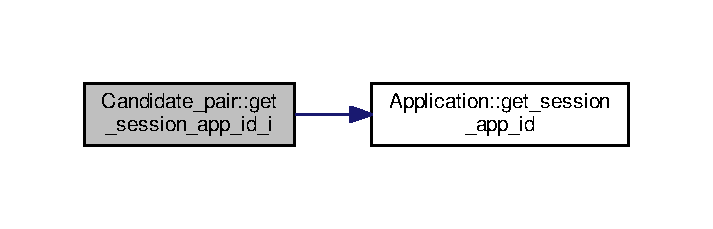
\includegraphics[width=342pt]{classCandidate__pair_a3d7cb54ffabff340b583925427424085_cgraph}
\end{center}
\end{figure}


\hypertarget{classCandidate__pair_a8e2faa0c4a09de7667d760a7de0b9596}{\index{Candidate\-\_\-pair@{Candidate\-\_\-pair}!get\-\_\-session\-\_\-app\-\_\-id\-\_\-j@{get\-\_\-session\-\_\-app\-\_\-id\-\_\-j}}
\index{get\-\_\-session\-\_\-app\-\_\-id\-\_\-j@{get\-\_\-session\-\_\-app\-\_\-id\-\_\-j}!Candidate_pair@{Candidate\-\_\-pair}}
\subsubsection[{get\-\_\-session\-\_\-app\-\_\-id\-\_\-j}]{\setlength{\rightskip}{0pt plus 5cm}const std\-::string Candidate\-\_\-pair\-::get\-\_\-session\-\_\-app\-\_\-id\-\_\-j (
\begin{DoxyParamCaption}
{}
\end{DoxyParamCaption}
)\hspace{0.3cm}{\ttfamily [inline]}}}\label{classCandidate__pair_a8e2faa0c4a09de7667d760a7de0b9596}


Here is the call graph for this function\-:
\nopagebreak
\begin{figure}[H]
\begin{center}
\leavevmode
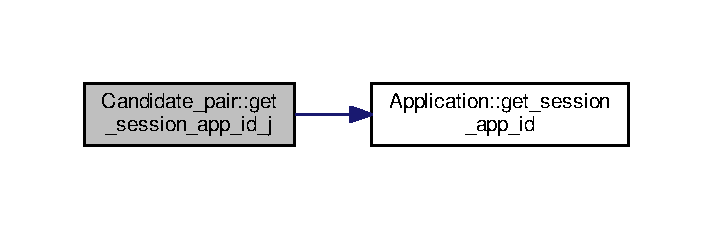
\includegraphics[width=342pt]{classCandidate__pair_a8e2faa0c4a09de7667d760a7de0b9596_cgraph}
\end{center}
\end{figure}


\hypertarget{classCandidate__pair_aee6e0ca68882feefe44c6f095961a8d7}{\index{Candidate\-\_\-pair@{Candidate\-\_\-pair}!set\-\_\-real\-\_\-i@{set\-\_\-real\-\_\-i}}
\index{set\-\_\-real\-\_\-i@{set\-\_\-real\-\_\-i}!Candidate_pair@{Candidate\-\_\-pair}}
\subsubsection[{set\-\_\-real\-\_\-i}]{\setlength{\rightskip}{0pt plus 5cm}void Candidate\-\_\-pair\-::set\-\_\-real\-\_\-i (
\begin{DoxyParamCaption}
\item[{double}]{d}
\end{DoxyParamCaption}
)\hspace{0.3cm}{\ttfamily [inline]}}}\label{classCandidate__pair_aee6e0ca68882feefe44c6f095961a8d7}
\hypertarget{classCandidate__pair_a9277d72b649e1cdd857fcb42d6926da1}{\index{Candidate\-\_\-pair@{Candidate\-\_\-pair}!set\-\_\-real\-\_\-j@{set\-\_\-real\-\_\-j}}
\index{set\-\_\-real\-\_\-j@{set\-\_\-real\-\_\-j}!Candidate_pair@{Candidate\-\_\-pair}}
\subsubsection[{set\-\_\-real\-\_\-j}]{\setlength{\rightskip}{0pt plus 5cm}void Candidate\-\_\-pair\-::set\-\_\-real\-\_\-j (
\begin{DoxyParamCaption}
\item[{double}]{d}
\end{DoxyParamCaption}
)\hspace{0.3cm}{\ttfamily [inline]}}}\label{classCandidate__pair_a9277d72b649e1cdd857fcb42d6926da1}


\subsection{Member Data Documentation}
\hypertarget{classCandidate__pair_acc570b14122b1f3cbc0e5440778cd4d8}{\index{Candidate\-\_\-pair@{Candidate\-\_\-pair}!app\-\_\-i@{app\-\_\-i}}
\index{app\-\_\-i@{app\-\_\-i}!Candidate_pair@{Candidate\-\_\-pair}}
\subsubsection[{app\-\_\-i}]{\setlength{\rightskip}{0pt plus 5cm}{\bf Application} Candidate\-\_\-pair\-::app\-\_\-i\hspace{0.3cm}{\ttfamily [private]}}}\label{classCandidate__pair_acc570b14122b1f3cbc0e5440778cd4d8}


Copy of the first \hyperlink{classApplication}{Application}. 

\hypertarget{classCandidate__pair_a7497fbea2f53cb71a01486e2b655880e}{\index{Candidate\-\_\-pair@{Candidate\-\_\-pair}!app\-\_\-j@{app\-\_\-j}}
\index{app\-\_\-j@{app\-\_\-j}!Candidate_pair@{Candidate\-\_\-pair}}
\subsubsection[{app\-\_\-j}]{\setlength{\rightskip}{0pt plus 5cm}{\bf Application} Candidate\-\_\-pair\-::app\-\_\-j\hspace{0.3cm}{\ttfamily [private]}}}\label{classCandidate__pair_a7497fbea2f53cb71a01486e2b655880e}


Copy of the second \hyperlink{classApplication}{Application}. 

\hypertarget{classCandidate__pair_a190b95c0ee800a6b37fec8f5d84c62c6}{\index{Candidate\-\_\-pair@{Candidate\-\_\-pair}!delta\-\_\-fo@{delta\-\_\-fo}}
\index{delta\-\_\-fo@{delta\-\_\-fo}!Candidate_pair@{Candidate\-\_\-pair}}
\subsubsection[{delta\-\_\-fo}]{\setlength{\rightskip}{0pt plus 5cm}double Candidate\-\_\-pair\-::delta\-\_\-fo\hspace{0.3cm}{\ttfamily [private]}}}\label{classCandidate__pair_a190b95c0ee800a6b37fec8f5d84c62c6}


Delta Objective Function following the move. 

\hypertarget{classCandidate__pair_af9ed12a88dc27e921764feea5d1369f1}{\index{Candidate\-\_\-pair@{Candidate\-\_\-pair}!delta\-\_\-i@{delta\-\_\-i}}
\index{delta\-\_\-i@{delta\-\_\-i}!Candidate_pair@{Candidate\-\_\-pair}}
\subsubsection[{delta\-\_\-i}]{\setlength{\rightskip}{0pt plus 5cm}int Candidate\-\_\-pair\-::delta\-\_\-i\hspace{0.3cm}{\ttfamily [private]}}}\label{classCandidate__pair_af9ed12a88dc27e921764feea5d1369f1}


Delta cores following the move (first application) 

\hypertarget{classCandidate__pair_a65cec47eee407768393199d82f1eebe4}{\index{Candidate\-\_\-pair@{Candidate\-\_\-pair}!delta\-\_\-j@{delta\-\_\-j}}
\index{delta\-\_\-j@{delta\-\_\-j}!Candidate_pair@{Candidate\-\_\-pair}}
\subsubsection[{delta\-\_\-j}]{\setlength{\rightskip}{0pt plus 5cm}int Candidate\-\_\-pair\-::delta\-\_\-j\hspace{0.3cm}{\ttfamily [private]}}}\label{classCandidate__pair_a65cec47eee407768393199d82f1eebe4}


Delta cores following the move (second application) 

\hypertarget{classCandidate__pair_a8ede26b1a4d583b2b9ac360612c789bf}{\index{Candidate\-\_\-pair@{Candidate\-\_\-pair}!new\-\_\-core\-\_\-assignment\-\_\-i@{new\-\_\-core\-\_\-assignment\-\_\-i}}
\index{new\-\_\-core\-\_\-assignment\-\_\-i@{new\-\_\-core\-\_\-assignment\-\_\-i}!Candidate_pair@{Candidate\-\_\-pair}}
\subsubsection[{new\-\_\-core\-\_\-assignment\-\_\-i}]{\setlength{\rightskip}{0pt plus 5cm}int Candidate\-\_\-pair\-::new\-\_\-core\-\_\-assignment\-\_\-i\hspace{0.3cm}{\ttfamily [private]}}}\label{classCandidate__pair_a8ede26b1a4d583b2b9ac360612c789bf}


Cores after the move (first application) 

\hypertarget{classCandidate__pair_ab4d273d1e72ae26d5230f4d783ef745b}{\index{Candidate\-\_\-pair@{Candidate\-\_\-pair}!new\-\_\-core\-\_\-assignment\-\_\-j@{new\-\_\-core\-\_\-assignment\-\_\-j}}
\index{new\-\_\-core\-\_\-assignment\-\_\-j@{new\-\_\-core\-\_\-assignment\-\_\-j}!Candidate_pair@{Candidate\-\_\-pair}}
\subsubsection[{new\-\_\-core\-\_\-assignment\-\_\-j}]{\setlength{\rightskip}{0pt plus 5cm}int Candidate\-\_\-pair\-::new\-\_\-core\-\_\-assignment\-\_\-j\hspace{0.3cm}{\ttfamily [private]}}}\label{classCandidate__pair_ab4d273d1e72ae26d5230f4d783ef745b}


Cores after the move (second application) 

\hypertarget{classCandidate__pair_a8ac003373540c4149eaa8db2392921e0}{\index{Candidate\-\_\-pair@{Candidate\-\_\-pair}!real\-\_\-i@{real\-\_\-i}}
\index{real\-\_\-i@{real\-\_\-i}!Candidate_pair@{Candidate\-\_\-pair}}
\subsubsection[{real\-\_\-i}]{\setlength{\rightskip}{0pt plus 5cm}double Candidate\-\_\-pair\-::real\-\_\-i\hspace{0.3cm}{\ttfamily [private]}}}\label{classCandidate__pair_a8ac003373540c4149eaa8db2392921e0}


Real predictor value calculated (M\-P\-I) after the interpolation (first application) 

\hypertarget{classCandidate__pair_ad1096cd9230ebca7f706981dee48794c}{\index{Candidate\-\_\-pair@{Candidate\-\_\-pair}!real\-\_\-j@{real\-\_\-j}}
\index{real\-\_\-j@{real\-\_\-j}!Candidate_pair@{Candidate\-\_\-pair}}
\subsubsection[{real\-\_\-j}]{\setlength{\rightskip}{0pt plus 5cm}double Candidate\-\_\-pair\-::real\-\_\-j\hspace{0.3cm}{\ttfamily [private]}}}\label{classCandidate__pair_ad1096cd9230ebca7f706981dee48794c}


Real predictor value calculated (M\-P\-I) after the interpolation (second application) 



The documentation for this class was generated from the following file\-:\begin{DoxyCompactItemize}
\item 
/vagrant/\-P\-R\-O\-J\-E\-C\-T\-\_\-\-S\-P\-A\-R\-K/\-P\-A\-C\-S\-\_\-\-P\-R\-O\-J\-E\-C\-T/opt\-\_\-jr/src/\hyperlink{candidate__pair_8hh}{candidate\-\_\-pair.\-hh}\end{DoxyCompactItemize}

\hypertarget{classCandidates}{\section{Candidates Class Reference}
\label{classCandidates}\index{Candidates@{Candidates}}
}


{\ttfamily \#include $<$candidates.\-hh$>$}



Collaboration diagram for Candidates\-:
\nopagebreak
\begin{figure}[H]
\begin{center}
\leavevmode
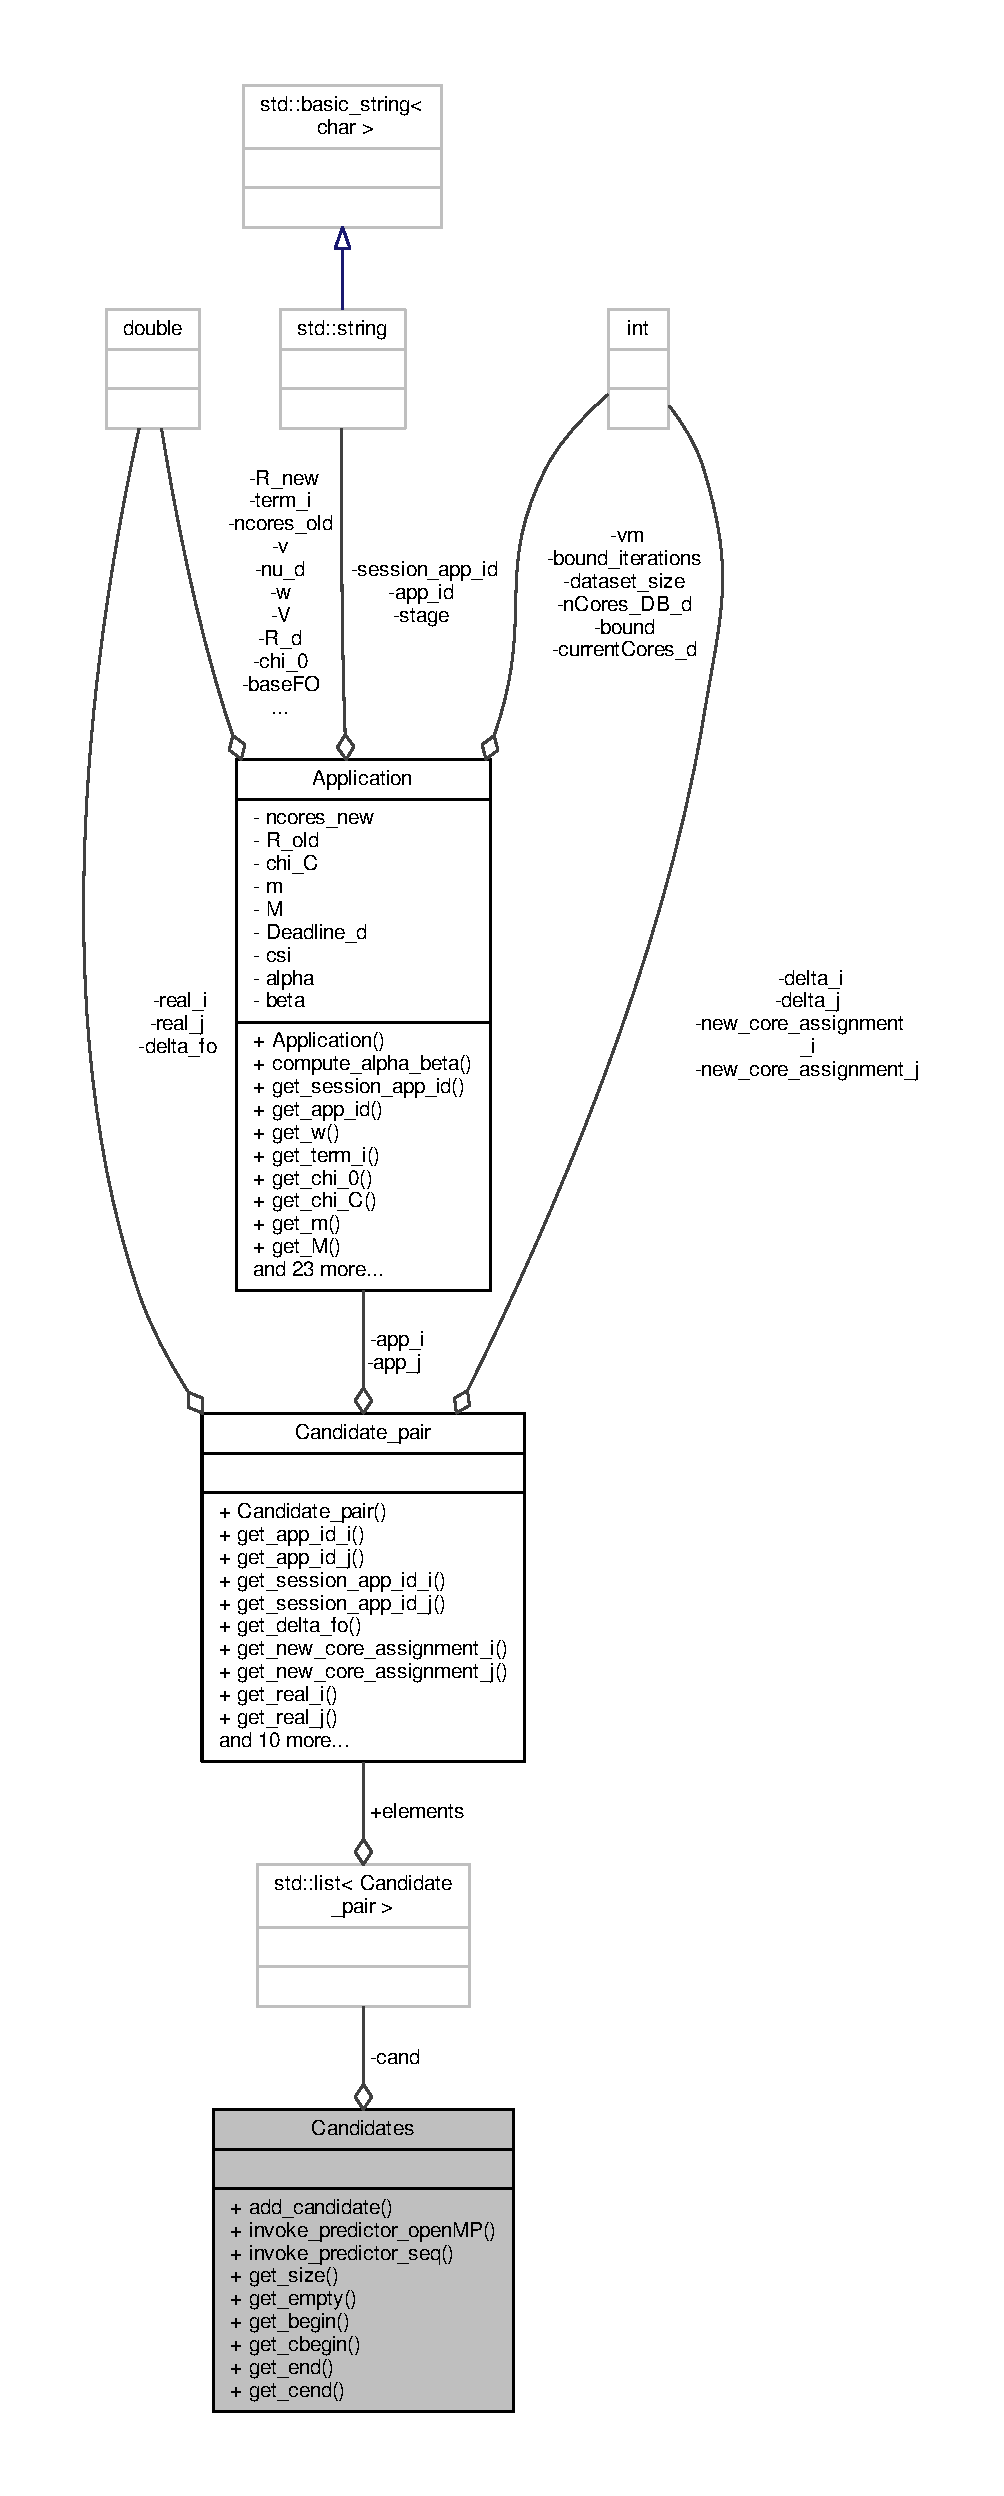
\includegraphics[height=550pt]{classCandidates__coll__graph}
\end{center}
\end{figure}
\subsection*{Public Member Functions}
\begin{DoxyCompactItemize}
\item 
void \hyperlink{classCandidates_ad76cf8f7ae979cc49afd67b5fc9c702b}{add\-\_\-candidate} (\hyperlink{classApplication}{Application} app\-\_\-i, \hyperlink{classApplication}{Application} app\-\_\-j, int contr1, int contr2, double delta, double delta\-\_\-i, double delta\-\_\-j)
\item 
void \hyperlink{classCandidates_a9cc75e29ad2d0f2eb29fae2801c8e58b}{invoke\-\_\-predictor\-\_\-open\-M\-P} (\hyperlink{classOpt__jr__parameters}{Opt\-\_\-jr\-\_\-parameters} \&par, \hyperlink{classConfiguration}{Configuration} \&configuration)
\item 
void \hyperlink{classCandidates_a0f5bfe459063108d80ed8dce02c6c07b}{invoke\-\_\-predictor\-\_\-seq} (M\-Y\-S\-Q\-L $\ast$conn, \hyperlink{classOpt__jr__parameters}{Opt\-\_\-jr\-\_\-parameters} \&par, \hyperlink{classConfiguration}{Configuration} \&configuration)
\item 
int \hyperlink{classCandidates_ac10d9fe35730800bacac1d89ab117a4c}{get\-\_\-size} ()
\item 
bool \hyperlink{classCandidates_aaba3941ba950a669776a1e53fb710691}{get\-\_\-empty} ()
\item 
std\-::list$<$ \hyperlink{classCandidate__pair}{Candidate\-\_\-pair} $>$\\*
\-::iterator \hyperlink{classCandidates_a69a3001a09b54813959d2b44662f7f18}{get\-\_\-begin} ()
\item 
std\-::list$<$ \hyperlink{classCandidate__pair}{Candidate\-\_\-pair} $>$\\*
\-::const\-\_\-iterator \hyperlink{classCandidates_a9fb1fe0a56d70f0f0f4243cd7e32448a}{get\-\_\-cbegin} ()
\item 
std\-::list$<$ \hyperlink{classCandidate__pair}{Candidate\-\_\-pair} $>$\\*
\-::iterator \hyperlink{classCandidates_ad763ac469728621a81010ca7c14b4246}{get\-\_\-end} ()
\item 
std\-::list$<$ \hyperlink{classCandidate__pair}{Candidate\-\_\-pair} $>$\\*
\-::const\-\_\-iterator \hyperlink{classCandidates_a4c865dc532a6ead85200c7b66434bf71}{get\-\_\-cend} ()
\end{DoxyCompactItemize}
\subsection*{Private Attributes}
\begin{DoxyCompactItemize}
\item 
std\-::list$<$ \hyperlink{classCandidate__pair}{Candidate\-\_\-pair} $>$ \hyperlink{classCandidates_a45b43ae5f71d2162f591e4019f1bc560}{cand}
\end{DoxyCompactItemize}


\subsection{Detailed Description}
Auxiliary class used by local\-\_\-search; it stores pairs of applications for which a cores exchange could be profitable and provide methods to add \hyperlink{classCandidate__pair}{Candidate\-\_\-pair} and evaluate in parallel the objective function 

\subsection{Member Function Documentation}
\hypertarget{classCandidates_ad76cf8f7ae979cc49afd67b5fc9c702b}{\index{Candidates@{Candidates}!add\-\_\-candidate@{add\-\_\-candidate}}
\index{add\-\_\-candidate@{add\-\_\-candidate}!Candidates@{Candidates}}
\subsubsection[{add\-\_\-candidate}]{\setlength{\rightskip}{0pt plus 5cm}void Candidates\-::add\-\_\-candidate (
\begin{DoxyParamCaption}
\item[{{\bf Application}}]{app\-\_\-i, }
\item[{{\bf Application}}]{app\-\_\-j, }
\item[{int}]{contr1, }
\item[{int}]{contr2, }
\item[{double}]{delta, }
\item[{double}]{delta\-\_\-i, }
\item[{double}]{delta\-\_\-j}
\end{DoxyParamCaption}
)}}\label{classCandidates_ad76cf8f7ae979cc49afd67b5fc9c702b}
\char`\"{}add\-\_\-candidate\char`\"{} build a \char`\"{}\-Candidate\-\_\-pair\char`\"{} object and stores it in a \hyperlink{classCandidates}{Candidates} container ordered by increasing delta F\-O 

Here is the caller graph for this function\-:
\nopagebreak
\begin{figure}[H]
\begin{center}
\leavevmode
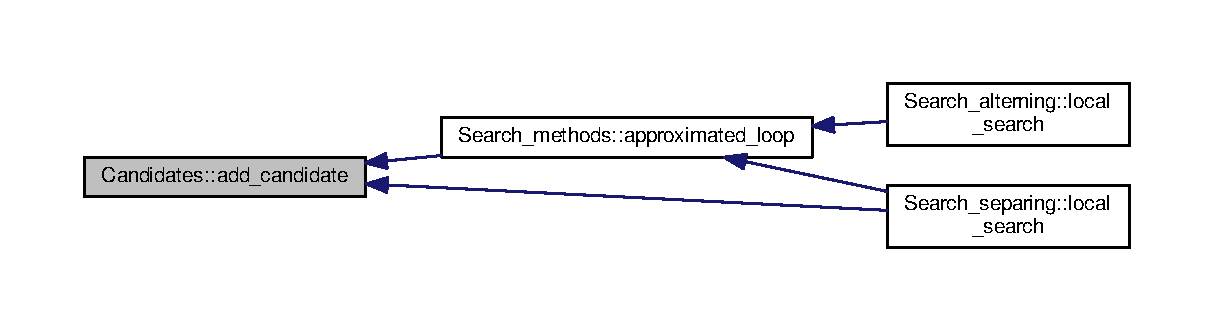
\includegraphics[width=350pt]{classCandidates_ad76cf8f7ae979cc49afd67b5fc9c702b_icgraph}
\end{center}
\end{figure}


\hypertarget{classCandidates_a69a3001a09b54813959d2b44662f7f18}{\index{Candidates@{Candidates}!get\-\_\-begin@{get\-\_\-begin}}
\index{get\-\_\-begin@{get\-\_\-begin}!Candidates@{Candidates}}
\subsubsection[{get\-\_\-begin}]{\setlength{\rightskip}{0pt plus 5cm}std\-::list$<${\bf Candidate\-\_\-pair}$>$\-::iterator Candidates\-::get\-\_\-begin (
\begin{DoxyParamCaption}
{}
\end{DoxyParamCaption}
)\hspace{0.3cm}{\ttfamily [inline]}}}\label{classCandidates_a69a3001a09b54813959d2b44662f7f18}


Here is the caller graph for this function\-:
\nopagebreak
\begin{figure}[H]
\begin{center}
\leavevmode
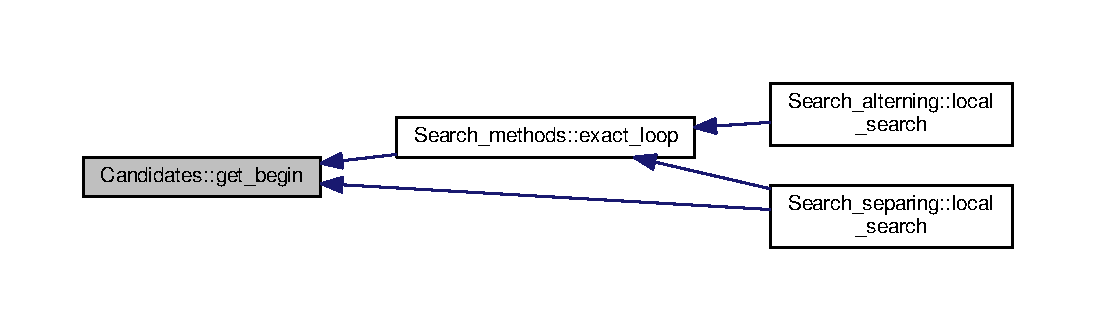
\includegraphics[width=350pt]{classCandidates_a69a3001a09b54813959d2b44662f7f18_icgraph}
\end{center}
\end{figure}


\hypertarget{classCandidates_a9fb1fe0a56d70f0f0f4243cd7e32448a}{\index{Candidates@{Candidates}!get\-\_\-cbegin@{get\-\_\-cbegin}}
\index{get\-\_\-cbegin@{get\-\_\-cbegin}!Candidates@{Candidates}}
\subsubsection[{get\-\_\-cbegin}]{\setlength{\rightskip}{0pt plus 5cm}std\-::list$<${\bf Candidate\-\_\-pair}$>$\-::const\-\_\-iterator Candidates\-::get\-\_\-cbegin (
\begin{DoxyParamCaption}
{}
\end{DoxyParamCaption}
)\hspace{0.3cm}{\ttfamily [inline]}}}\label{classCandidates_a9fb1fe0a56d70f0f0f4243cd7e32448a}
\hypertarget{classCandidates_a4c865dc532a6ead85200c7b66434bf71}{\index{Candidates@{Candidates}!get\-\_\-cend@{get\-\_\-cend}}
\index{get\-\_\-cend@{get\-\_\-cend}!Candidates@{Candidates}}
\subsubsection[{get\-\_\-cend}]{\setlength{\rightskip}{0pt plus 5cm}std\-::list$<${\bf Candidate\-\_\-pair}$>$\-::const\-\_\-iterator Candidates\-::get\-\_\-cend (
\begin{DoxyParamCaption}
{}
\end{DoxyParamCaption}
)\hspace{0.3cm}{\ttfamily [inline]}}}\label{classCandidates_a4c865dc532a6ead85200c7b66434bf71}
\hypertarget{classCandidates_aaba3941ba950a669776a1e53fb710691}{\index{Candidates@{Candidates}!get\-\_\-empty@{get\-\_\-empty}}
\index{get\-\_\-empty@{get\-\_\-empty}!Candidates@{Candidates}}
\subsubsection[{get\-\_\-empty}]{\setlength{\rightskip}{0pt plus 5cm}bool Candidates\-::get\-\_\-empty (
\begin{DoxyParamCaption}
{}
\end{DoxyParamCaption}
)\hspace{0.3cm}{\ttfamily [inline]}}}\label{classCandidates_aaba3941ba950a669776a1e53fb710691}


Here is the caller graph for this function\-:
\nopagebreak
\begin{figure}[H]
\begin{center}
\leavevmode
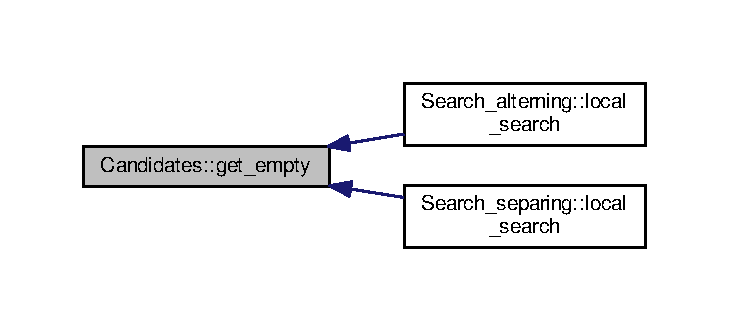
\includegraphics[width=350pt]{classCandidates_aaba3941ba950a669776a1e53fb710691_icgraph}
\end{center}
\end{figure}


\hypertarget{classCandidates_ad763ac469728621a81010ca7c14b4246}{\index{Candidates@{Candidates}!get\-\_\-end@{get\-\_\-end}}
\index{get\-\_\-end@{get\-\_\-end}!Candidates@{Candidates}}
\subsubsection[{get\-\_\-end}]{\setlength{\rightskip}{0pt plus 5cm}std\-::list$<${\bf Candidate\-\_\-pair}$>$\-::iterator Candidates\-::get\-\_\-end (
\begin{DoxyParamCaption}
{}
\end{DoxyParamCaption}
)\hspace{0.3cm}{\ttfamily [inline]}}}\label{classCandidates_ad763ac469728621a81010ca7c14b4246}


Here is the caller graph for this function\-:
\nopagebreak
\begin{figure}[H]
\begin{center}
\leavevmode
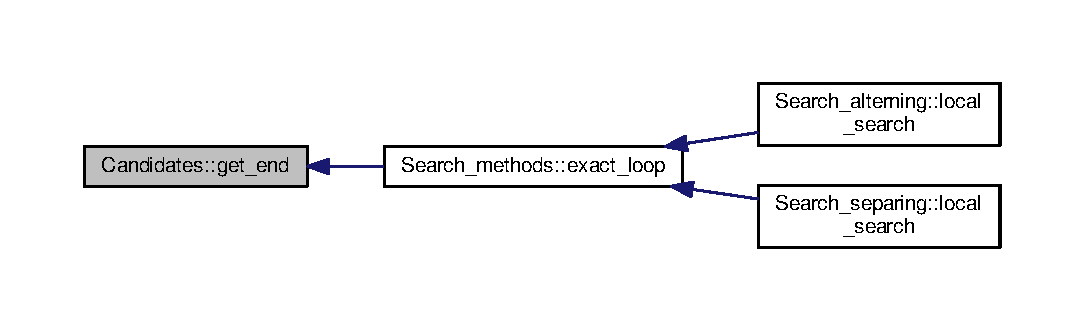
\includegraphics[width=350pt]{classCandidates_ad763ac469728621a81010ca7c14b4246_icgraph}
\end{center}
\end{figure}


\hypertarget{classCandidates_ac10d9fe35730800bacac1d89ab117a4c}{\index{Candidates@{Candidates}!get\-\_\-size@{get\-\_\-size}}
\index{get\-\_\-size@{get\-\_\-size}!Candidates@{Candidates}}
\subsubsection[{get\-\_\-size}]{\setlength{\rightskip}{0pt plus 5cm}int Candidates\-::get\-\_\-size (
\begin{DoxyParamCaption}
{}
\end{DoxyParamCaption}
)\hspace{0.3cm}{\ttfamily [inline]}}}\label{classCandidates_ac10d9fe35730800bacac1d89ab117a4c}


Here is the caller graph for this function\-:
\nopagebreak
\begin{figure}[H]
\begin{center}
\leavevmode
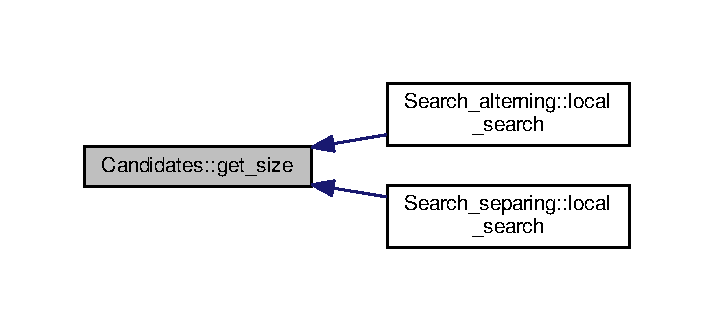
\includegraphics[width=342pt]{classCandidates_ac10d9fe35730800bacac1d89ab117a4c_icgraph}
\end{center}
\end{figure}


\hypertarget{classCandidates_a9cc75e29ad2d0f2eb29fae2801c8e58b}{\index{Candidates@{Candidates}!invoke\-\_\-predictor\-\_\-open\-M\-P@{invoke\-\_\-predictor\-\_\-open\-M\-P}}
\index{invoke\-\_\-predictor\-\_\-open\-M\-P@{invoke\-\_\-predictor\-\_\-open\-M\-P}!Candidates@{Candidates}}
\subsubsection[{invoke\-\_\-predictor\-\_\-open\-M\-P}]{\setlength{\rightskip}{0pt plus 5cm}void Candidates\-::invoke\-\_\-predictor\-\_\-open\-M\-P (
\begin{DoxyParamCaption}
\item[{{\bf Opt\-\_\-jr\-\_\-parameters} \&}]{par, }
\item[{{\bf Configuration} \&}]{configuration}
\end{DoxyParamCaption}
)}}\label{classCandidates_a9cc75e29ad2d0f2eb29fae2801c8e58b}
\char`\"{}invoke\-\_\-predictor\-\_\-open\-M\-P\char`\"{} calls in parallel the component for each pair of application and it stores the results for each pair in real\-\_\-i, real\-\_\-j. 

Here is the caller graph for this function\-:
\nopagebreak
\begin{figure}[H]
\begin{center}
\leavevmode
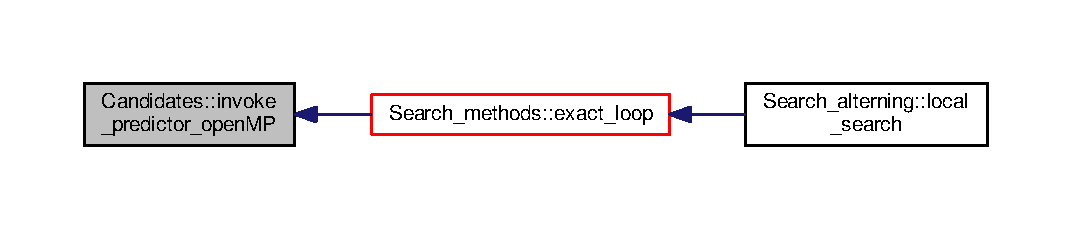
\includegraphics[width=350pt]{classCandidates_a9cc75e29ad2d0f2eb29fae2801c8e58b_icgraph}
\end{center}
\end{figure}


\hypertarget{classCandidates_a0f5bfe459063108d80ed8dce02c6c07b}{\index{Candidates@{Candidates}!invoke\-\_\-predictor\-\_\-seq@{invoke\-\_\-predictor\-\_\-seq}}
\index{invoke\-\_\-predictor\-\_\-seq@{invoke\-\_\-predictor\-\_\-seq}!Candidates@{Candidates}}
\subsubsection[{invoke\-\_\-predictor\-\_\-seq}]{\setlength{\rightskip}{0pt plus 5cm}void Candidates\-::invoke\-\_\-predictor\-\_\-seq (
\begin{DoxyParamCaption}
\item[{M\-Y\-S\-Q\-L $\ast$}]{conn, }
\item[{{\bf Opt\-\_\-jr\-\_\-parameters} \&}]{par, }
\item[{{\bf Configuration} \&}]{configuration}
\end{DoxyParamCaption}
)}}\label{classCandidates_a0f5bfe459063108d80ed8dce02c6c07b}
\char`\"{}invoke\-\_\-predictor\-\_\-seq\char`\"{} calls sequencially the component for each pair of application and it stores the results for each pair in real\-\_\-i, real\-\_\-j. 

Here is the caller graph for this function\-:
\nopagebreak
\begin{figure}[H]
\begin{center}
\leavevmode
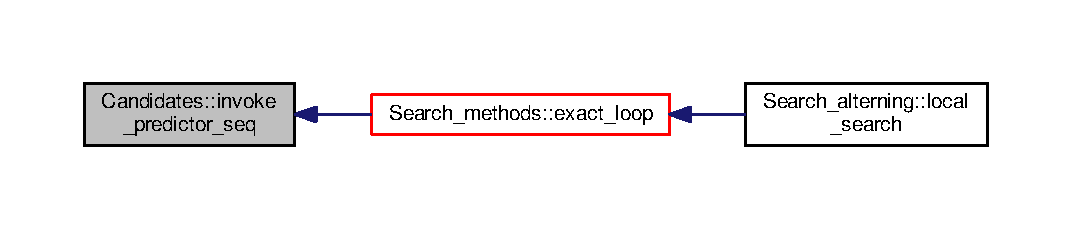
\includegraphics[width=350pt]{classCandidates_a0f5bfe459063108d80ed8dce02c6c07b_icgraph}
\end{center}
\end{figure}




\subsection{Member Data Documentation}
\hypertarget{classCandidates_a45b43ae5f71d2162f591e4019f1bc560}{\index{Candidates@{Candidates}!cand@{cand}}
\index{cand@{cand}!Candidates@{Candidates}}
\subsubsection[{cand}]{\setlength{\rightskip}{0pt plus 5cm}std\-::list$<${\bf Candidate\-\_\-pair}$>$ Candidates\-::cand\hspace{0.3cm}{\ttfamily [private]}}}\label{classCandidates_a45b43ae5f71d2162f591e4019f1bc560}
Container where applications candidates to change cores are stored in order of increasing delta\-F\-O 

The documentation for this class was generated from the following files\-:\begin{DoxyCompactItemize}
\item 
/vagrant/\-P\-R\-O\-J\-E\-C\-T\-\_\-\-S\-P\-A\-R\-K/\-P\-A\-C\-S\-\_\-\-P\-R\-O\-J\-E\-C\-T/opt\-\_\-jr/src/\hyperlink{candidates_8hh}{candidates.\-hh}\item 
/vagrant/\-P\-R\-O\-J\-E\-C\-T\-\_\-\-S\-P\-A\-R\-K/\-P\-A\-C\-S\-\_\-\-P\-R\-O\-J\-E\-C\-T/opt\-\_\-jr/src/\hyperlink{candidates_8cpp}{candidates.\-cpp}\end{DoxyCompactItemize}

\hypertarget{classConfiguration}{\section{Configuration Class Reference}
\label{classConfiguration}\index{Configuration@{Configuration}}
}


{\ttfamily \#include $<$configuration.\-hh$>$}



Collaboration diagram for Configuration\-:
\nopagebreak
\begin{figure}[H]
\begin{center}
\leavevmode
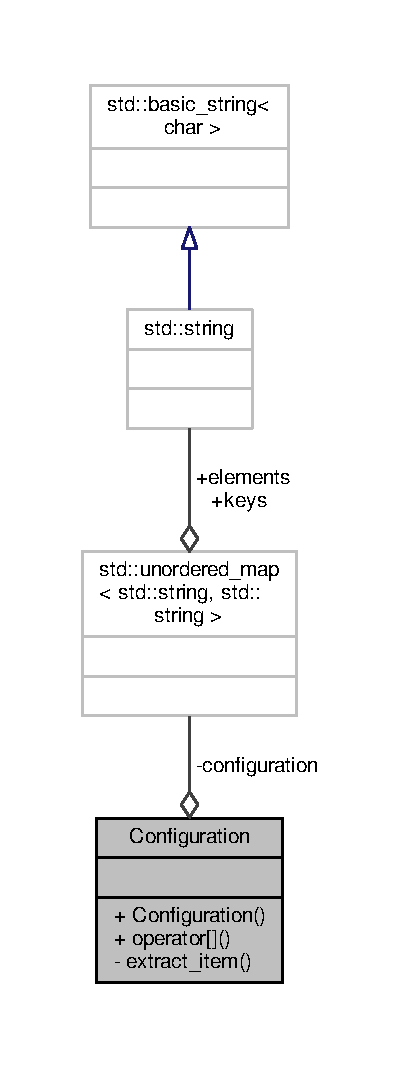
\includegraphics[width=193pt]{classConfiguration__coll__graph}
\end{center}
\end{figure}
\subsection*{Public Member Functions}
\begin{DoxyCompactItemize}
\item 
\hyperlink{classConfiguration_a779947337bf652f0e773cb29f37f14ba}{Configuration} ()
\item 
std\-::string \hyperlink{classConfiguration_ad01eea5b98871f1cc4dbf28b9fe92093}{operator\mbox{[}$\,$\mbox{]}} (std\-::string s)
\end{DoxyCompactItemize}
\subsection*{Private Member Functions}
\begin{DoxyCompactItemize}
\item 
char $\ast$ \hyperlink{classConfiguration_ac2ca184b014af7f7caa3ac487909a8f3}{extract\-\_\-item} (char $\ast$const string, char $\ast$const left, const char $\ast$const right)
\end{DoxyCompactItemize}
\subsection*{Private Attributes}
\begin{DoxyCompactItemize}
\item 
std\-::unordered\-\_\-map\\*
$<$ std\-::string, std\-::string $>$ \hyperlink{classConfiguration_ab79bfcdc7339715a56a5a2f4a069bdda}{configuration}
\end{DoxyCompactItemize}


\subsection{Constructor \& Destructor Documentation}
\hypertarget{classConfiguration_a779947337bf652f0e773cb29f37f14ba}{\index{Configuration@{Configuration}!Configuration@{Configuration}}
\index{Configuration@{Configuration}!Configuration@{Configuration}}
\subsubsection[{Configuration}]{\setlength{\rightskip}{0pt plus 5cm}Configuration\-::\-Configuration (
\begin{DoxyParamCaption}
{}
\end{DoxyParamCaption}
)}}\label{classConfiguration_a779947337bf652f0e773cb29f37f14ba}
The constructor inizializes the configuration container; it reads the file defined in the environmental variable W\-S\-I\-\_\-\-C\-O\-N\-F\-I\-G\-\_\-\-F\-I\-L\-E 

Here is the call graph for this function\-:
\nopagebreak
\begin{figure}[H]
\begin{center}
\leavevmode
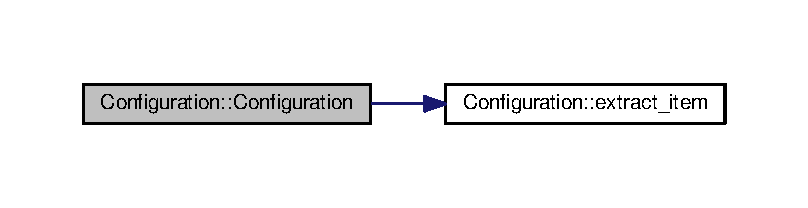
\includegraphics[width=350pt]{classConfiguration_a779947337bf652f0e773cb29f37f14ba_cgraph}
\end{center}
\end{figure}




\subsection{Member Function Documentation}
\hypertarget{classConfiguration_ac2ca184b014af7f7caa3ac487909a8f3}{\index{Configuration@{Configuration}!extract\-\_\-item@{extract\-\_\-item}}
\index{extract\-\_\-item@{extract\-\_\-item}!Configuration@{Configuration}}
\subsubsection[{extract\-\_\-item}]{\setlength{\rightskip}{0pt plus 5cm}char $\ast$ Configuration\-::extract\-\_\-item (
\begin{DoxyParamCaption}
\item[{char $\ast$const}]{string, }
\item[{char $\ast$const}]{left, }
\item[{const char $\ast$const}]{right}
\end{DoxyParamCaption}
)\hspace{0.3cm}{\ttfamily [private]}}}\label{classConfiguration_ac2ca184b014af7f7caa3ac487909a8f3}
This is an helper function used by Configuration\-File; it's used to parse input from configuration file. 

Here is the caller graph for this function\-:
\nopagebreak
\begin{figure}[H]
\begin{center}
\leavevmode
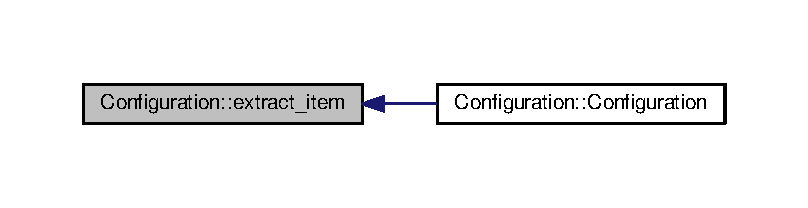
\includegraphics[width=350pt]{classConfiguration_ac2ca184b014af7f7caa3ac487909a8f3_icgraph}
\end{center}
\end{figure}


\hypertarget{classConfiguration_ad01eea5b98871f1cc4dbf28b9fe92093}{\index{Configuration@{Configuration}!operator\mbox{[}$\,$\mbox{]}@{operator[]}}
\index{operator\mbox{[}$\,$\mbox{]}@{operator[]}!Configuration@{Configuration}}
\subsubsection[{operator[]}]{\setlength{\rightskip}{0pt plus 5cm}std\-::string Configuration\-::operator\mbox{[}$\,$\mbox{]} (
\begin{DoxyParamCaption}
\item[{std\-::string}]{s}
\end{DoxyParamCaption}
)\hspace{0.3cm}{\ttfamily [inline]}}}\label{classConfiguration_ad01eea5b98871f1cc4dbf28b9fe92093}


\subsection{Member Data Documentation}
\hypertarget{classConfiguration_ab79bfcdc7339715a56a5a2f4a069bdda}{\index{Configuration@{Configuration}!configuration@{configuration}}
\index{configuration@{configuration}!Configuration@{Configuration}}
\subsubsection[{configuration}]{\setlength{\rightskip}{0pt plus 5cm}std\-::unordered\-\_\-map$<$std\-::string,std\-::string$>$ Configuration\-::configuration\hspace{0.3cm}{\ttfamily [private]}}}\label{classConfiguration_ab79bfcdc7339715a56a5a2f4a069bdda}
\hyperlink{classConfiguration}{Configuration} is a container which memorize data from the configuration file; it's an unordered map 

The documentation for this class was generated from the following files\-:\begin{DoxyCompactItemize}
\item 
/vagrant/\-P\-R\-O\-J\-E\-C\-T\-\_\-\-S\-P\-A\-R\-K/\-P\-A\-C\-S\-\_\-\-P\-R\-O\-J\-E\-C\-T/opt\-\_\-jr/src/\hyperlink{configuration_8hh}{configuration.\-hh}\item 
/vagrant/\-P\-R\-O\-J\-E\-C\-T\-\_\-\-S\-P\-A\-R\-K/\-P\-A\-C\-S\-\_\-\-P\-R\-O\-J\-E\-C\-T/opt\-\_\-jr/src/\hyperlink{configuration_8cpp}{configuration.\-cpp}\end{DoxyCompactItemize}

\hypertarget{classObjective__fun}{\section{Objective\-\_\-fun Class Reference}
\label{classObjective__fun}\index{Objective\-\_\-fun@{Objective\-\_\-fun}}
}


{\ttfamily \#include $<$objective\-\_\-fun.\-hh$>$}



Collaboration diagram for Objective\-\_\-fun\-:\nopagebreak
\begin{figure}[H]
\begin{center}
\leavevmode
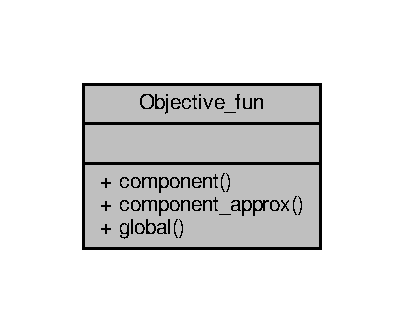
\includegraphics[width=194pt]{classObjective__fun__coll__graph}
\end{center}
\end{figure}
\subsection*{Public Member Functions}
\begin{DoxyCompactItemize}
\item 
double \hyperlink{classObjective__fun_a7d98b1f4e8a741fddc249e5134d5c3ef}{component} (\hyperlink{classConfiguration}{Configuration} \&configuration, M\-Y\-S\-Q\-L $\ast$conn, \hyperlink{classApplication}{Application} \&app, \hyperlink{classOpt__jr__parameters}{Opt\-\_\-jr\-\_\-parameters} \&par)
\item 
double \hyperlink{classObjective__fun_a551109cf9927773062e9e3668c00eb59}{component\-\_\-approx} (\hyperlink{classApplication}{Application} \&App, \hyperlink{classOpt__jr__parameters}{Opt\-\_\-jr\-\_\-parameters} \&par)
\item 
double \hyperlink{classObjective__fun_ae11b3facab75a7b7dc197d0a1a194d29}{global} (\hyperlink{classConfiguration}{Configuration} \&configuration, M\-Y\-S\-Q\-L $\ast$conn, \hyperlink{classBatch}{Batch} \&App\-\_\-manager, \hyperlink{classOpt__jr__parameters}{Opt\-\_\-jr\-\_\-parameters} \&par)
\end{DoxyCompactItemize}


\subsection{Detailed Description}
This class provides methods to evaluate the objective function in different ways. 

\subsection{Member Function Documentation}
\hypertarget{classObjective__fun_a7d98b1f4e8a741fddc249e5134d5c3ef}{\index{Objective\-\_\-fun@{Objective\-\_\-fun}!component@{component}}
\index{component@{component}!Objective_fun@{Objective\-\_\-fun}}
\subsubsection[{component}]{\setlength{\rightskip}{0pt plus 5cm}double Objective\-\_\-fun\-::component (
\begin{DoxyParamCaption}
\item[{{\bf Configuration} \&}]{configuration, }
\item[{M\-Y\-S\-Q\-L $\ast$}]{conn, }
\item[{{\bf Application} \&}]{app, }
\item[{{\bf Opt\-\_\-jr\-\_\-parameters} \&}]{par}
\end{DoxyParamCaption}
)}}\label{classObjective__fun_a7d98b1f4e8a741fddc249e5134d5c3ef}
component evaluates the contribution to the calculation of the objective function of one application. 

Here is the call graph for this function\-:
\nopagebreak
\begin{figure}[H]
\begin{center}
\leavevmode
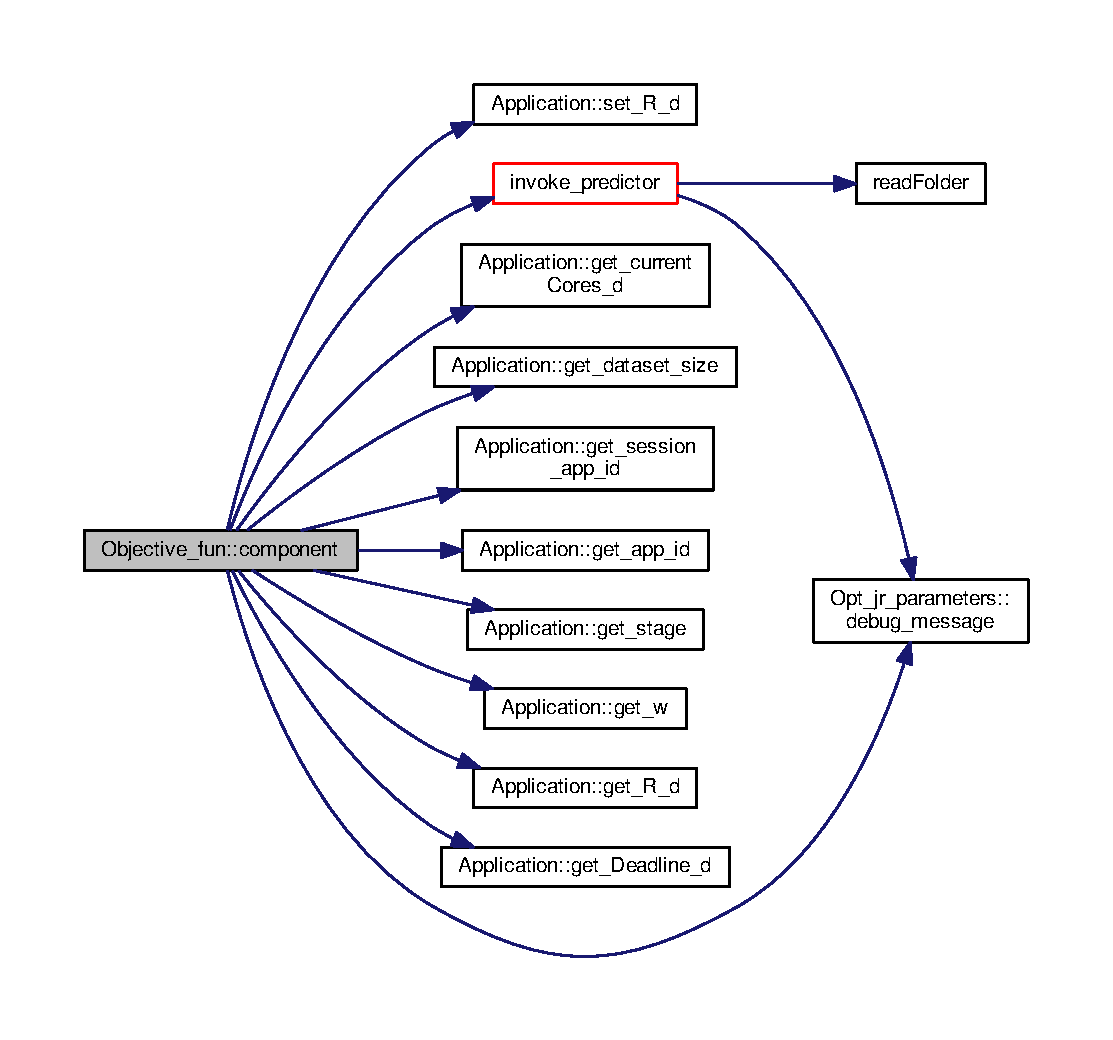
\includegraphics[width=350pt]{classObjective__fun_a7d98b1f4e8a741fddc249e5134d5c3ef_cgraph}
\end{center}
\end{figure}




Here is the caller graph for this function\-:
\nopagebreak
\begin{figure}[H]
\begin{center}
\leavevmode
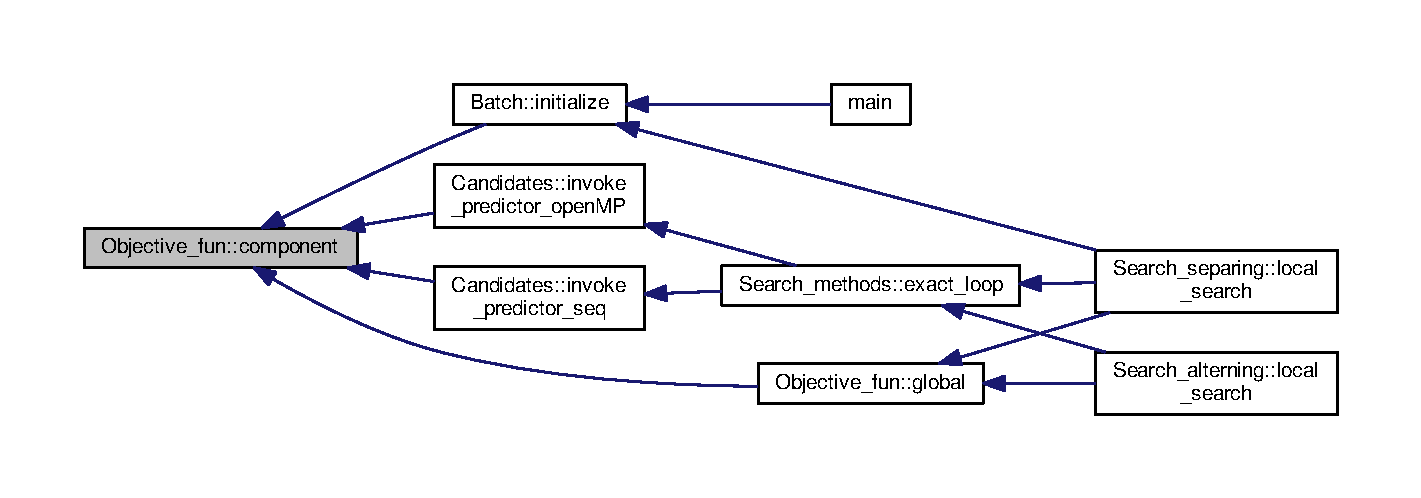
\includegraphics[width=350pt]{classObjective__fun_a7d98b1f4e8a741fddc249e5134d5c3ef_icgraph}
\end{center}
\end{figure}


\hypertarget{classObjective__fun_a551109cf9927773062e9e3668c00eb59}{\index{Objective\-\_\-fun@{Objective\-\_\-fun}!component\-\_\-approx@{component\-\_\-approx}}
\index{component\-\_\-approx@{component\-\_\-approx}!Objective_fun@{Objective\-\_\-fun}}
\subsubsection[{component\-\_\-approx}]{\setlength{\rightskip}{0pt plus 5cm}double Objective\-\_\-fun\-::component\-\_\-approx (
\begin{DoxyParamCaption}
\item[{{\bf Application} \&}]{App, }
\item[{{\bf Opt\-\_\-jr\-\_\-parameters} \&}]{par}
\end{DoxyParamCaption}
)}}\label{classObjective__fun_a551109cf9927773062e9e3668c00eb59}
component\-\_\-approx computes an approximation of the objective function (and update R\-\_\-d).

Name\-: component\-\_\-approx Output parameters\-: a double The value of the approximated objective function Description It computes an approximation of the objective function (and update R\-\_\-d) 

Here is the call graph for this function\-:
\nopagebreak
\begin{figure}[H]
\begin{center}
\leavevmode
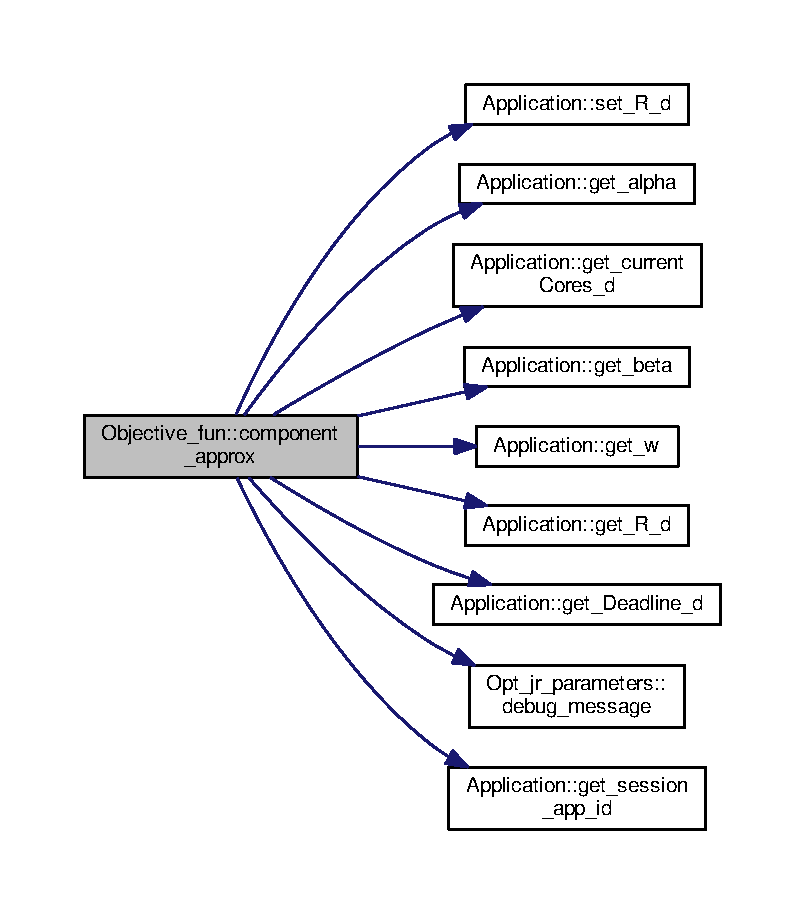
\includegraphics[width=350pt]{classObjective__fun_a551109cf9927773062e9e3668c00eb59_cgraph}
\end{center}
\end{figure}




Here is the caller graph for this function\-:
\nopagebreak
\begin{figure}[H]
\begin{center}
\leavevmode
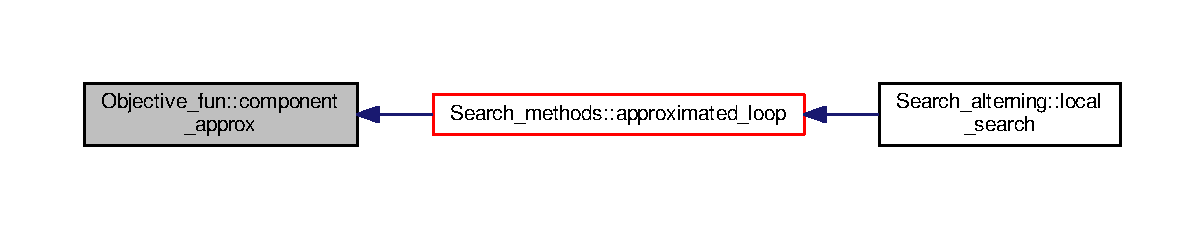
\includegraphics[width=350pt]{classObjective__fun_a551109cf9927773062e9e3668c00eb59_icgraph}
\end{center}
\end{figure}


\hypertarget{classObjective__fun_ae11b3facab75a7b7dc197d0a1a194d29}{\index{Objective\-\_\-fun@{Objective\-\_\-fun}!global@{global}}
\index{global@{global}!Objective_fun@{Objective\-\_\-fun}}
\subsubsection[{global}]{\setlength{\rightskip}{0pt plus 5cm}double Objective\-\_\-fun\-::global (
\begin{DoxyParamCaption}
\item[{{\bf Configuration} \&}]{configuration, }
\item[{M\-Y\-S\-Q\-L $\ast$}]{conn, }
\item[{{\bf Batch} \&}]{App\-\_\-manager, }
\item[{{\bf Opt\-\_\-jr\-\_\-parameters} \&}]{par}
\end{DoxyParamCaption}
)}}\label{classObjective__fun_ae11b3facab75a7b7dc197d0a1a194d29}
global computes the value of the total objective function. 

Here is the call graph for this function\-:
\nopagebreak
\begin{figure}[H]
\begin{center}
\leavevmode
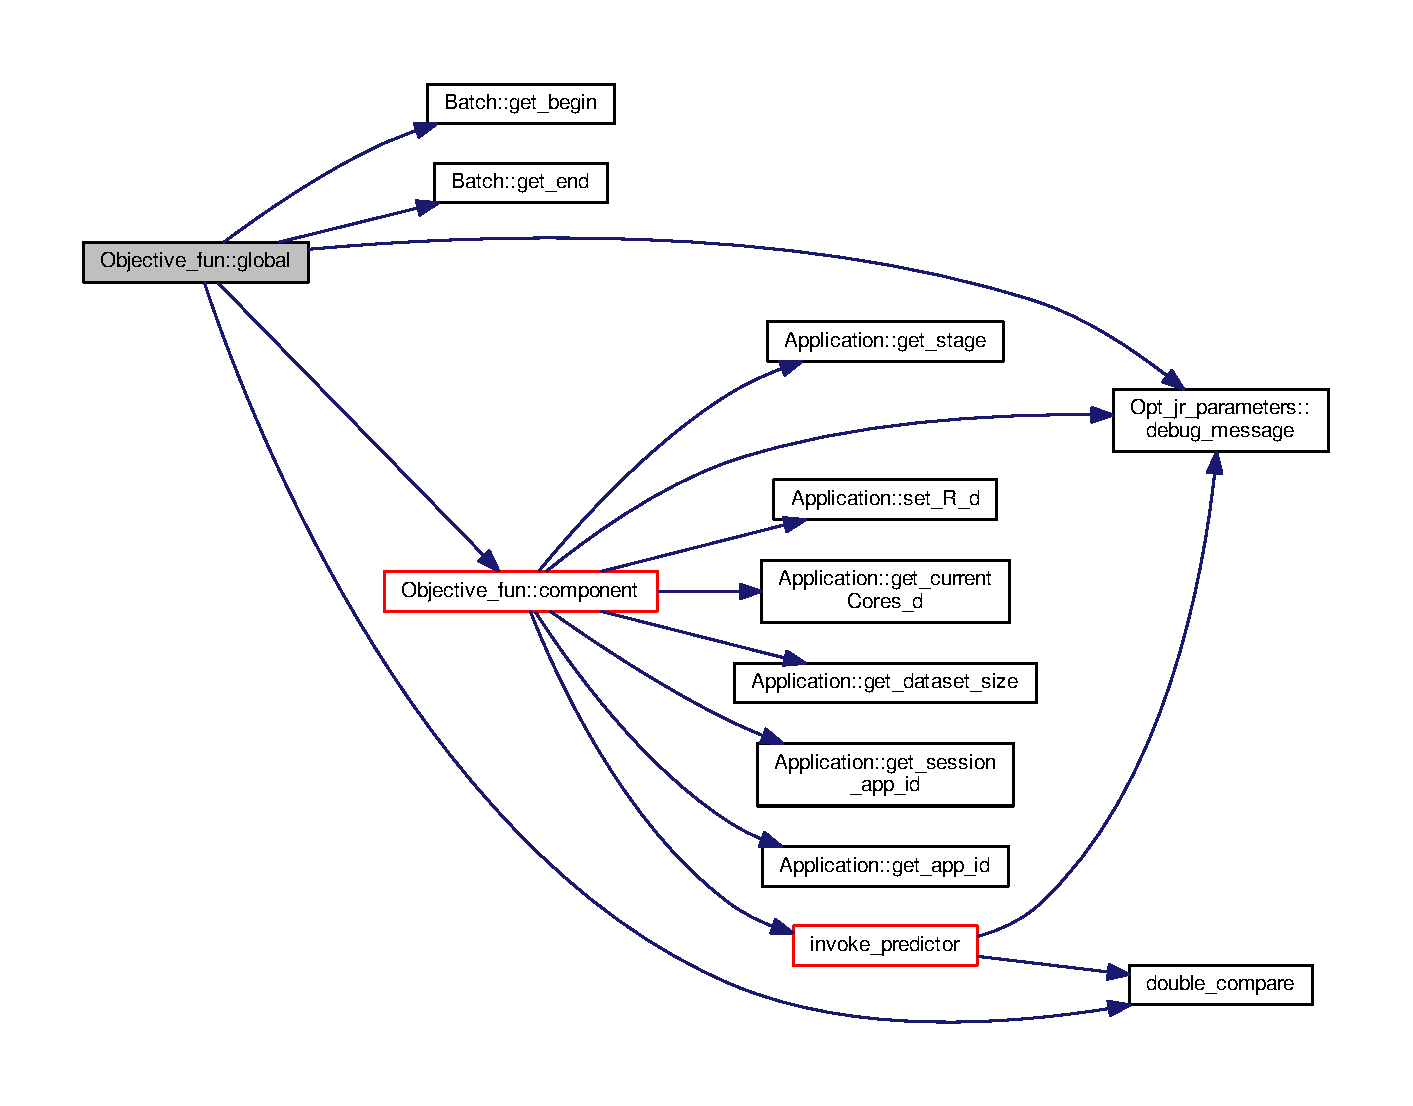
\includegraphics[width=350pt]{classObjective__fun_ae11b3facab75a7b7dc197d0a1a194d29_cgraph}
\end{center}
\end{figure}




Here is the caller graph for this function\-:\nopagebreak
\begin{figure}[H]
\begin{center}
\leavevmode
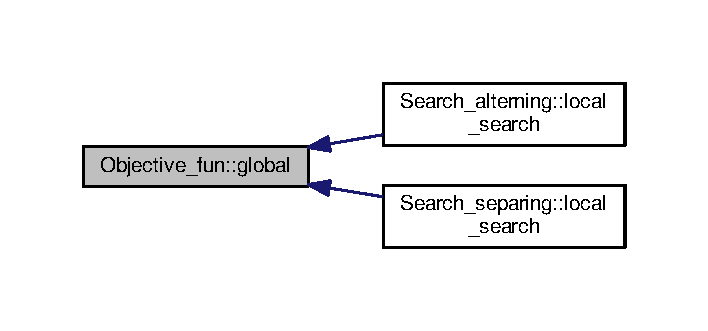
\includegraphics[width=340pt]{classObjective__fun_ae11b3facab75a7b7dc197d0a1a194d29_icgraph}
\end{center}
\end{figure}




The documentation for this class was generated from the following files\-:\begin{DoxyCompactItemize}
\item 
/vagrant/\-P\-R\-O\-J\-E\-C\-T\-\_\-\-S\-P\-A\-R\-K/\-P\-A\-C\-S\-\_\-\-P\-R\-O\-J\-E\-C\-T/opt\-\_\-jr/src/\hyperlink{objective__fun_8hh}{objective\-\_\-fun.\-hh}\item 
/vagrant/\-P\-R\-O\-J\-E\-C\-T\-\_\-\-S\-P\-A\-R\-K/\-P\-A\-C\-S\-\_\-\-P\-R\-O\-J\-E\-C\-T/opt\-\_\-jr/src/\hyperlink{objective__fun_8cpp}{objective\-\_\-fun.\-cpp}\end{DoxyCompactItemize}

\hypertarget{classOpt__jr__parameters}{\section{Opt\-\_\-jr\-\_\-parameters Class Reference}
\label{classOpt__jr__parameters}\index{Opt\-\_\-jr\-\_\-parameters@{Opt\-\_\-jr\-\_\-parameters}}
}


{\ttfamily \#include $<$opt\-\_\-jr\-\_\-parameters.\-hh$>$}



Collaboration diagram for Opt\-\_\-jr\-\_\-parameters\-:
\nopagebreak
\begin{figure}[H]
\begin{center}
\leavevmode
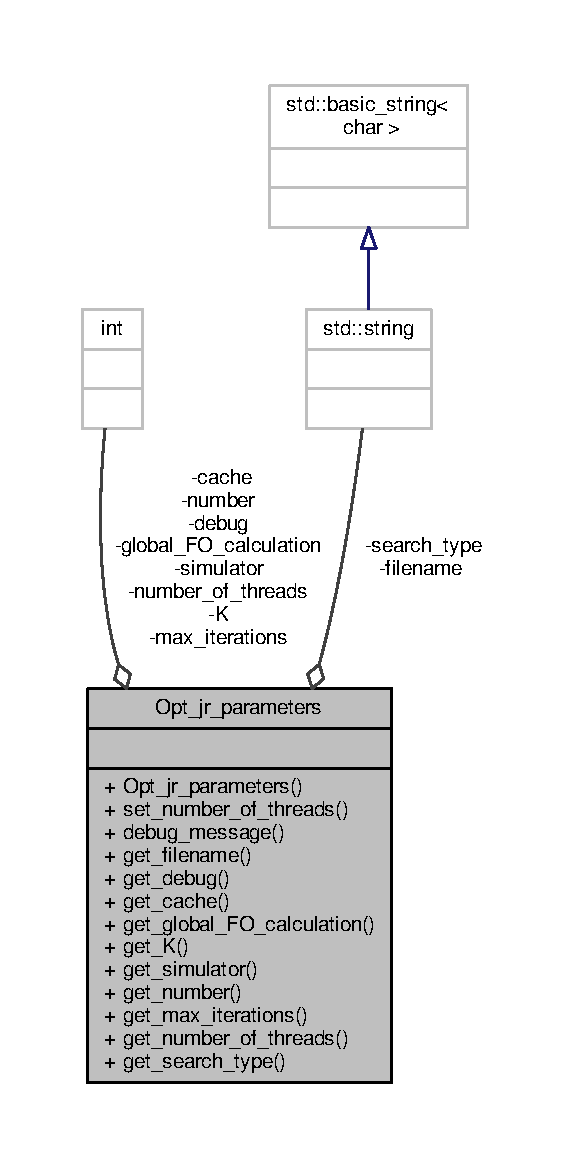
\includegraphics[width=272pt]{classOpt__jr__parameters__coll__graph}
\end{center}
\end{figure}
\subsection*{Public Member Functions}
\begin{DoxyCompactItemize}
\item 
\hyperlink{classOpt__jr__parameters_aae142f498b266523f275dba7a407326d}{Opt\-\_\-jr\-\_\-parameters} (char $\ast$$\ast$args, int argc)
\begin{DoxyCompactList}\small\item\em The constructor takes in input all the input from command line. \end{DoxyCompactList}\item 
void \hyperlink{classOpt__jr__parameters_a19769e398ca6969a851cc6584cfa4dd0}{set\-\_\-number\-\_\-of\-\_\-threads} (\hyperlink{classConfiguration}{Configuration} \&configuration)
\begin{DoxyCompactList}\small\item\em Set the number of threads\-: it looks in configuration file (0== \char`\"{}no parallelization\char`\"{}) \end{DoxyCompactList}\item 
void \hyperlink{classOpt__jr__parameters_a860bf209221b6c5e1c4394d1ae4a058f}{debug\-\_\-message} (std\-::string \&string)
\item 
const std\-::string \hyperlink{classOpt__jr__parameters_a7cef75cfec6d554805e311d7b4c37ef2}{get\-\_\-filename} ()
\item 
const int \hyperlink{classOpt__jr__parameters_ae22fb9f311cca37788ea5cf054e83aa7}{get\-\_\-debug} ()
\item 
const int \hyperlink{classOpt__jr__parameters_a38b9495684e078740fc009c7a25ef643}{get\-\_\-cache} ()
\item 
const int \hyperlink{classOpt__jr__parameters_a5437ef881f921ae81f5e3d93fbac7e2a}{get\-\_\-global\-\_\-\-F\-O\-\_\-calculation} ()
\item 
const int \hyperlink{classOpt__jr__parameters_a8b6c548de42e286a8848b198280aa2dc}{get\-\_\-\-K} ()
\item 
const int \hyperlink{classOpt__jr__parameters_a198ee52d6e6bd479255e57f3fe12af0b}{get\-\_\-simulator} ()
\item 
const int \hyperlink{classOpt__jr__parameters_a8bafd6844417b1f64ddefcf84fb726cb}{get\-\_\-number} ()
\item 
const int \hyperlink{classOpt__jr__parameters_a4666611fbf651a76876a0356ad204df1}{get\-\_\-max\-\_\-iterations} ()
\item 
const int \hyperlink{classOpt__jr__parameters_a186166286122c263aac7bb8fe56d6751}{get\-\_\-number\-\_\-of\-\_\-threads} ()
\item 
const std\-::string \hyperlink{classOpt__jr__parameters_a77f9d51e7183e9af98e6211f444ed6b4}{get\-\_\-search\-\_\-type} ()
\end{DoxyCompactItemize}
\subsection*{Private Attributes}
\begin{DoxyCompactItemize}
\item 
std\-::string \hyperlink{classOpt__jr__parameters_aae2da456acbf5ac035faec6e01015714}{filename}
\begin{DoxyCompactList}\small\item\em The csv file. \end{DoxyCompactList}\item 
int \hyperlink{classOpt__jr__parameters_ae8241c7d0f75864365575e4be23037a3}{debug}
\begin{DoxyCompactList}\small\item\em debug option\-: \char`\"{}y\char`\"{} prints every message, \char`\"{}n\char`\"{} only prints fatal errors \end{DoxyCompactList}\item 
int \hyperlink{classOpt__jr__parameters_ad4061078141fd36321c49fa9105e11a5}{cache}
\begin{DoxyCompactList}\small\item\em cache option\-: \char`\"{}y\char`\"{} makes use of the D\-B predictor cache table; \char`\"{}n\char`\"{} doesn't \end{DoxyCompactList}\item 
int \hyperlink{classOpt__jr__parameters_adf939a159428f604a0d524bee1234bf2}{global\-\_\-\-F\-O\-\_\-calculation}
\begin{DoxyCompactList}\small\item\em global F\-O calculation\-: \char`\"{}y\char`\"{} calculates at each loop of local\-Search function the global objective function value, \char`\"{}n\char`\"{} doesn't \end{DoxyCompactList}\item 
int \hyperlink{classOpt__jr__parameters_a71e4771571a4466646cd1433b038b8da}{K}
\begin{DoxyCompactList}\small\item\em Maximum depth\-: the search of candidates in the auxiliary list stops if this limit is exceeded. \end{DoxyCompactList}\item 
int \hyperlink{classOpt__jr__parameters_a032e1532dc68ecb39b2f2129c0d81449}{simulator}
\begin{DoxyCompactList}\small\item\em The simulator type\-: either dag\-Sim or Lundstrom. \end{DoxyCompactList}\item 
int \hyperlink{classOpt__jr__parameters_a3dfcb1783bcd6490733d10ced0833883}{number}
\begin{DoxyCompactList}\small\item\em Number of total cores available for the applications (N) \end{DoxyCompactList}\item 
int \hyperlink{classOpt__jr__parameters_aed595357c678f156b58e1010095b7efc}{max\-\_\-iterations}
\begin{DoxyCompactList}\small\item\em The maximum number of iterations in Local\-Search. \end{DoxyCompactList}\item 
int \hyperlink{classOpt__jr__parameters_a90838c460af325a8a453ffb7fad21eaa}{number\-\_\-of\-\_\-threads}
\begin{DoxyCompactList}\small\item\em The number of M\-P\-I threads. \end{DoxyCompactList}\item 
std\-::string \hyperlink{classOpt__jr__parameters_a0826424385c08cba6aff3c04e6eee423}{search\-\_\-type}
\begin{DoxyCompactList}\small\item\em type of localsearch to be used (alternating/separing) \end{DoxyCompactList}\end{DoxyCompactItemize}


\subsection{Detailed Description}
\hyperlink{classOpt__jr__parameters}{Opt\-\_\-jr\-\_\-parameters} saves parameters received from command line; once they are saved they are visible with public get\-\_\-$\ast$() functions 

\subsection{Constructor \& Destructor Documentation}
\hypertarget{classOpt__jr__parameters_aae142f498b266523f275dba7a407326d}{\index{Opt\-\_\-jr\-\_\-parameters@{Opt\-\_\-jr\-\_\-parameters}!Opt\-\_\-jr\-\_\-parameters@{Opt\-\_\-jr\-\_\-parameters}}
\index{Opt\-\_\-jr\-\_\-parameters@{Opt\-\_\-jr\-\_\-parameters}!Opt_jr_parameters@{Opt\-\_\-jr\-\_\-parameters}}
\subsubsection[{Opt\-\_\-jr\-\_\-parameters}]{\setlength{\rightskip}{0pt plus 5cm}Opt\-\_\-jr\-\_\-parameters\-::\-Opt\-\_\-jr\-\_\-parameters (
\begin{DoxyParamCaption}
\item[{char $\ast$$\ast$}]{args, }
\item[{int}]{argc}
\end{DoxyParamCaption}
)}}\label{classOpt__jr__parameters_aae142f498b266523f275dba7a407326d}


The constructor takes in input all the input from command line. 



Here is the call graph for this function\-:
\nopagebreak
\begin{figure}[H]
\begin{center}
\leavevmode
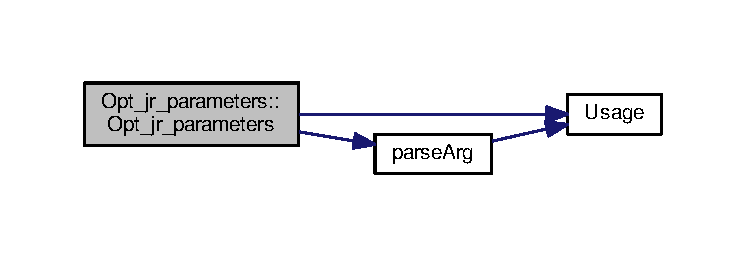
\includegraphics[width=350pt]{classOpt__jr__parameters_aae142f498b266523f275dba7a407326d_cgraph}
\end{center}
\end{figure}




\subsection{Member Function Documentation}
\hypertarget{classOpt__jr__parameters_a860bf209221b6c5e1c4394d1ae4a058f}{\index{Opt\-\_\-jr\-\_\-parameters@{Opt\-\_\-jr\-\_\-parameters}!debug\-\_\-message@{debug\-\_\-message}}
\index{debug\-\_\-message@{debug\-\_\-message}!Opt_jr_parameters@{Opt\-\_\-jr\-\_\-parameters}}
\subsubsection[{debug\-\_\-message}]{\setlength{\rightskip}{0pt plus 5cm}void Opt\-\_\-jr\-\_\-parameters\-::debug\-\_\-message (
\begin{DoxyParamCaption}
\item[{std\-::string \&}]{string}
\end{DoxyParamCaption}
)}}\label{classOpt__jr__parameters_a860bf209221b6c5e1c4394d1ae4a058f}
\hypertarget{classOpt__jr__parameters_a38b9495684e078740fc009c7a25ef643}{\index{Opt\-\_\-jr\-\_\-parameters@{Opt\-\_\-jr\-\_\-parameters}!get\-\_\-cache@{get\-\_\-cache}}
\index{get\-\_\-cache@{get\-\_\-cache}!Opt_jr_parameters@{Opt\-\_\-jr\-\_\-parameters}}
\subsubsection[{get\-\_\-cache}]{\setlength{\rightskip}{0pt plus 5cm}const int Opt\-\_\-jr\-\_\-parameters\-::get\-\_\-cache (
\begin{DoxyParamCaption}
{}
\end{DoxyParamCaption}
)\hspace{0.3cm}{\ttfamily [inline]}}}\label{classOpt__jr__parameters_a38b9495684e078740fc009c7a25ef643}


Here is the caller graph for this function\-:
\nopagebreak
\begin{figure}[H]
\begin{center}
\leavevmode
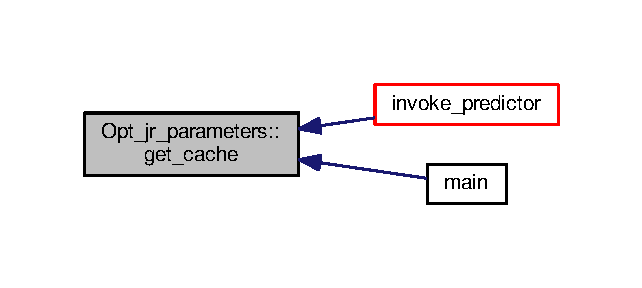
\includegraphics[width=308pt]{classOpt__jr__parameters_a38b9495684e078740fc009c7a25ef643_icgraph}
\end{center}
\end{figure}


\hypertarget{classOpt__jr__parameters_ae22fb9f311cca37788ea5cf054e83aa7}{\index{Opt\-\_\-jr\-\_\-parameters@{Opt\-\_\-jr\-\_\-parameters}!get\-\_\-debug@{get\-\_\-debug}}
\index{get\-\_\-debug@{get\-\_\-debug}!Opt_jr_parameters@{Opt\-\_\-jr\-\_\-parameters}}
\subsubsection[{get\-\_\-debug}]{\setlength{\rightskip}{0pt plus 5cm}const int Opt\-\_\-jr\-\_\-parameters\-::get\-\_\-debug (
\begin{DoxyParamCaption}
{}
\end{DoxyParamCaption}
)\hspace{0.3cm}{\ttfamily [inline]}}}\label{classOpt__jr__parameters_ae22fb9f311cca37788ea5cf054e83aa7}


Here is the caller graph for this function\-:
\nopagebreak
\begin{figure}[H]
\begin{center}
\leavevmode
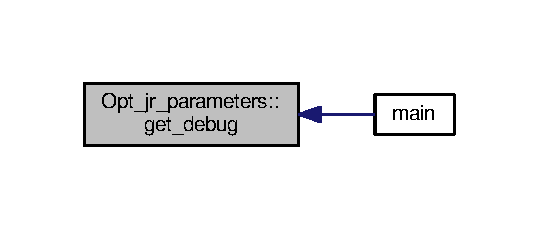
\includegraphics[width=258pt]{classOpt__jr__parameters_ae22fb9f311cca37788ea5cf054e83aa7_icgraph}
\end{center}
\end{figure}


\hypertarget{classOpt__jr__parameters_a7cef75cfec6d554805e311d7b4c37ef2}{\index{Opt\-\_\-jr\-\_\-parameters@{Opt\-\_\-jr\-\_\-parameters}!get\-\_\-filename@{get\-\_\-filename}}
\index{get\-\_\-filename@{get\-\_\-filename}!Opt_jr_parameters@{Opt\-\_\-jr\-\_\-parameters}}
\subsubsection[{get\-\_\-filename}]{\setlength{\rightskip}{0pt plus 5cm}const std\-::string Opt\-\_\-jr\-\_\-parameters\-::get\-\_\-filename (
\begin{DoxyParamCaption}
{}
\end{DoxyParamCaption}
)\hspace{0.3cm}{\ttfamily [inline]}}}\label{classOpt__jr__parameters_a7cef75cfec6d554805e311d7b4c37ef2}


Here is the caller graph for this function\-:
\nopagebreak
\begin{figure}[H]
\begin{center}
\leavevmode
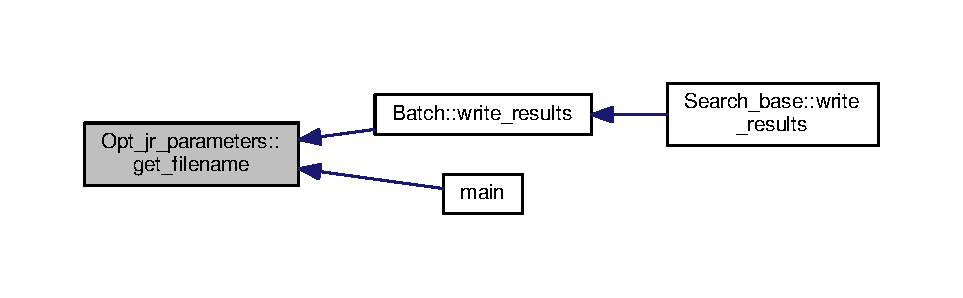
\includegraphics[width=324pt]{classOpt__jr__parameters_a7cef75cfec6d554805e311d7b4c37ef2_icgraph}
\end{center}
\end{figure}


\hypertarget{classOpt__jr__parameters_a5437ef881f921ae81f5e3d93fbac7e2a}{\index{Opt\-\_\-jr\-\_\-parameters@{Opt\-\_\-jr\-\_\-parameters}!get\-\_\-global\-\_\-\-F\-O\-\_\-calculation@{get\-\_\-global\-\_\-\-F\-O\-\_\-calculation}}
\index{get\-\_\-global\-\_\-\-F\-O\-\_\-calculation@{get\-\_\-global\-\_\-\-F\-O\-\_\-calculation}!Opt_jr_parameters@{Opt\-\_\-jr\-\_\-parameters}}
\subsubsection[{get\-\_\-global\-\_\-\-F\-O\-\_\-calculation}]{\setlength{\rightskip}{0pt plus 5cm}const int Opt\-\_\-jr\-\_\-parameters\-::get\-\_\-global\-\_\-\-F\-O\-\_\-calculation (
\begin{DoxyParamCaption}
{}
\end{DoxyParamCaption}
)\hspace{0.3cm}{\ttfamily [inline]}}}\label{classOpt__jr__parameters_a5437ef881f921ae81f5e3d93fbac7e2a}
\hypertarget{classOpt__jr__parameters_a8b6c548de42e286a8848b198280aa2dc}{\index{Opt\-\_\-jr\-\_\-parameters@{Opt\-\_\-jr\-\_\-parameters}!get\-\_\-\-K@{get\-\_\-\-K}}
\index{get\-\_\-\-K@{get\-\_\-\-K}!Opt_jr_parameters@{Opt\-\_\-jr\-\_\-parameters}}
\subsubsection[{get\-\_\-\-K}]{\setlength{\rightskip}{0pt plus 5cm}const int Opt\-\_\-jr\-\_\-parameters\-::get\-\_\-\-K (
\begin{DoxyParamCaption}
{}
\end{DoxyParamCaption}
)\hspace{0.3cm}{\ttfamily [inline]}}}\label{classOpt__jr__parameters_a8b6c548de42e286a8848b198280aa2dc}
\hypertarget{classOpt__jr__parameters_a4666611fbf651a76876a0356ad204df1}{\index{Opt\-\_\-jr\-\_\-parameters@{Opt\-\_\-jr\-\_\-parameters}!get\-\_\-max\-\_\-iterations@{get\-\_\-max\-\_\-iterations}}
\index{get\-\_\-max\-\_\-iterations@{get\-\_\-max\-\_\-iterations}!Opt_jr_parameters@{Opt\-\_\-jr\-\_\-parameters}}
\subsubsection[{get\-\_\-max\-\_\-iterations}]{\setlength{\rightskip}{0pt plus 5cm}const int Opt\-\_\-jr\-\_\-parameters\-::get\-\_\-max\-\_\-iterations (
\begin{DoxyParamCaption}
{}
\end{DoxyParamCaption}
)\hspace{0.3cm}{\ttfamily [inline]}}}\label{classOpt__jr__parameters_a4666611fbf651a76876a0356ad204df1}
\hypertarget{classOpt__jr__parameters_a8bafd6844417b1f64ddefcf84fb726cb}{\index{Opt\-\_\-jr\-\_\-parameters@{Opt\-\_\-jr\-\_\-parameters}!get\-\_\-number@{get\-\_\-number}}
\index{get\-\_\-number@{get\-\_\-number}!Opt_jr_parameters@{Opt\-\_\-jr\-\_\-parameters}}
\subsubsection[{get\-\_\-number}]{\setlength{\rightskip}{0pt plus 5cm}const int Opt\-\_\-jr\-\_\-parameters\-::get\-\_\-number (
\begin{DoxyParamCaption}
{}
\end{DoxyParamCaption}
)\hspace{0.3cm}{\ttfamily [inline]}}}\label{classOpt__jr__parameters_a8bafd6844417b1f64ddefcf84fb726cb}
\hypertarget{classOpt__jr__parameters_a186166286122c263aac7bb8fe56d6751}{\index{Opt\-\_\-jr\-\_\-parameters@{Opt\-\_\-jr\-\_\-parameters}!get\-\_\-number\-\_\-of\-\_\-threads@{get\-\_\-number\-\_\-of\-\_\-threads}}
\index{get\-\_\-number\-\_\-of\-\_\-threads@{get\-\_\-number\-\_\-of\-\_\-threads}!Opt_jr_parameters@{Opt\-\_\-jr\-\_\-parameters}}
\subsubsection[{get\-\_\-number\-\_\-of\-\_\-threads}]{\setlength{\rightskip}{0pt plus 5cm}const int Opt\-\_\-jr\-\_\-parameters\-::get\-\_\-number\-\_\-of\-\_\-threads (
\begin{DoxyParamCaption}
{}
\end{DoxyParamCaption}
)\hspace{0.3cm}{\ttfamily [inline]}}}\label{classOpt__jr__parameters_a186166286122c263aac7bb8fe56d6751}
\hypertarget{classOpt__jr__parameters_a77f9d51e7183e9af98e6211f444ed6b4}{\index{Opt\-\_\-jr\-\_\-parameters@{Opt\-\_\-jr\-\_\-parameters}!get\-\_\-search\-\_\-type@{get\-\_\-search\-\_\-type}}
\index{get\-\_\-search\-\_\-type@{get\-\_\-search\-\_\-type}!Opt_jr_parameters@{Opt\-\_\-jr\-\_\-parameters}}
\subsubsection[{get\-\_\-search\-\_\-type}]{\setlength{\rightskip}{0pt plus 5cm}const std\-::string Opt\-\_\-jr\-\_\-parameters\-::get\-\_\-search\-\_\-type (
\begin{DoxyParamCaption}
{}
\end{DoxyParamCaption}
)\hspace{0.3cm}{\ttfamily [inline]}}}\label{classOpt__jr__parameters_a77f9d51e7183e9af98e6211f444ed6b4}


Here is the caller graph for this function\-:
\nopagebreak
\begin{figure}[H]
\begin{center}
\leavevmode
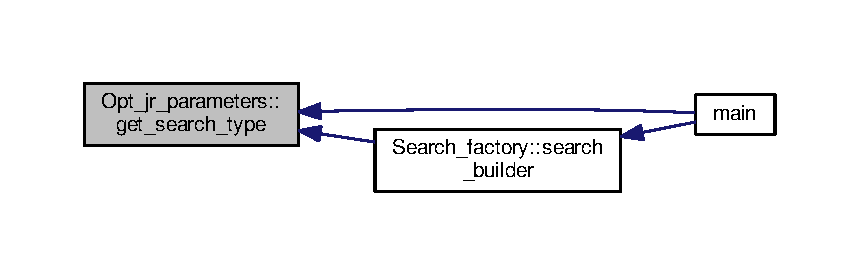
\includegraphics[width=350pt]{classOpt__jr__parameters_a77f9d51e7183e9af98e6211f444ed6b4_icgraph}
\end{center}
\end{figure}


\hypertarget{classOpt__jr__parameters_a198ee52d6e6bd479255e57f3fe12af0b}{\index{Opt\-\_\-jr\-\_\-parameters@{Opt\-\_\-jr\-\_\-parameters}!get\-\_\-simulator@{get\-\_\-simulator}}
\index{get\-\_\-simulator@{get\-\_\-simulator}!Opt_jr_parameters@{Opt\-\_\-jr\-\_\-parameters}}
\subsubsection[{get\-\_\-simulator}]{\setlength{\rightskip}{0pt plus 5cm}const int Opt\-\_\-jr\-\_\-parameters\-::get\-\_\-simulator (
\begin{DoxyParamCaption}
{}
\end{DoxyParamCaption}
)\hspace{0.3cm}{\ttfamily [inline]}}}\label{classOpt__jr__parameters_a198ee52d6e6bd479255e57f3fe12af0b}


Here is the caller graph for this function\-:
\nopagebreak
\begin{figure}[H]
\begin{center}
\leavevmode
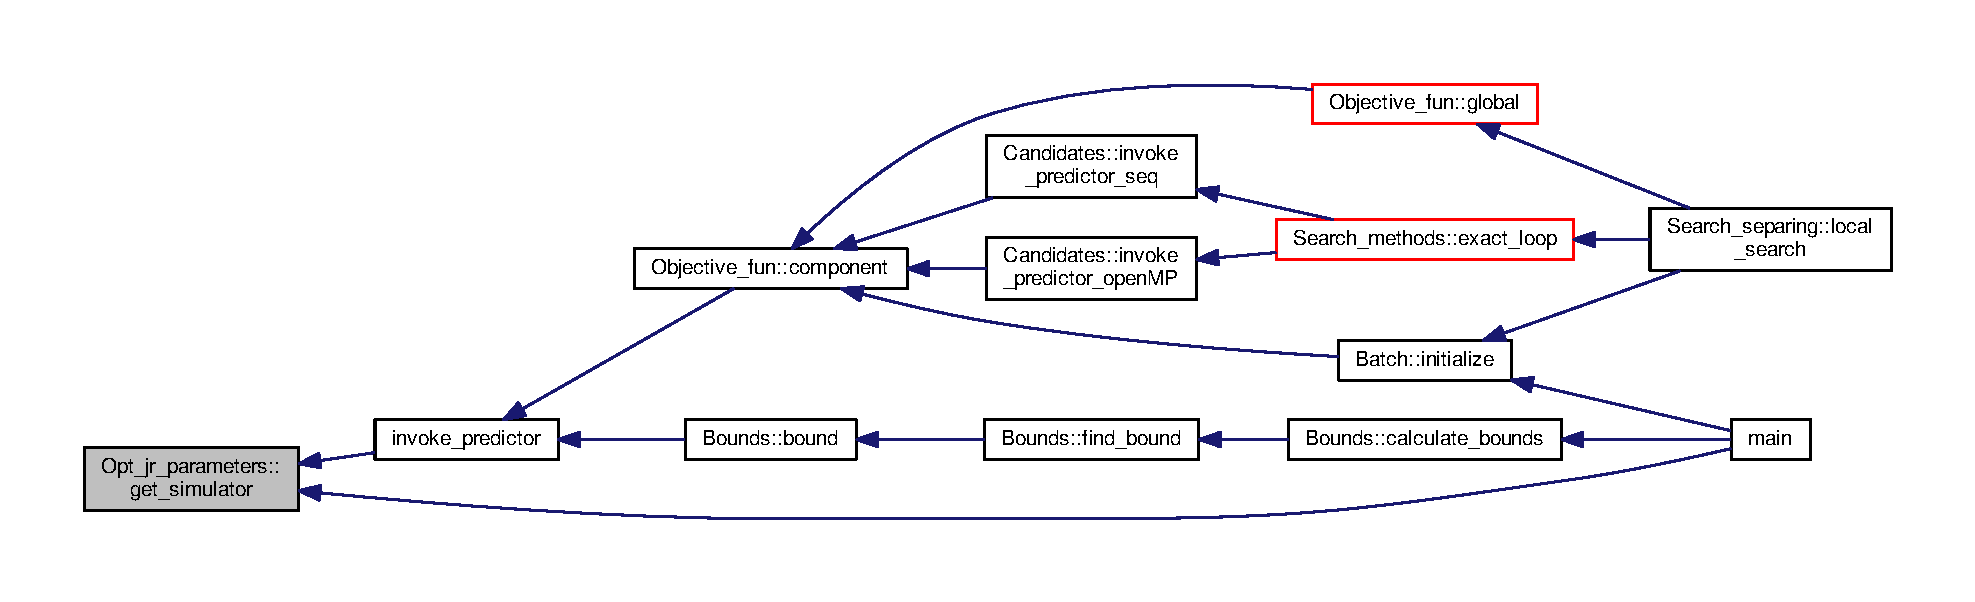
\includegraphics[width=308pt]{classOpt__jr__parameters_a198ee52d6e6bd479255e57f3fe12af0b_icgraph}
\end{center}
\end{figure}


\hypertarget{classOpt__jr__parameters_a19769e398ca6969a851cc6584cfa4dd0}{\index{Opt\-\_\-jr\-\_\-parameters@{Opt\-\_\-jr\-\_\-parameters}!set\-\_\-number\-\_\-of\-\_\-threads@{set\-\_\-number\-\_\-of\-\_\-threads}}
\index{set\-\_\-number\-\_\-of\-\_\-threads@{set\-\_\-number\-\_\-of\-\_\-threads}!Opt_jr_parameters@{Opt\-\_\-jr\-\_\-parameters}}
\subsubsection[{set\-\_\-number\-\_\-of\-\_\-threads}]{\setlength{\rightskip}{0pt plus 5cm}void Opt\-\_\-jr\-\_\-parameters\-::set\-\_\-number\-\_\-of\-\_\-threads (
\begin{DoxyParamCaption}
\item[{{\bf Configuration} \&}]{configuration}
\end{DoxyParamCaption}
)}}\label{classOpt__jr__parameters_a19769e398ca6969a851cc6584cfa4dd0}


Set the number of threads\-: it looks in configuration file (0== \char`\"{}no parallelization\char`\"{}) 



Here is the caller graph for this function\-:
\nopagebreak
\begin{figure}[H]
\begin{center}
\leavevmode
\includegraphics[width=274pt]{classOpt__jr__parameters_a19769e398ca6969a851cc6584cfa4dd0_icgraph}
\end{center}
\end{figure}




\subsection{Member Data Documentation}
\hypertarget{classOpt__jr__parameters_ad4061078141fd36321c49fa9105e11a5}{\index{Opt\-\_\-jr\-\_\-parameters@{Opt\-\_\-jr\-\_\-parameters}!cache@{cache}}
\index{cache@{cache}!Opt_jr_parameters@{Opt\-\_\-jr\-\_\-parameters}}
\subsubsection[{cache}]{\setlength{\rightskip}{0pt plus 5cm}int Opt\-\_\-jr\-\_\-parameters\-::cache\hspace{0.3cm}{\ttfamily [private]}}}\label{classOpt__jr__parameters_ad4061078141fd36321c49fa9105e11a5}


cache option\-: \char`\"{}y\char`\"{} makes use of the D\-B predictor cache table; \char`\"{}n\char`\"{} doesn't 

\hypertarget{classOpt__jr__parameters_ae8241c7d0f75864365575e4be23037a3}{\index{Opt\-\_\-jr\-\_\-parameters@{Opt\-\_\-jr\-\_\-parameters}!debug@{debug}}
\index{debug@{debug}!Opt_jr_parameters@{Opt\-\_\-jr\-\_\-parameters}}
\subsubsection[{debug}]{\setlength{\rightskip}{0pt plus 5cm}int Opt\-\_\-jr\-\_\-parameters\-::debug\hspace{0.3cm}{\ttfamily [private]}}}\label{classOpt__jr__parameters_ae8241c7d0f75864365575e4be23037a3}


debug option\-: \char`\"{}y\char`\"{} prints every message, \char`\"{}n\char`\"{} only prints fatal errors 

\hypertarget{classOpt__jr__parameters_aae2da456acbf5ac035faec6e01015714}{\index{Opt\-\_\-jr\-\_\-parameters@{Opt\-\_\-jr\-\_\-parameters}!filename@{filename}}
\index{filename@{filename}!Opt_jr_parameters@{Opt\-\_\-jr\-\_\-parameters}}
\subsubsection[{filename}]{\setlength{\rightskip}{0pt plus 5cm}std\-::string Opt\-\_\-jr\-\_\-parameters\-::filename\hspace{0.3cm}{\ttfamily [private]}}}\label{classOpt__jr__parameters_aae2da456acbf5ac035faec6e01015714}


The csv file. 

\hypertarget{classOpt__jr__parameters_adf939a159428f604a0d524bee1234bf2}{\index{Opt\-\_\-jr\-\_\-parameters@{Opt\-\_\-jr\-\_\-parameters}!global\-\_\-\-F\-O\-\_\-calculation@{global\-\_\-\-F\-O\-\_\-calculation}}
\index{global\-\_\-\-F\-O\-\_\-calculation@{global\-\_\-\-F\-O\-\_\-calculation}!Opt_jr_parameters@{Opt\-\_\-jr\-\_\-parameters}}
\subsubsection[{global\-\_\-\-F\-O\-\_\-calculation}]{\setlength{\rightskip}{0pt plus 5cm}int Opt\-\_\-jr\-\_\-parameters\-::global\-\_\-\-F\-O\-\_\-calculation\hspace{0.3cm}{\ttfamily [private]}}}\label{classOpt__jr__parameters_adf939a159428f604a0d524bee1234bf2}


global F\-O calculation\-: \char`\"{}y\char`\"{} calculates at each loop of local\-Search function the global objective function value, \char`\"{}n\char`\"{} doesn't 

\hypertarget{classOpt__jr__parameters_a71e4771571a4466646cd1433b038b8da}{\index{Opt\-\_\-jr\-\_\-parameters@{Opt\-\_\-jr\-\_\-parameters}!K@{K}}
\index{K@{K}!Opt_jr_parameters@{Opt\-\_\-jr\-\_\-parameters}}
\subsubsection[{K}]{\setlength{\rightskip}{0pt plus 5cm}int Opt\-\_\-jr\-\_\-parameters\-::\-K\hspace{0.3cm}{\ttfamily [private]}}}\label{classOpt__jr__parameters_a71e4771571a4466646cd1433b038b8da}


Maximum depth\-: the search of candidates in the auxiliary list stops if this limit is exceeded. 

\hypertarget{classOpt__jr__parameters_aed595357c678f156b58e1010095b7efc}{\index{Opt\-\_\-jr\-\_\-parameters@{Opt\-\_\-jr\-\_\-parameters}!max\-\_\-iterations@{max\-\_\-iterations}}
\index{max\-\_\-iterations@{max\-\_\-iterations}!Opt_jr_parameters@{Opt\-\_\-jr\-\_\-parameters}}
\subsubsection[{max\-\_\-iterations}]{\setlength{\rightskip}{0pt plus 5cm}int Opt\-\_\-jr\-\_\-parameters\-::max\-\_\-iterations\hspace{0.3cm}{\ttfamily [private]}}}\label{classOpt__jr__parameters_aed595357c678f156b58e1010095b7efc}


The maximum number of iterations in Local\-Search. 

\hypertarget{classOpt__jr__parameters_a3dfcb1783bcd6490733d10ced0833883}{\index{Opt\-\_\-jr\-\_\-parameters@{Opt\-\_\-jr\-\_\-parameters}!number@{number}}
\index{number@{number}!Opt_jr_parameters@{Opt\-\_\-jr\-\_\-parameters}}
\subsubsection[{number}]{\setlength{\rightskip}{0pt plus 5cm}int Opt\-\_\-jr\-\_\-parameters\-::number\hspace{0.3cm}{\ttfamily [private]}}}\label{classOpt__jr__parameters_a3dfcb1783bcd6490733d10ced0833883}


Number of total cores available for the applications (N) 

\hypertarget{classOpt__jr__parameters_a90838c460af325a8a453ffb7fad21eaa}{\index{Opt\-\_\-jr\-\_\-parameters@{Opt\-\_\-jr\-\_\-parameters}!number\-\_\-of\-\_\-threads@{number\-\_\-of\-\_\-threads}}
\index{number\-\_\-of\-\_\-threads@{number\-\_\-of\-\_\-threads}!Opt_jr_parameters@{Opt\-\_\-jr\-\_\-parameters}}
\subsubsection[{number\-\_\-of\-\_\-threads}]{\setlength{\rightskip}{0pt plus 5cm}int Opt\-\_\-jr\-\_\-parameters\-::number\-\_\-of\-\_\-threads\hspace{0.3cm}{\ttfamily [private]}}}\label{classOpt__jr__parameters_a90838c460af325a8a453ffb7fad21eaa}


The number of M\-P\-I threads. 

\hypertarget{classOpt__jr__parameters_a0826424385c08cba6aff3c04e6eee423}{\index{Opt\-\_\-jr\-\_\-parameters@{Opt\-\_\-jr\-\_\-parameters}!search\-\_\-type@{search\-\_\-type}}
\index{search\-\_\-type@{search\-\_\-type}!Opt_jr_parameters@{Opt\-\_\-jr\-\_\-parameters}}
\subsubsection[{search\-\_\-type}]{\setlength{\rightskip}{0pt plus 5cm}std\-::string Opt\-\_\-jr\-\_\-parameters\-::search\-\_\-type\hspace{0.3cm}{\ttfamily [private]}}}\label{classOpt__jr__parameters_a0826424385c08cba6aff3c04e6eee423}


type of localsearch to be used (alternating/separing) 

\hypertarget{classOpt__jr__parameters_a032e1532dc68ecb39b2f2129c0d81449}{\index{Opt\-\_\-jr\-\_\-parameters@{Opt\-\_\-jr\-\_\-parameters}!simulator@{simulator}}
\index{simulator@{simulator}!Opt_jr_parameters@{Opt\-\_\-jr\-\_\-parameters}}
\subsubsection[{simulator}]{\setlength{\rightskip}{0pt plus 5cm}int Opt\-\_\-jr\-\_\-parameters\-::simulator\hspace{0.3cm}{\ttfamily [private]}}}\label{classOpt__jr__parameters_a032e1532dc68ecb39b2f2129c0d81449}


The simulator type\-: either dag\-Sim or Lundstrom. 



The documentation for this class was generated from the following files\-:\begin{DoxyCompactItemize}
\item 
/vagrant/\-P\-R\-O\-J\-E\-C\-T\-\_\-\-S\-P\-A\-R\-K/\-P\-A\-C\-S\-\_\-\-P\-R\-O\-J\-E\-C\-T/opt\-\_\-jr/src/\hyperlink{opt__jr__parameters_8hh}{opt\-\_\-jr\-\_\-parameters.\-hh}\item 
/vagrant/\-P\-R\-O\-J\-E\-C\-T\-\_\-\-S\-P\-A\-R\-K/\-P\-A\-C\-S\-\_\-\-P\-R\-O\-J\-E\-C\-T/opt\-\_\-jr/src/\hyperlink{opt__jr__parameters_8cpp}{opt\-\_\-jr\-\_\-parameters.\-cpp}\end{DoxyCompactItemize}

\hypertarget{classSearch}{\section{Search$<$ Policy $>$ Class Template Reference}
\label{classSearch}\index{Search$<$ Policy $>$@{Search$<$ Policy $>$}}
}


{\ttfamily \#include $<$search.\-hh$>$}



Inheritance diagram for Search$<$ Policy $>$\-:
\nopagebreak
\begin{figure}[H]
\begin{center}
\leavevmode
\includegraphics[width=188pt]{classSearch__inherit__graph}
\end{center}
\end{figure}


Collaboration diagram for Search$<$ Policy $>$\-:
\nopagebreak
\begin{figure}[H]
\begin{center}
\leavevmode
\includegraphics[width=213pt]{classSearch__coll__graph}
\end{center}
\end{figure}
\subsection*{Public Member Functions}
\begin{DoxyCompactItemize}
\item 
\hyperlink{classSearch_a59b826749138fdaa93c41b1e0697da58}{Search} (\hyperlink{classBatch}{Batch} app\-\_\-m)
\item 
void \hyperlink{classSearch_a32d434fae76c18149f8b15aedadc5f75}{local\-\_\-search} (\hyperlink{classConfiguration}{Configuration} \&configuration, M\-Y\-S\-Q\-L $\ast$conn, \hyperlink{classOpt__jr__parameters}{Opt\-\_\-jr\-\_\-parameters} \&par)
\end{DoxyCompactItemize}
\subsection*{Additional Inherited Members}


\subsection{Detailed Description}
\subsubsection*{template$<$class Policy$>$class Search$<$ Policy $>$}

T\-O\-D\-O\-: modify descript. \char`\"{}\-Search\char`\"{} class provides methods to find a solution minimizing the objective function. Actually only one method is supported. 

\subsection{Constructor \& Destructor Documentation}
\hypertarget{classSearch_a59b826749138fdaa93c41b1e0697da58}{\index{Search@{Search}!Search@{Search}}
\index{Search@{Search}!Search@{Search}}
\subsubsection[{Search}]{\setlength{\rightskip}{0pt plus 5cm}template$<$class Policy $>$ {\bf Search}$<$ Policy $>$\-::{\bf Search} (
\begin{DoxyParamCaption}
\item[{{\bf Batch}}]{app\-\_\-m}
\end{DoxyParamCaption}
)\hspace{0.3cm}{\ttfamily [inline]}}}\label{classSearch_a59b826749138fdaa93c41b1e0697da58}


\subsection{Member Function Documentation}
\hypertarget{classSearch_a32d434fae76c18149f8b15aedadc5f75}{\index{Search@{Search}!local\-\_\-search@{local\-\_\-search}}
\index{local\-\_\-search@{local\-\_\-search}!Search@{Search}}
\subsubsection[{local\-\_\-search}]{\setlength{\rightskip}{0pt plus 5cm}template$<$class Policy $>$ void {\bf Search}$<$ Policy $>$\-::local\-\_\-search (
\begin{DoxyParamCaption}
\item[{{\bf Configuration} \&}]{configuration, }
\item[{M\-Y\-S\-Q\-L $\ast$}]{conn, }
\item[{{\bf Opt\-\_\-jr\-\_\-parameters} \&}]{par}
\end{DoxyParamCaption}
)\hspace{0.3cm}{\ttfamily [inline]}, {\ttfamily [virtual]}}}\label{classSearch_a32d434fae76c18149f8b15aedadc5f75}
local\-\_\-search perform a local search of a solution minimizing the objective function; it performs cores exchanges between pairs of application and chooses the best pair. The search stops when no improvements are possible or the maximum number of iteration is reached. The function looks before at approximated values of objective function and then for the potential best pairs it invokes the predictor. 

Implements \hyperlink{classSearch__base_ab3730b1118efbe97065f1ea9715a90dc}{Search\-\_\-base}.



The documentation for this class was generated from the following file\-:\begin{DoxyCompactItemize}
\item 
/vagrant/\-P\-R\-O\-J\-E\-C\-T\-\_\-\-S\-P\-A\-R\-K/\-P\-A\-C\-S\-\_\-\-P\-R\-O\-J\-E\-C\-T/opt\-\_\-jr/src/\hyperlink{search_8hh}{search.\-hh}\end{DoxyCompactItemize}

\hypertarget{classSearch__alterning}{\section{Search\-\_\-alterning Class Reference}
\label{classSearch__alterning}\index{Search\-\_\-alterning@{Search\-\_\-alterning}}
}


{\ttfamily \#include $<$search\-\_\-alterning.\-hh$>$}



Inheritance diagram for Search\-\_\-alterning\-:\nopagebreak
\begin{figure}[H]
\begin{center}
\leavevmode
\includegraphics[width=192pt]{classSearch__alterning__inherit__graph}
\end{center}
\end{figure}


Collaboration diagram for Search\-\_\-alterning\-:\nopagebreak
\begin{figure}[H]
\begin{center}
\leavevmode
\includegraphics[width=192pt]{classSearch__alterning__coll__graph}
\end{center}
\end{figure}
\subsection*{Public Member Functions}
\begin{DoxyCompactItemize}
\item 
void \hyperlink{classSearch__alterning_a981af51221c3749c4c20e58b8a622cb1}{local\-\_\-search} (\hyperlink{classBatch}{Batch} \&app\-\_\-manager, \hyperlink{classConfiguration}{Configuration} \&configuration, M\-Y\-S\-Q\-L $\ast$conn, \hyperlink{classOpt__jr__parameters}{Opt\-\_\-jr\-\_\-parameters} \&par)
\end{DoxyCompactItemize}


\subsection{Detailed Description}
\hyperlink{classSearch__alterning}{Search\-\_\-alterning} is a policy-\/class\-: it's passed as a template argument to \hyperlink{classSearch}{Search} in order to set the local\-\_\-search method. The local\-\_\-search methods performs a single loop in which at each iteration an approximated value for the objective function is evaluated for each move and then the objective function is evaluated for most profitable moves. 

\subsection{Member Function Documentation}
\hypertarget{classSearch__alterning_a981af51221c3749c4c20e58b8a622cb1}{\index{Search\-\_\-alterning@{Search\-\_\-alterning}!local\-\_\-search@{local\-\_\-search}}
\index{local\-\_\-search@{local\-\_\-search}!Search_alterning@{Search\-\_\-alterning}}
\subsubsection[{local\-\_\-search}]{\setlength{\rightskip}{0pt plus 5cm}void Search\-\_\-alterning\-::local\-\_\-search (
\begin{DoxyParamCaption}
\item[{{\bf Batch} \&}]{app\-\_\-manager, }
\item[{{\bf Configuration} \&}]{configuration, }
\item[{M\-Y\-S\-Q\-L $\ast$}]{conn, }
\item[{{\bf Opt\-\_\-jr\-\_\-parameters} \&}]{par}
\end{DoxyParamCaption}
)}}\label{classSearch__alterning_a981af51221c3749c4c20e58b8a622cb1}
The local\-\_\-search methods performs a single loop in which at each iteration an approximated value for the objective function is evaluated for each move and then the objective function is evaluated for most profitable moves. 

Here is the call graph for this function\-:
\nopagebreak
\begin{figure}[H]
\begin{center}
\leavevmode
\includegraphics[width=350pt]{classSearch__alterning_a981af51221c3749c4c20e58b8a622cb1_cgraph}
\end{center}
\end{figure}




The documentation for this class was generated from the following files\-:\begin{DoxyCompactItemize}
\item 
/vagrant/\-P\-R\-O\-J\-E\-C\-T\-\_\-\-S\-P\-A\-R\-K/\-P\-A\-C\-S\-\_\-\-P\-R\-O\-J\-E\-C\-T/opt\-\_\-jr/src/\hyperlink{search__alterning_8hh}{search\-\_\-alterning.\-hh}\item 
/vagrant/\-P\-R\-O\-J\-E\-C\-T\-\_\-\-S\-P\-A\-R\-K/\-P\-A\-C\-S\-\_\-\-P\-R\-O\-J\-E\-C\-T/opt\-\_\-jr/src/\hyperlink{search__alterning_8cpp}{search\-\_\-alterning.\-cpp}\end{DoxyCompactItemize}

\hypertarget{classSearch__base}{\section{Search\-\_\-base Class Reference}
\label{classSearch__base}\index{Search\-\_\-base@{Search\-\_\-base}}
}


{\ttfamily \#include $<$search\-\_\-base.\-hh$>$}



Inheritance diagram for Search\-\_\-base\-:
\nopagebreak
\begin{figure}[H]
\begin{center}
\leavevmode
\includegraphics[width=188pt]{classSearch__base__inherit__graph}
\end{center}
\end{figure}


Collaboration diagram for Search\-\_\-base\-:
\nopagebreak
\begin{figure}[H]
\begin{center}
\leavevmode
\includegraphics[width=213pt]{classSearch__base__coll__graph}
\end{center}
\end{figure}
\subsection*{Public Member Functions}
\begin{DoxyCompactItemize}
\item 
\hyperlink{classSearch__base_a222697de87f38891f9018defe1988dc4}{Search\-\_\-base} (\hyperlink{classBatch}{Batch} app\-\_\-m)
\item 
virtual void \hyperlink{classSearch__base_ab3730b1118efbe97065f1ea9715a90dc}{local\-\_\-search} (\hyperlink{classConfiguration}{Configuration} \&configuration, M\-Y\-S\-Q\-L $\ast$conn, \hyperlink{classOpt__jr__parameters}{Opt\-\_\-jr\-\_\-parameters} \&par)=0
\item 
void \hyperlink{classSearch__base_a43c7b22f332c3be3ed2f6da9e2d6d3a5}{write\-\_\-results} (M\-Y\-S\-Q\-L $\ast$conn, char $\ast$db\-Name, \hyperlink{classOpt__jr__parameters}{Opt\-\_\-jr\-\_\-parameters} \&par)
\item 
void \hyperlink{classSearch__base_a6380bc5489f95cf722fa7cc329dc9f9d}{print\-\_\-solution} ()
\item 
\hyperlink{classBatch}{Batch} \hyperlink{classSearch__base_a10a67e4278d8281e4db740924a2bd658}{get\-\_\-app\-\_\-manager} ()
\end{DoxyCompactItemize}
\subsection*{Protected Attributes}
\begin{DoxyCompactItemize}
\item 
\hyperlink{classBatch}{Batch} \hyperlink{classSearch__base_ad4cadf0273cce78e1ae9920bd9100e7a}{App\-\_\-manager}
\end{DoxyCompactItemize}


\subsection{Constructor \& Destructor Documentation}
\hypertarget{classSearch__base_a222697de87f38891f9018defe1988dc4}{\index{Search\-\_\-base@{Search\-\_\-base}!Search\-\_\-base@{Search\-\_\-base}}
\index{Search\-\_\-base@{Search\-\_\-base}!Search_base@{Search\-\_\-base}}
\subsubsection[{Search\-\_\-base}]{\setlength{\rightskip}{0pt plus 5cm}Search\-\_\-base\-::\-Search\-\_\-base (
\begin{DoxyParamCaption}
\item[{{\bf Batch}}]{app\-\_\-m}
\end{DoxyParamCaption}
)\hspace{0.3cm}{\ttfamily [inline]}}}\label{classSearch__base_a222697de87f38891f9018defe1988dc4}


\subsection{Member Function Documentation}
\hypertarget{classSearch__base_a10a67e4278d8281e4db740924a2bd658}{\index{Search\-\_\-base@{Search\-\_\-base}!get\-\_\-app\-\_\-manager@{get\-\_\-app\-\_\-manager}}
\index{get\-\_\-app\-\_\-manager@{get\-\_\-app\-\_\-manager}!Search_base@{Search\-\_\-base}}
\subsubsection[{get\-\_\-app\-\_\-manager}]{\setlength{\rightskip}{0pt plus 5cm}{\bf Batch} Search\-\_\-base\-::get\-\_\-app\-\_\-manager (
\begin{DoxyParamCaption}
{}
\end{DoxyParamCaption}
)}}\label{classSearch__base_a10a67e4278d8281e4db740924a2bd658}
\hypertarget{classSearch__base_ab3730b1118efbe97065f1ea9715a90dc}{\index{Search\-\_\-base@{Search\-\_\-base}!local\-\_\-search@{local\-\_\-search}}
\index{local\-\_\-search@{local\-\_\-search}!Search_base@{Search\-\_\-base}}
\subsubsection[{local\-\_\-search}]{\setlength{\rightskip}{0pt plus 5cm}virtual void Search\-\_\-base\-::local\-\_\-search (
\begin{DoxyParamCaption}
\item[{{\bf Configuration} \&}]{configuration, }
\item[{M\-Y\-S\-Q\-L $\ast$}]{conn, }
\item[{{\bf Opt\-\_\-jr\-\_\-parameters} \&}]{par}
\end{DoxyParamCaption}
)\hspace{0.3cm}{\ttfamily [pure virtual]}}}\label{classSearch__base_ab3730b1118efbe97065f1ea9715a90dc}


Implemented in \hyperlink{classSearch_a32d434fae76c18149f8b15aedadc5f75}{Search$<$ Policy $>$}.

\hypertarget{classSearch__base_a6380bc5489f95cf722fa7cc329dc9f9d}{\index{Search\-\_\-base@{Search\-\_\-base}!print\-\_\-solution@{print\-\_\-solution}}
\index{print\-\_\-solution@{print\-\_\-solution}!Search_base@{Search\-\_\-base}}
\subsubsection[{print\-\_\-solution}]{\setlength{\rightskip}{0pt plus 5cm}void Search\-\_\-base\-::print\-\_\-solution (
\begin{DoxyParamCaption}
{}
\end{DoxyParamCaption}
)}}\label{classSearch__base_a6380bc5489f95cf722fa7cc329dc9f9d}
It prints the output of App\-\_\-manager.\-show\-\_\-solution 

Here is the call graph for this function\-:\nopagebreak
\begin{figure}[H]
\begin{center}
\leavevmode
\includegraphics[width=324pt]{classSearch__base_a6380bc5489f95cf722fa7cc329dc9f9d_cgraph}
\end{center}
\end{figure}


\hypertarget{classSearch__base_a43c7b22f332c3be3ed2f6da9e2d6d3a5}{\index{Search\-\_\-base@{Search\-\_\-base}!write\-\_\-results@{write\-\_\-results}}
\index{write\-\_\-results@{write\-\_\-results}!Search_base@{Search\-\_\-base}}
\subsubsection[{write\-\_\-results}]{\setlength{\rightskip}{0pt plus 5cm}void Search\-\_\-base\-::write\-\_\-results (
\begin{DoxyParamCaption}
\item[{M\-Y\-S\-Q\-L $\ast$}]{conn, }
\item[{char $\ast$}]{db\-Name, }
\item[{{\bf Opt\-\_\-jr\-\_\-parameters} \&}]{par}
\end{DoxyParamCaption}
)}}\label{classSearch__base_a43c7b22f332c3be3ed2f6da9e2d6d3a5}
It calls write\-\_\-results member function of App\-\_\-manager private member 

Here is the call graph for this function\-:
\nopagebreak
\begin{figure}[H]
\begin{center}
\leavevmode
\includegraphics[width=350pt]{classSearch__base_a43c7b22f332c3be3ed2f6da9e2d6d3a5_cgraph}
\end{center}
\end{figure}




\subsection{Member Data Documentation}
\hypertarget{classSearch__base_ad4cadf0273cce78e1ae9920bd9100e7a}{\index{Search\-\_\-base@{Search\-\_\-base}!App\-\_\-manager@{App\-\_\-manager}}
\index{App\-\_\-manager@{App\-\_\-manager}!Search_base@{Search\-\_\-base}}
\subsubsection[{App\-\_\-manager}]{\setlength{\rightskip}{0pt plus 5cm}{\bf Batch} Search\-\_\-base\-::\-App\-\_\-manager\hspace{0.3cm}{\ttfamily [protected]}}}\label{classSearch__base_ad4cadf0273cce78e1ae9920bd9100e7a}
\hyperlink{classBatch}{Batch} object as described in \hyperlink{classBatch}{Batch} class 

The documentation for this class was generated from the following files\-:\begin{DoxyCompactItemize}
\item 
/vagrant/\-P\-R\-O\-J\-E\-C\-T\-\_\-\-S\-P\-A\-R\-K/\-P\-A\-C\-S\-\_\-\-P\-R\-O\-J\-E\-C\-T/opt\-\_\-jr/src/\hyperlink{search__base_8hh}{search\-\_\-base.\-hh}\item 
/vagrant/\-P\-R\-O\-J\-E\-C\-T\-\_\-\-S\-P\-A\-R\-K/\-P\-A\-C\-S\-\_\-\-P\-R\-O\-J\-E\-C\-T/opt\-\_\-jr/src/\hyperlink{search__base_8cpp}{search\-\_\-base.\-cpp}\end{DoxyCompactItemize}

\hypertarget{classSearch__factory}{\section{Search\-\_\-factory Class Reference}
\label{classSearch__factory}\index{Search\-\_\-factory@{Search\-\_\-factory}}
}


{\ttfamily \#include $<$search\-\_\-factory.\-hh$>$}



Collaboration diagram for Search\-\_\-factory\-:\nopagebreak
\begin{figure}[H]
\begin{center}
\leavevmode
\includegraphics[width=174pt]{classSearch__factory__coll__graph}
\end{center}
\end{figure}
\subsection*{Static Public Member Functions}
\begin{DoxyCompactItemize}
\item 
static std\-::unique\-\_\-ptr\\*
$<$ \hyperlink{classSearch__base}{Search\-\_\-base} $>$ \hyperlink{classSearch__factory_a47fca32f216bd67232f9ea82416a32d4}{search\-\_\-builder} (\hyperlink{classoptJrParameters}{opt\-Jr\-Parameters} \&par, \hyperlink{classBatch}{Batch} \&App\-\_\-manager)
\end{DoxyCompactItemize}


\subsection{Member Function Documentation}
\hypertarget{classSearch__factory_a47fca32f216bd67232f9ea82416a32d4}{\index{Search\-\_\-factory@{Search\-\_\-factory}!search\-\_\-builder@{search\-\_\-builder}}
\index{search\-\_\-builder@{search\-\_\-builder}!Search_factory@{Search\-\_\-factory}}
\subsubsection[{search\-\_\-builder}]{\setlength{\rightskip}{0pt plus 5cm}std\-::unique\-\_\-ptr$<$ {\bf Search\-\_\-base} $>$ Search\-\_\-factory\-::search\-\_\-builder (
\begin{DoxyParamCaption}
\item[{{\bf opt\-Jr\-Parameters} \&}]{par, }
\item[{{\bf Batch} \&}]{App\-\_\-manager}
\end{DoxyParamCaption}
)\hspace{0.3cm}{\ttfamily [static]}}}\label{classSearch__factory_a47fca32f216bd67232f9ea82416a32d4}


Here is the call graph for this function\-:\nopagebreak
\begin{figure}[H]
\begin{center}
\leavevmode
\includegraphics[width=342pt]{classSearch__factory_a47fca32f216bd67232f9ea82416a32d4_cgraph}
\end{center}
\end{figure}




Here is the caller graph for this function\-:\nopagebreak
\begin{figure}[H]
\begin{center}
\leavevmode
\includegraphics[width=272pt]{classSearch__factory_a47fca32f216bd67232f9ea82416a32d4_icgraph}
\end{center}
\end{figure}




The documentation for this class was generated from the following files\-:\begin{DoxyCompactItemize}
\item 
/vagrant/\-P\-R\-O\-J\-E\-C\-T\-\_\-\-S\-P\-A\-R\-K/\-P\-A\-C\-S\-\_\-\-P\-R\-O\-J\-E\-C\-T/opt\-\_\-jr/src/\hyperlink{search__factory_8hh}{search\-\_\-factory.\-hh}\item 
/vagrant/\-P\-R\-O\-J\-E\-C\-T\-\_\-\-S\-P\-A\-R\-K/\-P\-A\-C\-S\-\_\-\-P\-R\-O\-J\-E\-C\-T/opt\-\_\-jr/src/\hyperlink{search__factory_8cpp}{search\-\_\-factory.\-cpp}\end{DoxyCompactItemize}

\hypertarget{classSearch__methods}{\section{Search\-\_\-methods Class Reference}
\label{classSearch__methods}\index{Search\-\_\-methods@{Search\-\_\-methods}}
}


{\ttfamily \#include $<$search\-\_\-methods.\-hh$>$}



Inheritance diagram for Search\-\_\-methods\-:
\nopagebreak
\begin{figure}[H]
\begin{center}
\leavevmode
\includegraphics[width=192pt]{classSearch__methods__inherit__graph}
\end{center}
\end{figure}


Collaboration diagram for Search\-\_\-methods\-:
\nopagebreak
\begin{figure}[H]
\begin{center}
\leavevmode
\includegraphics[width=192pt]{classSearch__methods__coll__graph}
\end{center}
\end{figure}
\subsection*{Public Member Functions}
\begin{DoxyCompactItemize}
\item 
void \hyperlink{classSearch__methods_a0b350fd31c24d27de6a548b6a52c16ab}{check\-Total\-Nodes} (int N, \hyperlink{classBatch}{Batch} \&App\-\_\-manager)
\item 
\hyperlink{classsCandidates}{s\-Candidates} \hyperlink{classSearch__methods_afde3e60f82e466ed1161bbeb99f6d424}{approximated\-\_\-loop} (\hyperlink{classBatch}{Batch} \&App\-\_\-manager, int \&iteration, \hyperlink{classoptJrParameters}{opt\-Jr\-Parameters} \&par)
\item 
void \hyperlink{classSearch__methods_a095f4b3463f3a657c83f98ed5fef5544}{exact\-\_\-loop} (\hyperlink{classsCandidates}{s\-Candidates} app\-\_\-pairs, \hyperlink{readConfigurationFile_8hh_ab8f35b1da3261263c5e9c0e7c8921f5c}{s\-Configuration} \&configuration, M\-Y\-S\-Q\-L $\ast$conn, \hyperlink{classBatch}{Batch} \&App\-\_\-manager, \hyperlink{classoptJrParameters}{opt\-Jr\-Parameters} \&par, int \&index\-\_\-pair)
\end{DoxyCompactItemize}


\subsection{Detailed Description}
\char`\"{}\-Search\-\_\-methods\char`\"{} class provides methods to find a solution minimizing the objective function. 

\subsection{Member Function Documentation}
\hypertarget{classSearch__methods_afde3e60f82e466ed1161bbeb99f6d424}{\index{Search\-\_\-methods@{Search\-\_\-methods}!approximated\-\_\-loop@{approximated\-\_\-loop}}
\index{approximated\-\_\-loop@{approximated\-\_\-loop}!Search_methods@{Search\-\_\-methods}}
\subsubsection[{approximated\-\_\-loop}]{\setlength{\rightskip}{0pt plus 5cm}{\bf s\-Candidates} Search\-\_\-methods\-::approximated\-\_\-loop (
\begin{DoxyParamCaption}
\item[{{\bf Batch} \&}]{App\-\_\-manager, }
\item[{int \&}]{iteration, }
\item[{{\bf opt\-Jr\-Parameters} \&}]{par}
\end{DoxyParamCaption}
)}}\label{classSearch__methods_afde3e60f82e466ed1161bbeb99f6d424}


Here is the caller graph for this function\-:
\nopagebreak
\begin{figure}[H]
\begin{center}
\leavevmode
\includegraphics[width=350pt]{classSearch__methods_afde3e60f82e466ed1161bbeb99f6d424_icgraph}
\end{center}
\end{figure}


\hypertarget{classSearch__methods_a0b350fd31c24d27de6a548b6a52c16ab}{\index{Search\-\_\-methods@{Search\-\_\-methods}!check\-Total\-Nodes@{check\-Total\-Nodes}}
\index{check\-Total\-Nodes@{check\-Total\-Nodes}!Search_methods@{Search\-\_\-methods}}
\subsubsection[{check\-Total\-Nodes}]{\setlength{\rightskip}{0pt plus 5cm}void Search\-\_\-methods\-::check\-Total\-Nodes (
\begin{DoxyParamCaption}
\item[{int}]{N, }
\item[{{\bf Batch} \&}]{App\-\_\-manager}
\end{DoxyParamCaption}
)}}\label{classSearch__methods_a0b350fd31c24d27de6a548b6a52c16ab}


Here is the caller graph for this function\-:
\nopagebreak
\begin{figure}[H]
\begin{center}
\leavevmode
\includegraphics[width=350pt]{classSearch__methods_a0b350fd31c24d27de6a548b6a52c16ab_icgraph}
\end{center}
\end{figure}


\hypertarget{classSearch__methods_a095f4b3463f3a657c83f98ed5fef5544}{\index{Search\-\_\-methods@{Search\-\_\-methods}!exact\-\_\-loop@{exact\-\_\-loop}}
\index{exact\-\_\-loop@{exact\-\_\-loop}!Search_methods@{Search\-\_\-methods}}
\subsubsection[{exact\-\_\-loop}]{\setlength{\rightskip}{0pt plus 5cm}void Search\-\_\-methods\-::exact\-\_\-loop (
\begin{DoxyParamCaption}
\item[{{\bf s\-Candidates}}]{app\-\_\-pairs, }
\item[{{\bf s\-Configuration} \&}]{configuration, }
\item[{M\-Y\-S\-Q\-L $\ast$}]{conn, }
\item[{{\bf Batch} \&}]{App\-\_\-manager, }
\item[{{\bf opt\-Jr\-Parameters} \&}]{par, }
\item[{int \&}]{index\-\_\-pair}
\end{DoxyParamCaption}
)}}\label{classSearch__methods_a095f4b3463f3a657c83f98ed5fef5544}


Here is the caller graph for this function\-:
\nopagebreak
\begin{figure}[H]
\begin{center}
\leavevmode
\includegraphics[width=350pt]{classSearch__methods_a095f4b3463f3a657c83f98ed5fef5544_icgraph}
\end{center}
\end{figure}




The documentation for this class was generated from the following files\-:\begin{DoxyCompactItemize}
\item 
/vagrant/\-P\-R\-O\-J\-E\-C\-T\-\_\-\-S\-P\-A\-R\-K/\-P\-A\-C\-S\-\_\-\-P\-R\-O\-J\-E\-C\-T/opt\-\_\-jr/src/\hyperlink{search__methods_8hh}{search\-\_\-methods.\-hh}\item 
/vagrant/\-P\-R\-O\-J\-E\-C\-T\-\_\-\-S\-P\-A\-R\-K/\-P\-A\-C\-S\-\_\-\-P\-R\-O\-J\-E\-C\-T/opt\-\_\-jr/src/\hyperlink{search__methods_8cpp}{search\-\_\-methods.\-cpp}\end{DoxyCompactItemize}

\hypertarget{classSearch__separing}{\section{Search\-\_\-separing Class Reference}
\label{classSearch__separing}\index{Search\-\_\-separing@{Search\-\_\-separing}}
}


{\ttfamily \#include $<$search\-\_\-separing.\-hh$>$}



Inheritance diagram for Search\-\_\-separing\-:
\nopagebreak
\begin{figure}[H]
\begin{center}
\leavevmode
\includegraphics[width=192pt]{classSearch__separing__inherit__graph}
\end{center}
\end{figure}


Collaboration diagram for Search\-\_\-separing\-:
\nopagebreak
\begin{figure}[H]
\begin{center}
\leavevmode
\includegraphics[width=192pt]{classSearch__separing__coll__graph}
\end{center}
\end{figure}
\subsection*{Public Member Functions}
\begin{DoxyCompactItemize}
\item 
void \hyperlink{classSearch__separing_a5729213168347b0bb10889548dffad15}{local\-\_\-search} (\hyperlink{classBatch}{Batch} \&app\-\_\-manager, \hyperlink{classConfiguration}{Configuration} \&configuration, M\-Y\-S\-Q\-L $\ast$conn, \hyperlink{classOpt__jr__parameters}{Opt\-\_\-jr\-\_\-parameters} \&par)
\end{DoxyCompactItemize}


\subsection{Member Function Documentation}
\hypertarget{classSearch__separing_a5729213168347b0bb10889548dffad15}{\index{Search\-\_\-separing@{Search\-\_\-separing}!local\-\_\-search@{local\-\_\-search}}
\index{local\-\_\-search@{local\-\_\-search}!Search_separing@{Search\-\_\-separing}}
\subsubsection[{local\-\_\-search}]{\setlength{\rightskip}{0pt plus 5cm}void Search\-\_\-separing\-::local\-\_\-search (
\begin{DoxyParamCaption}
\item[{{\bf Batch} \&}]{app\-\_\-manager, }
\item[{{\bf Configuration} \&}]{configuration, }
\item[{M\-Y\-S\-Q\-L $\ast$}]{conn, }
\item[{{\bf Opt\-\_\-jr\-\_\-parameters} \&}]{par}
\end{DoxyParamCaption}
)}}\label{classSearch__separing_a5729213168347b0bb10889548dffad15}


The documentation for this class was generated from the following files\-:\begin{DoxyCompactItemize}
\item 
/vagrant/\-P\-R\-O\-J\-E\-C\-T\-\_\-\-S\-P\-A\-R\-K/\-P\-A\-C\-S\-\_\-\-P\-R\-O\-J\-E\-C\-T/opt\-\_\-jr/src/\hyperlink{search__separing_8hh}{search\-\_\-separing.\-hh}\item 
/vagrant/\-P\-R\-O\-J\-E\-C\-T\-\_\-\-S\-P\-A\-R\-K/\-P\-A\-C\-S\-\_\-\-P\-R\-O\-J\-E\-C\-T/opt\-\_\-jr/src/\hyperlink{search__separing_8cpp}{search\-\_\-separing.\-cpp}\end{DoxyCompactItemize}

\hypertarget{classStatistic__iter}{\section{Statistic\-\_\-iter Class Reference}
\label{classStatistic__iter}\index{Statistic\-\_\-iter@{Statistic\-\_\-iter}}
}


{\ttfamily \#include $<$statistics.\-hh$>$}



Collaboration diagram for Statistic\-\_\-iter\-:\nopagebreak
\begin{figure}[H]
\begin{center}
\leavevmode
\includegraphics[width=197pt]{classStatistic__iter__coll__graph}
\end{center}
\end{figure}
\subsection*{Public Member Functions}
\begin{DoxyCompactItemize}
\item 
\hyperlink{classStatistic__iter_a73b50c3786507016143ab5d438405ac6}{Statistic\-\_\-iter} (int iter, int s, double F\-O)
\item 
int \hyperlink{classStatistic__iter_ace06be19a5b3813b315dae44b5b3f6e7}{get\-\_\-iteration} ()
\item 
int \hyperlink{classStatistic__iter_a5ccad38b82ce4a06e11321ae3fdd2fc6}{get\-\_\-size} ()
\item 
double \hyperlink{classStatistic__iter_a38fc7e962059a8e492a2e9d1e89c5f5d}{get\-\_\-\-F\-O\-\_\-\-Total} ()
\end{DoxyCompactItemize}
\subsection*{Private Attributes}
\begin{DoxyCompactItemize}
\item 
int \hyperlink{classStatistic__iter_a28282ee3b64c4c27509c164ccfec98a0}{iteration}
\begin{DoxyCompactList}\small\item\em Iteration number. \end{DoxyCompactList}\item 
int \hyperlink{classStatistic__iter_a01b8c51fe357cbba9412c20fcf9d59a5}{size}
\begin{DoxyCompactList}\small\item\em Size of the candidates list at the considered iteration. \end{DoxyCompactList}\item 
double \hyperlink{classStatistic__iter_ac4df3aca4aa223ac64c0a32408798219}{F\-O\-\_\-\-Total}
\begin{DoxyCompactList}\small\item\em total objective function value for that interation \end{DoxyCompactList}\end{DoxyCompactItemize}


\subsection{Detailed Description}
\hyperlink{classStatistic__iter}{Statistic\-\_\-iter} includes relevant statistical information about a single iteration in local\-\_\-search 

\subsection{Constructor \& Destructor Documentation}
\hypertarget{classStatistic__iter_a73b50c3786507016143ab5d438405ac6}{\index{Statistic\-\_\-iter@{Statistic\-\_\-iter}!Statistic\-\_\-iter@{Statistic\-\_\-iter}}
\index{Statistic\-\_\-iter@{Statistic\-\_\-iter}!Statistic_iter@{Statistic\-\_\-iter}}
\subsubsection[{Statistic\-\_\-iter}]{\setlength{\rightskip}{0pt plus 5cm}Statistic\-\_\-iter\-::\-Statistic\-\_\-iter (
\begin{DoxyParamCaption}
\item[{int}]{iter, }
\item[{int}]{s, }
\item[{double}]{F\-O}
\end{DoxyParamCaption}
)\hspace{0.3cm}{\ttfamily [inline]}}}\label{classStatistic__iter_a73b50c3786507016143ab5d438405ac6}


\subsection{Member Function Documentation}
\hypertarget{classStatistic__iter_a38fc7e962059a8e492a2e9d1e89c5f5d}{\index{Statistic\-\_\-iter@{Statistic\-\_\-iter}!get\-\_\-\-F\-O\-\_\-\-Total@{get\-\_\-\-F\-O\-\_\-\-Total}}
\index{get\-\_\-\-F\-O\-\_\-\-Total@{get\-\_\-\-F\-O\-\_\-\-Total}!Statistic_iter@{Statistic\-\_\-iter}}
\subsubsection[{get\-\_\-\-F\-O\-\_\-\-Total}]{\setlength{\rightskip}{0pt plus 5cm}double Statistic\-\_\-iter\-::get\-\_\-\-F\-O\-\_\-\-Total (
\begin{DoxyParamCaption}
{}
\end{DoxyParamCaption}
)\hspace{0.3cm}{\ttfamily [inline]}}}\label{classStatistic__iter_a38fc7e962059a8e492a2e9d1e89c5f5d}
\hypertarget{classStatistic__iter_ace06be19a5b3813b315dae44b5b3f6e7}{\index{Statistic\-\_\-iter@{Statistic\-\_\-iter}!get\-\_\-iteration@{get\-\_\-iteration}}
\index{get\-\_\-iteration@{get\-\_\-iteration}!Statistic_iter@{Statistic\-\_\-iter}}
\subsubsection[{get\-\_\-iteration}]{\setlength{\rightskip}{0pt plus 5cm}int Statistic\-\_\-iter\-::get\-\_\-iteration (
\begin{DoxyParamCaption}
{}
\end{DoxyParamCaption}
)\hspace{0.3cm}{\ttfamily [inline]}}}\label{classStatistic__iter_ace06be19a5b3813b315dae44b5b3f6e7}
\hypertarget{classStatistic__iter_a5ccad38b82ce4a06e11321ae3fdd2fc6}{\index{Statistic\-\_\-iter@{Statistic\-\_\-iter}!get\-\_\-size@{get\-\_\-size}}
\index{get\-\_\-size@{get\-\_\-size}!Statistic_iter@{Statistic\-\_\-iter}}
\subsubsection[{get\-\_\-size}]{\setlength{\rightskip}{0pt plus 5cm}int Statistic\-\_\-iter\-::get\-\_\-size (
\begin{DoxyParamCaption}
{}
\end{DoxyParamCaption}
)\hspace{0.3cm}{\ttfamily [inline]}}}\label{classStatistic__iter_a5ccad38b82ce4a06e11321ae3fdd2fc6}


\subsection{Member Data Documentation}
\hypertarget{classStatistic__iter_ac4df3aca4aa223ac64c0a32408798219}{\index{Statistic\-\_\-iter@{Statistic\-\_\-iter}!F\-O\-\_\-\-Total@{F\-O\-\_\-\-Total}}
\index{F\-O\-\_\-\-Total@{F\-O\-\_\-\-Total}!Statistic_iter@{Statistic\-\_\-iter}}
\subsubsection[{F\-O\-\_\-\-Total}]{\setlength{\rightskip}{0pt plus 5cm}double Statistic\-\_\-iter\-::\-F\-O\-\_\-\-Total\hspace{0.3cm}{\ttfamily [private]}}}\label{classStatistic__iter_ac4df3aca4aa223ac64c0a32408798219}


total objective function value for that interation 

\hypertarget{classStatistic__iter_a28282ee3b64c4c27509c164ccfec98a0}{\index{Statistic\-\_\-iter@{Statistic\-\_\-iter}!iteration@{iteration}}
\index{iteration@{iteration}!Statistic_iter@{Statistic\-\_\-iter}}
\subsubsection[{iteration}]{\setlength{\rightskip}{0pt plus 5cm}int Statistic\-\_\-iter\-::iteration\hspace{0.3cm}{\ttfamily [private]}}}\label{classStatistic__iter_a28282ee3b64c4c27509c164ccfec98a0}


Iteration number. 

\hypertarget{classStatistic__iter_a01b8c51fe357cbba9412c20fcf9d59a5}{\index{Statistic\-\_\-iter@{Statistic\-\_\-iter}!size@{size}}
\index{size@{size}!Statistic_iter@{Statistic\-\_\-iter}}
\subsubsection[{size}]{\setlength{\rightskip}{0pt plus 5cm}int Statistic\-\_\-iter\-::size\hspace{0.3cm}{\ttfamily [private]}}}\label{classStatistic__iter_a01b8c51fe357cbba9412c20fcf9d59a5}


Size of the candidates list at the considered iteration. 



The documentation for this class was generated from the following file\-:\begin{DoxyCompactItemize}
\item 
/vagrant/\-P\-R\-O\-J\-E\-C\-T\-\_\-\-S\-P\-A\-R\-K/\-P\-A\-C\-S\-\_\-\-P\-R\-O\-J\-E\-C\-T/opt\-\_\-jr/src/\hyperlink{statistics_8hh}{statistics.\-hh}\end{DoxyCompactItemize}

\hypertarget{classStatistics}{\section{Statistics Class Reference}
\label{classStatistics}\index{Statistics@{Statistics}}
}


{\ttfamily \#include $<$statistics.\-hh$>$}



Collaboration diagram for Statistics\-:
\nopagebreak
\begin{figure}[H]
\begin{center}
\leavevmode
\includegraphics[width=197pt]{classStatistics__coll__graph}
\end{center}
\end{figure}
\subsection*{Public Member Functions}
\begin{DoxyCompactItemize}
\item 
void \hyperlink{classStatistics_addca8205d4c1946fe5af6a1385419c79}{add\-\_\-statistics} (int iteration, int size, double F\-O\-\_\-total)
\begin{DoxyCompactList}\small\item\em add\-\_\-statistics is used to add information about an iteration to the \hyperlink{classStatistics}{Statistics} object. \end{DoxyCompactList}\item 
void \hyperlink{classStatistics_a57df73491ae4c84a8c3b08d912d2ce8e}{read\-\_\-statistics} (\hyperlink{classOpt__jr__parameters}{Opt\-\_\-jr\-\_\-parameters} \&par)
\begin{DoxyCompactList}\small\item\em read\-\_\-statistics shows the statistics about localsearch iterations. \end{DoxyCompactList}\end{DoxyCompactItemize}
\subsection*{Private Attributes}
\begin{DoxyCompactItemize}
\item 
std\-::vector$<$ \hyperlink{classStatistic__iter}{Statistic\-\_\-iter} $>$ \hyperlink{classStatistics_a7b3e8290fbe506b88f7421a2479d258f}{stat}
\begin{DoxyCompactList}\small\item\em A vector of \char`\"{}\-Statistic\-\_\-iter\char`\"{} object is used to store statistical information about the local search. \end{DoxyCompactList}\end{DoxyCompactItemize}


\subsection{Detailed Description}
\hyperlink{classStatistics}{Statistics} class stores statistical information about the local search iterations. 

\subsection{Member Function Documentation}
\hypertarget{classStatistics_addca8205d4c1946fe5af6a1385419c79}{\index{Statistics@{Statistics}!add\-\_\-statistics@{add\-\_\-statistics}}
\index{add\-\_\-statistics@{add\-\_\-statistics}!Statistics@{Statistics}}
\subsubsection[{add\-\_\-statistics}]{\setlength{\rightskip}{0pt plus 5cm}void Statistics\-::add\-\_\-statistics (
\begin{DoxyParamCaption}
\item[{int}]{iteration, }
\item[{int}]{size, }
\item[{double}]{F\-O\-\_\-total}
\end{DoxyParamCaption}
)}}\label{classStatistics_addca8205d4c1946fe5af6a1385419c79}


add\-\_\-statistics is used to add information about an iteration to the \hyperlink{classStatistics}{Statistics} object. 



Here is the caller graph for this function\-:\nopagebreak
\begin{figure}[H]
\begin{center}
\leavevmode
\includegraphics[width=350pt]{classStatistics_addca8205d4c1946fe5af6a1385419c79_icgraph}
\end{center}
\end{figure}


\hypertarget{classStatistics_a57df73491ae4c84a8c3b08d912d2ce8e}{\index{Statistics@{Statistics}!read\-\_\-statistics@{read\-\_\-statistics}}
\index{read\-\_\-statistics@{read\-\_\-statistics}!Statistics@{Statistics}}
\subsubsection[{read\-\_\-statistics}]{\setlength{\rightskip}{0pt plus 5cm}void Statistics\-::read\-\_\-statistics (
\begin{DoxyParamCaption}
\item[{{\bf Opt\-\_\-jr\-\_\-parameters} \&}]{par}
\end{DoxyParamCaption}
)}}\label{classStatistics_a57df73491ae4c84a8c3b08d912d2ce8e}


read\-\_\-statistics shows the statistics about localsearch iterations. 



Here is the call graph for this function\-:\nopagebreak
\begin{figure}[H]
\begin{center}
\leavevmode
\includegraphics[width=350pt]{classStatistics_a57df73491ae4c84a8c3b08d912d2ce8e_cgraph}
\end{center}
\end{figure}




Here is the caller graph for this function\-:\nopagebreak
\begin{figure}[H]
\begin{center}
\leavevmode
\includegraphics[width=350pt]{classStatistics_a57df73491ae4c84a8c3b08d912d2ce8e_icgraph}
\end{center}
\end{figure}




\subsection{Member Data Documentation}
\hypertarget{classStatistics_a7b3e8290fbe506b88f7421a2479d258f}{\index{Statistics@{Statistics}!stat@{stat}}
\index{stat@{stat}!Statistics@{Statistics}}
\subsubsection[{stat}]{\setlength{\rightskip}{0pt plus 5cm}std\-::vector$<${\bf Statistic\-\_\-iter}$>$ Statistics\-::stat\hspace{0.3cm}{\ttfamily [private]}}}\label{classStatistics_a7b3e8290fbe506b88f7421a2479d258f}


A vector of \char`\"{}\-Statistic\-\_\-iter\char`\"{} object is used to store statistical information about the local search. 



The documentation for this class was generated from the following files\-:\begin{DoxyCompactItemize}
\item 
/vagrant/\-P\-R\-O\-J\-E\-C\-T\-\_\-\-S\-P\-A\-R\-K/\-P\-A\-C\-S\-\_\-\-P\-R\-O\-J\-E\-C\-T/opt\-\_\-jr/src/\hyperlink{statistics_8hh}{statistics.\-hh}\item 
/vagrant/\-P\-R\-O\-J\-E\-C\-T\-\_\-\-S\-P\-A\-R\-K/\-P\-A\-C\-S\-\_\-\-P\-R\-O\-J\-E\-C\-T/opt\-\_\-jr/src/\hyperlink{statistics_8cpp}{statistics.\-cpp}\end{DoxyCompactItemize}

\chapter{File Documentation}
\hypertarget{application_8cpp}{\section{/vagrant/\-P\-R\-O\-J\-E\-C\-T\-\_\-\-S\-P\-A\-R\-K/\-P\-A\-C\-S\-\_\-\-P\-R\-O\-J\-E\-C\-T/opt\-\_\-jr/src/application.cpp File Reference}
\label{application_8cpp}\index{/vagrant/\-P\-R\-O\-J\-E\-C\-T\-\_\-\-S\-P\-A\-R\-K/\-P\-A\-C\-S\-\_\-\-P\-R\-O\-J\-E\-C\-T/opt\-\_\-jr/src/application.\-cpp@{/vagrant/\-P\-R\-O\-J\-E\-C\-T\-\_\-\-S\-P\-A\-R\-K/\-P\-A\-C\-S\-\_\-\-P\-R\-O\-J\-E\-C\-T/opt\-\_\-jr/src/application.\-cpp}}
}
{\ttfamily \#include \char`\"{}application.\-hh\char`\"{}}\\*
Include dependency graph for application.\-cpp\-:
\nopagebreak
\begin{figure}[H]
\begin{center}
\leavevmode
\includegraphics[width=222pt]{application_8cpp__incl}
\end{center}
\end{figure}

\hypertarget{application_8hh}{\section{/vagrant/\-P\-R\-O\-J\-E\-C\-T\-\_\-\-S\-P\-A\-R\-K/\-P\-A\-C\-S\-\_\-\-P\-R\-O\-J\-E\-C\-T/opt\-\_\-jr/src/application.hh File Reference}
\label{application_8hh}\index{/vagrant/\-P\-R\-O\-J\-E\-C\-T\-\_\-\-S\-P\-A\-R\-K/\-P\-A\-C\-S\-\_\-\-P\-R\-O\-J\-E\-C\-T/opt\-\_\-jr/src/application.\-hh@{/vagrant/\-P\-R\-O\-J\-E\-C\-T\-\_\-\-S\-P\-A\-R\-K/\-P\-A\-C\-S\-\_\-\-P\-R\-O\-J\-E\-C\-T/opt\-\_\-jr/src/application.\-hh}}
}
{\ttfamily \#include $<$string$>$}\\*
{\ttfamily \#include $<$mysql.\-h$>$}\\*
{\ttfamily \#include \char`\"{}invoke\-Predictor.\-hh\char`\"{}}\\*
Include dependency graph for application.\-hh\-:
\nopagebreak
\begin{figure}[H]
\begin{center}
\leavevmode
\includegraphics[width=350pt]{application_8hh__incl}
\end{center}
\end{figure}
This graph shows which files directly or indirectly include this file\-:
\nopagebreak
\begin{figure}[H]
\begin{center}
\leavevmode
\includegraphics[width=350pt]{application_8hh__dep__incl}
\end{center}
\end{figure}
\subsection*{Classes}
\begin{DoxyCompactItemize}
\item 
class \hyperlink{classApplication}{Application}
\end{DoxyCompactItemize}
\subsection*{Macros}
\begin{DoxyCompactItemize}
\item 
\#define \hyperlink{application_8hh_aaeed326368abd712225f9ca34c338fbf}{R\-\_\-\-A\-L\-G\-O\-R\-I\-T\-H\-M}~0
\end{DoxyCompactItemize}


\subsection{Macro Definition Documentation}
\hypertarget{application_8hh_aaeed326368abd712225f9ca34c338fbf}{\index{application.\-hh@{application.\-hh}!R\-\_\-\-A\-L\-G\-O\-R\-I\-T\-H\-M@{R\-\_\-\-A\-L\-G\-O\-R\-I\-T\-H\-M}}
\index{R\-\_\-\-A\-L\-G\-O\-R\-I\-T\-H\-M@{R\-\_\-\-A\-L\-G\-O\-R\-I\-T\-H\-M}!application.hh@{application.\-hh}}
\subsubsection[{R\-\_\-\-A\-L\-G\-O\-R\-I\-T\-H\-M}]{\setlength{\rightskip}{0pt plus 5cm}\#define R\-\_\-\-A\-L\-G\-O\-R\-I\-T\-H\-M~0}}\label{application_8hh_aaeed326368abd712225f9ca34c338fbf}

\hypertarget{batch_8cpp}{\section{/vagrant/\-P\-R\-O\-J\-E\-C\-T\-\_\-\-S\-P\-A\-R\-K/\-P\-A\-C\-S\-\_\-\-P\-R\-O\-J\-E\-C\-T/opt\-\_\-jr/src/batch.cpp File Reference}
\label{batch_8cpp}\index{/vagrant/\-P\-R\-O\-J\-E\-C\-T\-\_\-\-S\-P\-A\-R\-K/\-P\-A\-C\-S\-\_\-\-P\-R\-O\-J\-E\-C\-T/opt\-\_\-jr/src/batch.\-cpp@{/vagrant/\-P\-R\-O\-J\-E\-C\-T\-\_\-\-S\-P\-A\-R\-K/\-P\-A\-C\-S\-\_\-\-P\-R\-O\-J\-E\-C\-T/opt\-\_\-jr/src/batch.\-cpp}}
}
{\ttfamily \#include \char`\"{}batch.\-hh\char`\"{}}\\*
{\ttfamily \#include \char`\"{}objective\-\_\-fun.\-hh\char`\"{}}\\*
{\ttfamily \#include \char`\"{}db.\-hh\char`\"{}}\\*
{\ttfamily \#include $<$iostream$>$}\\*
{\ttfamily \#include $<$string$>$}\\*
{\ttfamily \#include $<$cmath$>$}\\*
{\ttfamily \#include $<$list$>$}\\*
Include dependency graph for batch.\-cpp\-:
\nopagebreak
\begin{figure}[H]
\begin{center}
\leavevmode
\includegraphics[width=350pt]{batch_8cpp__incl}
\end{center}
\end{figure}

\hypertarget{batch_8hh}{\section{/vagrant/\-P\-R\-O\-J\-E\-C\-T\-\_\-\-S\-P\-A\-R\-K/\-P\-A\-C\-S\-\_\-\-P\-R\-O\-J\-E\-C\-T/opt\-\_\-jr/src/batch.hh File Reference}
\label{batch_8hh}\index{/vagrant/\-P\-R\-O\-J\-E\-C\-T\-\_\-\-S\-P\-A\-R\-K/\-P\-A\-C\-S\-\_\-\-P\-R\-O\-J\-E\-C\-T/opt\-\_\-jr/src/batch.\-hh@{/vagrant/\-P\-R\-O\-J\-E\-C\-T\-\_\-\-S\-P\-A\-R\-K/\-P\-A\-C\-S\-\_\-\-P\-R\-O\-J\-E\-C\-T/opt\-\_\-jr/src/batch.\-hh}}
}
{\ttfamily \#include $<$vector$>$}\\*
{\ttfamily \#include \char`\"{}opt\-Jr\-Parameters.\-hh\char`\"{}}\\*
{\ttfamily \#include \char`\"{}application.\-hh\char`\"{}}\\*
Include dependency graph for batch.\-hh\-:
\nopagebreak
\begin{figure}[H]
\begin{center}
\leavevmode
\includegraphics[width=350pt]{batch_8hh__incl}
\end{center}
\end{figure}
This graph shows which files directly or indirectly include this file\-:
\nopagebreak
\begin{figure}[H]
\begin{center}
\leavevmode
\includegraphics[width=350pt]{batch_8hh__dep__incl}
\end{center}
\end{figure}
\subsection*{Classes}
\begin{DoxyCompactItemize}
\item 
class \hyperlink{classBatch}{Batch}
\end{DoxyCompactItemize}

\hypertarget{bounds_8cpp}{\section{/vagrant/\-P\-R\-O\-J\-E\-C\-T\-\_\-\-S\-P\-A\-R\-K/\-P\-A\-C\-S\-\_\-\-P\-R\-O\-J\-E\-C\-T/opt\-\_\-jr/src/bounds.cpp File Reference}
\label{bounds_8cpp}\index{/vagrant/\-P\-R\-O\-J\-E\-C\-T\-\_\-\-S\-P\-A\-R\-K/\-P\-A\-C\-S\-\_\-\-P\-R\-O\-J\-E\-C\-T/opt\-\_\-jr/src/bounds.\-cpp@{/vagrant/\-P\-R\-O\-J\-E\-C\-T\-\_\-\-S\-P\-A\-R\-K/\-P\-A\-C\-S\-\_\-\-P\-R\-O\-J\-E\-C\-T/opt\-\_\-jr/src/bounds.\-cpp}}
}
{\ttfamily \#include \char`\"{}bounds.\-hh\char`\"{}}\\*
{\ttfamily \#include \char`\"{}debugmessage.\-hh\char`\"{}}\\*
{\ttfamily \#include \char`\"{}db.\-hh\char`\"{}}\\*
{\ttfamily \#include \char`\"{}invoke\-Predictor.\-hh\char`\"{}}\\*
{\ttfamily \#include $<$omp.\-h$>$}\\*
{\ttfamily \#include $<$math.\-h$>$}\\*

\hypertarget{bounds_8hh}{\section{/vagrant/\-P\-R\-O\-J\-E\-C\-T\-\_\-\-S\-P\-A\-R\-K/\-P\-A\-C\-S\-\_\-\-P\-R\-O\-J\-E\-C\-T/opt\-\_\-jr/src/bounds.hh File Reference}
\label{bounds_8hh}\index{/vagrant/\-P\-R\-O\-J\-E\-C\-T\-\_\-\-S\-P\-A\-R\-K/\-P\-A\-C\-S\-\_\-\-P\-R\-O\-J\-E\-C\-T/opt\-\_\-jr/src/bounds.\-hh@{/vagrant/\-P\-R\-O\-J\-E\-C\-T\-\_\-\-S\-P\-A\-R\-K/\-P\-A\-C\-S\-\_\-\-P\-R\-O\-J\-E\-C\-T/opt\-\_\-jr/src/bounds.\-hh}}
}
{\ttfamily \#include \char`\"{}batch.\-hh\char`\"{}}\\*
{\ttfamily \#include \char`\"{}read\-Configuration\-File.\-hh\char`\"{}}\\*
{\ttfamily \#include \char`\"{}optjrparameters.\-hh\char`\"{}}\\*
{\ttfamily \#include $<$mysql.\-h$>$}\\*
{\ttfamily \#include $<$string.\-h$>$}\\*
This graph shows which files directly or indirectly include this file\-:\nopagebreak
\begin{figure}[H]
\begin{center}
\leavevmode
\includegraphics[width=350pt]{bounds_8hh__dep__incl}
\end{center}
\end{figure}
\subsection*{Classes}
\begin{DoxyCompactItemize}
\item 
class \hyperlink{classBounds}{Bounds}
\end{DoxyCompactItemize}

\hypertarget{candidate__pair_8hh}{\section{/vagrant/\-P\-R\-O\-J\-E\-C\-T\-\_\-\-S\-P\-A\-R\-K/\-P\-A\-C\-S\-\_\-\-P\-R\-O\-J\-E\-C\-T/opt\-\_\-jr/src/candidate\-\_\-pair.hh File Reference}
\label{candidate__pair_8hh}\index{/vagrant/\-P\-R\-O\-J\-E\-C\-T\-\_\-\-S\-P\-A\-R\-K/\-P\-A\-C\-S\-\_\-\-P\-R\-O\-J\-E\-C\-T/opt\-\_\-jr/src/candidate\-\_\-pair.\-hh@{/vagrant/\-P\-R\-O\-J\-E\-C\-T\-\_\-\-S\-P\-A\-R\-K/\-P\-A\-C\-S\-\_\-\-P\-R\-O\-J\-E\-C\-T/opt\-\_\-jr/src/candidate\-\_\-pair.\-hh}}
}
{\ttfamily \#include \char`\"{}application.\-hh\char`\"{}}\\*
Include dependency graph for candidate\-\_\-pair.\-hh\-:
\nopagebreak
\begin{figure}[H]
\begin{center}
\leavevmode
\includegraphics[width=222pt]{candidate__pair_8hh__incl}
\end{center}
\end{figure}
This graph shows which files directly or indirectly include this file\-:
\nopagebreak
\begin{figure}[H]
\begin{center}
\leavevmode
\includegraphics[width=222pt]{candidate__pair_8hh__dep__incl}
\end{center}
\end{figure}
\subsection*{Classes}
\begin{DoxyCompactItemize}
\item 
class \hyperlink{classCandidate__pair}{Candidate\-\_\-pair}
\end{DoxyCompactItemize}

\hypertarget{candidates_8cpp}{\section{/vagrant/\-P\-R\-O\-J\-E\-C\-T\-\_\-\-S\-P\-A\-R\-K/\-P\-A\-C\-S\-\_\-\-P\-R\-O\-J\-E\-C\-T/opt\-\_\-jr/src/candidates.cpp File Reference}
\label{candidates_8cpp}\index{/vagrant/\-P\-R\-O\-J\-E\-C\-T\-\_\-\-S\-P\-A\-R\-K/\-P\-A\-C\-S\-\_\-\-P\-R\-O\-J\-E\-C\-T/opt\-\_\-jr/src/candidates.\-cpp@{/vagrant/\-P\-R\-O\-J\-E\-C\-T\-\_\-\-S\-P\-A\-R\-K/\-P\-A\-C\-S\-\_\-\-P\-R\-O\-J\-E\-C\-T/opt\-\_\-jr/src/candidates.\-cpp}}
}
{\ttfamily \#include \char`\"{}candidates.\-hh\char`\"{}}\\*
{\ttfamily \#include \char`\"{}utility.\-hh\char`\"{}}\\*
Include dependency graph for candidates.\-cpp\-:\nopagebreak
\begin{figure}[H]
\begin{center}
\leavevmode
\includegraphics[width=350pt]{candidates_8cpp__incl}
\end{center}
\end{figure}
\subsection*{Functions}
\begin{DoxyCompactItemize}
\item 
void \hyperlink{candidates_8cpp_a0dead9d126fdc270fa4692dc0e4671e2}{add\-Candidate} (\hyperlink{candidates_8hh_af1ec7d668b0f7361dc7e1e1da5c4ce7d}{s\-Candidates} \&cand, \hyperlink{classApplication}{Application} \&app\-\_\-i, \hyperlink{classApplication}{Application} \&app\-\_\-j, int contr1, int contr2, double delta, double delta\-\_\-i, double delta\-\_\-j)
\end{DoxyCompactItemize}


\subsection{Function Documentation}
\hypertarget{candidates_8cpp_a0dead9d126fdc270fa4692dc0e4671e2}{\index{candidates.\-cpp@{candidates.\-cpp}!add\-Candidate@{add\-Candidate}}
\index{add\-Candidate@{add\-Candidate}!candidates.cpp@{candidates.\-cpp}}
\subsubsection[{add\-Candidate}]{\setlength{\rightskip}{0pt plus 5cm}void add\-Candidate (
\begin{DoxyParamCaption}
\item[{{\bf s\-Candidates} \&}]{cand, }
\item[{{\bf Application} \&}]{app\-\_\-i, }
\item[{{\bf Application} \&}]{app\-\_\-j, }
\item[{int}]{contr1, }
\item[{int}]{contr2, }
\item[{double}]{delta, }
\item[{double}]{delta\-\_\-i, }
\item[{double}]{delta\-\_\-j}
\end{DoxyParamCaption}
)}}\label{candidates_8cpp_a0dead9d126fdc270fa4692dc0e4671e2}


Here is the caller graph for this function\-:\nopagebreak
\begin{figure}[H]
\begin{center}
\leavevmode
\includegraphics[width=350pt]{candidates_8cpp_a0dead9d126fdc270fa4692dc0e4671e2_icgraph}
\end{center}
\end{figure}



\hypertarget{candidates_8hh}{\section{/vagrant/\-P\-R\-O\-J\-E\-C\-T\-\_\-\-S\-P\-A\-R\-K/\-P\-A\-C\-S\-\_\-\-P\-R\-O\-J\-E\-C\-T/opt\-\_\-jr/src/candidates.hh File Reference}
\label{candidates_8hh}\index{/vagrant/\-P\-R\-O\-J\-E\-C\-T\-\_\-\-S\-P\-A\-R\-K/\-P\-A\-C\-S\-\_\-\-P\-R\-O\-J\-E\-C\-T/opt\-\_\-jr/src/candidates.\-hh@{/vagrant/\-P\-R\-O\-J\-E\-C\-T\-\_\-\-S\-P\-A\-R\-K/\-P\-A\-C\-S\-\_\-\-P\-R\-O\-J\-E\-C\-T/opt\-\_\-jr/src/candidates.\-hh}}
}
{\ttfamily \#include $<$list$>$}\\*
{\ttfamily \#include $<$vector$>$}\\*
{\ttfamily \#include \char`\"{}application.\-hh\char`\"{}}\\*
This graph shows which files directly or indirectly include this file\-:\nopagebreak
\begin{figure}[H]
\begin{center}
\leavevmode
\includegraphics[width=350pt]{candidates_8hh__dep__incl}
\end{center}
\end{figure}
\subsection*{Classes}
\begin{DoxyCompactItemize}
\item 
class \hyperlink{classCandidate}{Candidate}
\item 
class \hyperlink{classsCandidates}{s\-Candidates}
\end{DoxyCompactItemize}

\hypertarget{configuration_8cpp}{\section{/vagrant/\-P\-R\-O\-J\-E\-C\-T\-\_\-\-S\-P\-A\-R\-K/\-P\-A\-C\-S\-\_\-\-P\-R\-O\-J\-E\-C\-T/opt\-\_\-jr/src/configuration.cpp File Reference}
\label{configuration_8cpp}\index{/vagrant/\-P\-R\-O\-J\-E\-C\-T\-\_\-\-S\-P\-A\-R\-K/\-P\-A\-C\-S\-\_\-\-P\-R\-O\-J\-E\-C\-T/opt\-\_\-jr/src/configuration.\-cpp@{/vagrant/\-P\-R\-O\-J\-E\-C\-T\-\_\-\-S\-P\-A\-R\-K/\-P\-A\-C\-S\-\_\-\-P\-R\-O\-J\-E\-C\-T/opt\-\_\-jr/src/configuration.\-cpp}}
}
{\ttfamily \#include \char`\"{}configuration.\-hh\char`\"{}}\\*
{\ttfamily \#include $<$fstream$>$}\\*
{\ttfamily \#include $<$string$>$}\\*
{\ttfamily \#include $<$string.\-h$>$}\\*
Include dependency graph for configuration.\-cpp\-:
\nopagebreak
\begin{figure}[H]
\begin{center}
\leavevmode
\includegraphics[width=350pt]{configuration_8cpp__incl}
\end{center}
\end{figure}

\hypertarget{configuration_8hh}{\section{/vagrant/\-P\-R\-O\-J\-E\-C\-T\-\_\-\-S\-P\-A\-R\-K/\-P\-A\-C\-S\-\_\-\-P\-R\-O\-J\-E\-C\-T/opt\-\_\-jr/src/configuration.hh File Reference}
\label{configuration_8hh}\index{/vagrant/\-P\-R\-O\-J\-E\-C\-T\-\_\-\-S\-P\-A\-R\-K/\-P\-A\-C\-S\-\_\-\-P\-R\-O\-J\-E\-C\-T/opt\-\_\-jr/src/configuration.\-hh@{/vagrant/\-P\-R\-O\-J\-E\-C\-T\-\_\-\-S\-P\-A\-R\-K/\-P\-A\-C\-S\-\_\-\-P\-R\-O\-J\-E\-C\-T/opt\-\_\-jr/src/configuration.\-hh}}
}
{\ttfamily \#include $<$utility$>$}\\*
{\ttfamily \#include $<$string$>$}\\*
{\ttfamily \#include $<$unordered\-\_\-map$>$}\\*
Include dependency graph for configuration.\-hh\-:
\nopagebreak
\begin{figure}[H]
\begin{center}
\leavevmode
\includegraphics[width=280pt]{configuration_8hh__incl}
\end{center}
\end{figure}
This graph shows which files directly or indirectly include this file\-:
\nopagebreak
\begin{figure}[H]
\begin{center}
\leavevmode
\includegraphics[width=350pt]{configuration_8hh__dep__incl}
\end{center}
\end{figure}
\subsection*{Classes}
\begin{DoxyCompactItemize}
\item 
class \hyperlink{classConfiguration}{Configuration}
\end{DoxyCompactItemize}

\hypertarget{db_8cpp}{\section{/vagrant/\-P\-R\-O\-J\-E\-C\-T\-\_\-\-S\-P\-A\-R\-K/\-P\-A\-C\-S\-\_\-\-P\-R\-O\-J\-E\-C\-T/opt\-\_\-jr/src/db.cpp File Reference}
\label{db_8cpp}\index{/vagrant/\-P\-R\-O\-J\-E\-C\-T\-\_\-\-S\-P\-A\-R\-K/\-P\-A\-C\-S\-\_\-\-P\-R\-O\-J\-E\-C\-T/opt\-\_\-jr/src/db.\-cpp@{/vagrant/\-P\-R\-O\-J\-E\-C\-T\-\_\-\-S\-P\-A\-R\-K/\-P\-A\-C\-S\-\_\-\-P\-R\-O\-J\-E\-C\-T/opt\-\_\-jr/src/db.\-cpp}}
}
{\ttfamily \#include $<$stdio.\-h$>$}\\*
{\ttfamily \#include $<$string.\-h$>$}\\*
{\ttfamily \#include $<$string$>$}\\*
{\ttfamily \#include \char`\"{}db.\-hh\char`\"{}}\\*
{\ttfamily \#include \char`\"{}debugmessage.\-hh\char`\"{}}\\*
\subsection*{Functions}
\begin{DoxyCompactItemize}
\item 
void \hyperlink{db_8cpp_ab33dd75bdc4f92249542a2bb81b343fd}{D\-Berror} (M\-Y\-S\-Q\-L $\ast$conn, char $\ast$msg)
\item 
M\-Y\-S\-Q\-L\-\_\-\-R\-O\-W \hyperlink{db_8cpp_a2491baf1bdfde4dc81303042399a6278}{execute\-S\-Q\-L} (M\-Y\-S\-Q\-L $\ast$conn, char $\ast$statement, \hyperlink{classoptJrParameters}{opt\-Jr\-Parameters} par)
\item 
M\-Y\-S\-Q\-L $\ast$ \hyperlink{db_8cpp_aced0f518cdbba35b17b3ce9f316131ce}{D\-Bopen} (char $\ast$host, char $\ast$port, char $\ast$login, char $\ast$passw, char $\ast$db\-Name)
\item 
void \hyperlink{db_8cpp_a54af21d55b55bae7b63cb28d3cd05758}{D\-Bclose} (M\-Y\-S\-Q\-L $\ast$conn)
\end{DoxyCompactItemize}


\subsection{Function Documentation}
\hypertarget{db_8cpp_a54af21d55b55bae7b63cb28d3cd05758}{\index{db.\-cpp@{db.\-cpp}!D\-Bclose@{D\-Bclose}}
\index{D\-Bclose@{D\-Bclose}!db.cpp@{db.\-cpp}}
\subsubsection[{D\-Bclose}]{\setlength{\rightskip}{0pt plus 5cm}void D\-Bclose (
\begin{DoxyParamCaption}
\item[{M\-Y\-S\-Q\-L $\ast$}]{conn}
\end{DoxyParamCaption}
)}}\label{db_8cpp_a54af21d55b55bae7b63cb28d3cd05758}
Close D\-B connection (not substantially changed from original C version) \hypertarget{db_8cpp_ab33dd75bdc4f92249542a2bb81b343fd}{\index{db.\-cpp@{db.\-cpp}!D\-Berror@{D\-Berror}}
\index{D\-Berror@{D\-Berror}!db.cpp@{db.\-cpp}}
\subsubsection[{D\-Berror}]{\setlength{\rightskip}{0pt plus 5cm}void D\-Berror (
\begin{DoxyParamCaption}
\item[{M\-Y\-S\-Q\-L $\ast$}]{conn, }
\item[{char $\ast$}]{msg}
\end{DoxyParamCaption}
)}}\label{db_8cpp_ab33dd75bdc4f92249542a2bb81b343fd}
Standard error procedure for D\-B operations (not substantially changed from original C version) \hypertarget{db_8cpp_aced0f518cdbba35b17b3ce9f316131ce}{\index{db.\-cpp@{db.\-cpp}!D\-Bopen@{D\-Bopen}}
\index{D\-Bopen@{D\-Bopen}!db.cpp@{db.\-cpp}}
\subsubsection[{D\-Bopen}]{\setlength{\rightskip}{0pt plus 5cm}M\-Y\-S\-Q\-L$\ast$ D\-Bopen (
\begin{DoxyParamCaption}
\item[{char $\ast$}]{host, }
\item[{char $\ast$}]{port, }
\item[{char $\ast$}]{login, }
\item[{char $\ast$}]{passw, }
\item[{char $\ast$}]{db\-Name}
\end{DoxyParamCaption}
)}}\label{db_8cpp_aced0f518cdbba35b17b3ce9f316131ce}
Open a D\-B connection (not substantially changed from original C version) 

Here is the call graph for this function\-:\nopagebreak
\begin{figure}[H]
\begin{center}
\leavevmode
\includegraphics[width=218pt]{db_8cpp_aced0f518cdbba35b17b3ce9f316131ce_cgraph}
\end{center}
\end{figure}


\hypertarget{db_8cpp_a2491baf1bdfde4dc81303042399a6278}{\index{db.\-cpp@{db.\-cpp}!execute\-S\-Q\-L@{execute\-S\-Q\-L}}
\index{execute\-S\-Q\-L@{execute\-S\-Q\-L}!db.cpp@{db.\-cpp}}
\subsubsection[{execute\-S\-Q\-L}]{\setlength{\rightskip}{0pt plus 5cm}M\-Y\-S\-Q\-L\-\_\-\-R\-O\-W execute\-S\-Q\-L (
\begin{DoxyParamCaption}
\item[{M\-Y\-S\-Q\-L $\ast$}]{conn, }
\item[{char $\ast$}]{statement, }
\item[{{\bf opt\-Jr\-Parameters}}]{par}
\end{DoxyParamCaption}
)}}\label{db_8cpp_a2491baf1bdfde4dc81303042399a6278}
Execute S\-Q\-L statement (not substantially changed from original C version) 

Here is the call graph for this function\-:\nopagebreak
\begin{figure}[H]
\begin{center}
\leavevmode
\includegraphics[width=272pt]{db_8cpp_a2491baf1bdfde4dc81303042399a6278_cgraph}
\end{center}
\end{figure}



\hypertarget{db_8hh}{\section{/vagrant/\-P\-R\-O\-J\-E\-C\-T\-\_\-\-S\-P\-A\-R\-K/\-P\-A\-C\-S\-\_\-\-P\-R\-O\-J\-E\-C\-T/opt\-\_\-jr/src/db.hh File Reference}
\label{db_8hh}\index{/vagrant/\-P\-R\-O\-J\-E\-C\-T\-\_\-\-S\-P\-A\-R\-K/\-P\-A\-C\-S\-\_\-\-P\-R\-O\-J\-E\-C\-T/opt\-\_\-jr/src/db.\-hh@{/vagrant/\-P\-R\-O\-J\-E\-C\-T\-\_\-\-S\-P\-A\-R\-K/\-P\-A\-C\-S\-\_\-\-P\-R\-O\-J\-E\-C\-T/opt\-\_\-jr/src/db.\-hh}}
}
{\ttfamily \#include $<$my\-\_\-global.\-h$>$}\\*
{\ttfamily \#include $<$mysql.\-h$>$}\\*
{\ttfamily \#include \char`\"{}optjr\-Parameters.\-hh\char`\"{}}\\*
Include dependency graph for db.\-hh\-:\nopagebreak
\begin{figure}[H]
\begin{center}
\leavevmode
\includegraphics[width=350pt]{db_8hh__incl}
\end{center}
\end{figure}
This graph shows which files directly or indirectly include this file\-:\nopagebreak
\begin{figure}[H]
\begin{center}
\leavevmode
\includegraphics[width=350pt]{db_8hh__dep__incl}
\end{center}
\end{figure}
\subsection*{Functions}
\begin{DoxyCompactItemize}
\item 
void \hyperlink{db_8hh_ab33dd75bdc4f92249542a2bb81b343fd}{D\-Berror} (M\-Y\-S\-Q\-L $\ast$conn, char $\ast$msg)
\item 
M\-Y\-S\-Q\-L\-\_\-\-R\-O\-W \hyperlink{db_8hh_a2491baf1bdfde4dc81303042399a6278}{execute\-S\-Q\-L} (M\-Y\-S\-Q\-L $\ast$conn, char $\ast$statement, \hyperlink{classoptJrParameters}{opt\-Jr\-Parameters} par)
\item 
M\-Y\-S\-Q\-L $\ast$ \hyperlink{db_8hh_aced0f518cdbba35b17b3ce9f316131ce}{D\-Bopen} (char $\ast$host, char $\ast$port, char $\ast$login, char $\ast$passw, char $\ast$db\-Name)
\item 
void \hyperlink{db_8hh_a54af21d55b55bae7b63cb28d3cd05758}{D\-Bclose} (M\-Y\-S\-Q\-L $\ast$conn)
\end{DoxyCompactItemize}


\subsection{Function Documentation}
\hypertarget{db_8hh_a54af21d55b55bae7b63cb28d3cd05758}{\index{db.\-hh@{db.\-hh}!D\-Bclose@{D\-Bclose}}
\index{D\-Bclose@{D\-Bclose}!db.hh@{db.\-hh}}
\subsubsection[{D\-Bclose}]{\setlength{\rightskip}{0pt plus 5cm}void D\-Bclose (
\begin{DoxyParamCaption}
\item[{M\-Y\-S\-Q\-L $\ast$}]{conn}
\end{DoxyParamCaption}
)}}\label{db_8hh_a54af21d55b55bae7b63cb28d3cd05758}
Close D\-B connection (not substantially changed from original C version) 

Here is the caller graph for this function\-:\nopagebreak
\begin{figure}[H]
\begin{center}
\leavevmode
\includegraphics[width=350pt]{db_8hh_a54af21d55b55bae7b63cb28d3cd05758_icgraph}
\end{center}
\end{figure}


\hypertarget{db_8hh_ab33dd75bdc4f92249542a2bb81b343fd}{\index{db.\-hh@{db.\-hh}!D\-Berror@{D\-Berror}}
\index{D\-Berror@{D\-Berror}!db.hh@{db.\-hh}}
\subsubsection[{D\-Berror}]{\setlength{\rightskip}{0pt plus 5cm}void D\-Berror (
\begin{DoxyParamCaption}
\item[{M\-Y\-S\-Q\-L $\ast$}]{conn, }
\item[{char $\ast$}]{msg}
\end{DoxyParamCaption}
)}}\label{db_8hh_ab33dd75bdc4f92249542a2bb81b343fd}
Standard error procedure for D\-B operations (not substantially changed from original C version) 

Here is the caller graph for this function\-:\nopagebreak
\begin{figure}[H]
\begin{center}
\leavevmode
\includegraphics[width=350pt]{db_8hh_ab33dd75bdc4f92249542a2bb81b343fd_icgraph}
\end{center}
\end{figure}


\hypertarget{db_8hh_aced0f518cdbba35b17b3ce9f316131ce}{\index{db.\-hh@{db.\-hh}!D\-Bopen@{D\-Bopen}}
\index{D\-Bopen@{D\-Bopen}!db.hh@{db.\-hh}}
\subsubsection[{D\-Bopen}]{\setlength{\rightskip}{0pt plus 5cm}M\-Y\-S\-Q\-L$\ast$ D\-Bopen (
\begin{DoxyParamCaption}
\item[{char $\ast$}]{host, }
\item[{char $\ast$}]{port, }
\item[{char $\ast$}]{login, }
\item[{char $\ast$}]{passw, }
\item[{char $\ast$}]{db\-Name}
\end{DoxyParamCaption}
)}}\label{db_8hh_aced0f518cdbba35b17b3ce9f316131ce}
Open a D\-B connection (not substantially changed from original C version) 

Here is the call graph for this function\-:\nopagebreak
\begin{figure}[H]
\begin{center}
\leavevmode
\includegraphics[width=218pt]{db_8hh_aced0f518cdbba35b17b3ce9f316131ce_cgraph}
\end{center}
\end{figure}




Here is the caller graph for this function\-:\nopagebreak
\begin{figure}[H]
\begin{center}
\leavevmode
\includegraphics[width=350pt]{db_8hh_aced0f518cdbba35b17b3ce9f316131ce_icgraph}
\end{center}
\end{figure}


\hypertarget{db_8hh_a2491baf1bdfde4dc81303042399a6278}{\index{db.\-hh@{db.\-hh}!execute\-S\-Q\-L@{execute\-S\-Q\-L}}
\index{execute\-S\-Q\-L@{execute\-S\-Q\-L}!db.hh@{db.\-hh}}
\subsubsection[{execute\-S\-Q\-L}]{\setlength{\rightskip}{0pt plus 5cm}M\-Y\-S\-Q\-L\-\_\-\-R\-O\-W execute\-S\-Q\-L (
\begin{DoxyParamCaption}
\item[{M\-Y\-S\-Q\-L $\ast$}]{conn, }
\item[{char $\ast$}]{statement, }
\item[{{\bf opt\-Jr\-Parameters}}]{par}
\end{DoxyParamCaption}
)}}\label{db_8hh_a2491baf1bdfde4dc81303042399a6278}
Execute S\-Q\-L statement (not substantially changed from original C version) 

Here is the call graph for this function\-:\nopagebreak
\begin{figure}[H]
\begin{center}
\leavevmode
\includegraphics[width=350pt]{db_8hh_a2491baf1bdfde4dc81303042399a6278_cgraph}
\end{center}
\end{figure}




Here is the caller graph for this function\-:\nopagebreak
\begin{figure}[H]
\begin{center}
\leavevmode
\includegraphics[width=350pt]{db_8hh_a2491baf1bdfde4dc81303042399a6278_icgraph}
\end{center}
\end{figure}



\hypertarget{invoke__predictor_8cpp}{\section{/vagrant/\-P\-R\-O\-J\-E\-C\-T\-\_\-\-S\-P\-A\-R\-K/\-P\-A\-C\-S\-\_\-\-P\-R\-O\-J\-E\-C\-T/opt\-\_\-jr/src/invoke\-\_\-predictor.cpp File Reference}
\label{invoke__predictor_8cpp}\index{/vagrant/\-P\-R\-O\-J\-E\-C\-T\-\_\-\-S\-P\-A\-R\-K/\-P\-A\-C\-S\-\_\-\-P\-R\-O\-J\-E\-C\-T/opt\-\_\-jr/src/invoke\-\_\-predictor.\-cpp@{/vagrant/\-P\-R\-O\-J\-E\-C\-T\-\_\-\-S\-P\-A\-R\-K/\-P\-A\-C\-S\-\_\-\-P\-R\-O\-J\-E\-C\-T/opt\-\_\-jr/src/invoke\-\_\-predictor.\-cpp}}
}
{\ttfamily \#include \char`\"{}invoke\-\_\-predictor.\-hh\char`\"{}}\\*
{\ttfamily \#include $<$iostream$>$}\\*
{\ttfamily \#include $<$string$>$}\\*
{\ttfamily \#include $<$string.\-h$>$}\\*
\subsection*{Functions}
\begin{DoxyCompactItemize}
\item 
char $\ast$ \hyperlink{invoke__predictor_8cpp_a08c78503a3848b016487ab7d31fd9074}{invoke\-\_\-predictor} (\hyperlink{classConfiguration}{Configuration} \&configuration, M\-Y\-S\-Q\-L $\ast$conn, int n\-Nodes, int current\-Cores, char $\ast$memory, int datasize, char $\ast$session\-Id, char $\ast$app\-Id, char $\ast$stage, \hyperlink{classOpt__jr__parameters}{Opt\-\_\-jr\-\_\-parameters} \&par, int flag\-Dagsim)
\end{DoxyCompactItemize}


\subsection{Function Documentation}
\hypertarget{invoke__predictor_8cpp_a08c78503a3848b016487ab7d31fd9074}{\index{invoke\-\_\-predictor.\-cpp@{invoke\-\_\-predictor.\-cpp}!invoke\-\_\-predictor@{invoke\-\_\-predictor}}
\index{invoke\-\_\-predictor@{invoke\-\_\-predictor}!invoke_predictor.cpp@{invoke\-\_\-predictor.\-cpp}}
\subsubsection[{invoke\-\_\-predictor}]{\setlength{\rightskip}{0pt plus 5cm}char$\ast$ invoke\-\_\-predictor (
\begin{DoxyParamCaption}
\item[{{\bf Configuration} \&}]{configuration, }
\item[{M\-Y\-S\-Q\-L $\ast$}]{conn, }
\item[{int}]{n\-Nodes, }
\item[{int}]{current\-Cores, }
\item[{char $\ast$}]{memory, }
\item[{int}]{datasize, }
\item[{char $\ast$}]{session\-Id, }
\item[{char $\ast$}]{app\-Id, }
\item[{char $\ast$}]{stage, }
\item[{{\bf Opt\-\_\-jr\-\_\-parameters} \&}]{par, }
\item[{int}]{flag\-Dagsim}
\end{DoxyParamCaption}
)}}\label{invoke__predictor_8cpp_a08c78503a3848b016487ab7d31fd9074}
\char`\"{}invoke\-\_\-predictor\char`\"{} invokes a predictor (dag\-Sim/\-Lundstrom). First it checks if an estimate of the execution time is already stored in the D\-B; if not, it invokes the actual predictor and stores the result on D\-B cache table. 

Here is the caller graph for this function\-:
\nopagebreak
\begin{figure}[H]
\begin{center}
\leavevmode
\includegraphics[width=336pt]{invoke__predictor_8cpp_a08c78503a3848b016487ab7d31fd9074_icgraph}
\end{center}
\end{figure}



\hypertarget{invoke__predictor_8hh}{\section{/vagrant/\-P\-R\-O\-J\-E\-C\-T\-\_\-\-S\-P\-A\-R\-K/\-P\-A\-C\-S\-\_\-\-P\-R\-O\-J\-E\-C\-T/opt\-\_\-jr/src/invoke\-\_\-predictor.hh File Reference}
\label{invoke__predictor_8hh}\index{/vagrant/\-P\-R\-O\-J\-E\-C\-T\-\_\-\-S\-P\-A\-R\-K/\-P\-A\-C\-S\-\_\-\-P\-R\-O\-J\-E\-C\-T/opt\-\_\-jr/src/invoke\-\_\-predictor.\-hh@{/vagrant/\-P\-R\-O\-J\-E\-C\-T\-\_\-\-S\-P\-A\-R\-K/\-P\-A\-C\-S\-\_\-\-P\-R\-O\-J\-E\-C\-T/opt\-\_\-jr/src/invoke\-\_\-predictor.\-hh}}
}
{\ttfamily \#include \char`\"{}invoke\-\_\-predictor\-\_\-helper.\-hh\char`\"{}}\\*
{\ttfamily \#include \char`\"{}configuration.\-hh\char`\"{}}\\*
{\ttfamily \#include \char`\"{}opt\-\_\-jr\-\_\-parameters.\-hh\char`\"{}}\\*
{\ttfamily \#include \char`\"{}db.\-hh\char`\"{}}\\*
{\ttfamily \#include $<$mysql.\-h$>$}\\*
This graph shows which files directly or indirectly include this file\-:
\nopagebreak
\begin{figure}[H]
\begin{center}
\leavevmode
\includegraphics[width=350pt]{invoke__predictor_8hh__dep__incl}
\end{center}
\end{figure}
\subsection*{Macros}
\begin{DoxyCompactItemize}
\item 
\#define \hyperlink{invoke__predictor_8hh_a3806de5f70b6971cfe8be82520f4bf2a}{W\-H\-O\-L\-E\-\_\-\-D\-A\-G\-S\-I\-M}~0
\item 
\#define \hyperlink{invoke__predictor_8hh_a016c9fba38e790ceafd4d9843f2dc564}{R\-E\-S\-I\-D\-U\-A\-L\-\_\-\-D\-A\-G\-S\-I\-M}~1
\end{DoxyCompactItemize}
\subsection*{Functions}
\begin{DoxyCompactItemize}
\item 
char $\ast$ \hyperlink{invoke__predictor_8hh_a08c78503a3848b016487ab7d31fd9074}{invoke\-\_\-predictor} (\hyperlink{classConfiguration}{Configuration} \&configuration, M\-Y\-S\-Q\-L $\ast$conn, int n\-Nodes, int current\-Cores, char $\ast$memory, int datasize, char $\ast$session\-Id, char $\ast$app\-Id, char $\ast$stage, \hyperlink{classOpt__jr__parameters}{Opt\-\_\-jr\-\_\-parameters} \&par, int flag\-Dagsim)
\end{DoxyCompactItemize}


\subsection{Macro Definition Documentation}
\hypertarget{invoke__predictor_8hh_a016c9fba38e790ceafd4d9843f2dc564}{\index{invoke\-\_\-predictor.\-hh@{invoke\-\_\-predictor.\-hh}!R\-E\-S\-I\-D\-U\-A\-L\-\_\-\-D\-A\-G\-S\-I\-M@{R\-E\-S\-I\-D\-U\-A\-L\-\_\-\-D\-A\-G\-S\-I\-M}}
\index{R\-E\-S\-I\-D\-U\-A\-L\-\_\-\-D\-A\-G\-S\-I\-M@{R\-E\-S\-I\-D\-U\-A\-L\-\_\-\-D\-A\-G\-S\-I\-M}!invoke_predictor.hh@{invoke\-\_\-predictor.\-hh}}
\subsubsection[{R\-E\-S\-I\-D\-U\-A\-L\-\_\-\-D\-A\-G\-S\-I\-M}]{\setlength{\rightskip}{0pt plus 5cm}\#define R\-E\-S\-I\-D\-U\-A\-L\-\_\-\-D\-A\-G\-S\-I\-M~1}}\label{invoke__predictor_8hh_a016c9fba38e790ceafd4d9843f2dc564}
\hypertarget{invoke__predictor_8hh_a3806de5f70b6971cfe8be82520f4bf2a}{\index{invoke\-\_\-predictor.\-hh@{invoke\-\_\-predictor.\-hh}!W\-H\-O\-L\-E\-\_\-\-D\-A\-G\-S\-I\-M@{W\-H\-O\-L\-E\-\_\-\-D\-A\-G\-S\-I\-M}}
\index{W\-H\-O\-L\-E\-\_\-\-D\-A\-G\-S\-I\-M@{W\-H\-O\-L\-E\-\_\-\-D\-A\-G\-S\-I\-M}!invoke_predictor.hh@{invoke\-\_\-predictor.\-hh}}
\subsubsection[{W\-H\-O\-L\-E\-\_\-\-D\-A\-G\-S\-I\-M}]{\setlength{\rightskip}{0pt plus 5cm}\#define W\-H\-O\-L\-E\-\_\-\-D\-A\-G\-S\-I\-M~0}}\label{invoke__predictor_8hh_a3806de5f70b6971cfe8be82520f4bf2a}


\subsection{Function Documentation}
\hypertarget{invoke__predictor_8hh_a08c78503a3848b016487ab7d31fd9074}{\index{invoke\-\_\-predictor.\-hh@{invoke\-\_\-predictor.\-hh}!invoke\-\_\-predictor@{invoke\-\_\-predictor}}
\index{invoke\-\_\-predictor@{invoke\-\_\-predictor}!invoke_predictor.hh@{invoke\-\_\-predictor.\-hh}}
\subsubsection[{invoke\-\_\-predictor}]{\setlength{\rightskip}{0pt plus 5cm}char$\ast$ invoke\-\_\-predictor (
\begin{DoxyParamCaption}
\item[{{\bf Configuration} \&}]{configuration, }
\item[{M\-Y\-S\-Q\-L $\ast$}]{conn, }
\item[{int}]{n\-Nodes, }
\item[{int}]{current\-Cores, }
\item[{char $\ast$}]{memory, }
\item[{int}]{datasize, }
\item[{char $\ast$}]{session\-Id, }
\item[{char $\ast$}]{app\-Id, }
\item[{char $\ast$}]{stage, }
\item[{{\bf Opt\-\_\-jr\-\_\-parameters} \&}]{par, }
\item[{int}]{flag\-Dagsim}
\end{DoxyParamCaption}
)}}\label{invoke__predictor_8hh_a08c78503a3848b016487ab7d31fd9074}
\char`\"{}invoke\-\_\-predictor\char`\"{} invokes a predictor (dag\-Sim/\-Lundstrom). First it checks if an estimate of the execution time is already stored in the D\-B; if not, it invokes the actual predictor and stores the result on D\-B cache table. 

Here is the caller graph for this function\-:
\nopagebreak
\begin{figure}[H]
\begin{center}
\leavevmode
\includegraphics[width=336pt]{invoke__predictor_8hh_a08c78503a3848b016487ab7d31fd9074_icgraph}
\end{center}
\end{figure}



\hypertarget{invoke__predictor__helper_8cpp}{\section{/vagrant/\-P\-R\-O\-J\-E\-C\-T\-\_\-\-S\-P\-A\-R\-K/\-P\-A\-C\-S\-\_\-\-P\-R\-O\-J\-E\-C\-T/opt\-\_\-jr/src/invoke\-\_\-predictor\-\_\-helper.cpp File Reference}
\label{invoke__predictor__helper_8cpp}\index{/vagrant/\-P\-R\-O\-J\-E\-C\-T\-\_\-\-S\-P\-A\-R\-K/\-P\-A\-C\-S\-\_\-\-P\-R\-O\-J\-E\-C\-T/opt\-\_\-jr/src/invoke\-\_\-predictor\-\_\-helper.\-cpp@{/vagrant/\-P\-R\-O\-J\-E\-C\-T\-\_\-\-S\-P\-A\-R\-K/\-P\-A\-C\-S\-\_\-\-P\-R\-O\-J\-E\-C\-T/opt\-\_\-jr/src/invoke\-\_\-predictor\-\_\-helper.\-cpp}}
}
{\ttfamily \#include \char`\"{}invoke\-\_\-predictor\-\_\-helper.\-hh\char`\"{}}\\*
{\ttfamily \#include $<$string$>$}\\*
{\ttfamily \#include $<$sys/types.\-h$>$}\\*
{\ttfamily \#include $<$sys/stat.\-h$>$}\\*
{\ttfamily \#include $<$dirent.\-h$>$}\\*
{\ttfamily \#include $<$glob.\-h$>$}\\*
Include dependency graph for invoke\-\_\-predictor\-\_\-helper.\-cpp\-:
\nopagebreak
\begin{figure}[H]
\begin{center}
\leavevmode
\includegraphics[width=350pt]{invoke__predictor__helper_8cpp__incl}
\end{center}
\end{figure}
\subsection*{Functions}
\begin{DoxyCompactItemize}
\item 
char $\ast$ \hyperlink{invoke__predictor__helper_8cpp_a28d1d79b02f44f349115bf4c9e754770}{read\-Folder} (char $\ast$path)
\item 
void \hyperlink{invoke__predictor__helper_8cpp_a7eb7b34e9ea84bfbed4afbf5f63dd024}{write\-File} (const char $\ast$filepath, const char $\ast$data)
\item 
char $\ast$ \hyperlink{invoke__predictor__helper_8cpp_a80d09552b3ce875c810f74a5300dee30}{ls} (char $\ast$pattern, \hyperlink{classOpt__jr__parameters}{Opt\-\_\-jr\-\_\-parameters} \&par)
\item 
char $\ast$ \hyperlink{invoke__predictor__helper_8cpp_af8e06c5020e70e2f740101fc7bed6fea}{extract\-Row\-N} (char $\ast$text, int row)
\item 
char $\ast$ \hyperlink{invoke__predictor__helper_8cpp_a66e21ca5b85d790af9025eb13f4beca5}{replace} (char $\ast$text, char $\ast$new\-Line)
\item 
char $\ast$ \hyperlink{invoke__predictor__helper_8cpp_aec83b878d49ef5976f2175867cdc2d82}{read\-File} (char $\ast$filename)
\item 
char $\ast$ \hyperlink{invoke__predictor__helper_8cpp_adf7027b4f2f1de8770f5bee085e8db7c}{\-\_\-run} (char $\ast$cmd, \hyperlink{classOpt__jr__parameters}{Opt\-\_\-jr\-\_\-parameters} \&par)
\item 
char $\ast$ \hyperlink{invoke__predictor__helper_8cpp_af6244416f7b414764278d2f5cdfe262c}{extract\-Word} (char $\ast$line, int pos)
\item 
char $\ast$ \hyperlink{invoke__predictor__helper_8cpp_abf4e66cc6aa015a35688c049d4f72ade}{extract\-Row\-Matching\-Pattern} (char $\ast$text, char $\ast$pattern)
\end{DoxyCompactItemize}


\subsection{Function Documentation}
\hypertarget{invoke__predictor__helper_8cpp_adf7027b4f2f1de8770f5bee085e8db7c}{\index{invoke\-\_\-predictor\-\_\-helper.\-cpp@{invoke\-\_\-predictor\-\_\-helper.\-cpp}!\-\_\-run@{\-\_\-run}}
\index{\-\_\-run@{\-\_\-run}!invoke_predictor_helper.cpp@{invoke\-\_\-predictor\-\_\-helper.\-cpp}}
\subsubsection[{\-\_\-run}]{\setlength{\rightskip}{0pt plus 5cm}char$\ast$ \-\_\-run (
\begin{DoxyParamCaption}
\item[{char $\ast$}]{cmd, }
\item[{{\bf Opt\-\_\-jr\-\_\-parameters} \&}]{par}
\end{DoxyParamCaption}
)}}\label{invoke__predictor__helper_8cpp_adf7027b4f2f1de8770f5bee085e8db7c}
\-\_\-run executes a command (\char`\"{}cmd\char`\"{}) 

Here is the call graph for this function\-:\nopagebreak
\begin{figure}[H]
\begin{center}
\leavevmode
\includegraphics[width=256pt]{invoke__predictor__helper_8cpp_adf7027b4f2f1de8770f5bee085e8db7c_cgraph}
\end{center}
\end{figure}




Here is the caller graph for this function\-:
\nopagebreak
\begin{figure}[H]
\begin{center}
\leavevmode
\includegraphics[width=350pt]{invoke__predictor__helper_8cpp_adf7027b4f2f1de8770f5bee085e8db7c_icgraph}
\end{center}
\end{figure}


\hypertarget{invoke__predictor__helper_8cpp_abf4e66cc6aa015a35688c049d4f72ade}{\index{invoke\-\_\-predictor\-\_\-helper.\-cpp@{invoke\-\_\-predictor\-\_\-helper.\-cpp}!extract\-Row\-Matching\-Pattern@{extract\-Row\-Matching\-Pattern}}
\index{extract\-Row\-Matching\-Pattern@{extract\-Row\-Matching\-Pattern}!invoke_predictor_helper.cpp@{invoke\-\_\-predictor\-\_\-helper.\-cpp}}
\subsubsection[{extract\-Row\-Matching\-Pattern}]{\setlength{\rightskip}{0pt plus 5cm}char$\ast$ extract\-Row\-Matching\-Pattern (
\begin{DoxyParamCaption}
\item[{char $\ast$}]{text, }
\item[{char $\ast$}]{pattern}
\end{DoxyParamCaption}
)}}\label{invoke__predictor__helper_8cpp_abf4e66cc6aa015a35688c049d4f72ade}


Here is the caller graph for this function\-:
\nopagebreak
\begin{figure}[H]
\begin{center}
\leavevmode
\includegraphics[width=350pt]{invoke__predictor__helper_8cpp_abf4e66cc6aa015a35688c049d4f72ade_icgraph}
\end{center}
\end{figure}


\hypertarget{invoke__predictor__helper_8cpp_af8e06c5020e70e2f740101fc7bed6fea}{\index{invoke\-\_\-predictor\-\_\-helper.\-cpp@{invoke\-\_\-predictor\-\_\-helper.\-cpp}!extract\-Row\-N@{extract\-Row\-N}}
\index{extract\-Row\-N@{extract\-Row\-N}!invoke_predictor_helper.cpp@{invoke\-\_\-predictor\-\_\-helper.\-cpp}}
\subsubsection[{extract\-Row\-N}]{\setlength{\rightskip}{0pt plus 5cm}char$\ast$ extract\-Row\-N (
\begin{DoxyParamCaption}
\item[{char $\ast$}]{text, }
\item[{int}]{row}
\end{DoxyParamCaption}
)}}\label{invoke__predictor__helper_8cpp_af8e06c5020e70e2f740101fc7bed6fea}


Here is the caller graph for this function\-:
\nopagebreak
\begin{figure}[H]
\begin{center}
\leavevmode
\includegraphics[width=350pt]{invoke__predictor__helper_8cpp_af8e06c5020e70e2f740101fc7bed6fea_icgraph}
\end{center}
\end{figure}


\hypertarget{invoke__predictor__helper_8cpp_af6244416f7b414764278d2f5cdfe262c}{\index{invoke\-\_\-predictor\-\_\-helper.\-cpp@{invoke\-\_\-predictor\-\_\-helper.\-cpp}!extract\-Word@{extract\-Word}}
\index{extract\-Word@{extract\-Word}!invoke_predictor_helper.cpp@{invoke\-\_\-predictor\-\_\-helper.\-cpp}}
\subsubsection[{extract\-Word}]{\setlength{\rightskip}{0pt plus 5cm}char$\ast$ extract\-Word (
\begin{DoxyParamCaption}
\item[{char $\ast$}]{line, }
\item[{int}]{pos}
\end{DoxyParamCaption}
)}}\label{invoke__predictor__helper_8cpp_af6244416f7b414764278d2f5cdfe262c}


Here is the caller graph for this function\-:
\nopagebreak
\begin{figure}[H]
\begin{center}
\leavevmode
\includegraphics[width=350pt]{invoke__predictor__helper_8cpp_af6244416f7b414764278d2f5cdfe262c_icgraph}
\end{center}
\end{figure}


\hypertarget{invoke__predictor__helper_8cpp_a80d09552b3ce875c810f74a5300dee30}{\index{invoke\-\_\-predictor\-\_\-helper.\-cpp@{invoke\-\_\-predictor\-\_\-helper.\-cpp}!ls@{ls}}
\index{ls@{ls}!invoke_predictor_helper.cpp@{invoke\-\_\-predictor\-\_\-helper.\-cpp}}
\subsubsection[{ls}]{\setlength{\rightskip}{0pt plus 5cm}char$\ast$ ls (
\begin{DoxyParamCaption}
\item[{char $\ast$}]{pattern, }
\item[{{\bf Opt\-\_\-jr\-\_\-parameters} \&}]{par}
\end{DoxyParamCaption}
)}}\label{invoke__predictor__helper_8cpp_a80d09552b3ce875c810f74a5300dee30}


Here is the call graph for this function\-:\nopagebreak
\begin{figure}[H]
\begin{center}
\leavevmode
\includegraphics[width=250pt]{invoke__predictor__helper_8cpp_a80d09552b3ce875c810f74a5300dee30_cgraph}
\end{center}
\end{figure}




Here is the caller graph for this function\-:
\nopagebreak
\begin{figure}[H]
\begin{center}
\leavevmode
\includegraphics[width=350pt]{invoke__predictor__helper_8cpp_a80d09552b3ce875c810f74a5300dee30_icgraph}
\end{center}
\end{figure}


\hypertarget{invoke__predictor__helper_8cpp_aec83b878d49ef5976f2175867cdc2d82}{\index{invoke\-\_\-predictor\-\_\-helper.\-cpp@{invoke\-\_\-predictor\-\_\-helper.\-cpp}!read\-File@{read\-File}}
\index{read\-File@{read\-File}!invoke_predictor_helper.cpp@{invoke\-\_\-predictor\-\_\-helper.\-cpp}}
\subsubsection[{read\-File}]{\setlength{\rightskip}{0pt plus 5cm}char$\ast$ read\-File (
\begin{DoxyParamCaption}
\item[{char $\ast$}]{filename}
\end{DoxyParamCaption}
)}}\label{invoke__predictor__helper_8cpp_aec83b878d49ef5976f2175867cdc2d82}


Here is the caller graph for this function\-:
\nopagebreak
\begin{figure}[H]
\begin{center}
\leavevmode
\includegraphics[width=350pt]{invoke__predictor__helper_8cpp_aec83b878d49ef5976f2175867cdc2d82_icgraph}
\end{center}
\end{figure}


\hypertarget{invoke__predictor__helper_8cpp_a28d1d79b02f44f349115bf4c9e754770}{\index{invoke\-\_\-predictor\-\_\-helper.\-cpp@{invoke\-\_\-predictor\-\_\-helper.\-cpp}!read\-Folder@{read\-Folder}}
\index{read\-Folder@{read\-Folder}!invoke_predictor_helper.cpp@{invoke\-\_\-predictor\-\_\-helper.\-cpp}}
\subsubsection[{read\-Folder}]{\setlength{\rightskip}{0pt plus 5cm}char$\ast$ read\-Folder (
\begin{DoxyParamCaption}
\item[{char $\ast$}]{path}
\end{DoxyParamCaption}
)}}\label{invoke__predictor__helper_8cpp_a28d1d79b02f44f349115bf4c9e754770}
read\-Folder is an helper function used by invoke predictor; it returns the first sub\-Folder in the folder corresponding to \char`\"{}path\char`\"{} 

Here is the caller graph for this function\-:
\nopagebreak
\begin{figure}[H]
\begin{center}
\leavevmode
\includegraphics[width=350pt]{invoke__predictor__helper_8cpp_a28d1d79b02f44f349115bf4c9e754770_icgraph}
\end{center}
\end{figure}


\hypertarget{invoke__predictor__helper_8cpp_a66e21ca5b85d790af9025eb13f4beca5}{\index{invoke\-\_\-predictor\-\_\-helper.\-cpp@{invoke\-\_\-predictor\-\_\-helper.\-cpp}!replace@{replace}}
\index{replace@{replace}!invoke_predictor_helper.cpp@{invoke\-\_\-predictor\-\_\-helper.\-cpp}}
\subsubsection[{replace}]{\setlength{\rightskip}{0pt plus 5cm}char$\ast$ replace (
\begin{DoxyParamCaption}
\item[{char $\ast$}]{text, }
\item[{char $\ast$}]{new\-Line}
\end{DoxyParamCaption}
)}}\label{invoke__predictor__helper_8cpp_a66e21ca5b85d790af9025eb13f4beca5}


Here is the call graph for this function\-:\nopagebreak
\begin{figure}[H]
\begin{center}
\leavevmode
\includegraphics[width=238pt]{invoke__predictor__helper_8cpp_a66e21ca5b85d790af9025eb13f4beca5_cgraph}
\end{center}
\end{figure}




Here is the caller graph for this function\-:
\nopagebreak
\begin{figure}[H]
\begin{center}
\leavevmode
\includegraphics[width=350pt]{invoke__predictor__helper_8cpp_a66e21ca5b85d790af9025eb13f4beca5_icgraph}
\end{center}
\end{figure}


\hypertarget{invoke__predictor__helper_8cpp_a7eb7b34e9ea84bfbed4afbf5f63dd024}{\index{invoke\-\_\-predictor\-\_\-helper.\-cpp@{invoke\-\_\-predictor\-\_\-helper.\-cpp}!write\-File@{write\-File}}
\index{write\-File@{write\-File}!invoke_predictor_helper.cpp@{invoke\-\_\-predictor\-\_\-helper.\-cpp}}
\subsubsection[{write\-File}]{\setlength{\rightskip}{0pt plus 5cm}void write\-File (
\begin{DoxyParamCaption}
\item[{const char $\ast$}]{filepath, }
\item[{const char $\ast$}]{data}
\end{DoxyParamCaption}
)}}\label{invoke__predictor__helper_8cpp_a7eb7b34e9ea84bfbed4afbf5f63dd024}


Here is the caller graph for this function\-:
\nopagebreak
\begin{figure}[H]
\begin{center}
\leavevmode
\includegraphics[width=350pt]{invoke__predictor__helper_8cpp_a7eb7b34e9ea84bfbed4afbf5f63dd024_icgraph}
\end{center}
\end{figure}



\hypertarget{invoke__predictor__helper_8hh}{\section{/vagrant/\-P\-R\-O\-J\-E\-C\-T\-\_\-\-S\-P\-A\-R\-K/\-P\-A\-C\-S\-\_\-\-P\-R\-O\-J\-E\-C\-T/opt\-\_\-jr/src/invoke\-\_\-predictor\-\_\-helper.hh File Reference}
\label{invoke__predictor__helper_8hh}\index{/vagrant/\-P\-R\-O\-J\-E\-C\-T\-\_\-\-S\-P\-A\-R\-K/\-P\-A\-C\-S\-\_\-\-P\-R\-O\-J\-E\-C\-T/opt\-\_\-jr/src/invoke\-\_\-predictor\-\_\-helper.\-hh@{/vagrant/\-P\-R\-O\-J\-E\-C\-T\-\_\-\-S\-P\-A\-R\-K/\-P\-A\-C\-S\-\_\-\-P\-R\-O\-J\-E\-C\-T/opt\-\_\-jr/src/invoke\-\_\-predictor\-\_\-helper.\-hh}}
}
{\ttfamily \#include \char`\"{}opt\-\_\-jr\-\_\-parameters.\-hh\char`\"{}}\\*
{\ttfamily \#include \char`\"{}utility.\-hh\char`\"{}}\\*
{\ttfamily \#include $<$string.\-h$>$}\\*
{\ttfamily \#include $<$stdio.\-h$>$}\\*
This graph shows which files directly or indirectly include this file\-:
\nopagebreak
\begin{figure}[H]
\begin{center}
\leavevmode
\includegraphics[width=350pt]{invoke__predictor__helper_8hh__dep__incl}
\end{center}
\end{figure}
\subsection*{Macros}
\begin{DoxyCompactItemize}
\item 
\#define \hyperlink{invoke__predictor__helper_8hh_adf5fb2a227e3abadea9424e33cc02705}{B\-I\-G\-\_\-\-L\-I\-N\-E}~4000
\item 
\#define \hyperlink{invoke__predictor__helper_8hh_af5bc9b073dea33e26386656ad6be5ef7}{B\-I\-G\-\_\-\-T\-E\-X\-T}~20000
\end{DoxyCompactItemize}
\subsection*{Functions}
\begin{DoxyCompactItemize}
\item 
char $\ast$ \hyperlink{invoke__predictor__helper_8hh_a28d1d79b02f44f349115bf4c9e754770}{read\-Folder} (char $\ast$path)
\item 
char $\ast$ \hyperlink{invoke__predictor__helper_8hh_adf7027b4f2f1de8770f5bee085e8db7c}{\-\_\-run} (char $\ast$cmd, \hyperlink{classOpt__jr__parameters}{Opt\-\_\-jr\-\_\-parameters} \&par)
\item 
void \hyperlink{invoke__predictor__helper_8hh_a7eb7b34e9ea84bfbed4afbf5f63dd024}{write\-File} (const char $\ast$filepath, const char $\ast$data)
\item 
char $\ast$ \hyperlink{invoke__predictor__helper_8hh_a80d09552b3ce875c810f74a5300dee30}{ls} (char $\ast$pattern, \hyperlink{classOpt__jr__parameters}{Opt\-\_\-jr\-\_\-parameters} \&par)
\item 
char $\ast$ \hyperlink{invoke__predictor__helper_8hh_af8e06c5020e70e2f740101fc7bed6fea}{extract\-Row\-N} (char $\ast$text, int row)
\item 
char $\ast$ \hyperlink{invoke__predictor__helper_8hh_a66e21ca5b85d790af9025eb13f4beca5}{replace} (char $\ast$text, char $\ast$new\-Line)
\item 
char $\ast$ \hyperlink{invoke__predictor__helper_8hh_aec83b878d49ef5976f2175867cdc2d82}{read\-File} (char $\ast$filename)
\item 
char $\ast$ \hyperlink{invoke__predictor__helper_8hh_af6244416f7b414764278d2f5cdfe262c}{extract\-Word} (char $\ast$line, int pos)
\item 
char $\ast$ \hyperlink{invoke__predictor__helper_8hh_abf4e66cc6aa015a35688c049d4f72ade}{extract\-Row\-Matching\-Pattern} (char $\ast$text, char $\ast$pattern)
\end{DoxyCompactItemize}


\subsection{Macro Definition Documentation}
\hypertarget{invoke__predictor__helper_8hh_adf5fb2a227e3abadea9424e33cc02705}{\index{invoke\-\_\-predictor\-\_\-helper.\-hh@{invoke\-\_\-predictor\-\_\-helper.\-hh}!B\-I\-G\-\_\-\-L\-I\-N\-E@{B\-I\-G\-\_\-\-L\-I\-N\-E}}
\index{B\-I\-G\-\_\-\-L\-I\-N\-E@{B\-I\-G\-\_\-\-L\-I\-N\-E}!invoke_predictor_helper.hh@{invoke\-\_\-predictor\-\_\-helper.\-hh}}
\subsubsection[{B\-I\-G\-\_\-\-L\-I\-N\-E}]{\setlength{\rightskip}{0pt plus 5cm}\#define B\-I\-G\-\_\-\-L\-I\-N\-E~4000}}\label{invoke__predictor__helper_8hh_adf5fb2a227e3abadea9424e33cc02705}
\hypertarget{invoke__predictor__helper_8hh_af5bc9b073dea33e26386656ad6be5ef7}{\index{invoke\-\_\-predictor\-\_\-helper.\-hh@{invoke\-\_\-predictor\-\_\-helper.\-hh}!B\-I\-G\-\_\-\-T\-E\-X\-T@{B\-I\-G\-\_\-\-T\-E\-X\-T}}
\index{B\-I\-G\-\_\-\-T\-E\-X\-T@{B\-I\-G\-\_\-\-T\-E\-X\-T}!invoke_predictor_helper.hh@{invoke\-\_\-predictor\-\_\-helper.\-hh}}
\subsubsection[{B\-I\-G\-\_\-\-T\-E\-X\-T}]{\setlength{\rightskip}{0pt plus 5cm}\#define B\-I\-G\-\_\-\-T\-E\-X\-T~20000}}\label{invoke__predictor__helper_8hh_af5bc9b073dea33e26386656ad6be5ef7}


\subsection{Function Documentation}
\hypertarget{invoke__predictor__helper_8hh_adf7027b4f2f1de8770f5bee085e8db7c}{\index{invoke\-\_\-predictor\-\_\-helper.\-hh@{invoke\-\_\-predictor\-\_\-helper.\-hh}!\-\_\-run@{\-\_\-run}}
\index{\-\_\-run@{\-\_\-run}!invoke_predictor_helper.hh@{invoke\-\_\-predictor\-\_\-helper.\-hh}}
\subsubsection[{\-\_\-run}]{\setlength{\rightskip}{0pt plus 5cm}char$\ast$ \-\_\-run (
\begin{DoxyParamCaption}
\item[{char $\ast$}]{cmd, }
\item[{{\bf Opt\-\_\-jr\-\_\-parameters} \&}]{par}
\end{DoxyParamCaption}
)}}\label{invoke__predictor__helper_8hh_adf7027b4f2f1de8770f5bee085e8db7c}
Name\-: \-\_\-run Output parameters\-: The output provided by the executed command Description\-: This function executes a command (\char`\"{}cmd\char`\"{}) 

Here is the call graph for this function\-:
\nopagebreak
\begin{figure}[H]
\begin{center}
\leavevmode
\includegraphics[width=256pt]{invoke__predictor__helper_8hh_adf7027b4f2f1de8770f5bee085e8db7c_cgraph}
\end{center}
\end{figure}




Here is the caller graph for this function\-:
\nopagebreak
\begin{figure}[H]
\begin{center}
\leavevmode
\includegraphics[width=350pt]{invoke__predictor__helper_8hh_adf7027b4f2f1de8770f5bee085e8db7c_icgraph}
\end{center}
\end{figure}


\hypertarget{invoke__predictor__helper_8hh_abf4e66cc6aa015a35688c049d4f72ade}{\index{invoke\-\_\-predictor\-\_\-helper.\-hh@{invoke\-\_\-predictor\-\_\-helper.\-hh}!extract\-Row\-Matching\-Pattern@{extract\-Row\-Matching\-Pattern}}
\index{extract\-Row\-Matching\-Pattern@{extract\-Row\-Matching\-Pattern}!invoke_predictor_helper.hh@{invoke\-\_\-predictor\-\_\-helper.\-hh}}
\subsubsection[{extract\-Row\-Matching\-Pattern}]{\setlength{\rightskip}{0pt plus 5cm}char$\ast$ extract\-Row\-Matching\-Pattern (
\begin{DoxyParamCaption}
\item[{char $\ast$}]{text, }
\item[{char $\ast$}]{pattern}
\end{DoxyParamCaption}
)}}\label{invoke__predictor__helper_8hh_abf4e66cc6aa015a35688c049d4f72ade}


Here is the caller graph for this function\-:
\nopagebreak
\begin{figure}[H]
\begin{center}
\leavevmode
\includegraphics[width=350pt]{invoke__predictor__helper_8hh_abf4e66cc6aa015a35688c049d4f72ade_icgraph}
\end{center}
\end{figure}


\hypertarget{invoke__predictor__helper_8hh_af8e06c5020e70e2f740101fc7bed6fea}{\index{invoke\-\_\-predictor\-\_\-helper.\-hh@{invoke\-\_\-predictor\-\_\-helper.\-hh}!extract\-Row\-N@{extract\-Row\-N}}
\index{extract\-Row\-N@{extract\-Row\-N}!invoke_predictor_helper.hh@{invoke\-\_\-predictor\-\_\-helper.\-hh}}
\subsubsection[{extract\-Row\-N}]{\setlength{\rightskip}{0pt plus 5cm}char$\ast$ extract\-Row\-N (
\begin{DoxyParamCaption}
\item[{char $\ast$}]{text, }
\item[{int}]{row}
\end{DoxyParamCaption}
)}}\label{invoke__predictor__helper_8hh_af8e06c5020e70e2f740101fc7bed6fea}


Here is the caller graph for this function\-:
\nopagebreak
\begin{figure}[H]
\begin{center}
\leavevmode
\includegraphics[width=350pt]{invoke__predictor__helper_8hh_af8e06c5020e70e2f740101fc7bed6fea_icgraph}
\end{center}
\end{figure}


\hypertarget{invoke__predictor__helper_8hh_af6244416f7b414764278d2f5cdfe262c}{\index{invoke\-\_\-predictor\-\_\-helper.\-hh@{invoke\-\_\-predictor\-\_\-helper.\-hh}!extract\-Word@{extract\-Word}}
\index{extract\-Word@{extract\-Word}!invoke_predictor_helper.hh@{invoke\-\_\-predictor\-\_\-helper.\-hh}}
\subsubsection[{extract\-Word}]{\setlength{\rightskip}{0pt plus 5cm}char$\ast$ extract\-Word (
\begin{DoxyParamCaption}
\item[{char $\ast$}]{line, }
\item[{int}]{pos}
\end{DoxyParamCaption}
)}}\label{invoke__predictor__helper_8hh_af6244416f7b414764278d2f5cdfe262c}


Here is the caller graph for this function\-:
\nopagebreak
\begin{figure}[H]
\begin{center}
\leavevmode
\includegraphics[width=350pt]{invoke__predictor__helper_8hh_af6244416f7b414764278d2f5cdfe262c_icgraph}
\end{center}
\end{figure}


\hypertarget{invoke__predictor__helper_8hh_a80d09552b3ce875c810f74a5300dee30}{\index{invoke\-\_\-predictor\-\_\-helper.\-hh@{invoke\-\_\-predictor\-\_\-helper.\-hh}!ls@{ls}}
\index{ls@{ls}!invoke_predictor_helper.hh@{invoke\-\_\-predictor\-\_\-helper.\-hh}}
\subsubsection[{ls}]{\setlength{\rightskip}{0pt plus 5cm}char$\ast$ ls (
\begin{DoxyParamCaption}
\item[{char $\ast$}]{pattern, }
\item[{{\bf Opt\-\_\-jr\-\_\-parameters} \&}]{par}
\end{DoxyParamCaption}
)}}\label{invoke__predictor__helper_8hh_a80d09552b3ce875c810f74a5300dee30}


Here is the call graph for this function\-:
\nopagebreak
\begin{figure}[H]
\begin{center}
\leavevmode
\includegraphics[width=250pt]{invoke__predictor__helper_8hh_a80d09552b3ce875c810f74a5300dee30_cgraph}
\end{center}
\end{figure}




Here is the caller graph for this function\-:
\nopagebreak
\begin{figure}[H]
\begin{center}
\leavevmode
\includegraphics[width=350pt]{invoke__predictor__helper_8hh_a80d09552b3ce875c810f74a5300dee30_icgraph}
\end{center}
\end{figure}


\hypertarget{invoke__predictor__helper_8hh_aec83b878d49ef5976f2175867cdc2d82}{\index{invoke\-\_\-predictor\-\_\-helper.\-hh@{invoke\-\_\-predictor\-\_\-helper.\-hh}!read\-File@{read\-File}}
\index{read\-File@{read\-File}!invoke_predictor_helper.hh@{invoke\-\_\-predictor\-\_\-helper.\-hh}}
\subsubsection[{read\-File}]{\setlength{\rightskip}{0pt plus 5cm}char$\ast$ read\-File (
\begin{DoxyParamCaption}
\item[{char $\ast$}]{filename}
\end{DoxyParamCaption}
)}}\label{invoke__predictor__helper_8hh_aec83b878d49ef5976f2175867cdc2d82}


Here is the caller graph for this function\-:
\nopagebreak
\begin{figure}[H]
\begin{center}
\leavevmode
\includegraphics[width=350pt]{invoke__predictor__helper_8hh_aec83b878d49ef5976f2175867cdc2d82_icgraph}
\end{center}
\end{figure}


\hypertarget{invoke__predictor__helper_8hh_a28d1d79b02f44f349115bf4c9e754770}{\index{invoke\-\_\-predictor\-\_\-helper.\-hh@{invoke\-\_\-predictor\-\_\-helper.\-hh}!read\-Folder@{read\-Folder}}
\index{read\-Folder@{read\-Folder}!invoke_predictor_helper.hh@{invoke\-\_\-predictor\-\_\-helper.\-hh}}
\subsubsection[{read\-Folder}]{\setlength{\rightskip}{0pt plus 5cm}char$\ast$ read\-Folder (
\begin{DoxyParamCaption}
\item[{char $\ast$}]{path}
\end{DoxyParamCaption}
)}}\label{invoke__predictor__helper_8hh_a28d1d79b02f44f349115bf4c9e754770}
Name\-: read\-Folder Input parameters\-: A path to a folder Output parameters\-: The name of subfolder contained in the folder corresponding to the folder in \char`\"{}path\char`\"{} Description\-: It's an helper function used by invoke predictor; this function returns the first sub\-Folder in the folder corresponding to \char`\"{}path\char`\"{} 

Here is the caller graph for this function\-:
\nopagebreak
\begin{figure}[H]
\begin{center}
\leavevmode
\includegraphics[width=350pt]{invoke__predictor__helper_8hh_a28d1d79b02f44f349115bf4c9e754770_icgraph}
\end{center}
\end{figure}


\hypertarget{invoke__predictor__helper_8hh_a66e21ca5b85d790af9025eb13f4beca5}{\index{invoke\-\_\-predictor\-\_\-helper.\-hh@{invoke\-\_\-predictor\-\_\-helper.\-hh}!replace@{replace}}
\index{replace@{replace}!invoke_predictor_helper.hh@{invoke\-\_\-predictor\-\_\-helper.\-hh}}
\subsubsection[{replace}]{\setlength{\rightskip}{0pt plus 5cm}char$\ast$ replace (
\begin{DoxyParamCaption}
\item[{char $\ast$}]{text, }
\item[{char $\ast$}]{new\-Line}
\end{DoxyParamCaption}
)}}\label{invoke__predictor__helper_8hh_a66e21ca5b85d790af9025eb13f4beca5}


Here is the call graph for this function\-:
\nopagebreak
\begin{figure}[H]
\begin{center}
\leavevmode
\includegraphics[width=238pt]{invoke__predictor__helper_8hh_a66e21ca5b85d790af9025eb13f4beca5_cgraph}
\end{center}
\end{figure}




Here is the caller graph for this function\-:
\nopagebreak
\begin{figure}[H]
\begin{center}
\leavevmode
\includegraphics[width=350pt]{invoke__predictor__helper_8hh_a66e21ca5b85d790af9025eb13f4beca5_icgraph}
\end{center}
\end{figure}


\hypertarget{invoke__predictor__helper_8hh_a7eb7b34e9ea84bfbed4afbf5f63dd024}{\index{invoke\-\_\-predictor\-\_\-helper.\-hh@{invoke\-\_\-predictor\-\_\-helper.\-hh}!write\-File@{write\-File}}
\index{write\-File@{write\-File}!invoke_predictor_helper.hh@{invoke\-\_\-predictor\-\_\-helper.\-hh}}
\subsubsection[{write\-File}]{\setlength{\rightskip}{0pt plus 5cm}void write\-File (
\begin{DoxyParamCaption}
\item[{const char $\ast$}]{filepath, }
\item[{const char $\ast$}]{data}
\end{DoxyParamCaption}
)}}\label{invoke__predictor__helper_8hh_a7eb7b34e9ea84bfbed4afbf5f63dd024}


Here is the caller graph for this function\-:
\nopagebreak
\begin{figure}[H]
\begin{center}
\leavevmode
\includegraphics[width=350pt]{invoke__predictor__helper_8hh_a7eb7b34e9ea84bfbed4afbf5f63dd024_icgraph}
\end{center}
\end{figure}



\hypertarget{main_8cpp}{\section{/vagrant/\-P\-R\-O\-J\-E\-C\-T\-\_\-\-S\-P\-A\-R\-K/\-P\-A\-C\-S\-\_\-\-P\-R\-O\-J\-E\-C\-T/opt\-\_\-jr/src/main.cpp File Reference}
\label{main_8cpp}\index{/vagrant/\-P\-R\-O\-J\-E\-C\-T\-\_\-\-S\-P\-A\-R\-K/\-P\-A\-C\-S\-\_\-\-P\-R\-O\-J\-E\-C\-T/opt\-\_\-jr/src/main.\-cpp@{/vagrant/\-P\-R\-O\-J\-E\-C\-T\-\_\-\-S\-P\-A\-R\-K/\-P\-A\-C\-S\-\_\-\-P\-R\-O\-J\-E\-C\-T/opt\-\_\-jr/src/main.\-cpp}}
}
{\ttfamily \#include $<$iostream$>$}\\*
{\ttfamily \#include $<$string$>$}\\*
{\ttfamily \#include $<$mysql.\-h$>$}\\*
{\ttfamily \#include $<$vector$>$}\\*
{\ttfamily \#include $<$sys/time.\-h$>$}\\*
{\ttfamily \#include \char`\"{}optjrparameters.\-hh\char`\"{}}\\*
{\ttfamily \#include \char`\"{}read\-Configuration\-File.\-hh\char`\"{}}\\*
{\ttfamily \#include \char`\"{}debugmessage.\-hh\char`\"{}}\\*
{\ttfamily \#include \char`\"{}db.\-hh\char`\"{}}\\*
{\ttfamily \#include \char`\"{}application.\-hh\char`\"{}}\\*
{\ttfamily \#include \char`\"{}read\-\_\-app\-\_\-file.\-hh\char`\"{}}\\*
{\ttfamily \#include \char`\"{}batch.\-hh\char`\"{}}\\*
{\ttfamily \#include \char`\"{}bounds.\-hh\char`\"{}}\\*
{\ttfamily \#include \char`\"{}search.\-hh\char`\"{}}\\*
{\ttfamily \#include \char`\"{}objective\-Function.\-hh\char`\"{}}\\*
{\ttfamily \#include \char`\"{}candidates.\-hh\char`\"{}}\\*
{\ttfamily \#include \char`\"{}utility.\-hh\char`\"{}}\\*
{\ttfamily \#include \char`\"{}write\-Results.\-hh\char`\"{}}\\*
\subsection*{Functions}
\begin{DoxyCompactItemize}
\item 
int \hyperlink{main_8cpp_a3c04138a5bfe5d72780bb7e82a18e627}{main} (int argc, char $\ast$$\ast$argv)
\end{DoxyCompactItemize}


\subsection{Function Documentation}
\hypertarget{main_8cpp_a3c04138a5bfe5d72780bb7e82a18e627}{\index{main.\-cpp@{main.\-cpp}!main@{main}}
\index{main@{main}!main.cpp@{main.\-cpp}}
\subsubsection[{main}]{\setlength{\rightskip}{0pt plus 5cm}int main (
\begin{DoxyParamCaption}
\item[{int}]{argc, }
\item[{char $\ast$$\ast$}]{argv}
\end{DoxyParamCaption}
)}}\label{main_8cpp_a3c04138a5bfe5d72780bb7e82a18e627}
1) read informations from \char`\"{}wsi\-\_\-config.\-xml\char`\"{} file and save it in a \char`\"{}s\-Configuration\char`\"{} object (which is unordered\-\_\-map(string,string))

2) Read execution parameters from command line and configuration file and save them in an \char`\"{}opt\-Jr\-Parameters\char`\"{} object

3) Connect to the Database

4) Open $\ast$.csv file with Applications data, and save it in a \char`\"{}\-Batch\char`\"{} object

5) Calculate bounds for each application loaded (with the calculate\-Bounds method of \hyperlink{classBounds}{Bounds} class)

6) Calculate nu indices for each application (with the calculate\-\_\-nu method of \hyperlink{classBatch}{Batch} class)

7) Fix initial solution (with the fix\-Initial\-Solution method of \hyperlink{classBatch}{Batch} class)

8) Initialize Objective Function evaluation for each application (with the initalize method of \hyperlink{classBatch}{Batch} class)

9) Find an \char`\"{}optimal\char`\"{} solution invoking \char`\"{}local\-Search\char`\"{} method (of \char`\"{}\-Search\char`\"{} class)
\hypertarget{objective__fun_8cpp}{\section{/vagrant/\-P\-R\-O\-J\-E\-C\-T\-\_\-\-S\-P\-A\-R\-K/\-P\-A\-C\-S\-\_\-\-P\-R\-O\-J\-E\-C\-T/opt\-\_\-jr/src/objective\-\_\-fun.cpp File Reference}
\label{objective__fun_8cpp}\index{/vagrant/\-P\-R\-O\-J\-E\-C\-T\-\_\-\-S\-P\-A\-R\-K/\-P\-A\-C\-S\-\_\-\-P\-R\-O\-J\-E\-C\-T/opt\-\_\-jr/src/objective\-\_\-fun.\-cpp@{/vagrant/\-P\-R\-O\-J\-E\-C\-T\-\_\-\-S\-P\-A\-R\-K/\-P\-A\-C\-S\-\_\-\-P\-R\-O\-J\-E\-C\-T/opt\-\_\-jr/src/objective\-\_\-fun.\-cpp}}
}
{\ttfamily \#include \char`\"{}objective\-\_\-fun.\-hh\char`\"{}}\\*
{\ttfamily \#include $<$string$>$}\\*
{\ttfamily \#include \char`\"{}invoke\-\_\-predictor.\-hh\char`\"{}}\\*

\hypertarget{objective__fun_8hh}{\section{/vagrant/\-P\-R\-O\-J\-E\-C\-T\-\_\-\-S\-P\-A\-R\-K/\-P\-A\-C\-S\-\_\-\-P\-R\-O\-J\-E\-C\-T/opt\-\_\-jr/src/objective\-\_\-fun.hh File Reference}
\label{objective__fun_8hh}\index{/vagrant/\-P\-R\-O\-J\-E\-C\-T\-\_\-\-S\-P\-A\-R\-K/\-P\-A\-C\-S\-\_\-\-P\-R\-O\-J\-E\-C\-T/opt\-\_\-jr/src/objective\-\_\-fun.\-hh@{/vagrant/\-P\-R\-O\-J\-E\-C\-T\-\_\-\-S\-P\-A\-R\-K/\-P\-A\-C\-S\-\_\-\-P\-R\-O\-J\-E\-C\-T/opt\-\_\-jr/src/objective\-\_\-fun.\-hh}}
}
{\ttfamily \#include \char`\"{}application.\-hh\char`\"{}}\\*
{\ttfamily \#include \char`\"{}opt\-\_\-jr\-\_\-parameters.\-hh\char`\"{}}\\*
{\ttfamily \#include \char`\"{}batch.\-hh\char`\"{}}\\*
This graph shows which files directly or indirectly include this file\-:
\nopagebreak
\begin{figure}[H]
\begin{center}
\leavevmode
\includegraphics[width=350pt]{objective__fun_8hh__dep__incl}
\end{center}
\end{figure}
\subsection*{Classes}
\begin{DoxyCompactItemize}
\item 
class \hyperlink{classObjective__fun}{Objective\-\_\-fun}
\end{DoxyCompactItemize}

\hypertarget{opt__jr__parameters_8cpp}{\section{/vagrant/\-P\-R\-O\-J\-E\-C\-T\-\_\-\-S\-P\-A\-R\-K/\-P\-A\-C\-S\-\_\-\-P\-R\-O\-J\-E\-C\-T/opt\-\_\-jr/src/opt\-\_\-jr\-\_\-parameters.cpp File Reference}
\label{opt__jr__parameters_8cpp}\index{/vagrant/\-P\-R\-O\-J\-E\-C\-T\-\_\-\-S\-P\-A\-R\-K/\-P\-A\-C\-S\-\_\-\-P\-R\-O\-J\-E\-C\-T/opt\-\_\-jr/src/opt\-\_\-jr\-\_\-parameters.\-cpp@{/vagrant/\-P\-R\-O\-J\-E\-C\-T\-\_\-\-S\-P\-A\-R\-K/\-P\-A\-C\-S\-\_\-\-P\-R\-O\-J\-E\-C\-T/opt\-\_\-jr/src/opt\-\_\-jr\-\_\-parameters.\-cpp}}
}
{\ttfamily \#include \char`\"{}opt\-\_\-jr\-\_\-parameters.\-hh\char`\"{}}\\*
{\ttfamily \#include \char`\"{}opt\-\_\-jr\-\_\-parameters\-\_\-helper.\-hh\char`\"{}}\\*
{\ttfamily \#include $<$stdio.\-h$>$}\\*
{\ttfamily \#include $<$stdlib.\-h$>$}\\*
{\ttfamily \#include $<$string.\-h$>$}\\*
{\ttfamily \#include $<$iostream$>$}\\*

\hypertarget{opt__jr__parameters_8hh}{\section{/vagrant/\-P\-R\-O\-J\-E\-C\-T\-\_\-\-S\-P\-A\-R\-K/\-P\-A\-C\-S\-\_\-\-P\-R\-O\-J\-E\-C\-T/opt\-\_\-jr/src/opt\-\_\-jr\-\_\-parameters.hh File Reference}
\label{opt__jr__parameters_8hh}\index{/vagrant/\-P\-R\-O\-J\-E\-C\-T\-\_\-\-S\-P\-A\-R\-K/\-P\-A\-C\-S\-\_\-\-P\-R\-O\-J\-E\-C\-T/opt\-\_\-jr/src/opt\-\_\-jr\-\_\-parameters.\-hh@{/vagrant/\-P\-R\-O\-J\-E\-C\-T\-\_\-\-S\-P\-A\-R\-K/\-P\-A\-C\-S\-\_\-\-P\-R\-O\-J\-E\-C\-T/opt\-\_\-jr/src/opt\-\_\-jr\-\_\-parameters.\-hh}}
}
{\ttfamily \#include $<$string$>$}\\*
{\ttfamily \#include \char`\"{}configuration.\-hh\char`\"{}}\\*
Include dependency graph for opt\-\_\-jr\-\_\-parameters.\-hh\-:
\nopagebreak
\begin{figure}[H]
\begin{center}
\leavevmode
\includegraphics[width=230pt]{opt__jr__parameters_8hh__incl}
\end{center}
\end{figure}
This graph shows which files directly or indirectly include this file\-:
\nopagebreak
\begin{figure}[H]
\begin{center}
\leavevmode
\includegraphics[width=272pt]{opt__jr__parameters_8hh__dep__incl}
\end{center}
\end{figure}
\subsection*{Classes}
\begin{DoxyCompactItemize}
\item 
class \hyperlink{classOpt__jr__parameters}{Opt\-\_\-jr\-\_\-parameters}
\end{DoxyCompactItemize}
\subsection*{Macros}
\begin{DoxyCompactItemize}
\item 
\#define \hyperlink{opt__jr__parameters_8hh_a56a8cb264c1d9cc7d95eec734118805b}{D\-A\-G\-S\-I\-M}~0
\item 
\#define \hyperlink{opt__jr__parameters_8hh_a9dafe00da949db8c917f627d608b5c22}{L\-U\-N\-D\-S\-T\-R\-O\-M}~1
\end{DoxyCompactItemize}


\subsection{Macro Definition Documentation}
\hypertarget{opt__jr__parameters_8hh_a56a8cb264c1d9cc7d95eec734118805b}{\index{opt\-\_\-jr\-\_\-parameters.\-hh@{opt\-\_\-jr\-\_\-parameters.\-hh}!D\-A\-G\-S\-I\-M@{D\-A\-G\-S\-I\-M}}
\index{D\-A\-G\-S\-I\-M@{D\-A\-G\-S\-I\-M}!opt_jr_parameters.hh@{opt\-\_\-jr\-\_\-parameters.\-hh}}
\subsubsection[{D\-A\-G\-S\-I\-M}]{\setlength{\rightskip}{0pt plus 5cm}\#define D\-A\-G\-S\-I\-M~0}}\label{opt__jr__parameters_8hh_a56a8cb264c1d9cc7d95eec734118805b}
\hypertarget{opt__jr__parameters_8hh_a9dafe00da949db8c917f627d608b5c22}{\index{opt\-\_\-jr\-\_\-parameters.\-hh@{opt\-\_\-jr\-\_\-parameters.\-hh}!L\-U\-N\-D\-S\-T\-R\-O\-M@{L\-U\-N\-D\-S\-T\-R\-O\-M}}
\index{L\-U\-N\-D\-S\-T\-R\-O\-M@{L\-U\-N\-D\-S\-T\-R\-O\-M}!opt_jr_parameters.hh@{opt\-\_\-jr\-\_\-parameters.\-hh}}
\subsubsection[{L\-U\-N\-D\-S\-T\-R\-O\-M}]{\setlength{\rightskip}{0pt plus 5cm}\#define L\-U\-N\-D\-S\-T\-R\-O\-M~1}}\label{opt__jr__parameters_8hh_a9dafe00da949db8c917f627d608b5c22}

\hypertarget{opt__jr__parameters__helper_8cpp}{\section{/vagrant/\-P\-R\-O\-J\-E\-C\-T\-\_\-\-S\-P\-A\-R\-K/\-P\-A\-C\-S\-\_\-\-P\-R\-O\-J\-E\-C\-T/opt\-\_\-jr/src/opt\-\_\-jr\-\_\-parameters\-\_\-helper.cpp File Reference}
\label{opt__jr__parameters__helper_8cpp}\index{/vagrant/\-P\-R\-O\-J\-E\-C\-T\-\_\-\-S\-P\-A\-R\-K/\-P\-A\-C\-S\-\_\-\-P\-R\-O\-J\-E\-C\-T/opt\-\_\-jr/src/opt\-\_\-jr\-\_\-parameters\-\_\-helper.\-cpp@{/vagrant/\-P\-R\-O\-J\-E\-C\-T\-\_\-\-S\-P\-A\-R\-K/\-P\-A\-C\-S\-\_\-\-P\-R\-O\-J\-E\-C\-T/opt\-\_\-jr/src/opt\-\_\-jr\-\_\-parameters\-\_\-helper.\-cpp}}
}
{\ttfamily \#include \char`\"{}opt\-\_\-jr\-\_\-parameters\-\_\-helper.\-hh\char`\"{}}\\*
Include dependency graph for opt\-\_\-jr\-\_\-parameters\-\_\-helper.\-cpp\-:
\nopagebreak
\begin{figure}[H]
\begin{center}
\leavevmode
\includegraphics[width=259pt]{opt__jr__parameters__helper_8cpp__incl}
\end{center}
\end{figure}
\subsection*{Functions}
\begin{DoxyCompactItemize}
\item 
void \hyperlink{opt__jr__parameters__helper_8cpp_a071ae424a27c67719a722878e9f2ab9a}{Usage} (int argc)
\item 
char $\ast$ \hyperlink{opt__jr__parameters__helper_8cpp_ac15f519b8531039fbfc3380f9de89580}{parse\-Arg} (char $\ast$string, char $\ast$gap, int type, int argc)
\end{DoxyCompactItemize}


\subsection{Function Documentation}
\hypertarget{opt__jr__parameters__helper_8cpp_ac15f519b8531039fbfc3380f9de89580}{\index{opt\-\_\-jr\-\_\-parameters\-\_\-helper.\-cpp@{opt\-\_\-jr\-\_\-parameters\-\_\-helper.\-cpp}!parse\-Arg@{parse\-Arg}}
\index{parse\-Arg@{parse\-Arg}!opt_jr_parameters_helper.cpp@{opt\-\_\-jr\-\_\-parameters\-\_\-helper.\-cpp}}
\subsubsection[{parse\-Arg}]{\setlength{\rightskip}{0pt plus 5cm}char$\ast$ parse\-Arg (
\begin{DoxyParamCaption}
\item[{char $\ast$}]{string, }
\item[{char $\ast$}]{gap, }
\item[{int}]{type, }
\item[{int}]{argc}
\end{DoxyParamCaption}
)}}\label{opt__jr__parameters__helper_8cpp_ac15f519b8531039fbfc3380f9de89580}
Function to parse argument from command line; Invoked by \hyperlink{classOpt__jr__parameters}{Opt\-\_\-jr\-\_\-parameters} constructor 

Here is the call graph for this function\-:\nopagebreak
\begin{figure}[H]
\begin{center}
\leavevmode
\includegraphics[width=218pt]{opt__jr__parameters__helper_8cpp_ac15f519b8531039fbfc3380f9de89580_cgraph}
\end{center}
\end{figure}




Here is the caller graph for this function\-:\nopagebreak
\begin{figure}[H]
\begin{center}
\leavevmode
\includegraphics[width=276pt]{opt__jr__parameters__helper_8cpp_ac15f519b8531039fbfc3380f9de89580_icgraph}
\end{center}
\end{figure}


\hypertarget{opt__jr__parameters__helper_8cpp_a071ae424a27c67719a722878e9f2ab9a}{\index{opt\-\_\-jr\-\_\-parameters\-\_\-helper.\-cpp@{opt\-\_\-jr\-\_\-parameters\-\_\-helper.\-cpp}!Usage@{Usage}}
\index{Usage@{Usage}!opt_jr_parameters_helper.cpp@{opt\-\_\-jr\-\_\-parameters\-\_\-helper.\-cpp}}
\subsubsection[{Usage}]{\setlength{\rightskip}{0pt plus 5cm}void Usage (
\begin{DoxyParamCaption}
\item[{int}]{argc}
\end{DoxyParamCaption}
)}}\label{opt__jr__parameters__helper_8cpp_a071ae424a27c67719a722878e9f2ab9a}
Usage explains the usage of the O\-P\-T\-\_\-\-J\-R\-\_\-\-C\-P\-P program. 

Here is the caller graph for this function\-:\nopagebreak
\begin{figure}[H]
\begin{center}
\leavevmode
\includegraphics[width=350pt]{opt__jr__parameters__helper_8cpp_a071ae424a27c67719a722878e9f2ab9a_icgraph}
\end{center}
\end{figure}



\hypertarget{opt__jr__parameters__helper_8hh}{\section{/vagrant/\-P\-R\-O\-J\-E\-C\-T\-\_\-\-S\-P\-A\-R\-K/\-P\-A\-C\-S\-\_\-\-P\-R\-O\-J\-E\-C\-T/opt\-\_\-jr/src/opt\-\_\-jr\-\_\-parameters\-\_\-helper.hh File Reference}
\label{opt__jr__parameters__helper_8hh}\index{/vagrant/\-P\-R\-O\-J\-E\-C\-T\-\_\-\-S\-P\-A\-R\-K/\-P\-A\-C\-S\-\_\-\-P\-R\-O\-J\-E\-C\-T/opt\-\_\-jr/src/opt\-\_\-jr\-\_\-parameters\-\_\-helper.\-hh@{/vagrant/\-P\-R\-O\-J\-E\-C\-T\-\_\-\-S\-P\-A\-R\-K/\-P\-A\-C\-S\-\_\-\-P\-R\-O\-J\-E\-C\-T/opt\-\_\-jr/src/opt\-\_\-jr\-\_\-parameters\-\_\-helper.\-hh}}
}
{\ttfamily \#include $<$stdio.\-h$>$}\\*
{\ttfamily \#include $<$stdlib.\-h$>$}\\*
{\ttfamily \#include $<$string.\-h$>$}\\*
Include dependency graph for opt\-\_\-jr\-\_\-parameters\-\_\-helper.\-hh\-:
\nopagebreak
\begin{figure}[H]
\begin{center}
\leavevmode
\includegraphics[width=259pt]{opt__jr__parameters__helper_8hh__incl}
\end{center}
\end{figure}
This graph shows which files directly or indirectly include this file\-:\nopagebreak
\begin{figure}[H]
\begin{center}
\leavevmode
\includegraphics[width=350pt]{opt__jr__parameters__helper_8hh__dep__incl}
\end{center}
\end{figure}
\subsection*{Macros}
\begin{DoxyCompactItemize}
\item 
\#define \hyperlink{opt__jr__parameters__helper_8hh_aff1b09d6630c6c0942f78171e74c1b9d}{A\-R\-G\-S}~10
\begin{DoxyCompactList}\small\item\em number of arguments from command line \end{DoxyCompactList}\item 
\#define \hyperlink{opt__jr__parameters__helper_8hh_a8de29f7c8bbf1a81cc6e71ac602032d3}{F\-I\-L\-E\-N\-A\-M\-E}~\char`\"{}-\/f=\char`\"{}
\item 
\#define \hyperlink{opt__jr__parameters__helper_8hh_a4f7be859c7225cea6daef529ce8b737a}{N\-U\-M\-\_\-\-N}~\char`\"{}-\/n=\char`\"{}
\item 
\#define \hyperlink{opt__jr__parameters__helper_8hh_aaf0b4413f90241f1be4ff1235595706f}{L\-I\-S\-T\-\_\-\-L\-I\-M\-I\-T}~\char`\"{}-\/k=\char`\"{}
\item 
\#define \hyperlink{opt__jr__parameters__helper_8hh_ad72dbcf6d0153db1b8d8a58001feed83}{D\-E\-B\-U\-G}~\char`\"{}-\/d=\char`\"{}
\item 
\#define \hyperlink{opt__jr__parameters__helper_8hh_a0a3abbca80bc98e7abcb3ae73abe0f14}{M\-A\-X\-\_\-\-I\-T\-E\-R\-A\-T\-I\-O\-N\-S}~\char`\"{}-\/i=\char`\"{}
\item 
\#define \hyperlink{opt__jr__parameters__helper_8hh_ad8a5d8c4e3342fb668142df792e93f38}{S\-I\-M\-U\-L\-A\-T\-O\-R}~\char`\"{}-\/s=\char`\"{}
\item 
\#define \hyperlink{opt__jr__parameters__helper_8hh_a48549690ff4f612c62edddb87aacc438}{G\-L\-O\-B\-A\-L\-\_\-\-F\-O\-\_\-\-C\-A\-L\-C\-U\-L\-A\-T\-I\-O\-N}~\char`\"{}-\/g\char`\"{}
\item 
\#define \hyperlink{opt__jr__parameters__helper_8hh_a43fd55aa78bd891ebbd6a450f5eecce4}{C\-A\-C\-H\-E}~\char`\"{}-\/c\char`\"{}
\item 
\#define \hyperlink{opt__jr__parameters__helper_8hh_a29f84654cbf6a3432582ca010e00f097}{S\-E\-A\-R\-C\-H\-\_\-\-T\-Y\-P\-E}~\char`\"{}-\/st=\char`\"{}
\item 
\#define \hyperlink{opt__jr__parameters__helper_8hh_abc544a4ed22112e62773c113652c5063}{N\-U\-M\-B\-E\-R}~0
\item 
\#define \hyperlink{opt__jr__parameters__helper_8hh_a0f4d394a3ab4e09bff60f714c66dc5ee}{S\-T\-R\-I\-N\-G}~1
\item 
\#define \hyperlink{opt__jr__parameters__helper_8hh_a0966d7215d44b0eb30c4082965114e45}{Y\-E\-S\-\_\-\-N\-O}~2
\item 
\#define \hyperlink{opt__jr__parameters__helper_8hh_a996bde01ecac342918f0a2c4e7ce7bd5}{N\-O}~0
\item 
\#define \hyperlink{opt__jr__parameters__helper_8hh_a7ebc9a785e5ab85457c98595aac81589}{Y\-E\-S}~1
\end{DoxyCompactItemize}
\subsection*{Functions}
\begin{DoxyCompactItemize}
\item 
void \hyperlink{opt__jr__parameters__helper_8hh_a071ae424a27c67719a722878e9f2ab9a}{Usage} (int argc)
\item 
char $\ast$ \hyperlink{opt__jr__parameters__helper_8hh_ac15f519b8531039fbfc3380f9de89580}{parse\-Arg} (char $\ast$string, char $\ast$gap, int type, int argc)
\end{DoxyCompactItemize}


\subsection{Macro Definition Documentation}
\hypertarget{opt__jr__parameters__helper_8hh_aff1b09d6630c6c0942f78171e74c1b9d}{\index{opt\-\_\-jr\-\_\-parameters\-\_\-helper.\-hh@{opt\-\_\-jr\-\_\-parameters\-\_\-helper.\-hh}!A\-R\-G\-S@{A\-R\-G\-S}}
\index{A\-R\-G\-S@{A\-R\-G\-S}!opt_jr_parameters_helper.hh@{opt\-\_\-jr\-\_\-parameters\-\_\-helper.\-hh}}
\subsubsection[{A\-R\-G\-S}]{\setlength{\rightskip}{0pt plus 5cm}\#define A\-R\-G\-S~10}}\label{opt__jr__parameters__helper_8hh_aff1b09d6630c6c0942f78171e74c1b9d}


number of arguments from command line 

\hypertarget{opt__jr__parameters__helper_8hh_a43fd55aa78bd891ebbd6a450f5eecce4}{\index{opt\-\_\-jr\-\_\-parameters\-\_\-helper.\-hh@{opt\-\_\-jr\-\_\-parameters\-\_\-helper.\-hh}!C\-A\-C\-H\-E@{C\-A\-C\-H\-E}}
\index{C\-A\-C\-H\-E@{C\-A\-C\-H\-E}!opt_jr_parameters_helper.hh@{opt\-\_\-jr\-\_\-parameters\-\_\-helper.\-hh}}
\subsubsection[{C\-A\-C\-H\-E}]{\setlength{\rightskip}{0pt plus 5cm}\#define C\-A\-C\-H\-E~\char`\"{}-\/c\char`\"{}}}\label{opt__jr__parameters__helper_8hh_a43fd55aa78bd891ebbd6a450f5eecce4}
\hypertarget{opt__jr__parameters__helper_8hh_ad72dbcf6d0153db1b8d8a58001feed83}{\index{opt\-\_\-jr\-\_\-parameters\-\_\-helper.\-hh@{opt\-\_\-jr\-\_\-parameters\-\_\-helper.\-hh}!D\-E\-B\-U\-G@{D\-E\-B\-U\-G}}
\index{D\-E\-B\-U\-G@{D\-E\-B\-U\-G}!opt_jr_parameters_helper.hh@{opt\-\_\-jr\-\_\-parameters\-\_\-helper.\-hh}}
\subsubsection[{D\-E\-B\-U\-G}]{\setlength{\rightskip}{0pt plus 5cm}\#define D\-E\-B\-U\-G~\char`\"{}-\/d=\char`\"{}}}\label{opt__jr__parameters__helper_8hh_ad72dbcf6d0153db1b8d8a58001feed83}
\hypertarget{opt__jr__parameters__helper_8hh_a8de29f7c8bbf1a81cc6e71ac602032d3}{\index{opt\-\_\-jr\-\_\-parameters\-\_\-helper.\-hh@{opt\-\_\-jr\-\_\-parameters\-\_\-helper.\-hh}!F\-I\-L\-E\-N\-A\-M\-E@{F\-I\-L\-E\-N\-A\-M\-E}}
\index{F\-I\-L\-E\-N\-A\-M\-E@{F\-I\-L\-E\-N\-A\-M\-E}!opt_jr_parameters_helper.hh@{opt\-\_\-jr\-\_\-parameters\-\_\-helper.\-hh}}
\subsubsection[{F\-I\-L\-E\-N\-A\-M\-E}]{\setlength{\rightskip}{0pt plus 5cm}\#define F\-I\-L\-E\-N\-A\-M\-E~\char`\"{}-\/f=\char`\"{}}}\label{opt__jr__parameters__helper_8hh_a8de29f7c8bbf1a81cc6e71ac602032d3}
\hypertarget{opt__jr__parameters__helper_8hh_a48549690ff4f612c62edddb87aacc438}{\index{opt\-\_\-jr\-\_\-parameters\-\_\-helper.\-hh@{opt\-\_\-jr\-\_\-parameters\-\_\-helper.\-hh}!G\-L\-O\-B\-A\-L\-\_\-\-F\-O\-\_\-\-C\-A\-L\-C\-U\-L\-A\-T\-I\-O\-N@{G\-L\-O\-B\-A\-L\-\_\-\-F\-O\-\_\-\-C\-A\-L\-C\-U\-L\-A\-T\-I\-O\-N}}
\index{G\-L\-O\-B\-A\-L\-\_\-\-F\-O\-\_\-\-C\-A\-L\-C\-U\-L\-A\-T\-I\-O\-N@{G\-L\-O\-B\-A\-L\-\_\-\-F\-O\-\_\-\-C\-A\-L\-C\-U\-L\-A\-T\-I\-O\-N}!opt_jr_parameters_helper.hh@{opt\-\_\-jr\-\_\-parameters\-\_\-helper.\-hh}}
\subsubsection[{G\-L\-O\-B\-A\-L\-\_\-\-F\-O\-\_\-\-C\-A\-L\-C\-U\-L\-A\-T\-I\-O\-N}]{\setlength{\rightskip}{0pt plus 5cm}\#define G\-L\-O\-B\-A\-L\-\_\-\-F\-O\-\_\-\-C\-A\-L\-C\-U\-L\-A\-T\-I\-O\-N~\char`\"{}-\/g\char`\"{}}}\label{opt__jr__parameters__helper_8hh_a48549690ff4f612c62edddb87aacc438}
\hypertarget{opt__jr__parameters__helper_8hh_aaf0b4413f90241f1be4ff1235595706f}{\index{opt\-\_\-jr\-\_\-parameters\-\_\-helper.\-hh@{opt\-\_\-jr\-\_\-parameters\-\_\-helper.\-hh}!L\-I\-S\-T\-\_\-\-L\-I\-M\-I\-T@{L\-I\-S\-T\-\_\-\-L\-I\-M\-I\-T}}
\index{L\-I\-S\-T\-\_\-\-L\-I\-M\-I\-T@{L\-I\-S\-T\-\_\-\-L\-I\-M\-I\-T}!opt_jr_parameters_helper.hh@{opt\-\_\-jr\-\_\-parameters\-\_\-helper.\-hh}}
\subsubsection[{L\-I\-S\-T\-\_\-\-L\-I\-M\-I\-T}]{\setlength{\rightskip}{0pt plus 5cm}\#define L\-I\-S\-T\-\_\-\-L\-I\-M\-I\-T~\char`\"{}-\/k=\char`\"{}}}\label{opt__jr__parameters__helper_8hh_aaf0b4413f90241f1be4ff1235595706f}
\hypertarget{opt__jr__parameters__helper_8hh_a0a3abbca80bc98e7abcb3ae73abe0f14}{\index{opt\-\_\-jr\-\_\-parameters\-\_\-helper.\-hh@{opt\-\_\-jr\-\_\-parameters\-\_\-helper.\-hh}!M\-A\-X\-\_\-\-I\-T\-E\-R\-A\-T\-I\-O\-N\-S@{M\-A\-X\-\_\-\-I\-T\-E\-R\-A\-T\-I\-O\-N\-S}}
\index{M\-A\-X\-\_\-\-I\-T\-E\-R\-A\-T\-I\-O\-N\-S@{M\-A\-X\-\_\-\-I\-T\-E\-R\-A\-T\-I\-O\-N\-S}!opt_jr_parameters_helper.hh@{opt\-\_\-jr\-\_\-parameters\-\_\-helper.\-hh}}
\subsubsection[{M\-A\-X\-\_\-\-I\-T\-E\-R\-A\-T\-I\-O\-N\-S}]{\setlength{\rightskip}{0pt plus 5cm}\#define M\-A\-X\-\_\-\-I\-T\-E\-R\-A\-T\-I\-O\-N\-S~\char`\"{}-\/i=\char`\"{}}}\label{opt__jr__parameters__helper_8hh_a0a3abbca80bc98e7abcb3ae73abe0f14}
\hypertarget{opt__jr__parameters__helper_8hh_a996bde01ecac342918f0a2c4e7ce7bd5}{\index{opt\-\_\-jr\-\_\-parameters\-\_\-helper.\-hh@{opt\-\_\-jr\-\_\-parameters\-\_\-helper.\-hh}!N\-O@{N\-O}}
\index{N\-O@{N\-O}!opt_jr_parameters_helper.hh@{opt\-\_\-jr\-\_\-parameters\-\_\-helper.\-hh}}
\subsubsection[{N\-O}]{\setlength{\rightskip}{0pt plus 5cm}\#define N\-O~0}}\label{opt__jr__parameters__helper_8hh_a996bde01ecac342918f0a2c4e7ce7bd5}
\hypertarget{opt__jr__parameters__helper_8hh_a4f7be859c7225cea6daef529ce8b737a}{\index{opt\-\_\-jr\-\_\-parameters\-\_\-helper.\-hh@{opt\-\_\-jr\-\_\-parameters\-\_\-helper.\-hh}!N\-U\-M\-\_\-\-N@{N\-U\-M\-\_\-\-N}}
\index{N\-U\-M\-\_\-\-N@{N\-U\-M\-\_\-\-N}!opt_jr_parameters_helper.hh@{opt\-\_\-jr\-\_\-parameters\-\_\-helper.\-hh}}
\subsubsection[{N\-U\-M\-\_\-\-N}]{\setlength{\rightskip}{0pt plus 5cm}\#define N\-U\-M\-\_\-\-N~\char`\"{}-\/n=\char`\"{}}}\label{opt__jr__parameters__helper_8hh_a4f7be859c7225cea6daef529ce8b737a}
\hypertarget{opt__jr__parameters__helper_8hh_abc544a4ed22112e62773c113652c5063}{\index{opt\-\_\-jr\-\_\-parameters\-\_\-helper.\-hh@{opt\-\_\-jr\-\_\-parameters\-\_\-helper.\-hh}!N\-U\-M\-B\-E\-R@{N\-U\-M\-B\-E\-R}}
\index{N\-U\-M\-B\-E\-R@{N\-U\-M\-B\-E\-R}!opt_jr_parameters_helper.hh@{opt\-\_\-jr\-\_\-parameters\-\_\-helper.\-hh}}
\subsubsection[{N\-U\-M\-B\-E\-R}]{\setlength{\rightskip}{0pt plus 5cm}\#define N\-U\-M\-B\-E\-R~0}}\label{opt__jr__parameters__helper_8hh_abc544a4ed22112e62773c113652c5063}
\hypertarget{opt__jr__parameters__helper_8hh_a29f84654cbf6a3432582ca010e00f097}{\index{opt\-\_\-jr\-\_\-parameters\-\_\-helper.\-hh@{opt\-\_\-jr\-\_\-parameters\-\_\-helper.\-hh}!S\-E\-A\-R\-C\-H\-\_\-\-T\-Y\-P\-E@{S\-E\-A\-R\-C\-H\-\_\-\-T\-Y\-P\-E}}
\index{S\-E\-A\-R\-C\-H\-\_\-\-T\-Y\-P\-E@{S\-E\-A\-R\-C\-H\-\_\-\-T\-Y\-P\-E}!opt_jr_parameters_helper.hh@{opt\-\_\-jr\-\_\-parameters\-\_\-helper.\-hh}}
\subsubsection[{S\-E\-A\-R\-C\-H\-\_\-\-T\-Y\-P\-E}]{\setlength{\rightskip}{0pt plus 5cm}\#define S\-E\-A\-R\-C\-H\-\_\-\-T\-Y\-P\-E~\char`\"{}-\/st=\char`\"{}}}\label{opt__jr__parameters__helper_8hh_a29f84654cbf6a3432582ca010e00f097}
\hypertarget{opt__jr__parameters__helper_8hh_ad8a5d8c4e3342fb668142df792e93f38}{\index{opt\-\_\-jr\-\_\-parameters\-\_\-helper.\-hh@{opt\-\_\-jr\-\_\-parameters\-\_\-helper.\-hh}!S\-I\-M\-U\-L\-A\-T\-O\-R@{S\-I\-M\-U\-L\-A\-T\-O\-R}}
\index{S\-I\-M\-U\-L\-A\-T\-O\-R@{S\-I\-M\-U\-L\-A\-T\-O\-R}!opt_jr_parameters_helper.hh@{opt\-\_\-jr\-\_\-parameters\-\_\-helper.\-hh}}
\subsubsection[{S\-I\-M\-U\-L\-A\-T\-O\-R}]{\setlength{\rightskip}{0pt plus 5cm}\#define S\-I\-M\-U\-L\-A\-T\-O\-R~\char`\"{}-\/s=\char`\"{}}}\label{opt__jr__parameters__helper_8hh_ad8a5d8c4e3342fb668142df792e93f38}
\hypertarget{opt__jr__parameters__helper_8hh_a0f4d394a3ab4e09bff60f714c66dc5ee}{\index{opt\-\_\-jr\-\_\-parameters\-\_\-helper.\-hh@{opt\-\_\-jr\-\_\-parameters\-\_\-helper.\-hh}!S\-T\-R\-I\-N\-G@{S\-T\-R\-I\-N\-G}}
\index{S\-T\-R\-I\-N\-G@{S\-T\-R\-I\-N\-G}!opt_jr_parameters_helper.hh@{opt\-\_\-jr\-\_\-parameters\-\_\-helper.\-hh}}
\subsubsection[{S\-T\-R\-I\-N\-G}]{\setlength{\rightskip}{0pt plus 5cm}\#define S\-T\-R\-I\-N\-G~1}}\label{opt__jr__parameters__helper_8hh_a0f4d394a3ab4e09bff60f714c66dc5ee}
\hypertarget{opt__jr__parameters__helper_8hh_a7ebc9a785e5ab85457c98595aac81589}{\index{opt\-\_\-jr\-\_\-parameters\-\_\-helper.\-hh@{opt\-\_\-jr\-\_\-parameters\-\_\-helper.\-hh}!Y\-E\-S@{Y\-E\-S}}
\index{Y\-E\-S@{Y\-E\-S}!opt_jr_parameters_helper.hh@{opt\-\_\-jr\-\_\-parameters\-\_\-helper.\-hh}}
\subsubsection[{Y\-E\-S}]{\setlength{\rightskip}{0pt plus 5cm}\#define Y\-E\-S~1}}\label{opt__jr__parameters__helper_8hh_a7ebc9a785e5ab85457c98595aac81589}
\hypertarget{opt__jr__parameters__helper_8hh_a0966d7215d44b0eb30c4082965114e45}{\index{opt\-\_\-jr\-\_\-parameters\-\_\-helper.\-hh@{opt\-\_\-jr\-\_\-parameters\-\_\-helper.\-hh}!Y\-E\-S\-\_\-\-N\-O@{Y\-E\-S\-\_\-\-N\-O}}
\index{Y\-E\-S\-\_\-\-N\-O@{Y\-E\-S\-\_\-\-N\-O}!opt_jr_parameters_helper.hh@{opt\-\_\-jr\-\_\-parameters\-\_\-helper.\-hh}}
\subsubsection[{Y\-E\-S\-\_\-\-N\-O}]{\setlength{\rightskip}{0pt plus 5cm}\#define Y\-E\-S\-\_\-\-N\-O~2}}\label{opt__jr__parameters__helper_8hh_a0966d7215d44b0eb30c4082965114e45}


\subsection{Function Documentation}
\hypertarget{opt__jr__parameters__helper_8hh_ac15f519b8531039fbfc3380f9de89580}{\index{opt\-\_\-jr\-\_\-parameters\-\_\-helper.\-hh@{opt\-\_\-jr\-\_\-parameters\-\_\-helper.\-hh}!parse\-Arg@{parse\-Arg}}
\index{parse\-Arg@{parse\-Arg}!opt_jr_parameters_helper.hh@{opt\-\_\-jr\-\_\-parameters\-\_\-helper.\-hh}}
\subsubsection[{parse\-Arg}]{\setlength{\rightskip}{0pt plus 5cm}char$\ast$ parse\-Arg (
\begin{DoxyParamCaption}
\item[{char $\ast$}]{string, }
\item[{char $\ast$}]{gap, }
\item[{int}]{type, }
\item[{int}]{argc}
\end{DoxyParamCaption}
)}}\label{opt__jr__parameters__helper_8hh_ac15f519b8531039fbfc3380f9de89580}
Function to parse argument from command line; Invoked by \hyperlink{classOpt__jr__parameters}{Opt\-\_\-jr\-\_\-parameters} constructor 

Here is the call graph for this function\-:\nopagebreak
\begin{figure}[H]
\begin{center}
\leavevmode
\includegraphics[width=218pt]{opt__jr__parameters__helper_8hh_ac15f519b8531039fbfc3380f9de89580_cgraph}
\end{center}
\end{figure}




Here is the caller graph for this function\-:\nopagebreak
\begin{figure}[H]
\begin{center}
\leavevmode
\includegraphics[width=276pt]{opt__jr__parameters__helper_8hh_ac15f519b8531039fbfc3380f9de89580_icgraph}
\end{center}
\end{figure}


\hypertarget{opt__jr__parameters__helper_8hh_a071ae424a27c67719a722878e9f2ab9a}{\index{opt\-\_\-jr\-\_\-parameters\-\_\-helper.\-hh@{opt\-\_\-jr\-\_\-parameters\-\_\-helper.\-hh}!Usage@{Usage}}
\index{Usage@{Usage}!opt_jr_parameters_helper.hh@{opt\-\_\-jr\-\_\-parameters\-\_\-helper.\-hh}}
\subsubsection[{Usage}]{\setlength{\rightskip}{0pt plus 5cm}void Usage (
\begin{DoxyParamCaption}
\item[{int}]{argc}
\end{DoxyParamCaption}
)}}\label{opt__jr__parameters__helper_8hh_a071ae424a27c67719a722878e9f2ab9a}
Usage explains the usage of the O\-P\-T\-\_\-\-J\-R\-\_\-\-C\-P\-P program. 

Here is the caller graph for this function\-:\nopagebreak
\begin{figure}[H]
\begin{center}
\leavevmode
\includegraphics[width=350pt]{opt__jr__parameters__helper_8hh_a071ae424a27c67719a722878e9f2ab9a_icgraph}
\end{center}
\end{figure}



\hypertarget{read__app__file_8cpp}{\section{/vagrant/\-P\-R\-O\-J\-E\-C\-T\-\_\-\-S\-P\-A\-R\-K/\-P\-A\-C\-S\-\_\-\-P\-R\-O\-J\-E\-C\-T/opt\-\_\-jr/src/read\-\_\-app\-\_\-file.cpp File Reference}
\label{read__app__file_8cpp}\index{/vagrant/\-P\-R\-O\-J\-E\-C\-T\-\_\-\-S\-P\-A\-R\-K/\-P\-A\-C\-S\-\_\-\-P\-R\-O\-J\-E\-C\-T/opt\-\_\-jr/src/read\-\_\-app\-\_\-file.\-cpp@{/vagrant/\-P\-R\-O\-J\-E\-C\-T\-\_\-\-S\-P\-A\-R\-K/\-P\-A\-C\-S\-\_\-\-P\-R\-O\-J\-E\-C\-T/opt\-\_\-jr/src/read\-\_\-app\-\_\-file.\-cpp}}
}
{\ttfamily \#include \char`\"{}read\-\_\-app\-\_\-file.\-hh\char`\"{}}\\*
{\ttfamily \#include $<$string.\-h$>$}\\*
{\ttfamily \#include $<$iostream$>$}\\*
Include dependency graph for read\-\_\-app\-\_\-file.\-cpp\-:
\nopagebreak
\begin{figure}[H]
\begin{center}
\leavevmode
\includegraphics[width=350pt]{read__app__file_8cpp__incl}
\end{center}
\end{figure}
\subsection*{Functions}
\begin{DoxyCompactItemize}
\item 
char $\ast$ \hyperlink{read__app__file_8cpp_a28f2319f14673125b080c828eac27d7a}{getfield} (char $\ast$line, int num)
\item 
std\-::vector$<$ \hyperlink{classApplication}{Application} $>$ \hyperlink{read__app__file_8cpp_aa73d7abbbef707bf918fbef4c1942cae}{read\-App\-File} (F\-I\-L\-E $\ast$stream)
\end{DoxyCompactItemize}


\subsection{Function Documentation}
\hypertarget{read__app__file_8cpp_a28f2319f14673125b080c828eac27d7a}{\index{read\-\_\-app\-\_\-file.\-cpp@{read\-\_\-app\-\_\-file.\-cpp}!getfield@{getfield}}
\index{getfield@{getfield}!read_app_file.cpp@{read\-\_\-app\-\_\-file.\-cpp}}
\subsubsection[{getfield}]{\setlength{\rightskip}{0pt plus 5cm}char$\ast$ getfield (
\begin{DoxyParamCaption}
\item[{char $\ast$}]{line, }
\item[{int}]{num}
\end{DoxyParamCaption}
)}}\label{read__app__file_8cpp_a28f2319f14673125b080c828eac27d7a}
Name\-: getfield Input parameters\-: char $\ast$ source, int num Output parameters\-: A word Description\-: it extracts values from the csv file 

Here is the caller graph for this function\-:\nopagebreak
\begin{figure}[H]
\begin{center}
\leavevmode
\includegraphics[width=306pt]{read__app__file_8cpp_a28f2319f14673125b080c828eac27d7a_icgraph}
\end{center}
\end{figure}


\hypertarget{read__app__file_8cpp_aa73d7abbbef707bf918fbef4c1942cae}{\index{read\-\_\-app\-\_\-file.\-cpp@{read\-\_\-app\-\_\-file.\-cpp}!read\-App\-File@{read\-App\-File}}
\index{read\-App\-File@{read\-App\-File}!read_app_file.cpp@{read\-\_\-app\-\_\-file.\-cpp}}
\subsubsection[{read\-App\-File}]{\setlength{\rightskip}{0pt plus 5cm}std\-::vector$<${\bf Application}$>$ read\-App\-File (
\begin{DoxyParamCaption}
\item[{F\-I\-L\-E $\ast$}]{stream}
\end{DoxyParamCaption}
)}}\label{read__app__file_8cpp_aa73d7abbbef707bf918fbef4c1942cae}
This function given a file$\ast$ with data of application returns the vector of \char`\"{}\-Application\char`\"{} objects 

Here is the call graph for this function\-:\nopagebreak
\begin{figure}[H]
\begin{center}
\leavevmode
\includegraphics[width=232pt]{read__app__file_8cpp_aa73d7abbbef707bf918fbef4c1942cae_cgraph}
\end{center}
\end{figure}




Here is the caller graph for this function\-:\nopagebreak
\begin{figure}[H]
\begin{center}
\leavevmode
\includegraphics[width=222pt]{read__app__file_8cpp_aa73d7abbbef707bf918fbef4c1942cae_icgraph}
\end{center}
\end{figure}



\hypertarget{read__app__file_8hh}{\section{/vagrant/\-P\-R\-O\-J\-E\-C\-T\-\_\-\-S\-P\-A\-R\-K/\-P\-A\-C\-S\-\_\-\-P\-R\-O\-J\-E\-C\-T/opt\-\_\-jr/src/read\-\_\-app\-\_\-file.hh File Reference}
\label{read__app__file_8hh}\index{/vagrant/\-P\-R\-O\-J\-E\-C\-T\-\_\-\-S\-P\-A\-R\-K/\-P\-A\-C\-S\-\_\-\-P\-R\-O\-J\-E\-C\-T/opt\-\_\-jr/src/read\-\_\-app\-\_\-file.\-hh@{/vagrant/\-P\-R\-O\-J\-E\-C\-T\-\_\-\-S\-P\-A\-R\-K/\-P\-A\-C\-S\-\_\-\-P\-R\-O\-J\-E\-C\-T/opt\-\_\-jr/src/read\-\_\-app\-\_\-file.\-hh}}
}
{\ttfamily \#include $<$fstream$>$}\\*
{\ttfamily \#include $<$stdio.\-h$>$}\\*
{\ttfamily \#include $<$vector$>$}\\*
{\ttfamily \#include \char`\"{}application.\-hh\char`\"{}}\\*
This graph shows which files directly or indirectly include this file\-:\nopagebreak
\begin{figure}[H]
\begin{center}
\leavevmode
\includegraphics[width=350pt]{read__app__file_8hh__dep__incl}
\end{center}
\end{figure}
\subsection*{Macros}
\begin{DoxyCompactItemize}
\item 
\#define \hyperlink{read__app__file_8hh_a7ed282204b454e197643642cd5168211}{M\-A\-X\-\_\-\-A\-P\-P\-\_\-\-L\-E\-N\-G\-T\-H}~1024
\end{DoxyCompactItemize}
\subsection*{Functions}
\begin{DoxyCompactItemize}
\item 
char $\ast$ \hyperlink{read__app__file_8hh_a83fa4dd89935ed1f044f0a3dec2677d8}{get\-\_\-field} (char $\ast$line, int num)
\item 
std\-::vector$<$ \hyperlink{classApplication}{Application} $>$ \hyperlink{read__app__file_8hh_abea28f70a4f365abefd8b7aa3f0aa00e}{read\-\_\-app\-\_\-file} (F\-I\-L\-E $\ast$stream)
\end{DoxyCompactItemize}
\subsection*{Variables}
\begin{DoxyCompactItemize}
\item 
const int \hyperlink{read__app__file_8hh_a2bed00245e126b4eff6914757499fa03}{M\-A\-X\-\_\-\-L\-I\-N\-E\-\_\-\-L\-E\-N\-G\-T\-H} = 1024
\item 
const int \hyperlink{read__app__file_8hh_a59a9ce5ac71fc3cf0cc8212f0b504ae6}{\-\_\-\-S\-E\-S\-S\-I\-O\-N\-\_\-\-A\-P\-P\-\_\-\-I\-D} = 1
\item 
const int \hyperlink{read__app__file_8hh_ae51a28367bc6544652422f59006f3b6b}{\-\_\-\-A\-P\-P\-\_\-\-I\-D} = 2
\item 
const int \hyperlink{read__app__file_8hh_a4aa1b73d64e16b578c6136709b6eb029}{\-\_\-\-W} = 3
\item 
const int \hyperlink{read__app__file_8hh_acfba94652d778a11a425f12218456d94}{\-\_\-\-C\-H\-I\-\_\-0} = 4
\item 
const int \hyperlink{read__app__file_8hh_a86b2515e0c385f2faeb430c4cde8d9c7}{\-\_\-\-C\-H\-I\-\_\-\-C} = 5
\item 
const int \hyperlink{read__app__file_8hh_a4de4eab3d42e1216f709ece03e79b89e}{\-\_\-\-M} = 6
\item 
const int \hyperlink{read__app__file_8hh_a6205ea88780b1fb687eb5edfef6e1663}{\-\_\-m} = 7
\item 
const int \hyperlink{read__app__file_8hh_a3b254b25919d11b76feba8a02df2d89a}{\-\_\-\-V} = 8
\item 
const int \hyperlink{read__app__file_8hh_aa2bb9d7b455dc30a636a24b582d6a95b}{\-\_\-v} = 9
\item 
const int \hyperlink{read__app__file_8hh_a74e35f00d77d6fce2a39b0a0d5dbab08}{\-\_\-\-D} = 10
\item 
const int \hyperlink{read__app__file_8hh_afc86f016ce8337f4bb2dbc5b1dc114b3}{\-\_\-\-St} = 11
\item 
const int \hyperlink{read__app__file_8hh_a93952cfaa3c3a86172f423e065dc3a3c}{\-\_\-\-Dsz} = 12
\item 
const int \hyperlink{read__app__file_8hh_a4ebe0e540828a47ec24697bf0be11fe8}{P\-A\-R\-A\-M\-E\-T\-E\-R\-S} = 12
\end{DoxyCompactItemize}


\subsection{Macro Definition Documentation}
\hypertarget{read__app__file_8hh_a7ed282204b454e197643642cd5168211}{\index{read\-\_\-app\-\_\-file.\-hh@{read\-\_\-app\-\_\-file.\-hh}!M\-A\-X\-\_\-\-A\-P\-P\-\_\-\-L\-E\-N\-G\-T\-H@{M\-A\-X\-\_\-\-A\-P\-P\-\_\-\-L\-E\-N\-G\-T\-H}}
\index{M\-A\-X\-\_\-\-A\-P\-P\-\_\-\-L\-E\-N\-G\-T\-H@{M\-A\-X\-\_\-\-A\-P\-P\-\_\-\-L\-E\-N\-G\-T\-H}!read_app_file.hh@{read\-\_\-app\-\_\-file.\-hh}}
\subsubsection[{M\-A\-X\-\_\-\-A\-P\-P\-\_\-\-L\-E\-N\-G\-T\-H}]{\setlength{\rightskip}{0pt plus 5cm}\#define M\-A\-X\-\_\-\-A\-P\-P\-\_\-\-L\-E\-N\-G\-T\-H~1024}}\label{read__app__file_8hh_a7ed282204b454e197643642cd5168211}


\subsection{Function Documentation}
\hypertarget{read__app__file_8hh_a83fa4dd89935ed1f044f0a3dec2677d8}{\index{read\-\_\-app\-\_\-file.\-hh@{read\-\_\-app\-\_\-file.\-hh}!get\-\_\-field@{get\-\_\-field}}
\index{get\-\_\-field@{get\-\_\-field}!read_app_file.hh@{read\-\_\-app\-\_\-file.\-hh}}
\subsubsection[{get\-\_\-field}]{\setlength{\rightskip}{0pt plus 5cm}char$\ast$ get\-\_\-field (
\begin{DoxyParamCaption}
\item[{char $\ast$}]{line, }
\item[{int}]{num}
\end{DoxyParamCaption}
)}}\label{read__app__file_8hh_a83fa4dd89935ed1f044f0a3dec2677d8}
Name\-: get\-\_\-field Input parameters\-: char $\ast$ source, int num Output parameters\-: A word Description\-: it extracts values from the csv file 

Here is the caller graph for this function\-:
\nopagebreak
\begin{figure}[H]
\begin{center}
\leavevmode
\includegraphics[width=318pt]{read__app__file_8hh_a83fa4dd89935ed1f044f0a3dec2677d8_icgraph}
\end{center}
\end{figure}


\hypertarget{read__app__file_8hh_abea28f70a4f365abefd8b7aa3f0aa00e}{\index{read\-\_\-app\-\_\-file.\-hh@{read\-\_\-app\-\_\-file.\-hh}!read\-\_\-app\-\_\-file@{read\-\_\-app\-\_\-file}}
\index{read\-\_\-app\-\_\-file@{read\-\_\-app\-\_\-file}!read_app_file.hh@{read\-\_\-app\-\_\-file.\-hh}}
\subsubsection[{read\-\_\-app\-\_\-file}]{\setlength{\rightskip}{0pt plus 5cm}std\-::vector$<${\bf Application}$>$ read\-\_\-app\-\_\-file (
\begin{DoxyParamCaption}
\item[{F\-I\-L\-E $\ast$}]{stream}
\end{DoxyParamCaption}
)}}\label{read__app__file_8hh_abea28f70a4f365abefd8b7aa3f0aa00e}
This function given a file$\ast$ with data of application returns the vector of \char`\"{}\-Application\char`\"{} objects 

Here is the call graph for this function\-:
\nopagebreak
\begin{figure}[H]
\begin{center}
\leavevmode
\includegraphics[width=244pt]{read__app__file_8hh_abea28f70a4f365abefd8b7aa3f0aa00e_cgraph}
\end{center}
\end{figure}




Here is the caller graph for this function\-:
\nopagebreak
\begin{figure}[H]
\begin{center}
\leavevmode
\includegraphics[width=228pt]{read__app__file_8hh_abea28f70a4f365abefd8b7aa3f0aa00e_icgraph}
\end{center}
\end{figure}




\subsection{Variable Documentation}
\hypertarget{read__app__file_8hh_ae51a28367bc6544652422f59006f3b6b}{\index{read\-\_\-app\-\_\-file.\-hh@{read\-\_\-app\-\_\-file.\-hh}!\-\_\-\-A\-P\-P\-\_\-\-I\-D@{\-\_\-\-A\-P\-P\-\_\-\-I\-D}}
\index{\-\_\-\-A\-P\-P\-\_\-\-I\-D@{\-\_\-\-A\-P\-P\-\_\-\-I\-D}!read_app_file.hh@{read\-\_\-app\-\_\-file.\-hh}}
\subsubsection[{\-\_\-\-A\-P\-P\-\_\-\-I\-D}]{\setlength{\rightskip}{0pt plus 5cm}const int \-\_\-\-A\-P\-P\-\_\-\-I\-D = 2}}\label{read__app__file_8hh_ae51a28367bc6544652422f59006f3b6b}
\hypertarget{read__app__file_8hh_acfba94652d778a11a425f12218456d94}{\index{read\-\_\-app\-\_\-file.\-hh@{read\-\_\-app\-\_\-file.\-hh}!\-\_\-\-C\-H\-I\-\_\-0@{\-\_\-\-C\-H\-I\-\_\-0}}
\index{\-\_\-\-C\-H\-I\-\_\-0@{\-\_\-\-C\-H\-I\-\_\-0}!read_app_file.hh@{read\-\_\-app\-\_\-file.\-hh}}
\subsubsection[{\-\_\-\-C\-H\-I\-\_\-0}]{\setlength{\rightskip}{0pt plus 5cm}const int \-\_\-\-C\-H\-I\-\_\-0 = 4}}\label{read__app__file_8hh_acfba94652d778a11a425f12218456d94}
\hypertarget{read__app__file_8hh_a86b2515e0c385f2faeb430c4cde8d9c7}{\index{read\-\_\-app\-\_\-file.\-hh@{read\-\_\-app\-\_\-file.\-hh}!\-\_\-\-C\-H\-I\-\_\-\-C@{\-\_\-\-C\-H\-I\-\_\-\-C}}
\index{\-\_\-\-C\-H\-I\-\_\-\-C@{\-\_\-\-C\-H\-I\-\_\-\-C}!read_app_file.hh@{read\-\_\-app\-\_\-file.\-hh}}
\subsubsection[{\-\_\-\-C\-H\-I\-\_\-\-C}]{\setlength{\rightskip}{0pt plus 5cm}const int \-\_\-\-C\-H\-I\-\_\-\-C = 5}}\label{read__app__file_8hh_a86b2515e0c385f2faeb430c4cde8d9c7}
\hypertarget{read__app__file_8hh_a74e35f00d77d6fce2a39b0a0d5dbab08}{\index{read\-\_\-app\-\_\-file.\-hh@{read\-\_\-app\-\_\-file.\-hh}!\-\_\-\-D@{\-\_\-\-D}}
\index{\-\_\-\-D@{\-\_\-\-D}!read_app_file.hh@{read\-\_\-app\-\_\-file.\-hh}}
\subsubsection[{\-\_\-\-D}]{\setlength{\rightskip}{0pt plus 5cm}const int \-\_\-\-D = 10}}\label{read__app__file_8hh_a74e35f00d77d6fce2a39b0a0d5dbab08}
\hypertarget{read__app__file_8hh_a93952cfaa3c3a86172f423e065dc3a3c}{\index{read\-\_\-app\-\_\-file.\-hh@{read\-\_\-app\-\_\-file.\-hh}!\-\_\-\-Dsz@{\-\_\-\-Dsz}}
\index{\-\_\-\-Dsz@{\-\_\-\-Dsz}!read_app_file.hh@{read\-\_\-app\-\_\-file.\-hh}}
\subsubsection[{\-\_\-\-Dsz}]{\setlength{\rightskip}{0pt plus 5cm}const int \-\_\-\-Dsz = 12}}\label{read__app__file_8hh_a93952cfaa3c3a86172f423e065dc3a3c}
\hypertarget{read__app__file_8hh_a4de4eab3d42e1216f709ece03e79b89e}{\index{read\-\_\-app\-\_\-file.\-hh@{read\-\_\-app\-\_\-file.\-hh}!\-\_\-\-M@{\-\_\-\-M}}
\index{\-\_\-\-M@{\-\_\-\-M}!read_app_file.hh@{read\-\_\-app\-\_\-file.\-hh}}
\subsubsection[{\-\_\-\-M}]{\setlength{\rightskip}{0pt plus 5cm}const int \-\_\-\-M = 6}}\label{read__app__file_8hh_a4de4eab3d42e1216f709ece03e79b89e}
\hypertarget{read__app__file_8hh_a6205ea88780b1fb687eb5edfef6e1663}{\index{read\-\_\-app\-\_\-file.\-hh@{read\-\_\-app\-\_\-file.\-hh}!\-\_\-m@{\-\_\-m}}
\index{\-\_\-m@{\-\_\-m}!read_app_file.hh@{read\-\_\-app\-\_\-file.\-hh}}
\subsubsection[{\-\_\-m}]{\setlength{\rightskip}{0pt plus 5cm}const int \-\_\-m = 7}}\label{read__app__file_8hh_a6205ea88780b1fb687eb5edfef6e1663}
\hypertarget{read__app__file_8hh_a59a9ce5ac71fc3cf0cc8212f0b504ae6}{\index{read\-\_\-app\-\_\-file.\-hh@{read\-\_\-app\-\_\-file.\-hh}!\-\_\-\-S\-E\-S\-S\-I\-O\-N\-\_\-\-A\-P\-P\-\_\-\-I\-D@{\-\_\-\-S\-E\-S\-S\-I\-O\-N\-\_\-\-A\-P\-P\-\_\-\-I\-D}}
\index{\-\_\-\-S\-E\-S\-S\-I\-O\-N\-\_\-\-A\-P\-P\-\_\-\-I\-D@{\-\_\-\-S\-E\-S\-S\-I\-O\-N\-\_\-\-A\-P\-P\-\_\-\-I\-D}!read_app_file.hh@{read\-\_\-app\-\_\-file.\-hh}}
\subsubsection[{\-\_\-\-S\-E\-S\-S\-I\-O\-N\-\_\-\-A\-P\-P\-\_\-\-I\-D}]{\setlength{\rightskip}{0pt plus 5cm}const int \-\_\-\-S\-E\-S\-S\-I\-O\-N\-\_\-\-A\-P\-P\-\_\-\-I\-D = 1}}\label{read__app__file_8hh_a59a9ce5ac71fc3cf0cc8212f0b504ae6}
\hypertarget{read__app__file_8hh_afc86f016ce8337f4bb2dbc5b1dc114b3}{\index{read\-\_\-app\-\_\-file.\-hh@{read\-\_\-app\-\_\-file.\-hh}!\-\_\-\-St@{\-\_\-\-St}}
\index{\-\_\-\-St@{\-\_\-\-St}!read_app_file.hh@{read\-\_\-app\-\_\-file.\-hh}}
\subsubsection[{\-\_\-\-St}]{\setlength{\rightskip}{0pt plus 5cm}const int \-\_\-\-St = 11}}\label{read__app__file_8hh_afc86f016ce8337f4bb2dbc5b1dc114b3}
\hypertarget{read__app__file_8hh_a3b254b25919d11b76feba8a02df2d89a}{\index{read\-\_\-app\-\_\-file.\-hh@{read\-\_\-app\-\_\-file.\-hh}!\-\_\-\-V@{\-\_\-\-V}}
\index{\-\_\-\-V@{\-\_\-\-V}!read_app_file.hh@{read\-\_\-app\-\_\-file.\-hh}}
\subsubsection[{\-\_\-\-V}]{\setlength{\rightskip}{0pt plus 5cm}const int \-\_\-\-V = 8}}\label{read__app__file_8hh_a3b254b25919d11b76feba8a02df2d89a}
\hypertarget{read__app__file_8hh_aa2bb9d7b455dc30a636a24b582d6a95b}{\index{read\-\_\-app\-\_\-file.\-hh@{read\-\_\-app\-\_\-file.\-hh}!\-\_\-v@{\-\_\-v}}
\index{\-\_\-v@{\-\_\-v}!read_app_file.hh@{read\-\_\-app\-\_\-file.\-hh}}
\subsubsection[{\-\_\-v}]{\setlength{\rightskip}{0pt plus 5cm}const int \-\_\-v = 9}}\label{read__app__file_8hh_aa2bb9d7b455dc30a636a24b582d6a95b}
\hypertarget{read__app__file_8hh_a4aa1b73d64e16b578c6136709b6eb029}{\index{read\-\_\-app\-\_\-file.\-hh@{read\-\_\-app\-\_\-file.\-hh}!\-\_\-\-W@{\-\_\-\-W}}
\index{\-\_\-\-W@{\-\_\-\-W}!read_app_file.hh@{read\-\_\-app\-\_\-file.\-hh}}
\subsubsection[{\-\_\-\-W}]{\setlength{\rightskip}{0pt plus 5cm}const int \-\_\-\-W = 3}}\label{read__app__file_8hh_a4aa1b73d64e16b578c6136709b6eb029}
\hypertarget{read__app__file_8hh_a2bed00245e126b4eff6914757499fa03}{\index{read\-\_\-app\-\_\-file.\-hh@{read\-\_\-app\-\_\-file.\-hh}!M\-A\-X\-\_\-\-L\-I\-N\-E\-\_\-\-L\-E\-N\-G\-T\-H@{M\-A\-X\-\_\-\-L\-I\-N\-E\-\_\-\-L\-E\-N\-G\-T\-H}}
\index{M\-A\-X\-\_\-\-L\-I\-N\-E\-\_\-\-L\-E\-N\-G\-T\-H@{M\-A\-X\-\_\-\-L\-I\-N\-E\-\_\-\-L\-E\-N\-G\-T\-H}!read_app_file.hh@{read\-\_\-app\-\_\-file.\-hh}}
\subsubsection[{M\-A\-X\-\_\-\-L\-I\-N\-E\-\_\-\-L\-E\-N\-G\-T\-H}]{\setlength{\rightskip}{0pt plus 5cm}const int M\-A\-X\-\_\-\-L\-I\-N\-E\-\_\-\-L\-E\-N\-G\-T\-H = 1024}}\label{read__app__file_8hh_a2bed00245e126b4eff6914757499fa03}
\hypertarget{read__app__file_8hh_a4ebe0e540828a47ec24697bf0be11fe8}{\index{read\-\_\-app\-\_\-file.\-hh@{read\-\_\-app\-\_\-file.\-hh}!P\-A\-R\-A\-M\-E\-T\-E\-R\-S@{P\-A\-R\-A\-M\-E\-T\-E\-R\-S}}
\index{P\-A\-R\-A\-M\-E\-T\-E\-R\-S@{P\-A\-R\-A\-M\-E\-T\-E\-R\-S}!read_app_file.hh@{read\-\_\-app\-\_\-file.\-hh}}
\subsubsection[{P\-A\-R\-A\-M\-E\-T\-E\-R\-S}]{\setlength{\rightskip}{0pt plus 5cm}const int P\-A\-R\-A\-M\-E\-T\-E\-R\-S = 12}}\label{read__app__file_8hh_a4ebe0e540828a47ec24697bf0be11fe8}
Number of values in the csv file 
\hypertarget{search_8hh}{\section{/vagrant/\-P\-R\-O\-J\-E\-C\-T\-\_\-\-S\-P\-A\-R\-K/\-P\-A\-C\-S\-\_\-\-P\-R\-O\-J\-E\-C\-T/opt\-\_\-jr/src/search.hh File Reference}
\label{search_8hh}\index{/vagrant/\-P\-R\-O\-J\-E\-C\-T\-\_\-\-S\-P\-A\-R\-K/\-P\-A\-C\-S\-\_\-\-P\-R\-O\-J\-E\-C\-T/opt\-\_\-jr/src/search.\-hh@{/vagrant/\-P\-R\-O\-J\-E\-C\-T\-\_\-\-S\-P\-A\-R\-K/\-P\-A\-C\-S\-\_\-\-P\-R\-O\-J\-E\-C\-T/opt\-\_\-jr/src/search.\-hh}}
}
{\ttfamily \#include \char`\"{}read\-Configuration\-File.\-hh\char`\"{}}\\*
{\ttfamily \#include \char`\"{}batch.\-hh\char`\"{}}\\*
{\ttfamily \#include \char`\"{}optjr\-Parameters.\-hh\char`\"{}}\\*
{\ttfamily \#include \char`\"{}candidates.\-hh\char`\"{}}\\*
{\ttfamily \#include $<$mysql.\-h$>$}\\*
Include dependency graph for search.\-hh\-:\nopagebreak
\begin{figure}[H]
\begin{center}
\leavevmode
\includegraphics[width=350pt]{search_8hh__incl}
\end{center}
\end{figure}
This graph shows which files directly or indirectly include this file\-:\nopagebreak
\begin{figure}[H]
\begin{center}
\leavevmode
\includegraphics[width=350pt]{search_8hh__dep__incl}
\end{center}
\end{figure}
\subsection*{Classes}
\begin{DoxyCompactItemize}
\item 
class \hyperlink{classSearch}{Search}
\end{DoxyCompactItemize}

\hypertarget{search__alterning_8cpp}{\section{/vagrant/\-P\-R\-O\-J\-E\-C\-T\-\_\-\-S\-P\-A\-R\-K/\-P\-A\-C\-S\-\_\-\-P\-R\-O\-J\-E\-C\-T/opt\-\_\-jr/src/search\-\_\-alterning.cpp File Reference}
\label{search__alterning_8cpp}\index{/vagrant/\-P\-R\-O\-J\-E\-C\-T\-\_\-\-S\-P\-A\-R\-K/\-P\-A\-C\-S\-\_\-\-P\-R\-O\-J\-E\-C\-T/opt\-\_\-jr/src/search\-\_\-alterning.\-cpp@{/vagrant/\-P\-R\-O\-J\-E\-C\-T\-\_\-\-S\-P\-A\-R\-K/\-P\-A\-C\-S\-\_\-\-P\-R\-O\-J\-E\-C\-T/opt\-\_\-jr/src/search\-\_\-alterning.\-cpp}}
}
{\ttfamily \#include \char`\"{}search\-\_\-alterning.\-hh\char`\"{}}\\*
{\ttfamily \#include \char`\"{}statistics.\-hh\char`\"{}}\\*
{\ttfamily \#include \char`\"{}objective\-\_\-fun.\-hh\char`\"{}}\\*

\hypertarget{search__alterning_8hh}{\section{/vagrant/\-P\-R\-O\-J\-E\-C\-T\-\_\-\-S\-P\-A\-R\-K/\-P\-A\-C\-S\-\_\-\-P\-R\-O\-J\-E\-C\-T/opt\-\_\-jr/src/search\-\_\-alterning.hh File Reference}
\label{search__alterning_8hh}\index{/vagrant/\-P\-R\-O\-J\-E\-C\-T\-\_\-\-S\-P\-A\-R\-K/\-P\-A\-C\-S\-\_\-\-P\-R\-O\-J\-E\-C\-T/opt\-\_\-jr/src/search\-\_\-alterning.\-hh@{/vagrant/\-P\-R\-O\-J\-E\-C\-T\-\_\-\-S\-P\-A\-R\-K/\-P\-A\-C\-S\-\_\-\-P\-R\-O\-J\-E\-C\-T/opt\-\_\-jr/src/search\-\_\-alterning.\-hh}}
}
{\ttfamily \#include \char`\"{}search\-\_\-methods.\-hh\char`\"{}}\\*
Include dependency graph for search\-\_\-alterning.\-hh\-:
\nopagebreak
\begin{figure}[H]
\begin{center}
\leavevmode
\includegraphics[width=350pt]{search__alterning_8hh__incl}
\end{center}
\end{figure}
This graph shows which files directly or indirectly include this file\-:
\nopagebreak
\begin{figure}[H]
\begin{center}
\leavevmode
\includegraphics[width=350pt]{search__alterning_8hh__dep__incl}
\end{center}
\end{figure}
\subsection*{Classes}
\begin{DoxyCompactItemize}
\item 
class \hyperlink{classSearch__alterning}{Search\-\_\-alterning}
\end{DoxyCompactItemize}

\hypertarget{search__base_8cpp}{\section{/vagrant/\-P\-R\-O\-J\-E\-C\-T\-\_\-\-S\-P\-A\-R\-K/\-P\-A\-C\-S\-\_\-\-P\-R\-O\-J\-E\-C\-T/opt\-\_\-jr/src/search\-\_\-base.cpp File Reference}
\label{search__base_8cpp}\index{/vagrant/\-P\-R\-O\-J\-E\-C\-T\-\_\-\-S\-P\-A\-R\-K/\-P\-A\-C\-S\-\_\-\-P\-R\-O\-J\-E\-C\-T/opt\-\_\-jr/src/search\-\_\-base.\-cpp@{/vagrant/\-P\-R\-O\-J\-E\-C\-T\-\_\-\-S\-P\-A\-R\-K/\-P\-A\-C\-S\-\_\-\-P\-R\-O\-J\-E\-C\-T/opt\-\_\-jr/src/search\-\_\-base.\-cpp}}
}
{\ttfamily \#include \char`\"{}search\-\_\-base.\-hh\char`\"{}}\\*
{\ttfamily \#include $<$iostream$>$}\\*
Include dependency graph for search\-\_\-base.\-cpp\-:
\nopagebreak
\begin{figure}[H]
\begin{center}
\leavevmode
\includegraphics[width=350pt]{search__base_8cpp__incl}
\end{center}
\end{figure}

\hypertarget{search__base_8hh}{\section{/vagrant/\-P\-R\-O\-J\-E\-C\-T\-\_\-\-S\-P\-A\-R\-K/\-P\-A\-C\-S\-\_\-\-P\-R\-O\-J\-E\-C\-T/opt\-\_\-jr/src/search\-\_\-base.hh File Reference}
\label{search__base_8hh}\index{/vagrant/\-P\-R\-O\-J\-E\-C\-T\-\_\-\-S\-P\-A\-R\-K/\-P\-A\-C\-S\-\_\-\-P\-R\-O\-J\-E\-C\-T/opt\-\_\-jr/src/search\-\_\-base.\-hh@{/vagrant/\-P\-R\-O\-J\-E\-C\-T\-\_\-\-S\-P\-A\-R\-K/\-P\-A\-C\-S\-\_\-\-P\-R\-O\-J\-E\-C\-T/opt\-\_\-jr/src/search\-\_\-base.\-hh}}
}
{\ttfamily \#include \char`\"{}batch.\-hh\char`\"{}}\\*
Include dependency graph for search\-\_\-base.\-hh\-:\nopagebreak
\begin{figure}[H]
\begin{center}
\leavevmode
\includegraphics[width=222pt]{search__base_8hh__incl}
\end{center}
\end{figure}
This graph shows which files directly or indirectly include this file\-:\nopagebreak
\begin{figure}[H]
\begin{center}
\leavevmode
\includegraphics[width=350pt]{search__base_8hh__dep__incl}
\end{center}
\end{figure}
\subsection*{Classes}
\begin{DoxyCompactItemize}
\item 
class \hyperlink{classSearch__base}{Search\-\_\-base}
\end{DoxyCompactItemize}

\hypertarget{search__factory_8cpp}{\section{/vagrant/\-P\-R\-O\-J\-E\-C\-T\-\_\-\-S\-P\-A\-R\-K/\-P\-A\-C\-S\-\_\-\-P\-R\-O\-J\-E\-C\-T/opt\-\_\-jr/src/search\-\_\-factory.cpp File Reference}
\label{search__factory_8cpp}\index{/vagrant/\-P\-R\-O\-J\-E\-C\-T\-\_\-\-S\-P\-A\-R\-K/\-P\-A\-C\-S\-\_\-\-P\-R\-O\-J\-E\-C\-T/opt\-\_\-jr/src/search\-\_\-factory.\-cpp@{/vagrant/\-P\-R\-O\-J\-E\-C\-T\-\_\-\-S\-P\-A\-R\-K/\-P\-A\-C\-S\-\_\-\-P\-R\-O\-J\-E\-C\-T/opt\-\_\-jr/src/search\-\_\-factory.\-cpp}}
}
{\ttfamily \#include \char`\"{}search\-\_\-factory.\-hh\char`\"{}}\\*
{\ttfamily \#include \char`\"{}search\-\_\-alterning.\-hh\char`\"{}}\\*
{\ttfamily \#include \char`\"{}search\-\_\-separing.\-hh\char`\"{}}\\*
{\ttfamily \#include \char`\"{}search.\-hh\char`\"{}}\\*
Include dependency graph for search\-\_\-factory.\-cpp\-:
\nopagebreak
\begin{figure}[H]
\begin{center}
\leavevmode
\includegraphics[width=350pt]{search__factory_8cpp__incl}
\end{center}
\end{figure}

\hypertarget{search__factory_8hh}{\section{/vagrant/\-P\-R\-O\-J\-E\-C\-T\-\_\-\-S\-P\-A\-R\-K/\-P\-A\-C\-S\-\_\-\-P\-R\-O\-J\-E\-C\-T/opt\-\_\-jr/src/search\-\_\-factory.hh File Reference}
\label{search__factory_8hh}\index{/vagrant/\-P\-R\-O\-J\-E\-C\-T\-\_\-\-S\-P\-A\-R\-K/\-P\-A\-C\-S\-\_\-\-P\-R\-O\-J\-E\-C\-T/opt\-\_\-jr/src/search\-\_\-factory.\-hh@{/vagrant/\-P\-R\-O\-J\-E\-C\-T\-\_\-\-S\-P\-A\-R\-K/\-P\-A\-C\-S\-\_\-\-P\-R\-O\-J\-E\-C\-T/opt\-\_\-jr/src/search\-\_\-factory.\-hh}}
}
{\ttfamily \#include $<$memory$>$}\\*
{\ttfamily \#include \char`\"{}search\-\_\-base.\-hh\char`\"{}}\\*
{\ttfamily \#include \char`\"{}batch.\-hh\char`\"{}}\\*
{\ttfamily \#include \char`\"{}optjr\-Parameters.\-hh\char`\"{}}\\*
This graph shows which files directly or indirectly include this file\-:\nopagebreak
\begin{figure}[H]
\begin{center}
\leavevmode
\includegraphics[width=350pt]{search__factory_8hh__dep__incl}
\end{center}
\end{figure}
\subsection*{Classes}
\begin{DoxyCompactItemize}
\item 
class \hyperlink{classSearch__factory}{Search\-\_\-factory}
\end{DoxyCompactItemize}

\hypertarget{search__methods_8cpp}{\section{/vagrant/\-P\-R\-O\-J\-E\-C\-T\-\_\-\-S\-P\-A\-R\-K/\-P\-A\-C\-S\-\_\-\-P\-R\-O\-J\-E\-C\-T/opt\-\_\-jr/src/search\-\_\-methods.cpp File Reference}
\label{search__methods_8cpp}\index{/vagrant/\-P\-R\-O\-J\-E\-C\-T\-\_\-\-S\-P\-A\-R\-K/\-P\-A\-C\-S\-\_\-\-P\-R\-O\-J\-E\-C\-T/opt\-\_\-jr/src/search\-\_\-methods.\-cpp@{/vagrant/\-P\-R\-O\-J\-E\-C\-T\-\_\-\-S\-P\-A\-R\-K/\-P\-A\-C\-S\-\_\-\-P\-R\-O\-J\-E\-C\-T/opt\-\_\-jr/src/search\-\_\-methods.\-cpp}}
}
{\ttfamily \#include \char`\"{}Search\-\_\-methods.\-hh\char`\"{}}\\*
{\ttfamily \#include \char`\"{}utility.\-hh\char`\"{}}\\*
{\ttfamily \#include \char`\"{}objective\-\_\-fun.\-hh\char`\"{}}\\*
{\ttfamily \#include \char`\"{}statistics.\-hh\char`\"{}}\\*
{\ttfamily \#include $<$string$>$}\\*

\hypertarget{search__methods_8hh}{\section{/vagrant/\-P\-R\-O\-J\-E\-C\-T\-\_\-\-S\-P\-A\-R\-K/\-P\-A\-C\-S\-\_\-\-P\-R\-O\-J\-E\-C\-T/opt\-\_\-jr/src/search\-\_\-methods.hh File Reference}
\label{search__methods_8hh}\index{/vagrant/\-P\-R\-O\-J\-E\-C\-T\-\_\-\-S\-P\-A\-R\-K/\-P\-A\-C\-S\-\_\-\-P\-R\-O\-J\-E\-C\-T/opt\-\_\-jr/src/search\-\_\-methods.\-hh@{/vagrant/\-P\-R\-O\-J\-E\-C\-T\-\_\-\-S\-P\-A\-R\-K/\-P\-A\-C\-S\-\_\-\-P\-R\-O\-J\-E\-C\-T/opt\-\_\-jr/src/search\-\_\-methods.\-hh}}
}
{\ttfamily \#include \char`\"{}read\-Configuration\-File.\-hh\char`\"{}}\\*
{\ttfamily \#include \char`\"{}batch.\-hh\char`\"{}}\\*
{\ttfamily \#include \char`\"{}optjr\-Parameters.\-hh\char`\"{}}\\*
{\ttfamily \#include \char`\"{}candidates.\-hh\char`\"{}}\\*
{\ttfamily \#include $<$mysql.\-h$>$}\\*
This graph shows which files directly or indirectly include this file\-:\nopagebreak
\begin{figure}[H]
\begin{center}
\leavevmode
\includegraphics[width=350pt]{search__methods_8hh__dep__incl}
\end{center}
\end{figure}
\subsection*{Classes}
\begin{DoxyCompactItemize}
\item 
class \hyperlink{classSearch__methods}{Search\-\_\-methods}
\end{DoxyCompactItemize}

\hypertarget{search__separing_8cpp}{\section{/vagrant/\-P\-R\-O\-J\-E\-C\-T\-\_\-\-S\-P\-A\-R\-K/\-P\-A\-C\-S\-\_\-\-P\-R\-O\-J\-E\-C\-T/opt\-\_\-jr/src/search\-\_\-separing.cpp File Reference}
\label{search__separing_8cpp}\index{/vagrant/\-P\-R\-O\-J\-E\-C\-T\-\_\-\-S\-P\-A\-R\-K/\-P\-A\-C\-S\-\_\-\-P\-R\-O\-J\-E\-C\-T/opt\-\_\-jr/src/search\-\_\-separing.\-cpp@{/vagrant/\-P\-R\-O\-J\-E\-C\-T\-\_\-\-S\-P\-A\-R\-K/\-P\-A\-C\-S\-\_\-\-P\-R\-O\-J\-E\-C\-T/opt\-\_\-jr/src/search\-\_\-separing.\-cpp}}
}
{\ttfamily \#include \char`\"{}search\-\_\-separing.\-hh\char`\"{}}\\*
{\ttfamily \#include \char`\"{}statistics.\-hh\char`\"{}}\\*
{\ttfamily \#include \char`\"{}objective\-\_\-fun.\-hh\char`\"{}}\\*

\hypertarget{search__separing_8hh}{\section{/vagrant/\-P\-R\-O\-J\-E\-C\-T\-\_\-\-S\-P\-A\-R\-K/\-P\-A\-C\-S\-\_\-\-P\-R\-O\-J\-E\-C\-T/opt\-\_\-jr/src/search\-\_\-separing.hh File Reference}
\label{search__separing_8hh}\index{/vagrant/\-P\-R\-O\-J\-E\-C\-T\-\_\-\-S\-P\-A\-R\-K/\-P\-A\-C\-S\-\_\-\-P\-R\-O\-J\-E\-C\-T/opt\-\_\-jr/src/search\-\_\-separing.\-hh@{/vagrant/\-P\-R\-O\-J\-E\-C\-T\-\_\-\-S\-P\-A\-R\-K/\-P\-A\-C\-S\-\_\-\-P\-R\-O\-J\-E\-C\-T/opt\-\_\-jr/src/search\-\_\-separing.\-hh}}
}
{\ttfamily \#include \char`\"{}search\-\_\-methods.\-hh\char`\"{}}\\*
Include dependency graph for search\-\_\-separing.\-hh\-:
\nopagebreak
\begin{figure}[H]
\begin{center}
\leavevmode
\includegraphics[width=222pt]{search__separing_8hh__incl}
\end{center}
\end{figure}
This graph shows which files directly or indirectly include this file\-:
\nopagebreak
\begin{figure}[H]
\begin{center}
\leavevmode
\includegraphics[width=272pt]{search__separing_8hh__dep__incl}
\end{center}
\end{figure}
\subsection*{Classes}
\begin{DoxyCompactItemize}
\item 
class \hyperlink{classSearch__separing}{Search\-\_\-separing}
\end{DoxyCompactItemize}

\input{statistics_8cpp}
\hypertarget{statistics_8hh}{\section{/vagrant/\-P\-R\-O\-J\-E\-C\-T\-\_\-\-S\-P\-A\-R\-K/\-P\-A\-C\-S\-\_\-\-P\-R\-O\-J\-E\-C\-T/opt\-\_\-jr/src/statistics.hh File Reference}
\label{statistics_8hh}\index{/vagrant/\-P\-R\-O\-J\-E\-C\-T\-\_\-\-S\-P\-A\-R\-K/\-P\-A\-C\-S\-\_\-\-P\-R\-O\-J\-E\-C\-T/opt\-\_\-jr/src/statistics.\-hh@{/vagrant/\-P\-R\-O\-J\-E\-C\-T\-\_\-\-S\-P\-A\-R\-K/\-P\-A\-C\-S\-\_\-\-P\-R\-O\-J\-E\-C\-T/opt\-\_\-jr/src/statistics.\-hh}}
}
{\ttfamily \#include $<$iostream$>$}\\*
{\ttfamily \#include $<$vector$>$}\\*
{\ttfamily \#include \char`\"{}opt\-Jr\-Parameters.\-hh\char`\"{}}\\*
This graph shows which files directly or indirectly include this file\-:\nopagebreak
\begin{figure}[H]
\begin{center}
\leavevmode
\includegraphics[width=350pt]{statistics_8hh__dep__incl}
\end{center}
\end{figure}
\subsection*{Classes}
\begin{DoxyCompactItemize}
\item 
class \hyperlink{classStatistic}{Statistic}
\end{DoxyCompactItemize}
\subsection*{Typedefs}
\begin{DoxyCompactItemize}
\item 
using \hyperlink{statistics_8hh_abd0800e960b601bba1c0734f6f8e4949}{s\-Statistics} = std\-::vector$<$ \hyperlink{classStatistic}{Statistic} $>$
\end{DoxyCompactItemize}
\subsection*{Functions}
\begin{DoxyCompactItemize}
\item 
void \hyperlink{statistics_8hh_a3e40d76b988cd89aade3253394444b34}{add\-Statistics} (\hyperlink{statistics_8hh_abd0800e960b601bba1c0734f6f8e4949}{s\-Statistics} \&statistics, int iteration, int size, double F\-O\-\_\-total)
\item 
void \hyperlink{statistics_8hh_a202f8e6d9896663ccc22e85450db0112}{read\-Statistics} (\hyperlink{statistics_8hh_abd0800e960b601bba1c0734f6f8e4949}{s\-Statistics} \&statistics, \hyperlink{classoptJrParameters}{opt\-Jr\-Parameters} \&par)
\end{DoxyCompactItemize}


\subsection{Typedef Documentation}
\hypertarget{statistics_8hh_abd0800e960b601bba1c0734f6f8e4949}{\index{statistics.\-hh@{statistics.\-hh}!s\-Statistics@{s\-Statistics}}
\index{s\-Statistics@{s\-Statistics}!statistics.hh@{statistics.\-hh}}
\subsubsection[{s\-Statistics}]{\setlength{\rightskip}{0pt plus 5cm}using {\bf s\-Statistics} =  std\-::vector$<${\bf Statistic}$>$}}\label{statistics_8hh_abd0800e960b601bba1c0734f6f8e4949}
A vector of \char`\"{}\-Statistic\char`\"{} object is used to store statistical information about the local search. 

\subsection{Function Documentation}
\hypertarget{statistics_8hh_a3e40d76b988cd89aade3253394444b34}{\index{statistics.\-hh@{statistics.\-hh}!add\-Statistics@{add\-Statistics}}
\index{add\-Statistics@{add\-Statistics}!statistics.hh@{statistics.\-hh}}
\subsubsection[{add\-Statistics}]{\setlength{\rightskip}{0pt plus 5cm}void add\-Statistics (
\begin{DoxyParamCaption}
\item[{{\bf s\-Statistics} \&}]{statistics, }
\item[{int}]{iteration, }
\item[{int}]{size, }
\item[{double}]{F\-O\-\_\-total}
\end{DoxyParamCaption}
)}}\label{statistics_8hh_a3e40d76b988cd89aade3253394444b34}
\char`\"{}add\-Statistics\char`\"{} is used to add information about an iteration to the \char`\"{}s\-Statistics\char`\"{} object. 

Here is the caller graph for this function\-:\nopagebreak
\begin{figure}[H]
\begin{center}
\leavevmode
\includegraphics[width=350pt]{statistics_8hh_a3e40d76b988cd89aade3253394444b34_icgraph}
\end{center}
\end{figure}


\hypertarget{statistics_8hh_a202f8e6d9896663ccc22e85450db0112}{\index{statistics.\-hh@{statistics.\-hh}!read\-Statistics@{read\-Statistics}}
\index{read\-Statistics@{read\-Statistics}!statistics.hh@{statistics.\-hh}}
\subsubsection[{read\-Statistics}]{\setlength{\rightskip}{0pt plus 5cm}void read\-Statistics (
\begin{DoxyParamCaption}
\item[{{\bf s\-Statistics} \&}]{statistics, }
\item[{{\bf opt\-Jr\-Parameters} \&}]{par}
\end{DoxyParamCaption}
)}}\label{statistics_8hh_a202f8e6d9896663ccc22e85450db0112}
\char`\"{}read\-Statistics\char`\"{} shows the statistics about localsearch iterations. 

Here is the call graph for this function\-:\nopagebreak
\begin{figure}[H]
\begin{center}
\leavevmode
\includegraphics[width=302pt]{statistics_8hh_a202f8e6d9896663ccc22e85450db0112_cgraph}
\end{center}
\end{figure}




Here is the caller graph for this function\-:\nopagebreak
\begin{figure}[H]
\begin{center}
\leavevmode
\includegraphics[width=350pt]{statistics_8hh_a202f8e6d9896663ccc22e85450db0112_icgraph}
\end{center}
\end{figure}



\hypertarget{utility_8cpp}{\section{/vagrant/\-P\-R\-O\-J\-E\-C\-T\-\_\-\-S\-P\-A\-R\-K/\-P\-A\-C\-S\-\_\-\-P\-R\-O\-J\-E\-C\-T/opt\-\_\-jr/src/utility.cpp File Reference}
\label{utility_8cpp}\index{/vagrant/\-P\-R\-O\-J\-E\-C\-T\-\_\-\-S\-P\-A\-R\-K/\-P\-A\-C\-S\-\_\-\-P\-R\-O\-J\-E\-C\-T/opt\-\_\-jr/src/utility.\-cpp@{/vagrant/\-P\-R\-O\-J\-E\-C\-T\-\_\-\-S\-P\-A\-R\-K/\-P\-A\-C\-S\-\_\-\-P\-R\-O\-J\-E\-C\-T/opt\-\_\-jr/src/utility.\-cpp}}
}
{\ttfamily \#include \char`\"{}utility.\-hh\char`\"{}}\\*
Include dependency graph for utility.\-cpp\-:\nopagebreak
\begin{figure}[H]
\begin{center}
\leavevmode
\includegraphics[width=222pt]{utility_8cpp__incl}
\end{center}
\end{figure}
\subsection*{Functions}
\begin{DoxyCompactItemize}
\item 
int \hyperlink{utility_8cpp_a9d47b6f031f040e12b256b8aaca54671}{double\-Compare} (double a, double b)
\end{DoxyCompactItemize}


\subsection{Function Documentation}
\hypertarget{utility_8cpp_a9d47b6f031f040e12b256b8aaca54671}{\index{utility.\-cpp@{utility.\-cpp}!double\-Compare@{double\-Compare}}
\index{double\-Compare@{double\-Compare}!utility.cpp@{utility.\-cpp}}
\subsubsection[{double\-Compare}]{\setlength{\rightskip}{0pt plus 5cm}int double\-Compare (
\begin{DoxyParamCaption}
\item[{double}]{a, }
\item[{double}]{b}
\end{DoxyParamCaption}
)}}\label{utility_8cpp_a9d47b6f031f040e12b256b8aaca54671}
\char`\"{}double\-Compare\char`\"{} compare two doubles according to a certain precision (epsilon) 

Here is the caller graph for this function\-:\nopagebreak
\begin{figure}[H]
\begin{center}
\leavevmode
\includegraphics[width=350pt]{utility_8cpp_a9d47b6f031f040e12b256b8aaca54671_icgraph}
\end{center}
\end{figure}



\hypertarget{utility_8hh}{\section{/vagrant/\-P\-R\-O\-J\-E\-C\-T\-\_\-\-S\-P\-A\-R\-K/\-P\-A\-C\-S\-\_\-\-P\-R\-O\-J\-E\-C\-T/opt\-\_\-jr/src/utility.hh File Reference}
\label{utility_8hh}\index{/vagrant/\-P\-R\-O\-J\-E\-C\-T\-\_\-\-S\-P\-A\-R\-K/\-P\-A\-C\-S\-\_\-\-P\-R\-O\-J\-E\-C\-T/opt\-\_\-jr/src/utility.\-hh@{/vagrant/\-P\-R\-O\-J\-E\-C\-T\-\_\-\-S\-P\-A\-R\-K/\-P\-A\-C\-S\-\_\-\-P\-R\-O\-J\-E\-C\-T/opt\-\_\-jr/src/utility.\-hh}}
}
{\ttfamily \#include $<$sys/time.\-h$>$}\\*
Include dependency graph for utility.\-hh\-:\nopagebreak
\begin{figure}[H]
\begin{center}
\leavevmode
\includegraphics[width=222pt]{utility_8hh__incl}
\end{center}
\end{figure}
This graph shows which files directly or indirectly include this file\-:
\nopagebreak
\begin{figure}[H]
\begin{center}
\leavevmode
\includegraphics[width=350pt]{utility_8hh__dep__incl}
\end{center}
\end{figure}
\subsection*{Functions}
\begin{DoxyCompactItemize}
\item 
double \hyperlink{utility_8hh_a8a6076c4dfa852d66ca966a95fe00601}{elapsed\-\_\-time} (struct timeval tv1, struct timeval tv2)
\item 
int \hyperlink{utility_8hh_af4db1a76cd28125bf2cbe22b82d65f8c}{double\-\_\-compare} (double a, double b)
\end{DoxyCompactItemize}
\subsection*{Variables}
\begin{DoxyCompactItemize}
\item 
const double \hyperlink{utility_8hh_ac29df3dcbefa1ce189e5990bde994025}{epsilon} = 0.\-001
\begin{DoxyCompactList}\small\item\em precision in double\-\_\-compare \end{DoxyCompactList}\end{DoxyCompactItemize}


\subsection{Function Documentation}
\hypertarget{utility_8hh_af4db1a76cd28125bf2cbe22b82d65f8c}{\index{utility.\-hh@{utility.\-hh}!double\-\_\-compare@{double\-\_\-compare}}
\index{double\-\_\-compare@{double\-\_\-compare}!utility.hh@{utility.\-hh}}
\subsubsection[{double\-\_\-compare}]{\setlength{\rightskip}{0pt plus 5cm}int double\-\_\-compare (
\begin{DoxyParamCaption}
\item[{double}]{a, }
\item[{double}]{b}
\end{DoxyParamCaption}
)}}\label{utility_8hh_af4db1a76cd28125bf2cbe22b82d65f8c}
\char`\"{}double\-\_\-compare\char`\"{} compare two doubles according to a certain precision (epsilon) \hypertarget{utility_8hh_a8a6076c4dfa852d66ca966a95fe00601}{\index{utility.\-hh@{utility.\-hh}!elapsed\-\_\-time@{elapsed\-\_\-time}}
\index{elapsed\-\_\-time@{elapsed\-\_\-time}!utility.hh@{utility.\-hh}}
\subsubsection[{elapsed\-\_\-time}]{\setlength{\rightskip}{0pt plus 5cm}double elapsed\-\_\-time (
\begin{DoxyParamCaption}
\item[{struct timeval}]{tv1, }
\item[{struct timeval}]{tv2}
\end{DoxyParamCaption}
)}}\label{utility_8hh_a8a6076c4dfa852d66ca966a95fe00601}
Measures the elapsed time 

Here is the caller graph for this function\-:
\nopagebreak
\begin{figure}[H]
\begin{center}
\leavevmode
\includegraphics[width=228pt]{utility_8hh_a8a6076c4dfa852d66ca966a95fe00601_icgraph}
\end{center}
\end{figure}




\subsection{Variable Documentation}
\hypertarget{utility_8hh_ac29df3dcbefa1ce189e5990bde994025}{\index{utility.\-hh@{utility.\-hh}!epsilon@{epsilon}}
\index{epsilon@{epsilon}!utility.hh@{utility.\-hh}}
\subsubsection[{epsilon}]{\setlength{\rightskip}{0pt plus 5cm}const double epsilon = 0.\-001}}\label{utility_8hh_ac29df3dcbefa1ce189e5990bde994025}


precision in double\-\_\-compare 


\hypertarget{README_8MD}{\section{/vagrant/\-P\-R\-O\-J\-E\-C\-T\-\_\-\-S\-P\-A\-R\-K/\-P\-A\-C\-S\-\_\-\-P\-R\-O\-J\-E\-C\-T/\-R\-E\-A\-D\-M\-E.M\-D File Reference}
\label{README_8MD}\index{/vagrant/\-P\-R\-O\-J\-E\-C\-T\-\_\-\-S\-P\-A\-R\-K/\-P\-A\-C\-S\-\_\-\-P\-R\-O\-J\-E\-C\-T/\-R\-E\-A\-D\-M\-E.\-M\-D@{/vagrant/\-P\-R\-O\-J\-E\-C\-T\-\_\-\-S\-P\-A\-R\-K/\-P\-A\-C\-S\-\_\-\-P\-R\-O\-J\-E\-C\-T/\-R\-E\-A\-D\-M\-E.\-M\-D}}
}

%--- End generated contents ---

% Index
\newpage
\phantomsection
\addcontentsline{toc}{part}{Index}
\printindex

\end{document}
